\PassOptionsToPackage{unicode=true}{hyperref} % options for packages loaded elsewhere
\PassOptionsToPackage{hyphens}{url}
%
\documentclass[]{book}
\usepackage{lmodern}
\usepackage{amssymb,amsmath}
\usepackage{ifxetex,ifluatex}
\usepackage{fixltx2e} % provides \textsubscript
\ifnum 0\ifxetex 1\fi\ifluatex 1\fi=0 % if pdftex
  \usepackage[T1]{fontenc}
  \usepackage[utf8]{inputenc}
  \usepackage{textcomp} % provides euro and other symbols
\else % if luatex or xelatex
  \usepackage{unicode-math}
  \defaultfontfeatures{Ligatures=TeX,Scale=MatchLowercase}
\fi
% use upquote if available, for straight quotes in verbatim environments
\IfFileExists{upquote.sty}{\usepackage{upquote}}{}
% use microtype if available
\IfFileExists{microtype.sty}{%
\usepackage[]{microtype}
\UseMicrotypeSet[protrusion]{basicmath} % disable protrusion for tt fonts
}{}
\IfFileExists{parskip.sty}{%
\usepackage{parskip}
}{% else
\setlength{\parindent}{0pt}
\setlength{\parskip}{6pt plus 2pt minus 1pt}
}
\usepackage{hyperref}
\hypersetup{
            pdftitle={Supplemental Material},
            pdfauthor={Alexander Lalejini, Austin J. Ferguson, Nkrumah Grant, and Charles Ofria},
            pdfborder={0 0 0},
            breaklinks=true}
\urlstyle{same}  % don't use monospace font for urls
\usepackage{color}
\usepackage{fancyvrb}
\newcommand{\VerbBar}{|}
\newcommand{\VERB}{\Verb[commandchars=\\\{\}]}
\DefineVerbatimEnvironment{Highlighting}{Verbatim}{commandchars=\\\{\}}
% Add ',fontsize=\small' for more characters per line
\usepackage{framed}
\definecolor{shadecolor}{RGB}{248,248,248}
\newenvironment{Shaded}{\begin{snugshade}}{\end{snugshade}}
\newcommand{\AlertTok}[1]{\textcolor[rgb]{0.94,0.16,0.16}{#1}}
\newcommand{\AnnotationTok}[1]{\textcolor[rgb]{0.56,0.35,0.01}{\textbf{\textit{#1}}}}
\newcommand{\AttributeTok}[1]{\textcolor[rgb]{0.77,0.63,0.00}{#1}}
\newcommand{\BaseNTok}[1]{\textcolor[rgb]{0.00,0.00,0.81}{#1}}
\newcommand{\BuiltInTok}[1]{#1}
\newcommand{\CharTok}[1]{\textcolor[rgb]{0.31,0.60,0.02}{#1}}
\newcommand{\CommentTok}[1]{\textcolor[rgb]{0.56,0.35,0.01}{\textit{#1}}}
\newcommand{\CommentVarTok}[1]{\textcolor[rgb]{0.56,0.35,0.01}{\textbf{\textit{#1}}}}
\newcommand{\ConstantTok}[1]{\textcolor[rgb]{0.00,0.00,0.00}{#1}}
\newcommand{\ControlFlowTok}[1]{\textcolor[rgb]{0.13,0.29,0.53}{\textbf{#1}}}
\newcommand{\DataTypeTok}[1]{\textcolor[rgb]{0.13,0.29,0.53}{#1}}
\newcommand{\DecValTok}[1]{\textcolor[rgb]{0.00,0.00,0.81}{#1}}
\newcommand{\DocumentationTok}[1]{\textcolor[rgb]{0.56,0.35,0.01}{\textbf{\textit{#1}}}}
\newcommand{\ErrorTok}[1]{\textcolor[rgb]{0.64,0.00,0.00}{\textbf{#1}}}
\newcommand{\ExtensionTok}[1]{#1}
\newcommand{\FloatTok}[1]{\textcolor[rgb]{0.00,0.00,0.81}{#1}}
\newcommand{\FunctionTok}[1]{\textcolor[rgb]{0.00,0.00,0.00}{#1}}
\newcommand{\ImportTok}[1]{#1}
\newcommand{\InformationTok}[1]{\textcolor[rgb]{0.56,0.35,0.01}{\textbf{\textit{#1}}}}
\newcommand{\KeywordTok}[1]{\textcolor[rgb]{0.13,0.29,0.53}{\textbf{#1}}}
\newcommand{\NormalTok}[1]{#1}
\newcommand{\OperatorTok}[1]{\textcolor[rgb]{0.81,0.36,0.00}{\textbf{#1}}}
\newcommand{\OtherTok}[1]{\textcolor[rgb]{0.56,0.35,0.01}{#1}}
\newcommand{\PreprocessorTok}[1]{\textcolor[rgb]{0.56,0.35,0.01}{\textit{#1}}}
\newcommand{\RegionMarkerTok}[1]{#1}
\newcommand{\SpecialCharTok}[1]{\textcolor[rgb]{0.00,0.00,0.00}{#1}}
\newcommand{\SpecialStringTok}[1]{\textcolor[rgb]{0.31,0.60,0.02}{#1}}
\newcommand{\StringTok}[1]{\textcolor[rgb]{0.31,0.60,0.02}{#1}}
\newcommand{\VariableTok}[1]{\textcolor[rgb]{0.00,0.00,0.00}{#1}}
\newcommand{\VerbatimStringTok}[1]{\textcolor[rgb]{0.31,0.60,0.02}{#1}}
\newcommand{\WarningTok}[1]{\textcolor[rgb]{0.56,0.35,0.01}{\textbf{\textit{#1}}}}
\usepackage{longtable,booktabs}
% Fix footnotes in tables (requires footnote package)
\IfFileExists{footnote.sty}{\usepackage{footnote}\makesavenoteenv{longtable}}{}
\usepackage{graphicx,grffile}
\makeatletter
\def\maxwidth{\ifdim\Gin@nat@width>\linewidth\linewidth\else\Gin@nat@width\fi}
\def\maxheight{\ifdim\Gin@nat@height>\textheight\textheight\else\Gin@nat@height\fi}
\makeatother
% Scale images if necessary, so that they will not overflow the page
% margins by default, and it is still possible to overwrite the defaults
% using explicit options in \includegraphics[width, height, ...]{}
\setkeys{Gin}{width=\maxwidth,height=\maxheight,keepaspectratio}
\setlength{\emergencystretch}{3em}  % prevent overfull lines
\providecommand{\tightlist}{%
  \setlength{\itemsep}{0pt}\setlength{\parskip}{0pt}}
\setcounter{secnumdepth}{5}
% Redefines (sub)paragraphs to behave more like sections
\ifx\paragraph\undefined\else
\let\oldparagraph\paragraph
\renewcommand{\paragraph}[1]{\oldparagraph{#1}\mbox{}}
\fi
\ifx\subparagraph\undefined\else
\let\oldsubparagraph\subparagraph
\renewcommand{\subparagraph}[1]{\oldsubparagraph{#1}\mbox{}}
\fi

% set default figure placement to htbp
\makeatletter
\def\fps@figure{htbp}
\makeatother

\usepackage[]{natbib}
\bibliographystyle{apalike}

\title{Supplemental Material}
\author{Alexander Lalejini, Austin J. Ferguson, Nkrumah Grant, and Charles Ofria}
\date{2021-02-26}

\begin{document}
\maketitle

{
\setcounter{tocdepth}{1}
\tableofcontents
}
\hypertarget{introduction}{%
\chapter{Introduction}\label{introduction}}

\begin{figure}
\centering
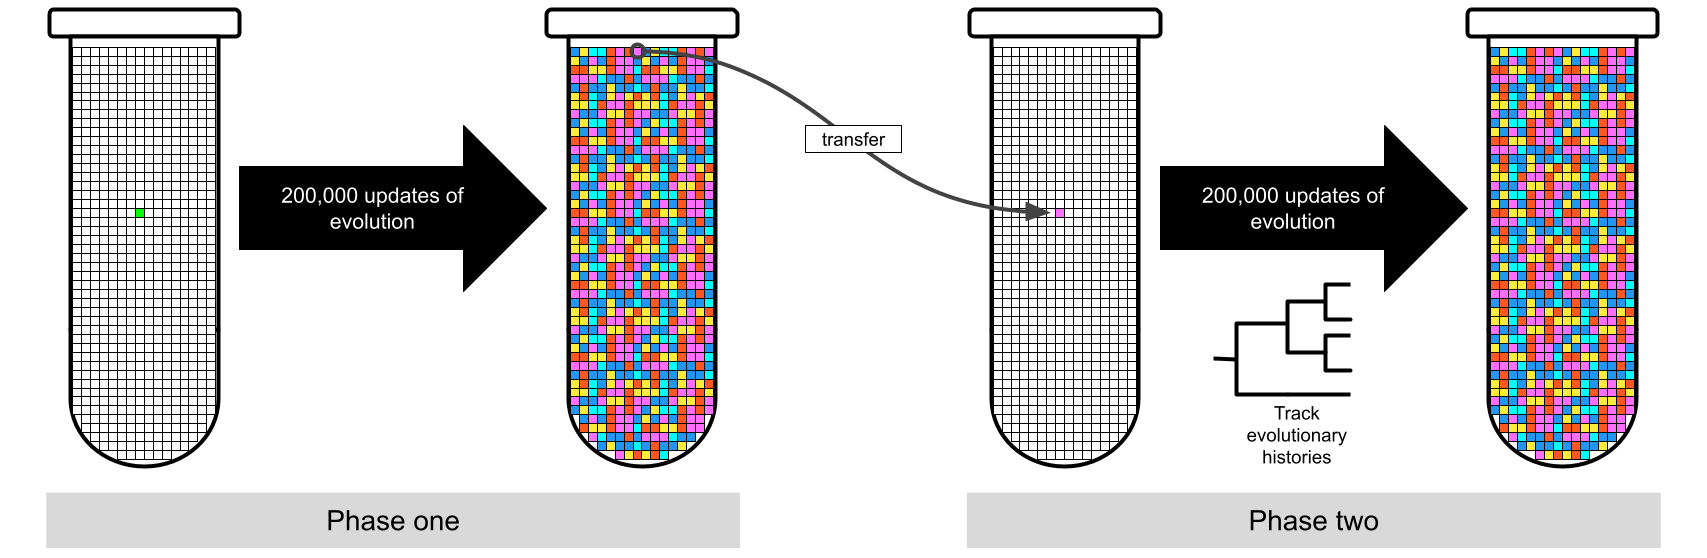
\includegraphics{media/experimental-design-overview.png}
\caption{Experimental design overview}
\end{figure}

\begin{figure}
\centering
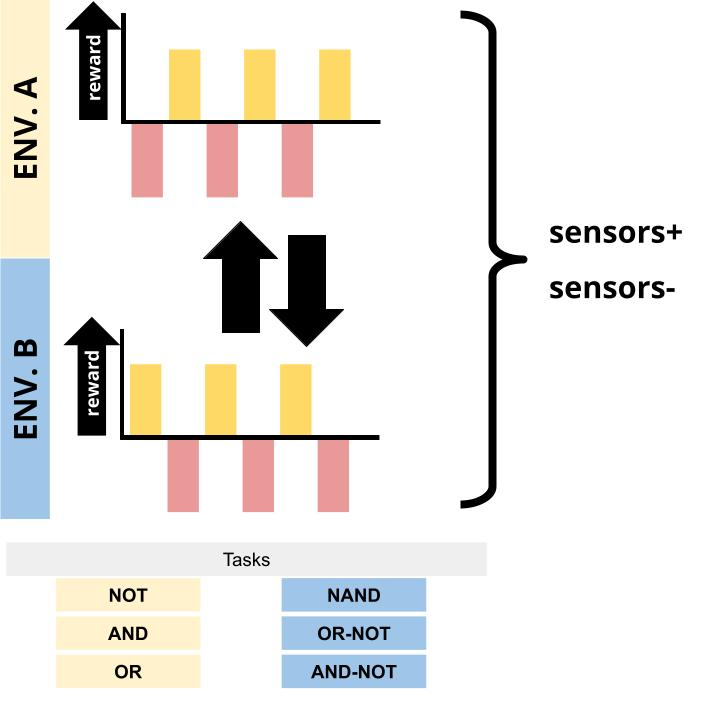
\includegraphics{media/fluctuating-environment.jpg}
\caption{Fluctuating environment}
\end{figure}

\begin{figure}
\centering
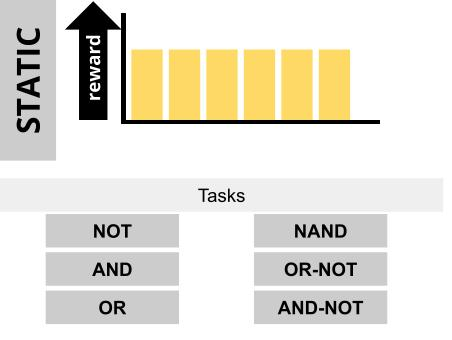
\includegraphics{media/static-environment.jpg}
\caption{Static environment}
\end{figure}

\hypertarget{validation-experiment}{%
\chapter{Validation experiment}\label{validation-experiment}}

In this experiment, we validate that
(1) we observe the evolution of phenotypic plasticity in a changing environment when digital organisms have access to sensory instructions (capable of differentiating environmental states)
and (2) that adaptive phenotypic plasticity does not evolve when populations lack access to sensory instructions.

\hypertarget{overview}{%
\section{Overview}\label{overview}}

\begin{Shaded}
\begin{Highlighting}[]
\NormalTok{total_updates <-}\StringTok{ }\DecValTok{200000}
\NormalTok{replicates <-}\StringTok{ }\DecValTok{100}

\NormalTok{all_traits <-}\StringTok{ }\KeywordTok{c}\NormalTok{(}\StringTok{"not"}\NormalTok{,}\StringTok{"nand"}\NormalTok{,}\StringTok{"and"}\NormalTok{,}\StringTok{"ornot"}\NormalTok{,}\StringTok{"or"}\NormalTok{,}\StringTok{"andnot"}\NormalTok{)}
\NormalTok{traits_set_a <-}\StringTok{ }\KeywordTok{c}\NormalTok{(}\StringTok{"not"}\NormalTok{, }\StringTok{"and"}\NormalTok{, }\StringTok{"or"}\NormalTok{)}
\NormalTok{traits_set_b <-}\StringTok{ }\KeywordTok{c}\NormalTok{(}\StringTok{"nand"}\NormalTok{, }\StringTok{"ornot"}\NormalTok{, }\StringTok{"andnot"}\NormalTok{)}

\CommentTok{# Relative location of data.}
\NormalTok{working_directory <-}\StringTok{ "experiments/2021-01-07-validation/analysis/"} \CommentTok{# << For bookdown}
\CommentTok{# working_directory <- "./"                                              # << For local analysis}
\end{Highlighting}
\end{Shaded}

We evolved populations of digital organisms under four conditions:

\begin{enumerate}
\def\labelenumi{\arabic{enumi}.}
\tightlist
\item
  A fluctuating environment with access to sensory instructions
\item
  A fluctuating environment without access to sensory instructions (i.e., sensory instructions are no-operations)
\item
  A constant environment with access to sensory instructions
\item
  A constant environment without access to sensory instructions
\end{enumerate}

In fluctuating environments, we alternate between rewarding and punishing different sets of computational tasks.
In one environment, we reward tasks not, and, or and punish tasks nand, ornot, andnot.
In the alternative environment, we reward tasks nand, ornot, andnot and punish tasks not, and, or.
In constant environments, we reward all tasks (not, nand, and, ornot, or, andnot).

For each replicate of each condition, we extract the dominant (i.e., most numerous) genotype at the end of the run to analyze further.
We expect to observe the evolution of adaptive phenotypic plasticity in only the first experimental condition.
In conditions without sensors, plasticity in any form should be unable to evolve.

\hypertarget{analysis-dependencies}{%
\section{Analysis dependencies}\label{analysis-dependencies}}

Load all required R libraries.

\begin{Shaded}
\begin{Highlighting}[]
\KeywordTok{library}\NormalTok{(ggplot2)}
\KeywordTok{library}\NormalTok{(tidyverse)}
\KeywordTok{library}\NormalTok{(cowplot)}
\KeywordTok{source}\NormalTok{(}\StringTok{"https://gist.githubusercontent.com/benmarwick/2a1bb0133ff568cbe28d/raw/fb53bd97121f7f9ce947837ef1a4c65a73bffb3f/geom_flat_violin.R"}\NormalTok{)}
\end{Highlighting}
\end{Shaded}

These analyses were conducted/knitted with the following computing environment:

\begin{Shaded}
\begin{Highlighting}[]
\KeywordTok{print}\NormalTok{(version)}
\end{Highlighting}
\end{Shaded}

\begin{verbatim}
##                _                           
## platform       x86_64-pc-linux-gnu         
## arch           x86_64                      
## os             linux-gnu                   
## system         x86_64, linux-gnu           
## status                                     
## major          4                           
## minor          0.4                         
## year           2021                        
## month          02                          
## day            15                          
## svn rev        80002                       
## language       R                           
## version.string R version 4.0.4 (2021-02-15)
## nickname       Lost Library Book
\end{verbatim}

\hypertarget{setup}{%
\section{Setup}\label{setup}}

\begin{Shaded}
\begin{Highlighting}[]
\NormalTok{data_loc <-}\StringTok{ }\KeywordTok{paste0}\NormalTok{(working_directory, }\StringTok{"data/aggregate.csv"}\NormalTok{)}
\NormalTok{data <-}\StringTok{ }\KeywordTok{read.csv}\NormalTok{(data_loc, }\DataTypeTok{na.strings=}\StringTok{"NONE"}\NormalTok{)}

\NormalTok{data}\OperatorTok{$}\NormalTok{DISABLE_REACTION_SENSORS <-}\StringTok{ }\KeywordTok{as.factor}\NormalTok{(data}\OperatorTok{$}\NormalTok{DISABLE_REACTION_SENSORS)}
\NormalTok{data}\OperatorTok{$}\NormalTok{chg_env <-}\StringTok{ }\KeywordTok{as.factor}\NormalTok{(data}\OperatorTok{$}\NormalTok{chg_env)}
\NormalTok{data}\OperatorTok{$}\NormalTok{dom_plastic_odd_even <-}\StringTok{ }\KeywordTok{as.factor}\NormalTok{(data}\OperatorTok{$}\NormalTok{dom_plastic_odd_even)}
\NormalTok{data}\OperatorTok{$}\NormalTok{sensors <-}\StringTok{ }\NormalTok{data}\OperatorTok{$}\NormalTok{DISABLE_REACTION_SENSORS }\OperatorTok{==}\StringTok{ "0"}
\NormalTok{data}\OperatorTok{$}\NormalTok{is_plastic <-}\StringTok{ }\NormalTok{data}\OperatorTok{$}\NormalTok{dom_plastic_odd_even }\OperatorTok{==}\StringTok{ "True"}

\NormalTok{env_label_fun <-}\StringTok{ }\ControlFlowTok{function}\NormalTok{(chg_env) \{}
  \ControlFlowTok{if}\NormalTok{ (chg_env) \{}
    \KeywordTok{return}\NormalTok{(}\StringTok{"Fluctuating"}\NormalTok{)}
\NormalTok{  \} }\ControlFlowTok{else}\NormalTok{ \{}
    \KeywordTok{return}\NormalTok{(}\StringTok{"Constant"}\NormalTok{)}
\NormalTok{  \}}
\NormalTok{\}}

\NormalTok{sensors_label_fun <-}\StringTok{ }\ControlFlowTok{function}\NormalTok{(has_sensors) \{}
  \ControlFlowTok{if}\NormalTok{ (has_sensors) \{}
    \KeywordTok{return}\NormalTok{(}\StringTok{"Sensors"}\NormalTok{)}
\NormalTok{  \} }\ControlFlowTok{else}\NormalTok{ \{}
    \KeywordTok{return}\NormalTok{(}\StringTok{"No sensors"}\NormalTok{)}
\NormalTok{  \}}
\NormalTok{\}}

\CommentTok{# Count observed plasticity for each condition (I'm sure there's a 'tidier' way to do this..)}
\NormalTok{observed_plasticity <-}\StringTok{ }\KeywordTok{data.frame}\NormalTok{(}
  \DataTypeTok{environment=}\KeywordTok{character}\NormalTok{(),}
  \DataTypeTok{sensors=}\KeywordTok{character}\NormalTok{(),}
  \DataTypeTok{plastic=}\KeywordTok{integer}\NormalTok{(),}
  \DataTypeTok{nonplastic=}\KeywordTok{integer}\NormalTok{(),}
  \DataTypeTok{plastic_adaptive=}\KeywordTok{integer}\NormalTok{(),}
  \DataTypeTok{plastic_optimal=}\KeywordTok{integer}\NormalTok{(),}
  \DataTypeTok{plastic_nonadaptive=}\KeywordTok{integer}\NormalTok{()}
\NormalTok{)}
\ControlFlowTok{for}\NormalTok{ (env_chg }\ControlFlowTok{in} \KeywordTok{levels}\NormalTok{(data}\OperatorTok{$}\NormalTok{chg_env)) \{}
  \ControlFlowTok{for}\NormalTok{ (disabled_sensors }\ControlFlowTok{in} \KeywordTok{levels}\NormalTok{(data}\OperatorTok{$}\NormalTok{DISABLE_REACTION_SENSORS)) \{}
\NormalTok{    cond_data <-}\StringTok{ }\KeywordTok{filter}\NormalTok{(data, chg_env }\OperatorTok{==}\StringTok{ }\NormalTok{env_chg }\OperatorTok{&}\StringTok{ }\NormalTok{data}\OperatorTok{$}\NormalTok{DISABLE_REACTION_SENSORS }\OperatorTok{==}\StringTok{ }\NormalTok{disabled_sensors)}
\NormalTok{    environment_label <-}\StringTok{ }\KeywordTok{env_label_fun}\NormalTok{(env_chg)}
\NormalTok{    sensors_label <-}\StringTok{ }\KeywordTok{sensors_label_fun}\NormalTok{(disabled_sensors }\OperatorTok{==}\StringTok{ "0"}\NormalTok{)}

\NormalTok{    observed_plasticity <-}\StringTok{ }\NormalTok{observed_plasticity }\OperatorTok\StringTok{ }\KeywordTok{add_row}\NormalTok{(}
      \DataTypeTok{environment=}\NormalTok{environment_label,}
      \DataTypeTok{sensors=}\NormalTok{sensors_label,}
      \DataTypeTok{plastic=}\KeywordTok{nrow}\NormalTok{(}\KeywordTok{filter}\NormalTok{(cond_data, is_plastic}\OperatorTok{==}\OtherTok{TRUE}\NormalTok{)),}
      \DataTypeTok{nonplastic=}\KeywordTok{nrow}\NormalTok{(}\KeywordTok{filter}\NormalTok{(cond_data, is_plastic}\OperatorTok{==}\OtherTok{FALSE}\NormalTok{)),}
      \DataTypeTok{plastic_adaptive=}\KeywordTok{nrow}\NormalTok{(}\KeywordTok{filter}\NormalTok{(cond_data, dom_adaptive_plasticity}\OperatorTok{==}\StringTok{"True"}\NormalTok{)),}
      \DataTypeTok{plastic_optimal=}\KeywordTok{nrow}\NormalTok{(}\KeywordTok{filter}\NormalTok{(cond_data, dom_optimal_plastic}\OperatorTok{==}\StringTok{"True"}\NormalTok{)),}
      \DataTypeTok{plastic_nonadaptive=}\KeywordTok{nrow}\NormalTok{(}\KeywordTok{filter}\NormalTok{(cond_data, is_plastic}\OperatorTok{==}\OtherTok{TRUE} \OperatorTok{&}\StringTok{ }\NormalTok{dom_adaptive_plasticity}\OperatorTok{==}\StringTok{"False"}\NormalTok{))}
\NormalTok{    )}
\NormalTok{  \}}
\NormalTok{\}}

\NormalTok{observed_plasticity <-}\StringTok{ }\KeywordTok{pivot_longer}\NormalTok{(}
\NormalTok{  observed_plasticity,}
  \DataTypeTok{cols=}\KeywordTok{c}\NormalTok{(}\StringTok{"plastic"}\NormalTok{, }\StringTok{"plastic_adaptive"}\NormalTok{, }\StringTok{"plastic_optimal"}\NormalTok{, }\StringTok{"plastic_nonadaptive"}\NormalTok{, }\StringTok{"nonplastic"}\NormalTok{),}
  \DataTypeTok{names_to=}\StringTok{"phenotype"}\NormalTok{,}
  \DataTypeTok{values_to=}\StringTok{"phenotype_cnt"}
\NormalTok{)}

\CommentTok{####### misc #######}
\CommentTok{# Configure our default graphing theme}
\KeywordTok{theme_set}\NormalTok{(}\KeywordTok{theme_cowplot}\NormalTok{())}
\end{Highlighting}
\end{Shaded}

\hypertarget{evolution-of-phenotypic-plasticity}{%
\section{Evolution of phenotypic plasticity}\label{evolution-of-phenotypic-plasticity}}

For each experimental condition, do we observe the evolution of phenotypic plasticity? To test for phenotypic plasticity, we culture digital organisms in both environments from the fluctuating condition (including organisms evolved in a constant environment).
Any plasticity that we observe from digital organisms evolved under constant conditions is cryptic variation (as these organisms were never exposed to these culturing environments).

\begin{Shaded}
\begin{Highlighting}[]
\KeywordTok{ggplot}\NormalTok{(}\KeywordTok{filter}\NormalTok{(observed_plasticity, phenotype }\OperatorTok\StringTok{ }\KeywordTok{c}\NormalTok{(}\StringTok{"plastic"}\NormalTok{, }\StringTok{"nonplastic"}\NormalTok{)), }\KeywordTok{aes}\NormalTok{(}\DataTypeTok{x=}\NormalTok{phenotype, }\DataTypeTok{y=}\NormalTok{phenotype_cnt, }\DataTypeTok{fill=}\NormalTok{phenotype)) }\OperatorTok{+}
\StringTok{  }\KeywordTok{geom_bar}\NormalTok{(}
    \DataTypeTok{stat=}\StringTok{"identity"}\NormalTok{,}
    \DataTypeTok{position=}\KeywordTok{position_dodge}\NormalTok{(}\FloatTok{0.9}\NormalTok{)}
\NormalTok{  ) }\OperatorTok{+}
\StringTok{  }\KeywordTok{geom_text}\NormalTok{(}
    \DataTypeTok{stat=}\StringTok{"identity"}\NormalTok{,}
    \DataTypeTok{mapping=}\KeywordTok{aes}\NormalTok{(}\DataTypeTok{label=}\NormalTok{phenotype_cnt),}
    \DataTypeTok{vjust=}\FloatTok{0.05}
\NormalTok{  ) }\OperatorTok{+}
\StringTok{  }\KeywordTok{scale_fill_brewer}\NormalTok{(}\DataTypeTok{palette=}\StringTok{"Accent"}\NormalTok{) }\OperatorTok{+}
\StringTok{  }\KeywordTok{scale_x_discrete}\NormalTok{(}
    \DataTypeTok{name=}\StringTok{"Phenotype"}\NormalTok{,}
    \DataTypeTok{limits=}\KeywordTok{c}\NormalTok{(}\StringTok{"plastic"}\NormalTok{, }\StringTok{"nonplastic"}\NormalTok{),}
    \DataTypeTok{labels=}\KeywordTok{c}\NormalTok{(}\StringTok{"Plastic"}\NormalTok{, }\StringTok{"Non-plastic"}\NormalTok{)}
\NormalTok{  ) }\OperatorTok{+}
\StringTok{  }\KeywordTok{facet_grid}\NormalTok{(sensors}\OperatorTok{~}\NormalTok{environment) }\OperatorTok{+}
\StringTok{  }\KeywordTok{theme}\NormalTok{(}
    \DataTypeTok{legend.position=}\StringTok{"none"}
\NormalTok{  )}
\end{Highlighting}
\end{Shaded}

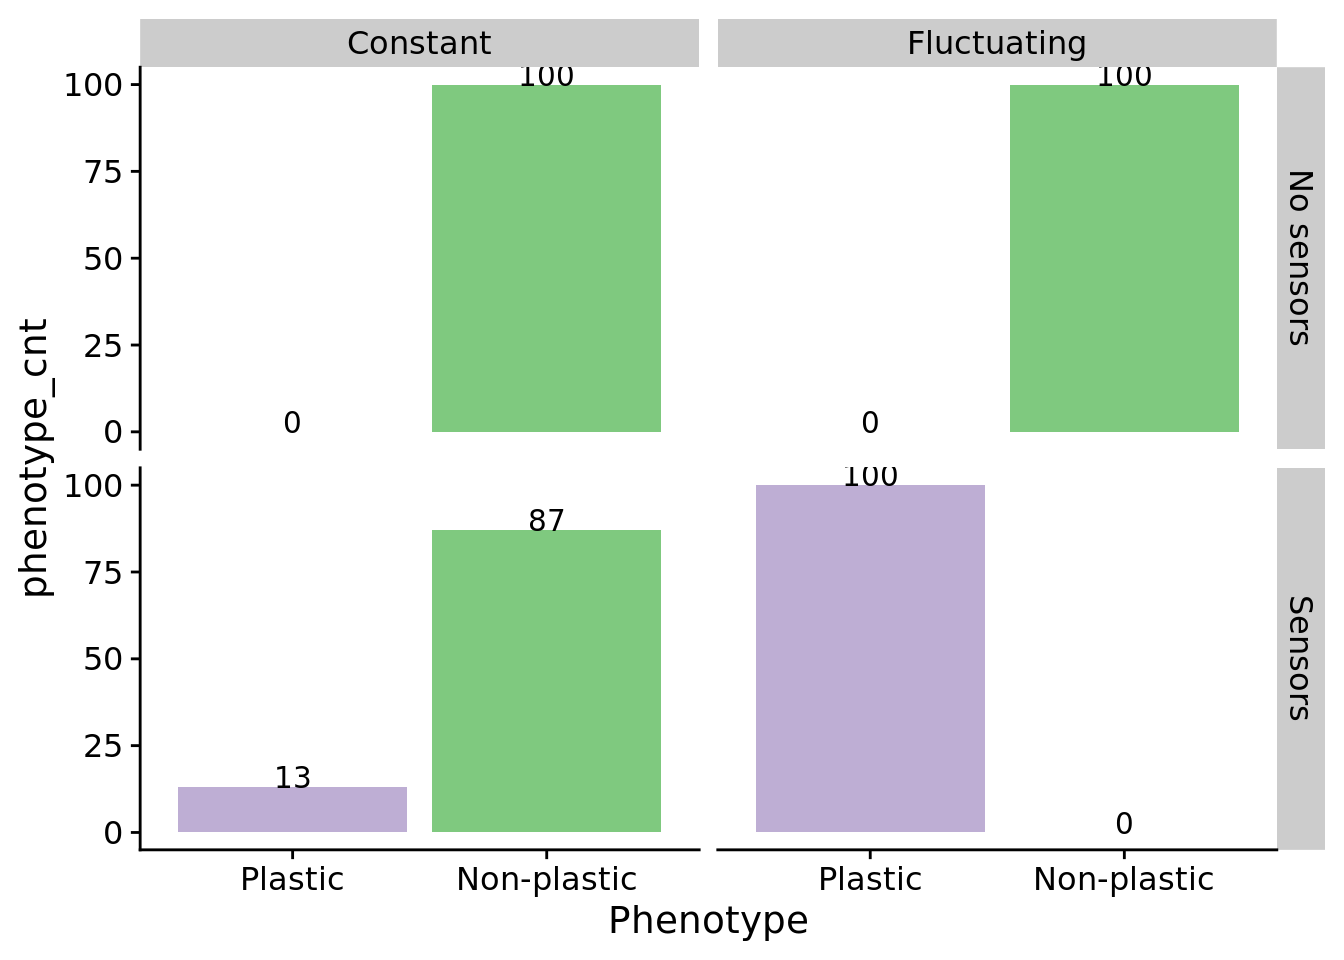
\includegraphics{supplemental-material_files/figure-latex/unnamed-chunk-5-1.pdf}

Indeed, we do not observe the evolution of phenotypic plasticity in any replicates in which digital organisms do not have access to sensory instructions.
We do observe the evolution of plasticity (not necessarily adaptive plasticity) in both constant and fluctuating environments where sensors are enabled.

To what extent is the observed phenotypic plasticity adaptive?

\begin{Shaded}
\begin{Highlighting}[]
\KeywordTok{ggplot}\NormalTok{(}\KeywordTok{filter}\NormalTok{(observed_plasticity, environment}\OperatorTok{==}\StringTok{"Fluctuating"} \OperatorTok{&}\StringTok{ }\NormalTok{sensors }\OperatorTok{==}\StringTok{ "Sensors"} \OperatorTok{&}\StringTok{ }\NormalTok{phenotype }\OperatorTok\StringTok{ }\KeywordTok{c}\NormalTok{(}\StringTok{"plastic"}\NormalTok{, }\StringTok{"plastic_adaptive"}\NormalTok{, }\StringTok{"plastic_optimal"}\NormalTok{, }\StringTok{"plastic_nonadaptive"}\NormalTok{)), }\KeywordTok{aes}\NormalTok{(}\DataTypeTok{x=}\NormalTok{phenotype, }\DataTypeTok{y=}\NormalTok{phenotype_cnt, }\DataTypeTok{fill=}\NormalTok{phenotype)) }\OperatorTok{+}
\StringTok{  }\KeywordTok{geom_bar}\NormalTok{(}
    \DataTypeTok{stat=}\StringTok{"identity"}\NormalTok{,}
    \DataTypeTok{position=}\KeywordTok{position_dodge}\NormalTok{(}\FloatTok{0.9}\NormalTok{)}
\NormalTok{  ) }\OperatorTok{+}
\StringTok{  }\KeywordTok{geom_text}\NormalTok{(}
    \DataTypeTok{stat=}\StringTok{"identity"}\NormalTok{,}
    \DataTypeTok{mapping=}\KeywordTok{aes}\NormalTok{(}\DataTypeTok{label=}\NormalTok{phenotype_cnt),}
    \DataTypeTok{vjust=}\FloatTok{0.05}
\NormalTok{  ) }\OperatorTok{+}
\StringTok{  }\KeywordTok{scale_fill_brewer}\NormalTok{(}\DataTypeTok{palette=}\StringTok{"Accent"}\NormalTok{) }\OperatorTok{+}
\StringTok{  }\KeywordTok{scale_x_discrete}\NormalTok{(}
    \DataTypeTok{name=}\StringTok{"Phenotype"}\NormalTok{,}
    \DataTypeTok{limits=}\KeywordTok{c}\NormalTok{(}\StringTok{"plastic"}\NormalTok{,  }\StringTok{"plastic_adaptive"}\NormalTok{, }\StringTok{"plastic_optimal"}\NormalTok{, }\StringTok{"plastic_nonadaptive"}\NormalTok{),}
    \DataTypeTok{labels=}\KeywordTok{c}\NormalTok{(}\StringTok{"Total plastic"}\NormalTok{, }\StringTok{"Adaptive plasticity"}\NormalTok{, }\StringTok{"Optimal plasticity"}\NormalTok{, }\StringTok{"Non-adaptive plasticity"}\NormalTok{)}
\NormalTok{  ) }\OperatorTok{+}
\StringTok{  }\KeywordTok{facet_grid}\NormalTok{(sensors}\OperatorTok{~}\NormalTok{environment) }\OperatorTok{+}
\StringTok{  }\KeywordTok{theme}\NormalTok{(}
    \DataTypeTok{legend.position=}\StringTok{"none"}
\NormalTok{  )}
\end{Highlighting}
\end{Shaded}

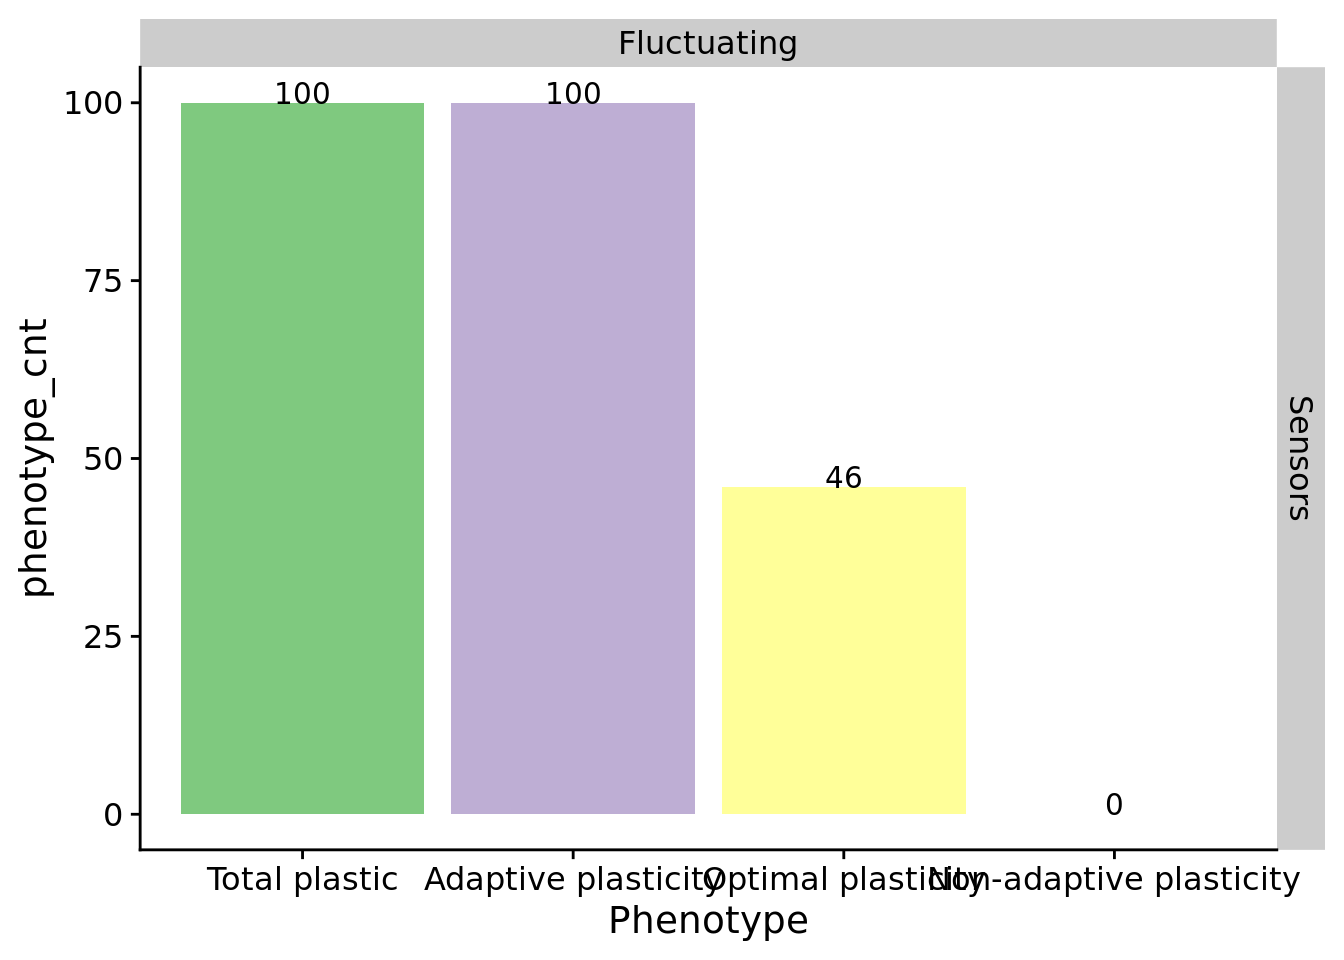
\includegraphics{supplemental-material_files/figure-latex/unnamed-chunk-6-1.pdf}

\hypertarget{evolutionary-change}{%
\chapter{Evolutionary change}\label{evolutionary-change}}

The effect of adaptive phenotypic plasticity on evolutionary change.

\hypertarget{overview-1}{%
\section{Overview}\label{overview-1}}

\begin{Shaded}
\begin{Highlighting}[]
\NormalTok{total_updates <-}\StringTok{ }\DecValTok{200000}
\NormalTok{replicates <-}\StringTok{ }\DecValTok{100}

\NormalTok{all_traits <-}\StringTok{ }\KeywordTok{c}\NormalTok{(}\StringTok{"not"}\NormalTok{,}\StringTok{"nand"}\NormalTok{,}\StringTok{"and"}\NormalTok{,}\StringTok{"ornot"}\NormalTok{,}\StringTok{"or"}\NormalTok{,}\StringTok{"andnot"}\NormalTok{)}
\NormalTok{traits_set_a <-}\StringTok{ }\KeywordTok{c}\NormalTok{(}\StringTok{"not"}\NormalTok{, }\StringTok{"and"}\NormalTok{, }\StringTok{"or"}\NormalTok{)}
\NormalTok{traits_set_b <-}\StringTok{ }\KeywordTok{c}\NormalTok{(}\StringTok{"nand"}\NormalTok{, }\StringTok{"ornot"}\NormalTok{, }\StringTok{"andnot"}\NormalTok{)}

\CommentTok{# Relative location of data.}
\NormalTok{working_directory <-}\StringTok{ "experiments/2021-02-08-evo-dynamics/analysis/"} \CommentTok{# << For bookdown}
\CommentTok{# working_directory <- "./"                                              # << For local analysis}
\end{Highlighting}
\end{Shaded}

\hypertarget{analysis-dependencies-1}{%
\section{Analysis dependencies}\label{analysis-dependencies-1}}

Load all required R libraries.

\begin{Shaded}
\begin{Highlighting}[]
\KeywordTok{library}\NormalTok{(ggplot2)}
\KeywordTok{library}\NormalTok{(tidyverse)}
\KeywordTok{library}\NormalTok{(cowplot)}
\KeywordTok{library}\NormalTok{(RColorBrewer)}
\KeywordTok{library}\NormalTok{(Hmisc)}
\KeywordTok{library}\NormalTok{(boot)}
\KeywordTok{source}\NormalTok{(}\StringTok{"https://gist.githubusercontent.com/benmarwick/2a1bb0133ff568cbe28d/raw/fb53bd97121f7f9ce947837ef1a4c65a73bffb3f/geom_flat_violin.R"}\NormalTok{)}
\end{Highlighting}
\end{Shaded}

These analyses were conducted/knitted with the following computing environment:

\begin{Shaded}
\begin{Highlighting}[]
\KeywordTok{print}\NormalTok{(version)}
\end{Highlighting}
\end{Shaded}

\begin{verbatim}
##                _                           
## platform       x86_64-pc-linux-gnu         
## arch           x86_64                      
## os             linux-gnu                   
## system         x86_64, linux-gnu           
## status                                     
## major          4                           
## minor          0.4                         
## year           2021                        
## month          02                          
## day            15                          
## svn rev        80002                       
## language       R                           
## version.string R version 4.0.4 (2021-02-15)
## nickname       Lost Library Book
\end{verbatim}

\hypertarget{setup-1}{%
\section{Setup}\label{setup-1}}

\begin{Shaded}
\begin{Highlighting}[]
\NormalTok{summary_data_loc <-}\StringTok{ }\KeywordTok{paste0}\NormalTok{(working_directory, }\StringTok{"data/aggregate.csv"}\NormalTok{)}
\NormalTok{summary_data <-}\StringTok{ }\KeywordTok{read.csv}\NormalTok{(summary_data_loc, }\DataTypeTok{na.strings=}\StringTok{"NONE"}\NormalTok{)}

\NormalTok{summary_data}\OperatorTok{$}\NormalTok{DISABLE_REACTION_SENSORS <-}\StringTok{ }\KeywordTok{as.factor}\NormalTok{(summary_data}\OperatorTok{$}\NormalTok{DISABLE_REACTION_SENSORS)}
\NormalTok{summary_data}\OperatorTok{$}\NormalTok{chg_env <-}\StringTok{ }\NormalTok{summary_data}\OperatorTok{$}\NormalTok{chg_env }\OperatorTok{==}\StringTok{ "True"}
\NormalTok{summary_data}\OperatorTok{$}\NormalTok{dominant_plastic_odd_even <-}\StringTok{ }\KeywordTok{as.factor}\NormalTok{(summary_data}\OperatorTok{$}\NormalTok{dominant_plastic_odd_even)}
\NormalTok{summary_data}\OperatorTok{$}\NormalTok{sensors <-}\StringTok{ }\NormalTok{summary_data}\OperatorTok{$}\NormalTok{DISABLE_REACTION_SENSORS }\OperatorTok{==}\StringTok{ "0"}
\NormalTok{summary_data}\OperatorTok{$}\NormalTok{is_plastic <-}\StringTok{ }\NormalTok{summary_data}\OperatorTok{$}\NormalTok{dominant_plastic_odd_even }\OperatorTok{==}\StringTok{ "True"}

\NormalTok{env_label_fun <-}\StringTok{ }\ControlFlowTok{function}\NormalTok{(chg_env) \{}
  \ControlFlowTok{if}\NormalTok{ (chg_env) \{}
    \KeywordTok{return}\NormalTok{(}\StringTok{"Fluctuating"}\NormalTok{)}
\NormalTok{  \} }\ControlFlowTok{else}\NormalTok{ \{}
    \KeywordTok{return}\NormalTok{(}\StringTok{"Constant"}\NormalTok{)}
\NormalTok{  \}}
\NormalTok{\}}

\NormalTok{sensors_label_fun <-}\StringTok{ }\ControlFlowTok{function}\NormalTok{(has_sensors) \{}
  \ControlFlowTok{if}\NormalTok{ (has_sensors) \{}
    \KeywordTok{return}\NormalTok{(}\StringTok{"Sensors"}\NormalTok{)}
\NormalTok{  \} }\ControlFlowTok{else}\NormalTok{ \{}
    \KeywordTok{return}\NormalTok{(}\StringTok{"No sensors"}\NormalTok{)}
\NormalTok{  \}}
\NormalTok{\}}

\CommentTok{# note that this labeler makes assumptions about how we set up our experiment}
\NormalTok{condition_label_fun <-}\StringTok{ }\ControlFlowTok{function}\NormalTok{(has_sensors, env_chg) \{}
  \ControlFlowTok{if}\NormalTok{ (has_sensors }\OperatorTok{&&}\StringTok{ }\NormalTok{env_chg) \{}
    \KeywordTok{return}\NormalTok{(}\StringTok{"PLASTIC"}\NormalTok{)}
\NormalTok{  \} }\ControlFlowTok{else} \ControlFlowTok{if}\NormalTok{ (env_chg) \{}
    \KeywordTok{return}\NormalTok{(}\StringTok{"NON-PLASTIC"}\NormalTok{)}
\NormalTok{  \} }\ControlFlowTok{else}\NormalTok{ \{}
    \KeywordTok{return}\NormalTok{(}\StringTok{"STATIC"}\NormalTok{)}
\NormalTok{  \}}
\NormalTok{\}}

\NormalTok{summary_data}\OperatorTok{$}\NormalTok{env_label <-}\StringTok{ }\KeywordTok{mapply}\NormalTok{(}
\NormalTok{  env_label_fun,}
\NormalTok{  summary_data}\OperatorTok{$}\NormalTok{chg_env}
\NormalTok{)}
\NormalTok{summary_data}\OperatorTok{$}\NormalTok{sensors_label <-}\StringTok{ }\KeywordTok{mapply}\NormalTok{(}
\NormalTok{  sensors_label_fun,}
\NormalTok{  summary_data}\OperatorTok{$}\NormalTok{sensors}
\NormalTok{)}
\NormalTok{summary_data}\OperatorTok{$}\NormalTok{condition <-}\StringTok{ }\KeywordTok{mapply}\NormalTok{(}
\NormalTok{  condition_label_fun,}
\NormalTok{  summary_data}\OperatorTok{$}\NormalTok{sensors,}
\NormalTok{  summary_data}\OperatorTok{$}\NormalTok{chg_env}
\NormalTok{)}

\NormalTok{condition_order =}\StringTok{ }\KeywordTok{c}\NormalTok{(}
  \StringTok{"STATIC"}\NormalTok{,}
  \StringTok{"NON-PLASTIC"}\NormalTok{,}
  \StringTok{"PLASTIC"}
\NormalTok{)}

\CommentTok{####### misc #######}
\CommentTok{# Configure our default graphing theme}
\KeywordTok{theme_set}\NormalTok{(}\KeywordTok{theme_cowplot}\NormalTok{())}
\KeywordTok{dir.create}\NormalTok{(}\KeywordTok{paste0}\NormalTok{(working_directory, }\StringTok{"plots"}\NormalTok{), }\DataTypeTok{showWarnings=}\OtherTok{FALSE}\NormalTok{)}
\end{Highlighting}
\end{Shaded}

\hypertarget{evolution-of-phenotypic-plasticity-1}{%
\section{Evolution of phenotypic plasticity}\label{evolution-of-phenotypic-plasticity-1}}

For sensor-enabled populations in fluctuating environments, we only transfered populations containing an optimally plastic genotype to phase-two.

\begin{Shaded}
\begin{Highlighting}[]
\NormalTok{summary_data_grouped =}\StringTok{ }\NormalTok{dplyr}\OperatorTok{::}\KeywordTok{group_by}\NormalTok{(summary_data, condition)}
\NormalTok{summary_data_group_counts =}\StringTok{ }\NormalTok{dplyr}\OperatorTok{::}\KeywordTok{summarize}\NormalTok{(summary_data_grouped, }\DataTypeTok{n=}\NormalTok{dplyr}\OperatorTok{::}\KeywordTok{n}\NormalTok{())}

\KeywordTok{ggplot}\NormalTok{(summary_data_group_counts, }\KeywordTok{aes}\NormalTok{(}\DataTypeTok{x=}\NormalTok{condition, }\DataTypeTok{y=}\NormalTok{n, }\DataTypeTok{fill=}\NormalTok{condition)) }\OperatorTok{+}
\StringTok{  }\KeywordTok{geom_col}\NormalTok{(}\DataTypeTok{position=}\KeywordTok{position_dodge}\NormalTok{(}\FloatTok{0.9}\NormalTok{)) }\OperatorTok{+}
\StringTok{  }\KeywordTok{geom_text}\NormalTok{(}\KeywordTok{aes}\NormalTok{(}\DataTypeTok{label=}\NormalTok{n, }\DataTypeTok{y=}\NormalTok{n}\OperatorTok{+}\DecValTok{2}\NormalTok{)) }\OperatorTok{+}
\StringTok{  }\KeywordTok{scale_x_discrete}\NormalTok{(}
    \DataTypeTok{name=}\StringTok{"Condition"}\NormalTok{,}
    \DataTypeTok{limits=}\NormalTok{condition_order}
\NormalTok{  ) }\OperatorTok{+}
\StringTok{  }\KeywordTok{ylab}\NormalTok{(}\StringTok{"Number of replicates in phase two"}\NormalTok{) }\OperatorTok{+}
\StringTok{  }\KeywordTok{theme}\NormalTok{(}
    \DataTypeTok{legend.position=}\StringTok{"none"}
\NormalTok{  )}
\end{Highlighting}
\end{Shaded}

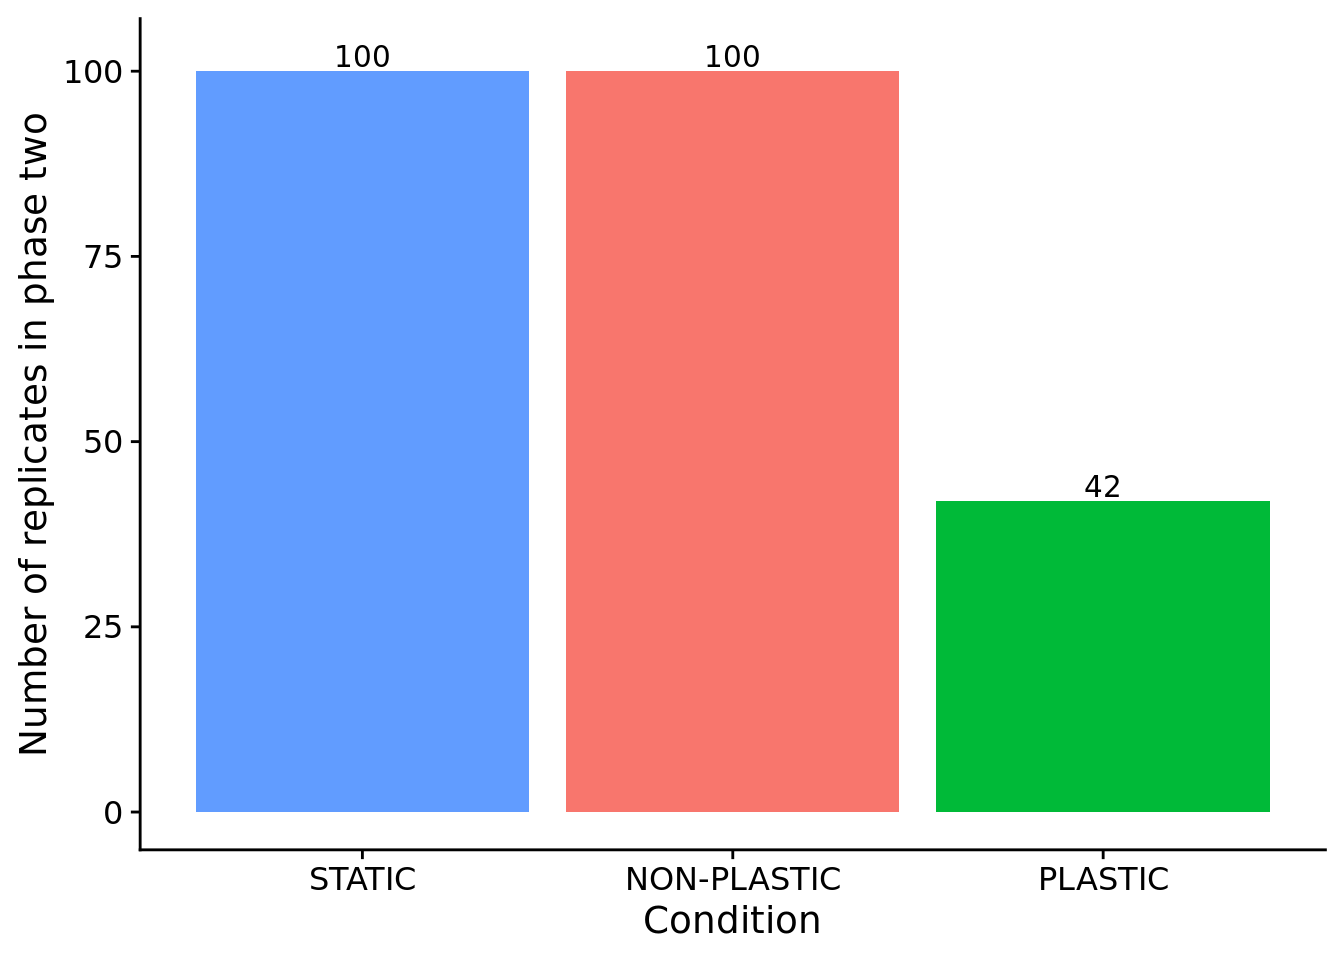
\includegraphics{supplemental-material_files/figure-latex/unnamed-chunk-11-1.pdf}

We can confirm our expectation that the dominant genotypes in non-plastic conditions are not phenotypically plastic.

\begin{Shaded}
\begin{Highlighting}[]
\NormalTok{summary_data_grouped =}\StringTok{ }\NormalTok{dplyr}\OperatorTok{::}\KeywordTok{group_by}\NormalTok{(summary_data, condition, is_plastic)}
\NormalTok{summary_data_group_counts =}\StringTok{ }\NormalTok{dplyr}\OperatorTok{::}\KeywordTok{summarize}\NormalTok{(summary_data_grouped, }\DataTypeTok{n=}\NormalTok{dplyr}\OperatorTok{::}\KeywordTok{n}\NormalTok{())}
\KeywordTok{ggplot}\NormalTok{(}\KeywordTok{filter}\NormalTok{(summary_data_group_counts, is_plastic), }\KeywordTok{aes}\NormalTok{(}\DataTypeTok{x=}\NormalTok{condition, }\DataTypeTok{y=}\NormalTok{n, }\DataTypeTok{fill=}\NormalTok{condition)) }\OperatorTok{+}
\StringTok{  }\KeywordTok{geom_col}\NormalTok{(}
    \DataTypeTok{position=}\KeywordTok{position_dodge}\NormalTok{(}\FloatTok{0.9}\NormalTok{)}
\NormalTok{  ) }\OperatorTok{+}
\StringTok{  }\KeywordTok{scale_x_discrete}\NormalTok{(}
    \DataTypeTok{name=}\StringTok{"Condition"}\NormalTok{,}
    \DataTypeTok{limits=}\NormalTok{condition_order}
\NormalTok{  ) }\OperatorTok{+}
\StringTok{  }\KeywordTok{geom_text}\NormalTok{(}\KeywordTok{aes}\NormalTok{(}\DataTypeTok{label=}\NormalTok{n, }\DataTypeTok{y=}\NormalTok{n}\OperatorTok{+}\DecValTok{1}\NormalTok{)) }\OperatorTok{+}
\StringTok{  }\KeywordTok{ylab}\NormalTok{(}\StringTok{"Number of plastic replicates"}\NormalTok{) }\OperatorTok{+}
\StringTok{  }\KeywordTok{ylim}\NormalTok{(}\DecValTok{0}\NormalTok{, }\DecValTok{100}\NormalTok{) }\OperatorTok{+}
\StringTok{  }\KeywordTok{theme}\NormalTok{(}
    \DataTypeTok{legend.position=}\StringTok{"none"}
\NormalTok{  )}
\end{Highlighting}
\end{Shaded}

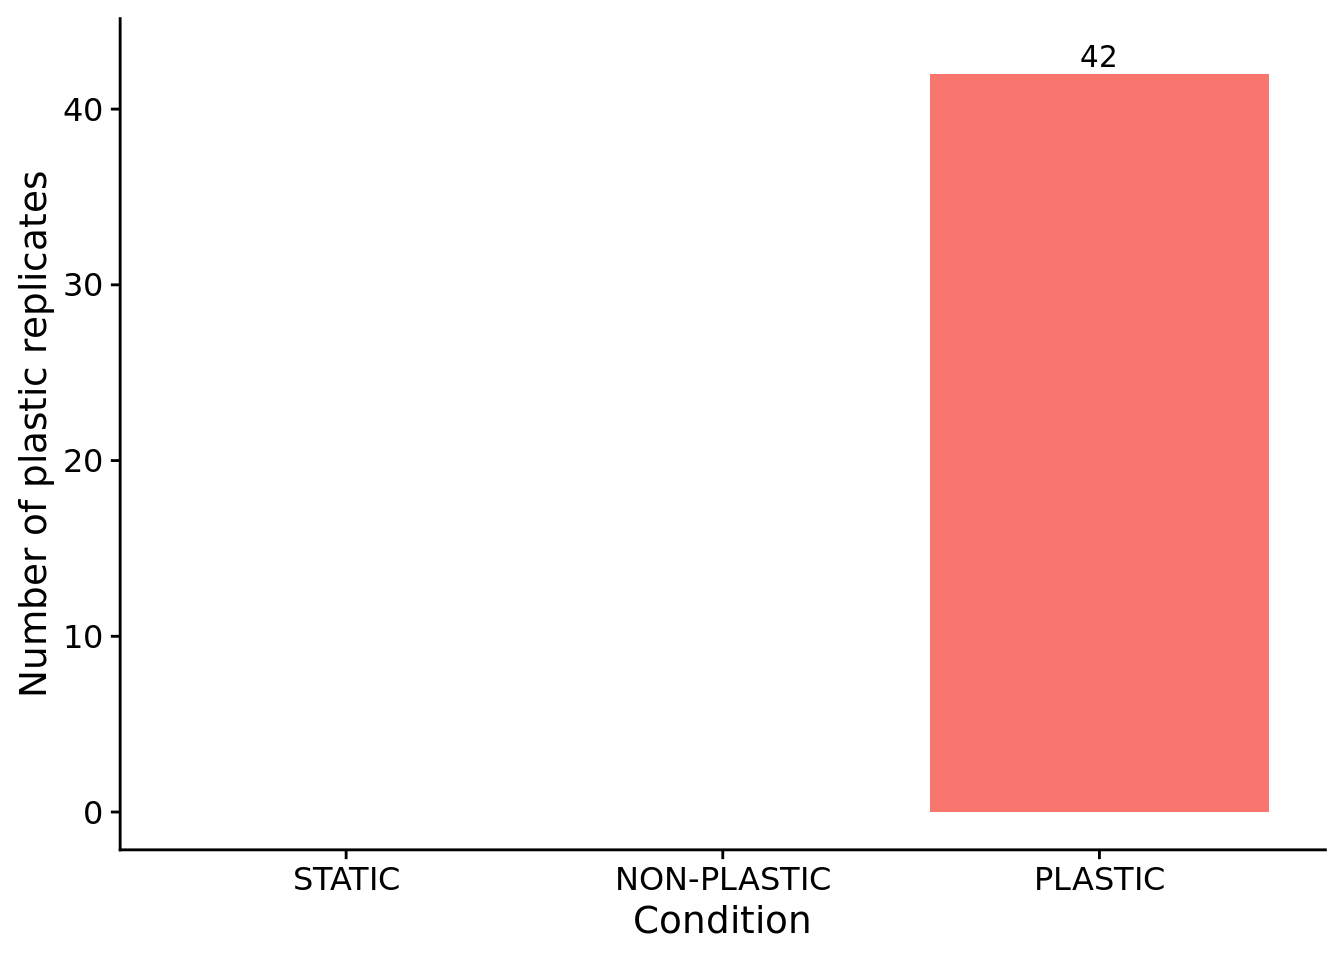
\includegraphics{supplemental-material_files/figure-latex/unnamed-chunk-12-1.pdf}

\hypertarget{average-generation}{%
\section{Average generation}\label{average-generation}}

\begin{Shaded}
\begin{Highlighting}[]
\KeywordTok{ggplot}\NormalTok{(summary_data, }\KeywordTok{aes}\NormalTok{(}\DataTypeTok{x=}\NormalTok{condition, }\DataTypeTok{y=}\NormalTok{time_average_generation, }\DataTypeTok{fill=}\NormalTok{condition)) }\OperatorTok{+}
\StringTok{  }\KeywordTok{geom_flat_violin}\NormalTok{(}
    \DataTypeTok{position =} \KeywordTok{position_nudge}\NormalTok{(}\DataTypeTok{x =} \FloatTok{.2}\NormalTok{, }\DataTypeTok{y =} \DecValTok{0}\NormalTok{),}
    \DataTypeTok{alpha =} \FloatTok{.8}
\NormalTok{  ) }\OperatorTok{+}
\StringTok{  }\KeywordTok{geom_point}\NormalTok{(}
    \DataTypeTok{mapping=}\KeywordTok{aes}\NormalTok{(}\DataTypeTok{color=}\NormalTok{condition),}
    \DataTypeTok{position =} \KeywordTok{position_jitter}\NormalTok{(}\DataTypeTok{width =} \FloatTok{.15}\NormalTok{),}
    \DataTypeTok{size =} \FloatTok{.5}\NormalTok{,}
    \DataTypeTok{alpha =} \FloatTok{0.8}
\NormalTok{  ) }\OperatorTok{+}
\StringTok{  }\KeywordTok{geom_boxplot}\NormalTok{(}
    \DataTypeTok{width =} \FloatTok{.1}\NormalTok{,}
    \DataTypeTok{outlier.shape =} \OtherTok{NA}\NormalTok{,}
    \DataTypeTok{alpha =} \FloatTok{0.5}
\NormalTok{  ) }\OperatorTok{+}
\StringTok{  }\KeywordTok{scale_x_discrete}\NormalTok{(}
    \DataTypeTok{name=}\StringTok{"Condition"}\NormalTok{,}
    \DataTypeTok{limits=}\NormalTok{condition_order}
\NormalTok{  ) }\OperatorTok{+}
\StringTok{  }\KeywordTok{ylab}\NormalTok{(}\StringTok{"average generation"}\NormalTok{) }\OperatorTok{+}
\StringTok{  }\KeywordTok{theme}\NormalTok{(}
    \DataTypeTok{legend.position=}\StringTok{"none"}
\NormalTok{  )}
\end{Highlighting}
\end{Shaded}

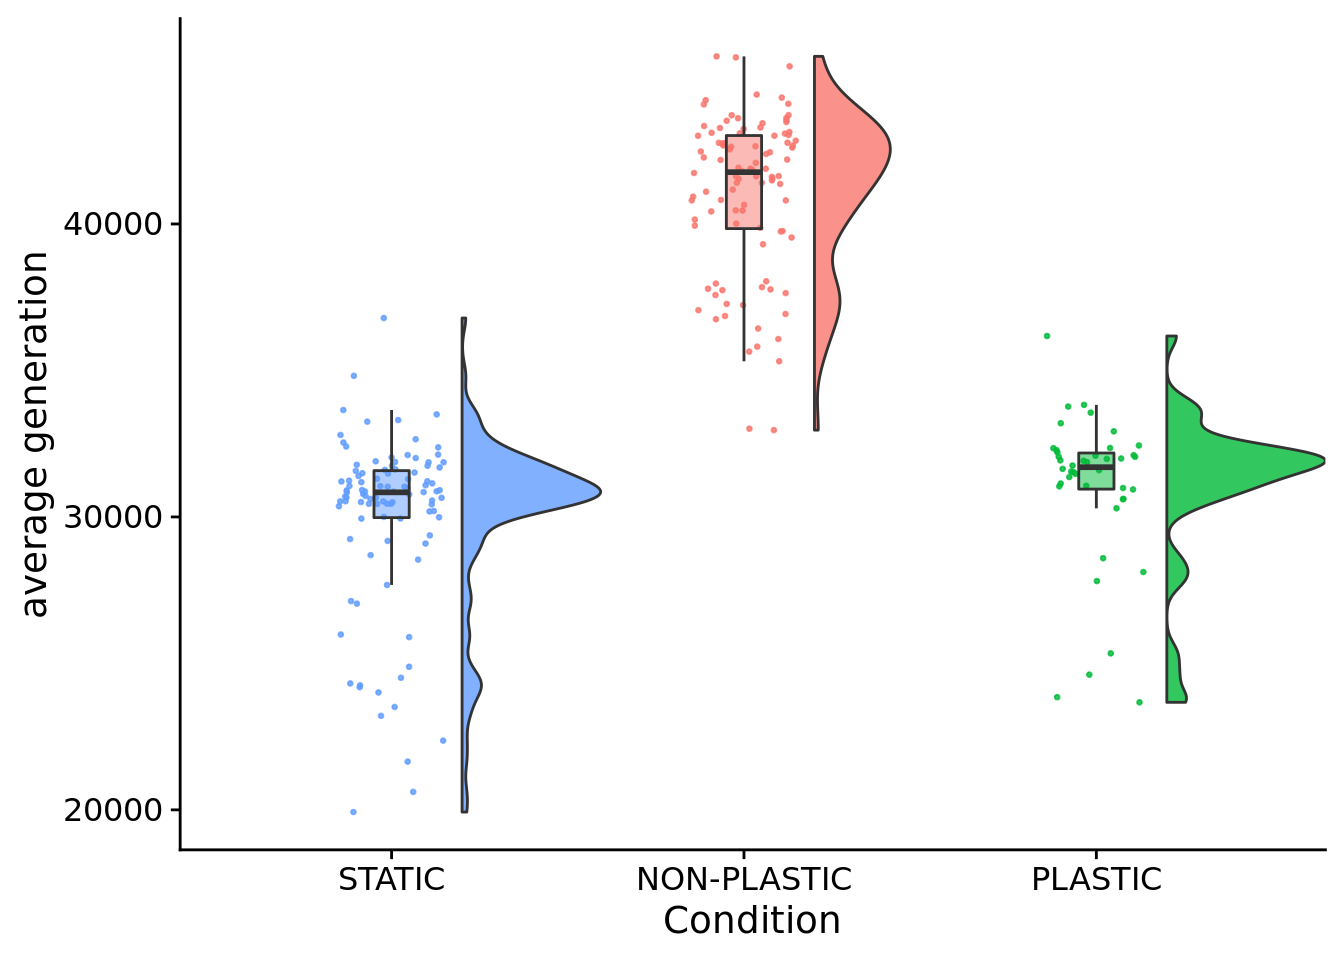
\includegraphics{supplemental-material_files/figure-latex/unnamed-chunk-13-1.pdf}

\begin{Shaded}
\begin{Highlighting}[]
\KeywordTok{paste0}\NormalTok{(}
  \StringTok{"PLASTIC median: "}\NormalTok{,}
  \KeywordTok{median}\NormalTok{(}\KeywordTok{filter}\NormalTok{(summary_data, condition}\OperatorTok{==}\StringTok{"PLASTIC"}\NormalTok{)}\OperatorTok{$}\NormalTok{time_average_generation)}
\NormalTok{)}
\end{Highlighting}
\end{Shaded}

\begin{verbatim}
## [1] "PLASTIC median: 31697.65"
\end{verbatim}

\begin{Shaded}
\begin{Highlighting}[]
\KeywordTok{paste0}\NormalTok{(}
  \StringTok{"STATIC median: "}\NormalTok{,}
  \KeywordTok{median}\NormalTok{(}\KeywordTok{filter}\NormalTok{(summary_data, condition}\OperatorTok{==}\StringTok{"STATIC"}\NormalTok{)}\OperatorTok{$}\NormalTok{time_average_generation)}
\NormalTok{)}
\end{Highlighting}
\end{Shaded}

\begin{verbatim}
## [1] "STATIC median: 30839.75"
\end{verbatim}

\begin{Shaded}
\begin{Highlighting}[]
\KeywordTok{paste0}\NormalTok{(}
  \StringTok{"NON-PLASTIC median: "}\NormalTok{,}
  \KeywordTok{median}\NormalTok{(}\KeywordTok{filter}\NormalTok{(summary_data, condition}\OperatorTok{==}\StringTok{"NON-PLASTIC"}\NormalTok{)}\OperatorTok{$}\NormalTok{time_average_generation)}
\NormalTok{)}
\end{Highlighting}
\end{Shaded}

\begin{verbatim}
## [1] "NON-PLASTIC median: 41768.65"
\end{verbatim}

\begin{Shaded}
\begin{Highlighting}[]
\KeywordTok{kruskal.test}\NormalTok{(}
  \DataTypeTok{formula=}\NormalTok{time_average_generation}\OperatorTok{~}\NormalTok{condition,}
  \DataTypeTok{data=}\NormalTok{summary_data}
\NormalTok{)}
\end{Highlighting}
\end{Shaded}

\begin{verbatim}
## 
##  Kruskal-Wallis rank sum test
## 
## data:  time_average_generation by condition
## Kruskal-Wallis chi-squared = 177.33, df = 2, p-value < 2.2e-16
\end{verbatim}

\begin{Shaded}
\begin{Highlighting}[]
\KeywordTok{pairwise.wilcox.test}\NormalTok{(}
  \DataTypeTok{x=}\NormalTok{summary_data}\OperatorTok{$}\NormalTok{time_average_generation,}
  \DataTypeTok{g=}\NormalTok{summary_data}\OperatorTok{$}\NormalTok{condition,}
  \DataTypeTok{p.adjust.method=}\StringTok{"bonferroni"}\NormalTok{,}
\NormalTok{)}
\end{Highlighting}
\end{Shaded}

\begin{verbatim}
## 
##  Pairwise comparisons using Wilcoxon rank sum test with continuity correction 
## 
## data:  summary_data$time_average_generation and summary_data$condition 
## 
##         NON-PLASTIC PLASTIC
## PLASTIC <2e-16      -      
## STATIC  <2e-16      0.004  
## 
## P value adjustment method: bonferroni
\end{verbatim}

\hypertarget{selective-sweeps}{%
\section{Selective sweeps}\label{selective-sweeps}}

The number of times the most recent common ancestor changes gives us the number of selective sweeps that occur during the experiment.

\begin{Shaded}
\begin{Highlighting}[]
\KeywordTok{ggplot}\NormalTok{(summary_data, }\KeywordTok{aes}\NormalTok{(}\DataTypeTok{x=}\NormalTok{condition, }\DataTypeTok{y=}\NormalTok{phylo_mrca_changes, }\DataTypeTok{fill=}\NormalTok{condition)) }\OperatorTok{+}
\StringTok{  }\KeywordTok{geom_flat_violin}\NormalTok{(}
    \DataTypeTok{position =} \KeywordTok{position_nudge}\NormalTok{(}\DataTypeTok{x =} \FloatTok{.2}\NormalTok{, }\DataTypeTok{y =} \DecValTok{0}\NormalTok{),}
    \DataTypeTok{alpha =} \FloatTok{.8}
\NormalTok{  ) }\OperatorTok{+}
\StringTok{  }\KeywordTok{geom_point}\NormalTok{(}
    \DataTypeTok{mapping=}\KeywordTok{aes}\NormalTok{(}\DataTypeTok{color=}\NormalTok{condition),}
    \DataTypeTok{position =} \KeywordTok{position_jitter}\NormalTok{(}\DataTypeTok{width =} \FloatTok{.15}\NormalTok{),}
    \DataTypeTok{size =} \FloatTok{.5}\NormalTok{,}
    \DataTypeTok{alpha =} \FloatTok{0.8}
\NormalTok{  ) }\OperatorTok{+}
\StringTok{  }\KeywordTok{geom_boxplot}\NormalTok{(}
    \DataTypeTok{width =} \FloatTok{.1}\NormalTok{,}
    \DataTypeTok{outlier.shape =} \OtherTok{NA}\NormalTok{,}
    \DataTypeTok{alpha =} \FloatTok{0.5}
\NormalTok{  ) }\OperatorTok{+}
\StringTok{  }\KeywordTok{scale_x_discrete}\NormalTok{(}
    \DataTypeTok{name=}\StringTok{"Condition"}\NormalTok{,}
    \DataTypeTok{limits=}\NormalTok{condition_order}
\NormalTok{  ) }\OperatorTok{+}
\StringTok{  }\KeywordTok{ylab}\NormalTok{(}\StringTok{"Number of selective sweeps"}\NormalTok{) }\OperatorTok{+}
\StringTok{  }\KeywordTok{theme}\NormalTok{(}
    \DataTypeTok{legend.position=}\StringTok{"none"}
\NormalTok{  )}
\end{Highlighting}
\end{Shaded}

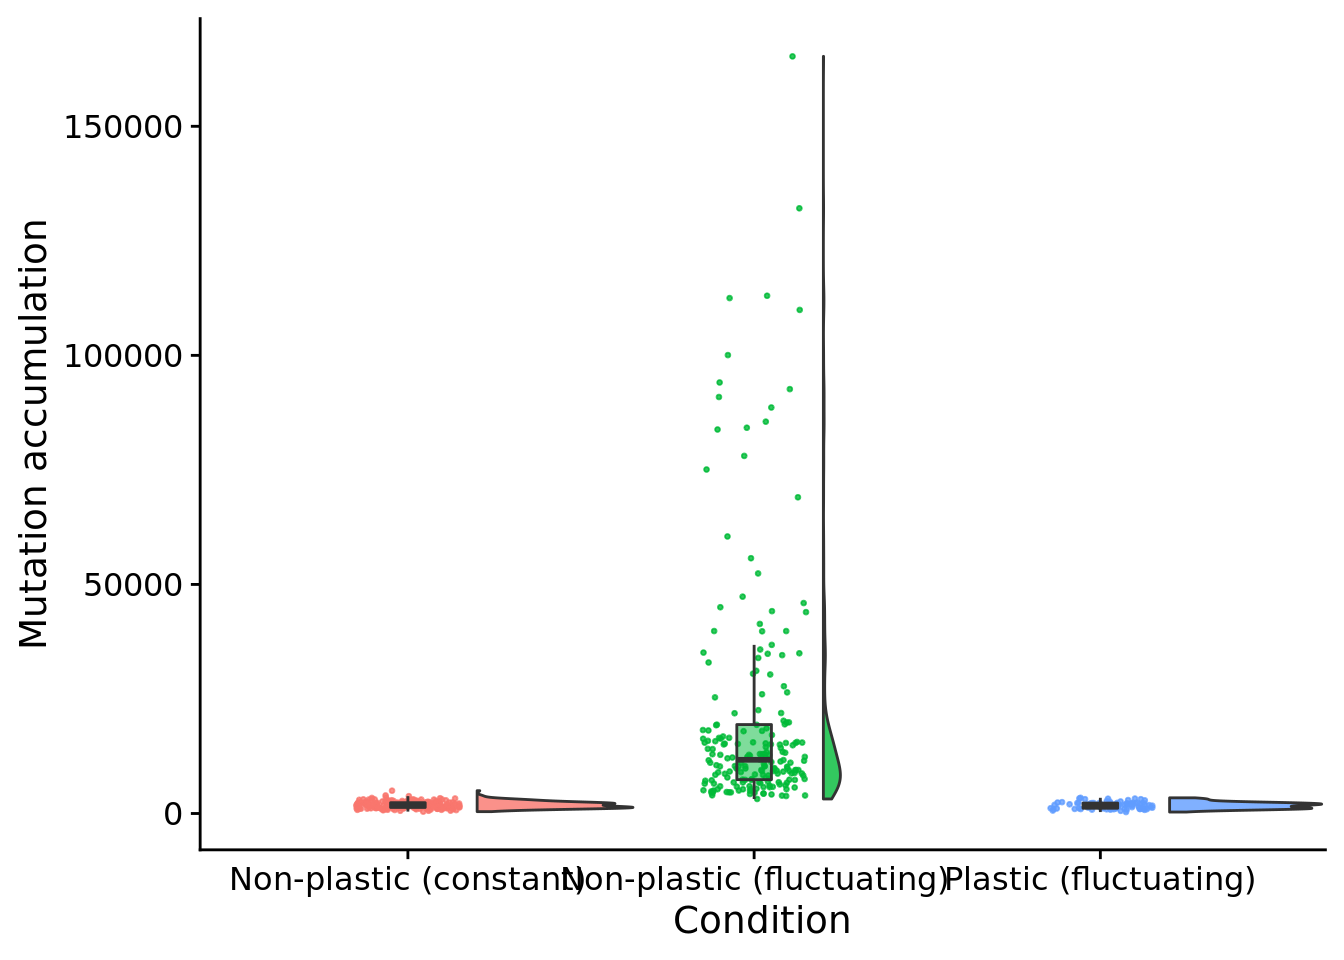
\includegraphics{supplemental-material_files/figure-latex/unnamed-chunk-15-1.pdf}

\begin{Shaded}
\begin{Highlighting}[]
\KeywordTok{paste0}\NormalTok{(}
  \StringTok{"PLASTIC: "}\NormalTok{,}
  \KeywordTok{median}\NormalTok{(}\KeywordTok{filter}\NormalTok{(summary_data, condition}\OperatorTok{==}\StringTok{"PLASTIC"}\NormalTok{)}\OperatorTok{$}\NormalTok{phylo_mrca_changes)}
\NormalTok{)}
\end{Highlighting}
\end{Shaded}

\begin{verbatim}
## [1] "PLASTIC: 45.5"
\end{verbatim}

\begin{Shaded}
\begin{Highlighting}[]
\KeywordTok{paste0}\NormalTok{(}
  \StringTok{"STATIC: "}\NormalTok{,}
  \KeywordTok{median}\NormalTok{(}\KeywordTok{filter}\NormalTok{(summary_data, condition}\OperatorTok{==}\StringTok{"STATIC"}\NormalTok{)}\OperatorTok{$}\NormalTok{phylo_mrca_changes)}
\NormalTok{)}
\end{Highlighting}
\end{Shaded}

\begin{verbatim}
## [1] "STATIC: 45"
\end{verbatim}

\begin{Shaded}
\begin{Highlighting}[]
\KeywordTok{paste0}\NormalTok{(}
  \StringTok{"NON-PLASTIC: "}\NormalTok{,}
  \KeywordTok{median}\NormalTok{(}\KeywordTok{filter}\NormalTok{(summary_data, condition}\OperatorTok{==}\StringTok{"NON-PLASTIC"}\NormalTok{)}\OperatorTok{$}\NormalTok{phylo_mrca_changes)}
\NormalTok{)}
\end{Highlighting}
\end{Shaded}

\begin{verbatim}
## [1] "NON-PLASTIC: 663.5"
\end{verbatim}

\begin{Shaded}
\begin{Highlighting}[]
\KeywordTok{kruskal.test}\NormalTok{(}
  \DataTypeTok{formula=}\NormalTok{phylo_mrca_changes}\OperatorTok{~}\NormalTok{condition,}
  \DataTypeTok{data=}\NormalTok{summary_data}
\NormalTok{)}
\end{Highlighting}
\end{Shaded}

\begin{verbatim}
## 
##  Kruskal-Wallis rank sum test
## 
## data:  phylo_mrca_changes by condition
## Kruskal-Wallis chi-squared = 175.46, df = 2, p-value < 2.2e-16
\end{verbatim}

\begin{Shaded}
\begin{Highlighting}[]
\KeywordTok{pairwise.wilcox.test}\NormalTok{(}
  \DataTypeTok{x=}\NormalTok{summary_data}\OperatorTok{$}\NormalTok{phylo_mrca_changes,}
  \DataTypeTok{g=}\NormalTok{summary_data}\OperatorTok{$}\NormalTok{condition,}
  \DataTypeTok{p.adjust.method=}\StringTok{"bonferroni"}\NormalTok{,}
\NormalTok{)}
\end{Highlighting}
\end{Shaded}

\begin{verbatim}
## 
##  Pairwise comparisons using Wilcoxon rank sum test with continuity correction 
## 
## data:  summary_data$phylo_mrca_changes and summary_data$condition 
## 
##         NON-PLASTIC PLASTIC
## PLASTIC <2e-16      -      
## STATIC  <2e-16      1      
## 
## P value adjustment method: bonferroni
\end{verbatim}

\hypertarget{average-number-of-generations-between-selective-sweeps}{%
\subsection{Average number of generations between selective sweeps}\label{average-number-of-generations-between-selective-sweeps}}

\begin{Shaded}
\begin{Highlighting}[]
\NormalTok{summary_data}\OperatorTok{$}\NormalTok{generations_per_mrca_change <-}\StringTok{ }\NormalTok{summary_data}\OperatorTok{$}\NormalTok{time_average_generation }\OperatorTok{/}\StringTok{ }\NormalTok{summary_data}\OperatorTok{$}\NormalTok{phylo_mrca_changes}

\KeywordTok{ggplot}\NormalTok{(summary_data, }\KeywordTok{aes}\NormalTok{(}\DataTypeTok{x=}\NormalTok{condition, }\DataTypeTok{y=}\NormalTok{generations_per_mrca_change, }\DataTypeTok{fill=}\NormalTok{condition)) }\OperatorTok{+}
\StringTok{  }\KeywordTok{geom_flat_violin}\NormalTok{(}
    \DataTypeTok{position =} \KeywordTok{position_nudge}\NormalTok{(}\DataTypeTok{x =} \FloatTok{.2}\NormalTok{, }\DataTypeTok{y =} \DecValTok{0}\NormalTok{),}
    \DataTypeTok{alpha =} \FloatTok{.8}
\NormalTok{  ) }\OperatorTok{+}
\StringTok{  }\KeywordTok{geom_point}\NormalTok{(}
    \DataTypeTok{mapping=}\KeywordTok{aes}\NormalTok{(}\DataTypeTok{color=}\NormalTok{condition),}
    \DataTypeTok{position =} \KeywordTok{position_jitter}\NormalTok{(}\DataTypeTok{width =} \FloatTok{.15}\NormalTok{),}
    \DataTypeTok{size =} \FloatTok{.5}\NormalTok{,}
    \DataTypeTok{alpha =} \FloatTok{0.8}
\NormalTok{  ) }\OperatorTok{+}
\StringTok{  }\KeywordTok{geom_boxplot}\NormalTok{(}
    \DataTypeTok{width =} \FloatTok{.1}\NormalTok{,}
    \DataTypeTok{outlier.shape =} \OtherTok{NA}\NormalTok{,}
    \DataTypeTok{alpha =} \FloatTok{0.5}
\NormalTok{  ) }\OperatorTok{+}
\StringTok{  }\KeywordTok{scale_x_discrete}\NormalTok{(}
    \DataTypeTok{name=}\StringTok{"Condition"}\NormalTok{,}
    \DataTypeTok{limits=}\NormalTok{condition_order}
\NormalTok{  ) }\OperatorTok{+}
\StringTok{  }\KeywordTok{theme}\NormalTok{(}
    \DataTypeTok{legend.position=}\StringTok{"none"}
\NormalTok{  )}
\end{Highlighting}
\end{Shaded}

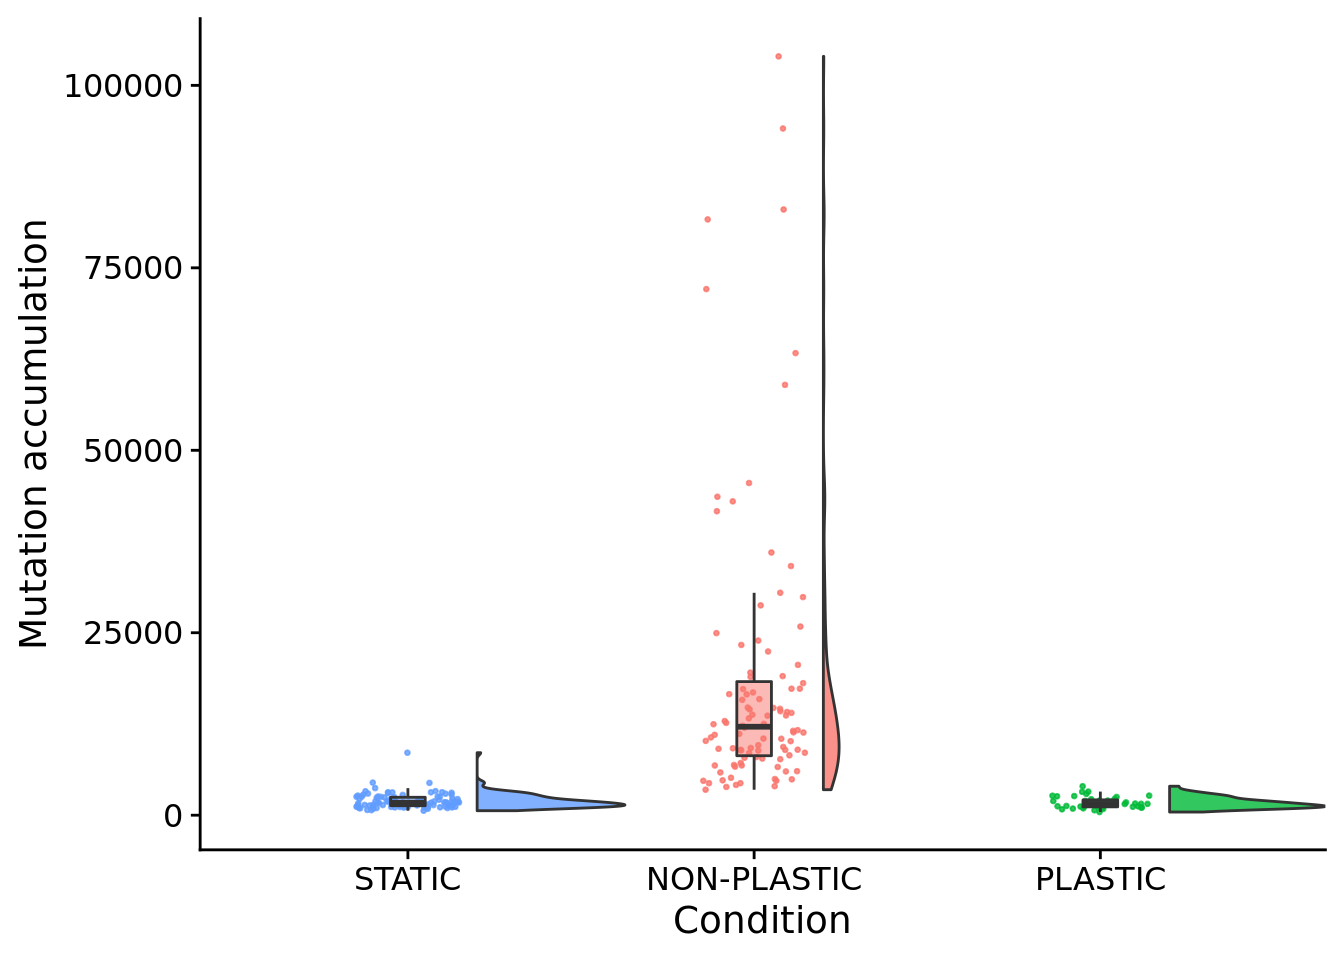
\includegraphics{supplemental-material_files/figure-latex/unnamed-chunk-17-1.pdf}

\begin{Shaded}
\begin{Highlighting}[]
\KeywordTok{paste0}\NormalTok{(}
  \StringTok{"PLASTIC: "}\NormalTok{,}
  \KeywordTok{median}\NormalTok{(}\KeywordTok{filter}\NormalTok{(summary_data, condition}\OperatorTok{==}\StringTok{"PLASTIC"}\NormalTok{)}\OperatorTok{$}\NormalTok{generations_per_mrca_change)}
\NormalTok{)}
\end{Highlighting}
\end{Shaded}

\begin{verbatim}
## [1] "PLASTIC: 685.001780758557"
\end{verbatim}

\begin{Shaded}
\begin{Highlighting}[]
\KeywordTok{paste0}\NormalTok{(}
  \StringTok{"STATIC: "}\NormalTok{,}
  \KeywordTok{median}\NormalTok{(}\KeywordTok{filter}\NormalTok{(summary_data, condition}\OperatorTok{==}\StringTok{"STATIC"}\NormalTok{)}\OperatorTok{$}\NormalTok{generations_per_mrca_change)}
\NormalTok{)}
\end{Highlighting}
\end{Shaded}

\begin{verbatim}
## [1] "STATIC: 693.676265008576"
\end{verbatim}

\begin{Shaded}
\begin{Highlighting}[]
\KeywordTok{paste0}\NormalTok{(}
  \StringTok{"NON-PLASTIC: "}\NormalTok{,}
  \KeywordTok{median}\NormalTok{(}\KeywordTok{filter}\NormalTok{(summary_data, condition}\OperatorTok{==}\StringTok{"NON-PLASTIC"}\NormalTok{)}\OperatorTok{$}\NormalTok{generations_per_mrca_change)}
\NormalTok{)}
\end{Highlighting}
\end{Shaded}

\begin{verbatim}
## [1] "NON-PLASTIC: 62.0184902295191"
\end{verbatim}

\begin{Shaded}
\begin{Highlighting}[]
\KeywordTok{kruskal.test}\NormalTok{(}
  \DataTypeTok{formula=}\NormalTok{generations_per_mrca_change}\OperatorTok{~}\NormalTok{condition,}
  \DataTypeTok{data=}\NormalTok{summary_data}
\NormalTok{)}
\end{Highlighting}
\end{Shaded}

\begin{verbatim}
## 
##  Kruskal-Wallis rank sum test
## 
## data:  generations_per_mrca_change by condition
## Kruskal-Wallis chi-squared = 175.33, df = 2, p-value < 2.2e-16
\end{verbatim}

\begin{Shaded}
\begin{Highlighting}[]
\KeywordTok{pairwise.wilcox.test}\NormalTok{(}
  \DataTypeTok{x=}\NormalTok{summary_data}\OperatorTok{$}\NormalTok{generations_per_mrca_change,}
  \DataTypeTok{g=}\NormalTok{summary_data}\OperatorTok{$}\NormalTok{condition,}
  \DataTypeTok{p.adjust.method=}\StringTok{"bonferroni"}\NormalTok{,}
\NormalTok{)}
\end{Highlighting}
\end{Shaded}

\begin{verbatim}
## 
##  Pairwise comparisons using Wilcoxon rank sum test with continuity correction 
## 
## data:  summary_data$generations_per_mrca_change and summary_data$condition 
## 
##         NON-PLASTIC PLASTIC
## PLASTIC <2e-16      -      
## STATIC  <2e-16      1      
## 
## P value adjustment method: bonferroni
\end{verbatim}

\hypertarget{phenotypic-volatility-along-dominant-lineage}{%
\section{Phenotypic volatility along dominant lineage}\label{phenotypic-volatility-along-dominant-lineage}}

\begin{Shaded}
\begin{Highlighting}[]
\KeywordTok{ggplot}\NormalTok{(summary_data, }\KeywordTok{aes}\NormalTok{(}\DataTypeTok{x=}\NormalTok{condition, }\DataTypeTok{y=}\NormalTok{dominant_lineage_trait_volatility, }\DataTypeTok{fill=}\NormalTok{condition)) }\OperatorTok{+}
\StringTok{  }\KeywordTok{geom_flat_violin}\NormalTok{(}
    \DataTypeTok{position =} \KeywordTok{position_nudge}\NormalTok{(}\DataTypeTok{x =} \FloatTok{.2}\NormalTok{, }\DataTypeTok{y =} \DecValTok{0}\NormalTok{),}
    \DataTypeTok{alpha =} \FloatTok{.8}
\NormalTok{  ) }\OperatorTok{+}
\StringTok{  }\KeywordTok{geom_point}\NormalTok{(}
    \DataTypeTok{mapping=}\KeywordTok{aes}\NormalTok{(}\DataTypeTok{color=}\NormalTok{condition),}
    \DataTypeTok{position =} \KeywordTok{position_jitter}\NormalTok{(}\DataTypeTok{width =} \FloatTok{.15}\NormalTok{),}
    \DataTypeTok{size =} \FloatTok{.5}\NormalTok{,}
    \DataTypeTok{alpha =} \FloatTok{0.8}
\NormalTok{  ) }\OperatorTok{+}
\StringTok{  }\KeywordTok{geom_boxplot}\NormalTok{(}
    \DataTypeTok{width =} \FloatTok{.1}\NormalTok{,}
    \DataTypeTok{outlier.shape =} \OtherTok{NA}\NormalTok{,}
    \DataTypeTok{alpha =} \FloatTok{0.5}
\NormalTok{  ) }\OperatorTok{+}
\StringTok{  }\KeywordTok{scale_x_discrete}\NormalTok{(}
    \DataTypeTok{name=}\StringTok{"Condition"}\NormalTok{,}
    \DataTypeTok{limits=}\NormalTok{condition_order}
\NormalTok{  ) }\OperatorTok{+}
\StringTok{  }\KeywordTok{scale_y_continuous}\NormalTok{(}
    \DataTypeTok{name=}\StringTok{"Phenotypic volatility (log scale)"}\NormalTok{,}
    \DataTypeTok{trans=}\StringTok{"pseudo_log"}\NormalTok{,}
    \DataTypeTok{breaks=}\KeywordTok{c}\NormalTok{(}\DecValTok{0}\NormalTok{, }\DecValTok{10}\NormalTok{, }\DecValTok{100}\NormalTok{, }\DecValTok{1000}\NormalTok{, }\DecValTok{10000}\NormalTok{),}
    \DataTypeTok{limits=}\KeywordTok{c}\NormalTok{(}\OperatorTok{-}\DecValTok{1}\NormalTok{,}\DecValTok{10000}\NormalTok{)}
\NormalTok{  ) }\OperatorTok{+}
\StringTok{  }\KeywordTok{theme}\NormalTok{(}
    \DataTypeTok{legend.position=}\StringTok{"none"}
\NormalTok{  )}
\end{Highlighting}
\end{Shaded}

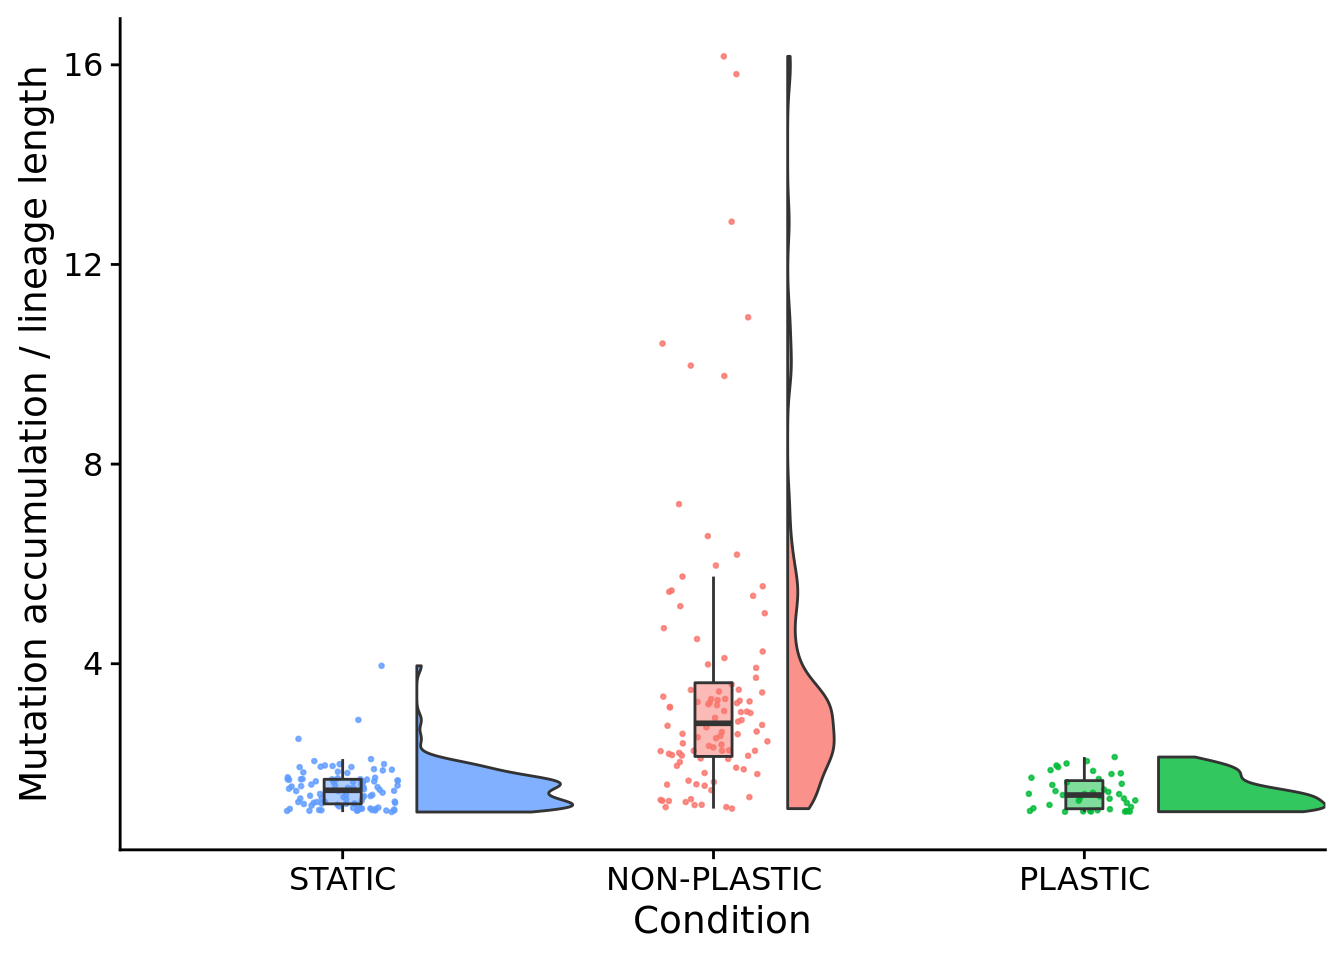
\includegraphics{supplemental-material_files/figure-latex/unnamed-chunk-19-1.pdf}

\begin{Shaded}
\begin{Highlighting}[]
\KeywordTok{paste0}\NormalTok{(}
  \StringTok{"PLASTIC: "}\NormalTok{,}
  \KeywordTok{median}\NormalTok{(}\KeywordTok{filter}\NormalTok{(summary_data, condition}\OperatorTok{==}\StringTok{"PLASTIC"}\NormalTok{)}\OperatorTok{$}\NormalTok{dominant_lineage_trait_volatility)}
\NormalTok{)}
\end{Highlighting}
\end{Shaded}

\begin{verbatim}
## [1] "PLASTIC: 2"
\end{verbatim}

\begin{Shaded}
\begin{Highlighting}[]
\KeywordTok{paste0}\NormalTok{(}
  \StringTok{"STATIC: "}\NormalTok{,}
  \KeywordTok{median}\NormalTok{(}\KeywordTok{filter}\NormalTok{(summary_data, condition}\OperatorTok{==}\StringTok{"STATIC"}\NormalTok{)}\OperatorTok{$}\NormalTok{dominant_lineage_trait_volatility)}
\NormalTok{)}
\end{Highlighting}
\end{Shaded}

\begin{verbatim}
## [1] "STATIC: 0"
\end{verbatim}

\begin{Shaded}
\begin{Highlighting}[]
\KeywordTok{paste0}\NormalTok{(}
  \StringTok{"NON-PLASTIC: "}\NormalTok{,}
  \KeywordTok{median}\NormalTok{(}\KeywordTok{filter}\NormalTok{(summary_data, condition}\OperatorTok{==}\StringTok{"NON-PLASTIC"}\NormalTok{)}\OperatorTok{$}\NormalTok{dominant_lineage_trait_volatility)}
\NormalTok{)}
\end{Highlighting}
\end{Shaded}

\begin{verbatim}
## [1] "NON-PLASTIC: 1868"
\end{verbatim}

\begin{Shaded}
\begin{Highlighting}[]
\KeywordTok{kruskal.test}\NormalTok{(}
  \DataTypeTok{formula=}\NormalTok{dominant_lineage_trait_volatility}\OperatorTok{~}\NormalTok{condition,}
  \DataTypeTok{data=}\NormalTok{summary_data}
\NormalTok{)}
\end{Highlighting}
\end{Shaded}

\begin{verbatim}
## 
##  Kruskal-Wallis rank sum test
## 
## data:  dominant_lineage_trait_volatility by condition
## Kruskal-Wallis chi-squared = 190.78, df = 2, p-value < 2.2e-16
\end{verbatim}

\begin{Shaded}
\begin{Highlighting}[]
\KeywordTok{pairwise.wilcox.test}\NormalTok{(}
  \DataTypeTok{x=}\NormalTok{summary_data}\OperatorTok{$}\NormalTok{dominant_lineage_trait_volatility,}
  \DataTypeTok{g=}\NormalTok{summary_data}\OperatorTok{$}\NormalTok{condition,}
  \DataTypeTok{p.adjust.method=}\StringTok{"bonferroni"}\NormalTok{,}
\NormalTok{)}
\end{Highlighting}
\end{Shaded}

\begin{verbatim}
## 
##  Pairwise comparisons using Wilcoxon rank sum test with continuity correction 
## 
## data:  summary_data$dominant_lineage_trait_volatility and summary_data$condition 
## 
##         NON-PLASTIC PLASTIC
## PLASTIC < 2e-16     -      
## STATIC  < 2e-16     8.7e-07
## 
## P value adjustment method: bonferroni
\end{verbatim}

\hypertarget{phenotypic-volatility-normalized-by-generations-elapsed}{%
\subsection{Phenotypic volatility normalized by generations elapsed}\label{phenotypic-volatility-normalized-by-generations-elapsed}}

\begin{Shaded}
\begin{Highlighting}[]
\NormalTok{summary_data}\OperatorTok{$}\NormalTok{dominant_lineage_trait_volatility_per_generation <-}\StringTok{ }\NormalTok{summary_data}\OperatorTok{$}\NormalTok{dominant_lineage_trait_volatility }\OperatorTok{/}\StringTok{ }\NormalTok{summary_data}\OperatorTok{$}\NormalTok{dominant_generation_born}

\KeywordTok{ggplot}\NormalTok{(summary_data, }\KeywordTok{aes}\NormalTok{(}\DataTypeTok{x=}\NormalTok{condition, }\DataTypeTok{y=}\NormalTok{dominant_lineage_trait_volatility_per_generation, }\DataTypeTok{fill=}\NormalTok{condition)) }\OperatorTok{+}
\StringTok{  }\KeywordTok{geom_flat_violin}\NormalTok{(}
    \DataTypeTok{position =} \KeywordTok{position_nudge}\NormalTok{(}\DataTypeTok{x =} \FloatTok{.2}\NormalTok{, }\DataTypeTok{y =} \DecValTok{0}\NormalTok{),}
    \DataTypeTok{alpha =} \FloatTok{.8}
\NormalTok{  ) }\OperatorTok{+}
\StringTok{  }\KeywordTok{geom_point}\NormalTok{(}
    \DataTypeTok{mapping=}\KeywordTok{aes}\NormalTok{(}\DataTypeTok{color=}\NormalTok{condition),}
    \DataTypeTok{position =} \KeywordTok{position_jitter}\NormalTok{(}\DataTypeTok{width =} \FloatTok{.15}\NormalTok{),}
    \DataTypeTok{size =} \FloatTok{.5}\NormalTok{,}
    \DataTypeTok{alpha =} \FloatTok{0.8}
\NormalTok{  ) }\OperatorTok{+}
\StringTok{  }\KeywordTok{geom_boxplot}\NormalTok{(}
    \DataTypeTok{width =} \FloatTok{.1}\NormalTok{,}
    \DataTypeTok{outlier.shape =} \OtherTok{NA}\NormalTok{,}
    \DataTypeTok{alpha =} \FloatTok{0.5}
\NormalTok{  ) }\OperatorTok{+}
\StringTok{  }\KeywordTok{scale_x_discrete}\NormalTok{(}
    \DataTypeTok{name=}\StringTok{"Condition"}\NormalTok{,}
    \DataTypeTok{limits=}\NormalTok{condition_order}
\NormalTok{  ) }\OperatorTok{+}
\StringTok{  }\KeywordTok{theme}\NormalTok{(}
    \DataTypeTok{legend.position=}\StringTok{"none"}
\NormalTok{  )}
\end{Highlighting}
\end{Shaded}

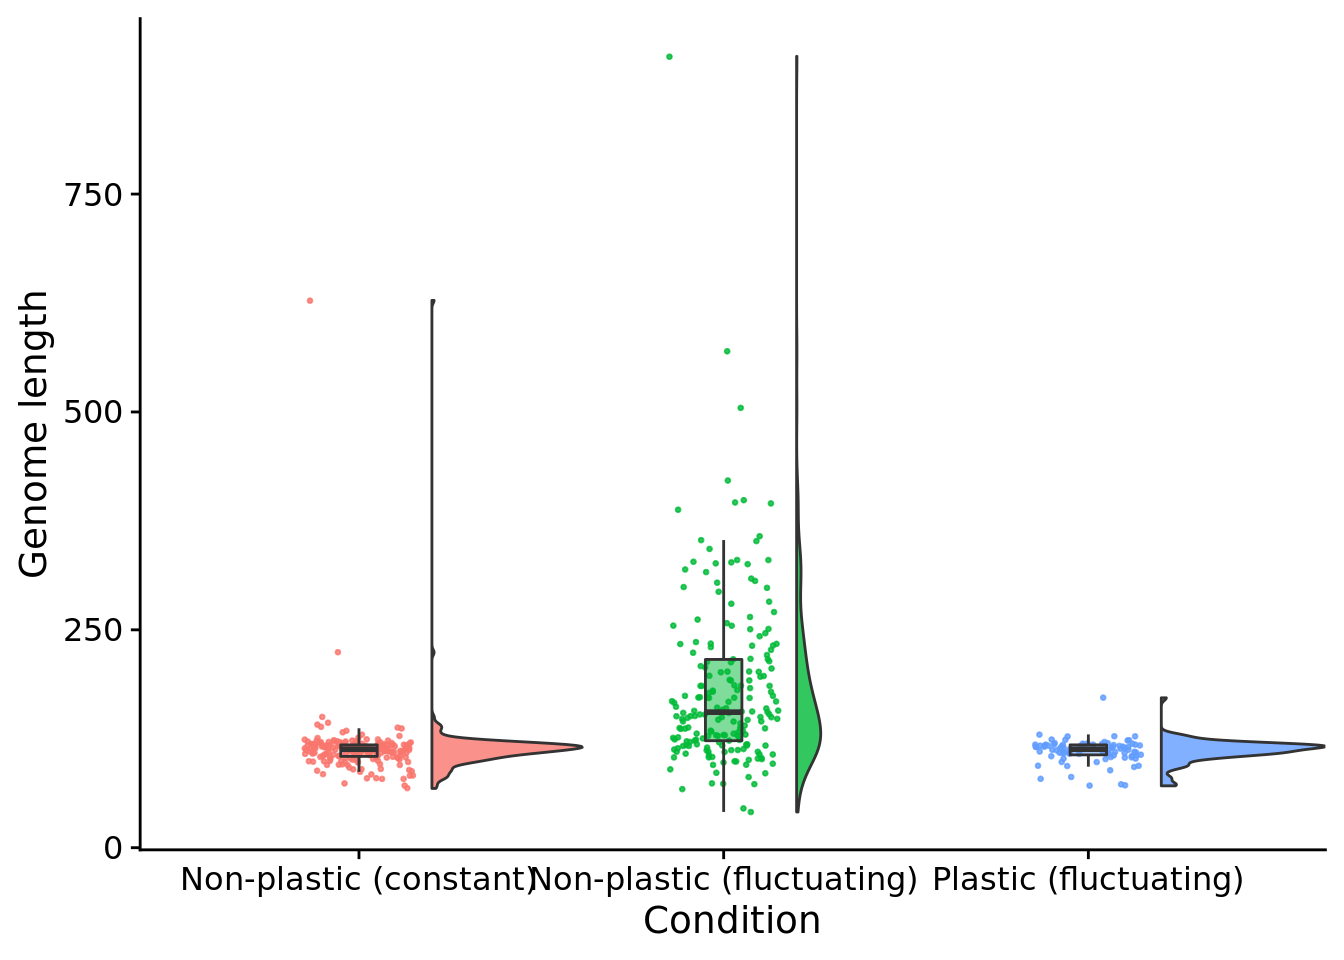
\includegraphics{supplemental-material_files/figure-latex/unnamed-chunk-21-1.pdf}

\begin{Shaded}
\begin{Highlighting}[]
\KeywordTok{paste0}\NormalTok{(}
  \StringTok{"PLASTIC: "}\NormalTok{,}
  \KeywordTok{median}\NormalTok{(}\KeywordTok{filter}\NormalTok{(summary_data, condition}\OperatorTok{==}\StringTok{"PLASTIC"}\NormalTok{)}\OperatorTok{$}\NormalTok{dominant_lineage_trait_volatility_per_generation)}
\NormalTok{)}
\end{Highlighting}
\end{Shaded}

\begin{verbatim}
## [1] "PLASTIC: 6.33339279717772e-05"
\end{verbatim}

\begin{Shaded}
\begin{Highlighting}[]
\KeywordTok{paste0}\NormalTok{(}
  \StringTok{"STATIC: "}\NormalTok{,}
  \KeywordTok{median}\NormalTok{(}\KeywordTok{filter}\NormalTok{(summary_data, condition}\OperatorTok{==}\StringTok{"STATIC"}\NormalTok{)}\OperatorTok{$}\NormalTok{dominant_lineage_trait_volatility_per_generation)}
\NormalTok{)}
\end{Highlighting}
\end{Shaded}

\begin{verbatim}
## [1] "STATIC: 0"
\end{verbatim}

\begin{Shaded}
\begin{Highlighting}[]
\KeywordTok{paste0}\NormalTok{(}
  \StringTok{"NON-PLASTIC: "}\NormalTok{,}
  \KeywordTok{median}\NormalTok{(}\KeywordTok{filter}\NormalTok{(summary_data, condition}\OperatorTok{==}\StringTok{"NON-PLASTIC"}\NormalTok{)}\OperatorTok{$}\NormalTok{dominant_lineage_trait_volatility_per_generation)}
\NormalTok{)}
\end{Highlighting}
\end{Shaded}

\begin{verbatim}
## [1] "NON-PLASTIC: 0.0447440145638177"
\end{verbatim}

\begin{Shaded}
\begin{Highlighting}[]
\KeywordTok{kruskal.test}\NormalTok{(}
  \DataTypeTok{formula=}\NormalTok{dominant_lineage_trait_volatility_per_generation}\OperatorTok{~}\NormalTok{condition,}
  \DataTypeTok{data=}\NormalTok{summary_data}
\NormalTok{)}
\end{Highlighting}
\end{Shaded}

\begin{verbatim}
## 
##  Kruskal-Wallis rank sum test
## 
## data:  dominant_lineage_trait_volatility_per_generation by condition
## Kruskal-Wallis chi-squared = 189.62, df = 2, p-value < 2.2e-16
\end{verbatim}

\begin{Shaded}
\begin{Highlighting}[]
\KeywordTok{pairwise.wilcox.test}\NormalTok{(}
  \DataTypeTok{x=}\NormalTok{summary_data}\OperatorTok{$}\NormalTok{dominant_lineage_trait_volatility_per_generation,}
  \DataTypeTok{g=}\NormalTok{summary_data}\OperatorTok{$}\NormalTok{condition,}
  \DataTypeTok{p.adjust.method=}\StringTok{"bonferroni"}\NormalTok{,}
\NormalTok{)}
\end{Highlighting}
\end{Shaded}

\begin{verbatim}
## 
##  Pairwise comparisons using Wilcoxon rank sum test with continuity correction 
## 
## data:  summary_data$dominant_lineage_trait_volatility_per_generation and summary_data$condition 
## 
##         NON-PLASTIC PLASTIC
## PLASTIC < 2e-16     -      
## STATIC  < 2e-16     4.2e-06
## 
## P value adjustment method: bonferroni
\end{verbatim}

\hypertarget{phenotypic-volatility-normalized-by-lineage-length}{%
\subsection{Phenotypic volatility normalized by lineage length}\label{phenotypic-volatility-normalized-by-lineage-length}}

Lineage length = number of genotypes along the lineage.

\begin{Shaded}
\begin{Highlighting}[]
\NormalTok{summary_data}\OperatorTok{$}\NormalTok{dominant_lineage_trait_volatility_per_lineage_step <-}\StringTok{ }\NormalTok{summary_data}\OperatorTok{$}\NormalTok{dominant_lineage_trait_volatility }\OperatorTok{/}\StringTok{ }\NormalTok{summary_data}\OperatorTok{$}\NormalTok{dominant_lineage_length_genotypes}

\KeywordTok{ggplot}\NormalTok{(summary_data, }\KeywordTok{aes}\NormalTok{(}\DataTypeTok{x=}\NormalTok{condition, }\DataTypeTok{y=}\NormalTok{dominant_lineage_trait_volatility_per_lineage_step, }\DataTypeTok{fill=}\NormalTok{condition)) }\OperatorTok{+}
\StringTok{  }\KeywordTok{geom_flat_violin}\NormalTok{(}
    \DataTypeTok{position =} \KeywordTok{position_nudge}\NormalTok{(}\DataTypeTok{x =} \FloatTok{.2}\NormalTok{, }\DataTypeTok{y =} \DecValTok{0}\NormalTok{),}
    \DataTypeTok{alpha =} \FloatTok{.8}
\NormalTok{  ) }\OperatorTok{+}
\StringTok{  }\KeywordTok{geom_point}\NormalTok{(}
    \DataTypeTok{mapping=}\KeywordTok{aes}\NormalTok{(}\DataTypeTok{color=}\NormalTok{condition),}
    \DataTypeTok{position =} \KeywordTok{position_jitter}\NormalTok{(}\DataTypeTok{width =} \FloatTok{.15}\NormalTok{),}
    \DataTypeTok{size =} \FloatTok{.5}\NormalTok{,}
    \DataTypeTok{alpha =} \FloatTok{0.8}
\NormalTok{  ) }\OperatorTok{+}
\StringTok{  }\KeywordTok{geom_boxplot}\NormalTok{(}
    \DataTypeTok{width =} \FloatTok{.1}\NormalTok{,}
    \DataTypeTok{outlier.shape =} \OtherTok{NA}\NormalTok{,}
    \DataTypeTok{alpha =} \FloatTok{0.5}
\NormalTok{  ) }\OperatorTok{+}
\StringTok{  }\KeywordTok{scale_x_discrete}\NormalTok{(}
    \DataTypeTok{name=}\StringTok{"Condition"}\NormalTok{,}
    \DataTypeTok{limits=}\NormalTok{condition_order}
\NormalTok{  ) }\OperatorTok{+}
\StringTok{  }\KeywordTok{theme}\NormalTok{(}
    \DataTypeTok{legend.position=}\StringTok{"none"}
\NormalTok{  )}
\end{Highlighting}
\end{Shaded}

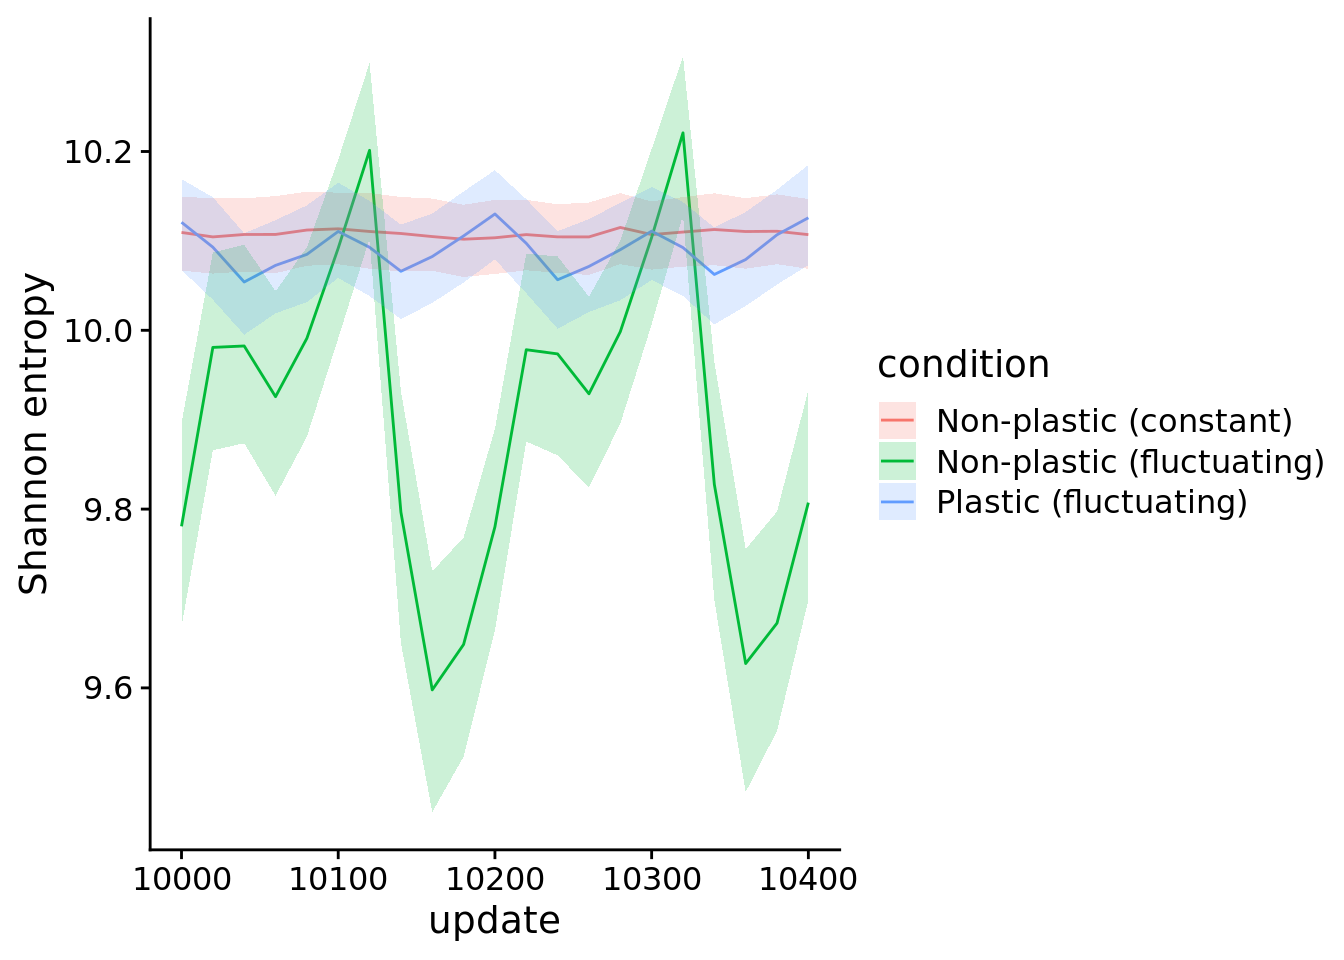
\includegraphics{supplemental-material_files/figure-latex/unnamed-chunk-23-1.pdf}

\begin{Shaded}
\begin{Highlighting}[]
\KeywordTok{paste0}\NormalTok{(}
  \StringTok{"PLASTIC: "}\NormalTok{,}
  \KeywordTok{median}\NormalTok{(}\KeywordTok{filter}\NormalTok{(summary_data, condition}\OperatorTok{==}\StringTok{"PLASTIC"}\NormalTok{)}\OperatorTok{$}\NormalTok{dominant_lineage_trait_volatility_per_lineage_step)}
\NormalTok{)}
\end{Highlighting}
\end{Shaded}

\begin{verbatim}
## [1] "PLASTIC: 0.00224688783339238"
\end{verbatim}

\begin{Shaded}
\begin{Highlighting}[]
\KeywordTok{paste0}\NormalTok{(}
  \StringTok{"STATIC: "}\NormalTok{,}
  \KeywordTok{median}\NormalTok{(}\KeywordTok{filter}\NormalTok{(summary_data, condition}\OperatorTok{==}\StringTok{"STATIC"}\NormalTok{)}\OperatorTok{$}\NormalTok{dominant_lineage_trait_volatility_per_lineage_step)}
\NormalTok{)}
\end{Highlighting}
\end{Shaded}

\begin{verbatim}
## [1] "STATIC: 0"
\end{verbatim}

\begin{Shaded}
\begin{Highlighting}[]
\KeywordTok{paste0}\NormalTok{(}
  \StringTok{"NON-PLASTIC: "}\NormalTok{,}
  \KeywordTok{median}\NormalTok{(}\KeywordTok{filter}\NormalTok{(summary_data, condition}\OperatorTok{==}\StringTok{"NON-PLASTIC"}\NormalTok{)}\OperatorTok{$}\NormalTok{dominant_lineage_trait_volatility_per_lineage_step)}
\NormalTok{)}
\end{Highlighting}
\end{Shaded}

\begin{verbatim}
## [1] "NON-PLASTIC: 0.437482522172625"
\end{verbatim}

\begin{Shaded}
\begin{Highlighting}[]
\KeywordTok{kruskal.test}\NormalTok{(}
  \DataTypeTok{formula=}\NormalTok{dominant_lineage_trait_volatility_per_lineage_step}\OperatorTok{~}\NormalTok{condition,}
  \DataTypeTok{data=}\NormalTok{summary_data}
\NormalTok{)}
\end{Highlighting}
\end{Shaded}

\begin{verbatim}
## 
##  Kruskal-Wallis rank sum test
## 
## data:  dominant_lineage_trait_volatility_per_lineage_step by condition
## Kruskal-Wallis chi-squared = 191.23, df = 2, p-value < 2.2e-16
\end{verbatim}

\begin{Shaded}
\begin{Highlighting}[]
\KeywordTok{pairwise.wilcox.test}\NormalTok{(}
  \DataTypeTok{x=}\NormalTok{summary_data}\OperatorTok{$}\NormalTok{dominant_lineage_trait_volatility_per_lineage_step,}
  \DataTypeTok{g=}\NormalTok{summary_data}\OperatorTok{$}\NormalTok{condition,}
  \DataTypeTok{p.adjust.method=}\StringTok{"bonferroni"}\NormalTok{,}
\NormalTok{)}
\end{Highlighting}
\end{Shaded}

\begin{verbatim}
## 
##  Pairwise comparisons using Wilcoxon rank sum test with continuity correction 
## 
## data:  summary_data$dominant_lineage_trait_volatility_per_lineage_step and summary_data$condition 
## 
##         NON-PLASTIC PLASTIC
## PLASTIC < 2e-16     -      
## STATIC  < 2e-16     2.3e-07
## 
## P value adjustment method: bonferroni
\end{verbatim}

\hypertarget{phenotypic-fidelity}{%
\subsection{Phenotypic fidelity}\label{phenotypic-fidelity}}

Frequency that an offspring's genotype is identical to a parent genotype (along the dominant lineage).

\begin{Shaded}
\begin{Highlighting}[]
\NormalTok{summary_data}\OperatorTok{$}\NormalTok{dominant_lineage_trait_fidelity <-}\StringTok{ }\NormalTok{(summary_data}\OperatorTok{$}\NormalTok{dominant_generation_born }\OperatorTok{-}\StringTok{ }\NormalTok{summary_data}\OperatorTok{$}\NormalTok{dominant_lineage_trait_volatility) }\OperatorTok{/}\StringTok{ }\NormalTok{summary_data}\OperatorTok{$}\NormalTok{dominant_generation_born}

\KeywordTok{ggplot}\NormalTok{(summary_data, }\KeywordTok{aes}\NormalTok{(}\DataTypeTok{x=}\NormalTok{condition, }\DataTypeTok{y=}\NormalTok{dominant_lineage_trait_fidelity, }\DataTypeTok{fill=}\NormalTok{condition)) }\OperatorTok{+}
\StringTok{  }\KeywordTok{geom_flat_violin}\NormalTok{(}
    \DataTypeTok{position =} \KeywordTok{position_nudge}\NormalTok{(}\DataTypeTok{x =} \FloatTok{.2}\NormalTok{, }\DataTypeTok{y =} \DecValTok{0}\NormalTok{),}
    \DataTypeTok{alpha =} \FloatTok{.8}
\NormalTok{  ) }\OperatorTok{+}
\StringTok{  }\KeywordTok{geom_point}\NormalTok{(}
    \DataTypeTok{mapping=}\KeywordTok{aes}\NormalTok{(}\DataTypeTok{color=}\NormalTok{condition),}
    \DataTypeTok{position =} \KeywordTok{position_jitter}\NormalTok{(}\DataTypeTok{width =} \FloatTok{.15}\NormalTok{),}
    \DataTypeTok{size =} \FloatTok{.5}\NormalTok{,}
    \DataTypeTok{alpha =} \FloatTok{0.8}
\NormalTok{  ) }\OperatorTok{+}
\StringTok{  }\KeywordTok{geom_boxplot}\NormalTok{(}
    \DataTypeTok{width =} \FloatTok{.1}\NormalTok{,}
    \DataTypeTok{outlier.shape =} \OtherTok{NA}\NormalTok{,}
    \DataTypeTok{alpha =} \FloatTok{0.5}
\NormalTok{  ) }\OperatorTok{+}
\StringTok{  }\KeywordTok{scale_x_discrete}\NormalTok{(}
    \DataTypeTok{name=}\StringTok{"Condition"}\NormalTok{,}
    \DataTypeTok{limits=}\NormalTok{condition_order}
\NormalTok{  ) }\OperatorTok{+}
\StringTok{  }\KeywordTok{theme}\NormalTok{(}
    \DataTypeTok{legend.position=}\StringTok{"none"}
\NormalTok{  )}
\end{Highlighting}
\end{Shaded}

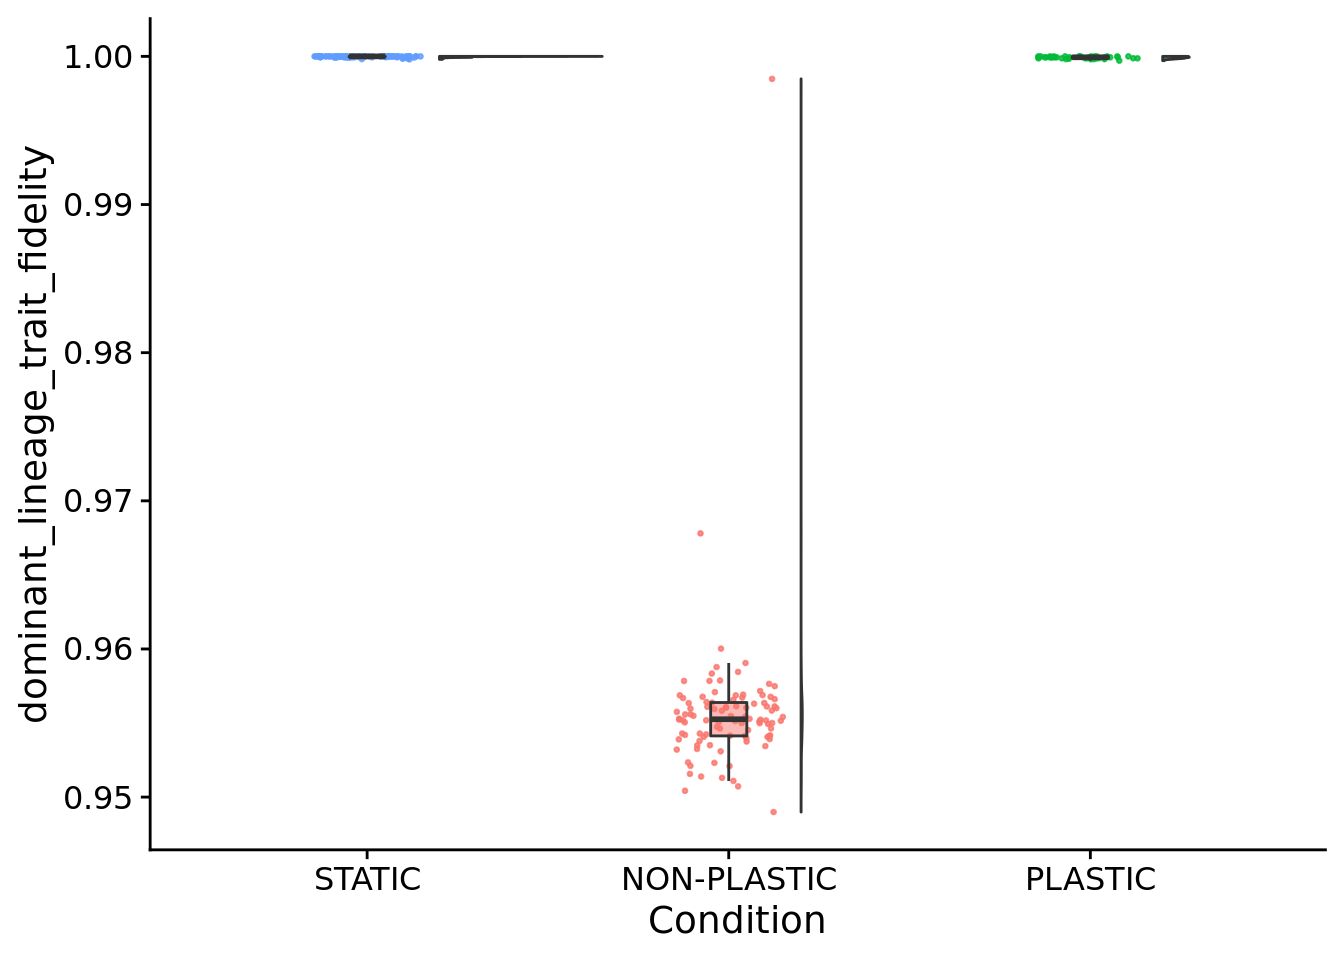
\includegraphics{supplemental-material_files/figure-latex/unnamed-chunk-25-1.pdf}

\begin{Shaded}
\begin{Highlighting}[]
\KeywordTok{paste0}\NormalTok{(}
  \StringTok{"PLASTIC: "}\NormalTok{,}
  \KeywordTok{median}\NormalTok{(}\KeywordTok{filter}\NormalTok{(summary_data, condition}\OperatorTok{==}\StringTok{"PLASTIC"}\NormalTok{)}\OperatorTok{$}\NormalTok{dominant_lineage_trait_fidelity)}
\NormalTok{)}
\end{Highlighting}
\end{Shaded}

\begin{verbatim}
## [1] "PLASTIC: 0.999936666072028"
\end{verbatim}

\begin{Shaded}
\begin{Highlighting}[]
\KeywordTok{paste0}\NormalTok{(}
  \StringTok{"STATIC: "}\NormalTok{,}
  \KeywordTok{median}\NormalTok{(}\KeywordTok{filter}\NormalTok{(summary_data, condition}\OperatorTok{==}\StringTok{"STATIC"}\NormalTok{)}\OperatorTok{$}\NormalTok{dominant_lineage_trait_fidelity)}
\NormalTok{)}
\end{Highlighting}
\end{Shaded}

\begin{verbatim}
## [1] "STATIC: 1"
\end{verbatim}

\begin{Shaded}
\begin{Highlighting}[]
\KeywordTok{paste0}\NormalTok{(}
  \StringTok{"NON-PLASTIC: "}\NormalTok{,}
  \KeywordTok{median}\NormalTok{(}\KeywordTok{filter}\NormalTok{(summary_data, condition}\OperatorTok{==}\StringTok{"NON-PLASTIC"}\NormalTok{)}\OperatorTok{$}\NormalTok{dominant_lineage_trait_fidelity)}
\NormalTok{)}
\end{Highlighting}
\end{Shaded}

\begin{verbatim}
## [1] "NON-PLASTIC: 0.955255985436182"
\end{verbatim}

\begin{Shaded}
\begin{Highlighting}[]
\KeywordTok{kruskal.test}\NormalTok{(}
  \DataTypeTok{formula=}\NormalTok{dominant_lineage_trait_fidelity}\OperatorTok{~}\NormalTok{condition,}
  \DataTypeTok{data=}\NormalTok{summary_data}
\NormalTok{)}
\end{Highlighting}
\end{Shaded}

\begin{verbatim}
## 
##  Kruskal-Wallis rank sum test
## 
## data:  dominant_lineage_trait_fidelity by condition
## Kruskal-Wallis chi-squared = 189.62, df = 2, p-value < 2.2e-16
\end{verbatim}

\begin{Shaded}
\begin{Highlighting}[]
\KeywordTok{pairwise.wilcox.test}\NormalTok{(}
  \DataTypeTok{x=}\NormalTok{summary_data}\OperatorTok{$}\NormalTok{dominant_lineage_trait_fidelity,}
  \DataTypeTok{g=}\NormalTok{summary_data}\OperatorTok{$}\NormalTok{condition,}
  \DataTypeTok{p.adjust.method=}\StringTok{"bonferroni"}\NormalTok{,}
\NormalTok{)}
\end{Highlighting}
\end{Shaded}

\begin{verbatim}
## 
##  Pairwise comparisons using Wilcoxon rank sum test with continuity correction 
## 
## data:  summary_data$dominant_lineage_trait_fidelity and summary_data$condition 
## 
##         NON-PLASTIC PLASTIC
## PLASTIC < 2e-16     -      
## STATIC  < 2e-16     4.2e-06
## 
## P value adjustment method: bonferroni
\end{verbatim}

\hypertarget{mutation-accumulation-along-the-dominant-lineage}{%
\section{Mutation accumulation along the dominant lineage}\label{mutation-accumulation-along-the-dominant-lineage}}

\begin{Shaded}
\begin{Highlighting}[]
\KeywordTok{ggplot}\NormalTok{(summary_data, }\KeywordTok{aes}\NormalTok{(}\DataTypeTok{x=}\NormalTok{condition, }\DataTypeTok{y=}\NormalTok{dominant_lineage_total_mut_cnt, }\DataTypeTok{fill=}\NormalTok{condition)) }\OperatorTok{+}
\StringTok{  }\KeywordTok{geom_flat_violin}\NormalTok{(}
    \DataTypeTok{position =} \KeywordTok{position_nudge}\NormalTok{(}\DataTypeTok{x =} \FloatTok{.2}\NormalTok{, }\DataTypeTok{y =} \DecValTok{0}\NormalTok{),}
    \DataTypeTok{alpha =} \FloatTok{.8}
\NormalTok{  ) }\OperatorTok{+}
\StringTok{  }\KeywordTok{geom_point}\NormalTok{(}
    \DataTypeTok{mapping=}\KeywordTok{aes}\NormalTok{(}\DataTypeTok{color=}\NormalTok{condition),}
    \DataTypeTok{position =} \KeywordTok{position_jitter}\NormalTok{(}\DataTypeTok{width =} \FloatTok{.15}\NormalTok{),}
    \DataTypeTok{size =} \FloatTok{.5}\NormalTok{,}
    \DataTypeTok{alpha =} \FloatTok{0.8}
\NormalTok{  ) }\OperatorTok{+}
\StringTok{  }\KeywordTok{geom_boxplot}\NormalTok{(}
    \DataTypeTok{width =} \FloatTok{.1}\NormalTok{,}
    \DataTypeTok{outlier.shape =} \OtherTok{NA}\NormalTok{,}
    \DataTypeTok{alpha =} \FloatTok{0.5}
\NormalTok{  ) }\OperatorTok{+}
\StringTok{  }\KeywordTok{scale_x_discrete}\NormalTok{(}
    \DataTypeTok{name=}\StringTok{"Condition"}\NormalTok{,}
    \DataTypeTok{limits=}\NormalTok{condition_order}
\NormalTok{  ) }\OperatorTok{+}
\StringTok{  }\KeywordTok{ylab}\NormalTok{(}\StringTok{"Mutation accumulation"}\NormalTok{) }\OperatorTok{+}
\StringTok{  }\KeywordTok{theme}\NormalTok{(}
    \DataTypeTok{legend.position=}\StringTok{"none"}
\NormalTok{  )}
\end{Highlighting}
\end{Shaded}

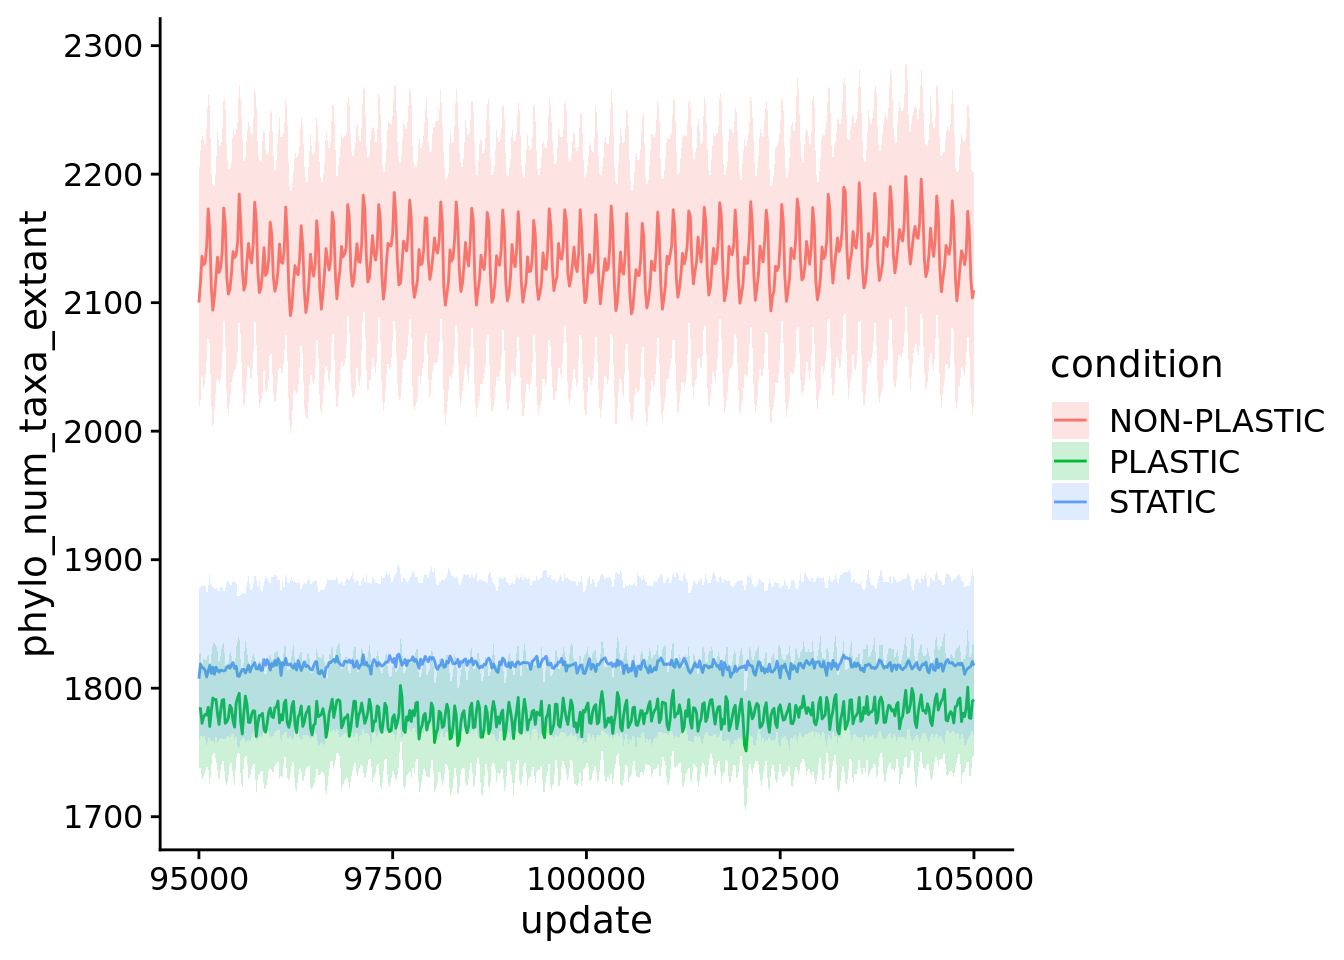
\includegraphics{supplemental-material_files/figure-latex/unnamed-chunk-27-1.pdf}

\begin{Shaded}
\begin{Highlighting}[]
\KeywordTok{paste0}\NormalTok{(}
  \StringTok{"PLASTIC: "}\NormalTok{,}
  \KeywordTok{median}\NormalTok{(}\KeywordTok{filter}\NormalTok{(summary_data, condition}\OperatorTok{==}\StringTok{"PLASTIC"}\NormalTok{)}\OperatorTok{$}\NormalTok{dominant_lineage_total_mut_cnt)}
\NormalTok{)}
\end{Highlighting}
\end{Shaded}

\begin{verbatim}
## [1] "PLASTIC: 998.5"
\end{verbatim}

\begin{Shaded}
\begin{Highlighting}[]
\KeywordTok{paste0}\NormalTok{(}
  \StringTok{"STATIC: "}\NormalTok{,}
  \KeywordTok{median}\NormalTok{(}\KeywordTok{filter}\NormalTok{(summary_data, condition}\OperatorTok{==}\StringTok{"STATIC"}\NormalTok{)}\OperatorTok{$}\NormalTok{dominant_lineage_total_mut_cnt)}
\NormalTok{)}
\end{Highlighting}
\end{Shaded}

\begin{verbatim}
## [1] "STATIC: 1100"
\end{verbatim}

\begin{Shaded}
\begin{Highlighting}[]
\KeywordTok{paste0}\NormalTok{(}
  \StringTok{"NON-PLASTIC: "}\NormalTok{,}
  \KeywordTok{median}\NormalTok{(}\KeywordTok{filter}\NormalTok{(summary_data, condition}\OperatorTok{==}\StringTok{"NON-PLASTIC"}\NormalTok{)}\OperatorTok{$}\NormalTok{dominant_lineage_total_mut_cnt)}
\NormalTok{)}
\end{Highlighting}
\end{Shaded}

\begin{verbatim}
## [1] "NON-PLASTIC: 4657.5"
\end{verbatim}

\begin{Shaded}
\begin{Highlighting}[]
\KeywordTok{kruskal.test}\NormalTok{(}
  \DataTypeTok{formula=}\NormalTok{dominant_lineage_total_mut_cnt}\OperatorTok{~}\NormalTok{condition,}
  \DataTypeTok{data=}\NormalTok{summary_data}
\NormalTok{)}
\end{Highlighting}
\end{Shaded}

\begin{verbatim}
## 
##  Kruskal-Wallis rank sum test
## 
## data:  dominant_lineage_total_mut_cnt by condition
## Kruskal-Wallis chi-squared = 179.33, df = 2, p-value < 2.2e-16
\end{verbatim}

\begin{Shaded}
\begin{Highlighting}[]
\KeywordTok{pairwise.wilcox.test}\NormalTok{(}
  \DataTypeTok{x=}\NormalTok{summary_data}\OperatorTok{$}\NormalTok{dominant_lineage_total_mut_cnt,}
  \DataTypeTok{g=}\NormalTok{summary_data}\OperatorTok{$}\NormalTok{condition,}
  \DataTypeTok{p.adjust.method=}\StringTok{"bonferroni"}\NormalTok{,}
\NormalTok{)}
\end{Highlighting}
\end{Shaded}

\begin{verbatim}
## 
##  Pairwise comparisons using Wilcoxon rank sum test with continuity correction 
## 
## data:  summary_data$dominant_lineage_total_mut_cnt and summary_data$condition 
## 
##         NON-PLASTIC PLASTIC
## PLASTIC <2e-16      -      
## STATIC  <2e-16      0.0019 
## 
## P value adjustment method: bonferroni
\end{verbatim}

\hypertarget{mutation-accumulation-normalized-by-generations-elapsed}{%
\subsection{Mutation accumulation normalized by generations elapsed}\label{mutation-accumulation-normalized-by-generations-elapsed}}

\begin{Shaded}
\begin{Highlighting}[]
\NormalTok{summary_data}\OperatorTok{$}\NormalTok{mutations_per_generation <-}\StringTok{ }\NormalTok{summary_data}\OperatorTok{$}\NormalTok{dominant_lineage_total_mut_cnt }\OperatorTok{/}\StringTok{ }\NormalTok{summary_data}\OperatorTok{$}\NormalTok{dominant_generation_born}

\KeywordTok{ggplot}\NormalTok{(summary_data, }\KeywordTok{aes}\NormalTok{(}\DataTypeTok{x=}\NormalTok{condition, }\DataTypeTok{y=}\NormalTok{mutations_per_generation, }\DataTypeTok{fill=}\NormalTok{condition)) }\OperatorTok{+}
\StringTok{  }\KeywordTok{geom_flat_violin}\NormalTok{(}
    \DataTypeTok{position =} \KeywordTok{position_nudge}\NormalTok{(}\DataTypeTok{x =} \FloatTok{.2}\NormalTok{, }\DataTypeTok{y =} \DecValTok{0}\NormalTok{),}
    \DataTypeTok{alpha =} \FloatTok{.8}
\NormalTok{  ) }\OperatorTok{+}
\StringTok{  }\KeywordTok{geom_point}\NormalTok{(}
    \DataTypeTok{mapping=}\KeywordTok{aes}\NormalTok{(}\DataTypeTok{color=}\NormalTok{condition),}
    \DataTypeTok{position =} \KeywordTok{position_jitter}\NormalTok{(}\DataTypeTok{width =} \FloatTok{.15}\NormalTok{),}
    \DataTypeTok{size =} \FloatTok{.5}\NormalTok{,}
    \DataTypeTok{alpha =} \FloatTok{0.8}
\NormalTok{  ) }\OperatorTok{+}
\StringTok{  }\KeywordTok{geom_boxplot}\NormalTok{(}
    \DataTypeTok{width =} \FloatTok{.1}\NormalTok{,}
    \DataTypeTok{outlier.shape =} \OtherTok{NA}\NormalTok{,}
    \DataTypeTok{alpha =} \FloatTok{0.5}
\NormalTok{  ) }\OperatorTok{+}
\StringTok{  }\KeywordTok{scale_x_discrete}\NormalTok{(}
    \DataTypeTok{name=}\StringTok{"Condition"}\NormalTok{,}
    \DataTypeTok{limits=}\NormalTok{condition_order}
\NormalTok{  ) }\OperatorTok{+}
\StringTok{  }\KeywordTok{ylab}\NormalTok{(}\StringTok{"Mutation accumulation / generation"}\NormalTok{) }\OperatorTok{+}
\StringTok{  }\KeywordTok{theme}\NormalTok{(}
    \DataTypeTok{legend.position=}\StringTok{"none"}
\NormalTok{  )}
\end{Highlighting}
\end{Shaded}

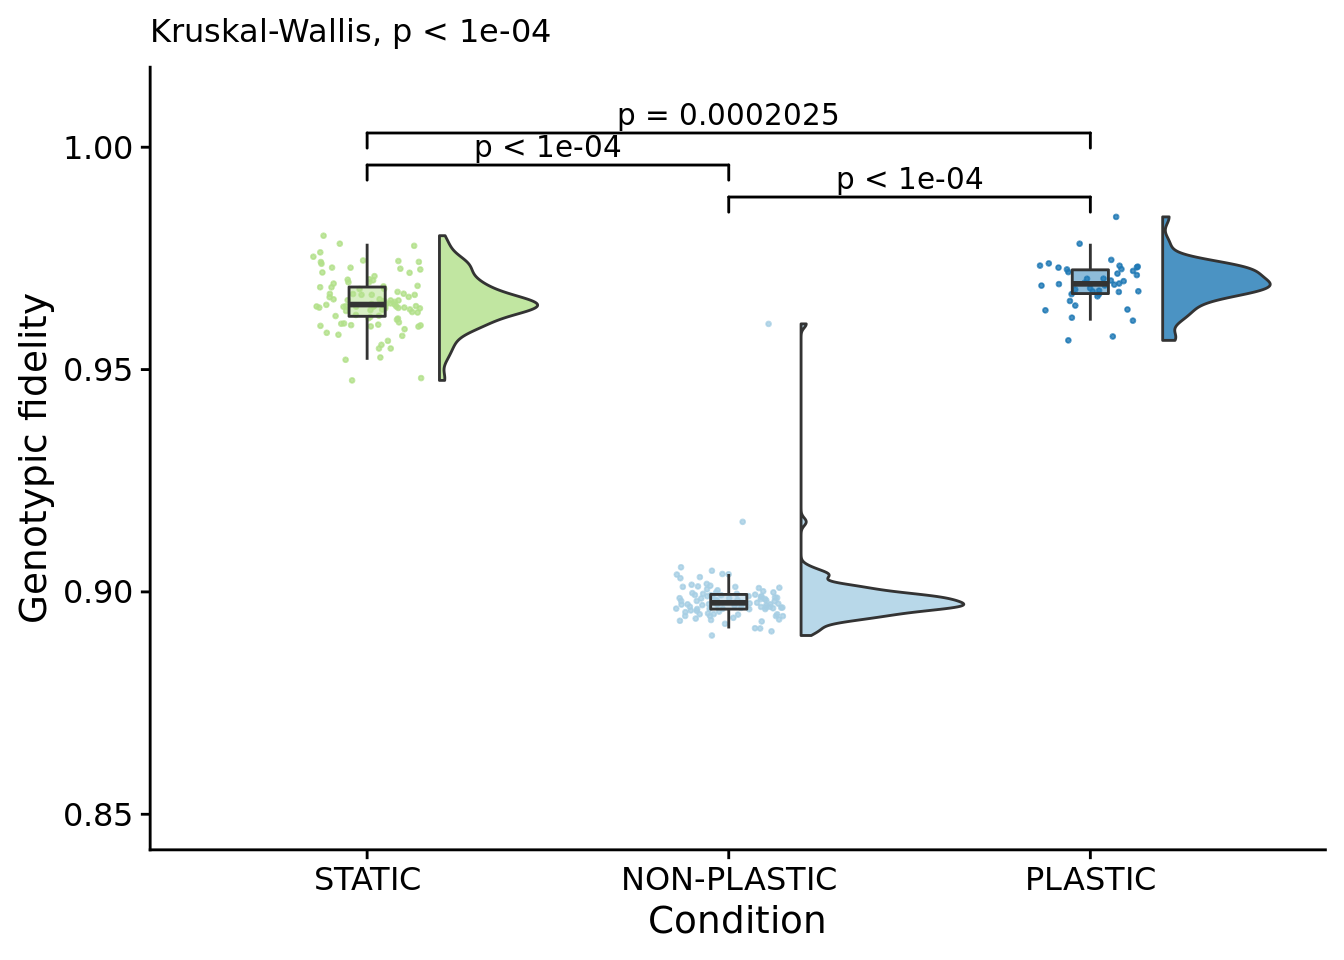
\includegraphics{supplemental-material_files/figure-latex/unnamed-chunk-29-1.pdf}

\begin{Shaded}
\begin{Highlighting}[]
\KeywordTok{paste0}\NormalTok{(}
  \StringTok{"PLASTIC: "}\NormalTok{,}
  \KeywordTok{median}\NormalTok{(}\KeywordTok{filter}\NormalTok{(summary_data, condition}\OperatorTok{==}\StringTok{"PLASTIC"}\NormalTok{)}\OperatorTok{$}\NormalTok{mutations_per_generation)}
\NormalTok{)}
\end{Highlighting}
\end{Shaded}

\begin{verbatim}
## [1] "PLASTIC: 0.0319267181456982"
\end{verbatim}

\begin{Shaded}
\begin{Highlighting}[]
\KeywordTok{paste0}\NormalTok{(}
  \StringTok{"STATIC: "}\NormalTok{,}
  \KeywordTok{median}\NormalTok{(}\KeywordTok{filter}\NormalTok{(summary_data, condition}\OperatorTok{==}\StringTok{"STATIC"}\NormalTok{)}\OperatorTok{$}\NormalTok{mutations_per_generation)}
\NormalTok{)}
\end{Highlighting}
\end{Shaded}

\begin{verbatim}
## [1] "STATIC: 0.0368157192941933"
\end{verbatim}

\begin{Shaded}
\begin{Highlighting}[]
\KeywordTok{paste0}\NormalTok{(}
  \StringTok{"NON-PLASTIC: "}\NormalTok{,}
  \KeywordTok{median}\NormalTok{(}\KeywordTok{filter}\NormalTok{(summary_data, condition}\OperatorTok{==}\StringTok{"NON-PLASTIC"}\NormalTok{)}\OperatorTok{$}\NormalTok{mutations_per_generation)}
\NormalTok{)}
\end{Highlighting}
\end{Shaded}

\begin{verbatim}
## [1] "NON-PLASTIC: 0.112804526786948"
\end{verbatim}

\begin{Shaded}
\begin{Highlighting}[]
\KeywordTok{kruskal.test}\NormalTok{(}
  \DataTypeTok{formula=}\NormalTok{mutations_per_generation}\OperatorTok{~}\NormalTok{condition,}
  \DataTypeTok{data=}\NormalTok{summary_data}
\NormalTok{)}
\end{Highlighting}
\end{Shaded}

\begin{verbatim}
## 
##  Kruskal-Wallis rank sum test
## 
## data:  mutations_per_generation by condition
## Kruskal-Wallis chi-squared = 180.11, df = 2, p-value < 2.2e-16
\end{verbatim}

\begin{Shaded}
\begin{Highlighting}[]
\KeywordTok{pairwise.wilcox.test}\NormalTok{(}
  \DataTypeTok{x=}\NormalTok{summary_data}\OperatorTok{$}\NormalTok{mutations_per_generation,}
  \DataTypeTok{g=}\NormalTok{summary_data}\OperatorTok{$}\NormalTok{condition,}
  \DataTypeTok{p.adjust.method=}\StringTok{"bonferroni"}\NormalTok{,}
\NormalTok{)}
\end{Highlighting}
\end{Shaded}

\begin{verbatim}
## 
##  Pairwise comparisons using Wilcoxon rank sum test with continuity correction 
## 
## data:  summary_data$mutations_per_generation and summary_data$condition 
## 
##         NON-PLASTIC PLASTIC
## PLASTIC <2e-16      -      
## STATIC  <2e-16      2e-04  
## 
## P value adjustment method: bonferroni
\end{verbatim}

\hypertarget{mutation-accumulation-normalized-by-lineage-length}{%
\subsection{Mutation accumulation normalized by lineage length}\label{mutation-accumulation-normalized-by-lineage-length}}

\begin{Shaded}
\begin{Highlighting}[]
\NormalTok{summary_data}\OperatorTok{$}\NormalTok{mutations_per_lineage_step <-}\StringTok{ }\NormalTok{summary_data}\OperatorTok{$}\NormalTok{dominant_lineage_total_mut_cnt }\OperatorTok{/}\StringTok{ }\NormalTok{summary_data}\OperatorTok{$}\NormalTok{dominant_lineage_length_genotypes}
\KeywordTok{ggplot}\NormalTok{(summary_data, }\KeywordTok{aes}\NormalTok{(}\DataTypeTok{x=}\NormalTok{condition, }\DataTypeTok{y=}\NormalTok{mutations_per_lineage_step, }\DataTypeTok{fill=}\NormalTok{condition)) }\OperatorTok{+}
\StringTok{  }\KeywordTok{geom_flat_violin}\NormalTok{(}
    \DataTypeTok{position =} \KeywordTok{position_nudge}\NormalTok{(}\DataTypeTok{x =} \FloatTok{.2}\NormalTok{, }\DataTypeTok{y =} \DecValTok{0}\NormalTok{),}
    \DataTypeTok{alpha =} \FloatTok{.8}
\NormalTok{  ) }\OperatorTok{+}
\StringTok{  }\KeywordTok{geom_point}\NormalTok{(}
    \DataTypeTok{mapping=}\KeywordTok{aes}\NormalTok{(}\DataTypeTok{color=}\NormalTok{condition),}
    \DataTypeTok{position =} \KeywordTok{position_jitter}\NormalTok{(}\DataTypeTok{width =} \FloatTok{.15}\NormalTok{),}
    \DataTypeTok{size =} \FloatTok{.5}\NormalTok{,}
    \DataTypeTok{alpha =} \FloatTok{0.8}
\NormalTok{  ) }\OperatorTok{+}
\StringTok{  }\KeywordTok{geom_boxplot}\NormalTok{(}
    \DataTypeTok{width =} \FloatTok{.1}\NormalTok{,}
    \DataTypeTok{outlier.shape =} \OtherTok{NA}\NormalTok{,}
    \DataTypeTok{alpha =} \FloatTok{0.5}
\NormalTok{  ) }\OperatorTok{+}
\StringTok{  }\KeywordTok{scale_x_discrete}\NormalTok{(}
    \DataTypeTok{name=}\StringTok{"Condition"}\NormalTok{,}
    \DataTypeTok{limits=}\NormalTok{condition_order}
\NormalTok{  ) }\OperatorTok{+}
\StringTok{  }\KeywordTok{ylab}\NormalTok{(}\StringTok{"Mutation accumulation / lineage length"}\NormalTok{) }\OperatorTok{+}
\StringTok{  }\KeywordTok{theme}\NormalTok{(}
    \DataTypeTok{legend.position=}\StringTok{"none"}
\NormalTok{  )}
\end{Highlighting}
\end{Shaded}

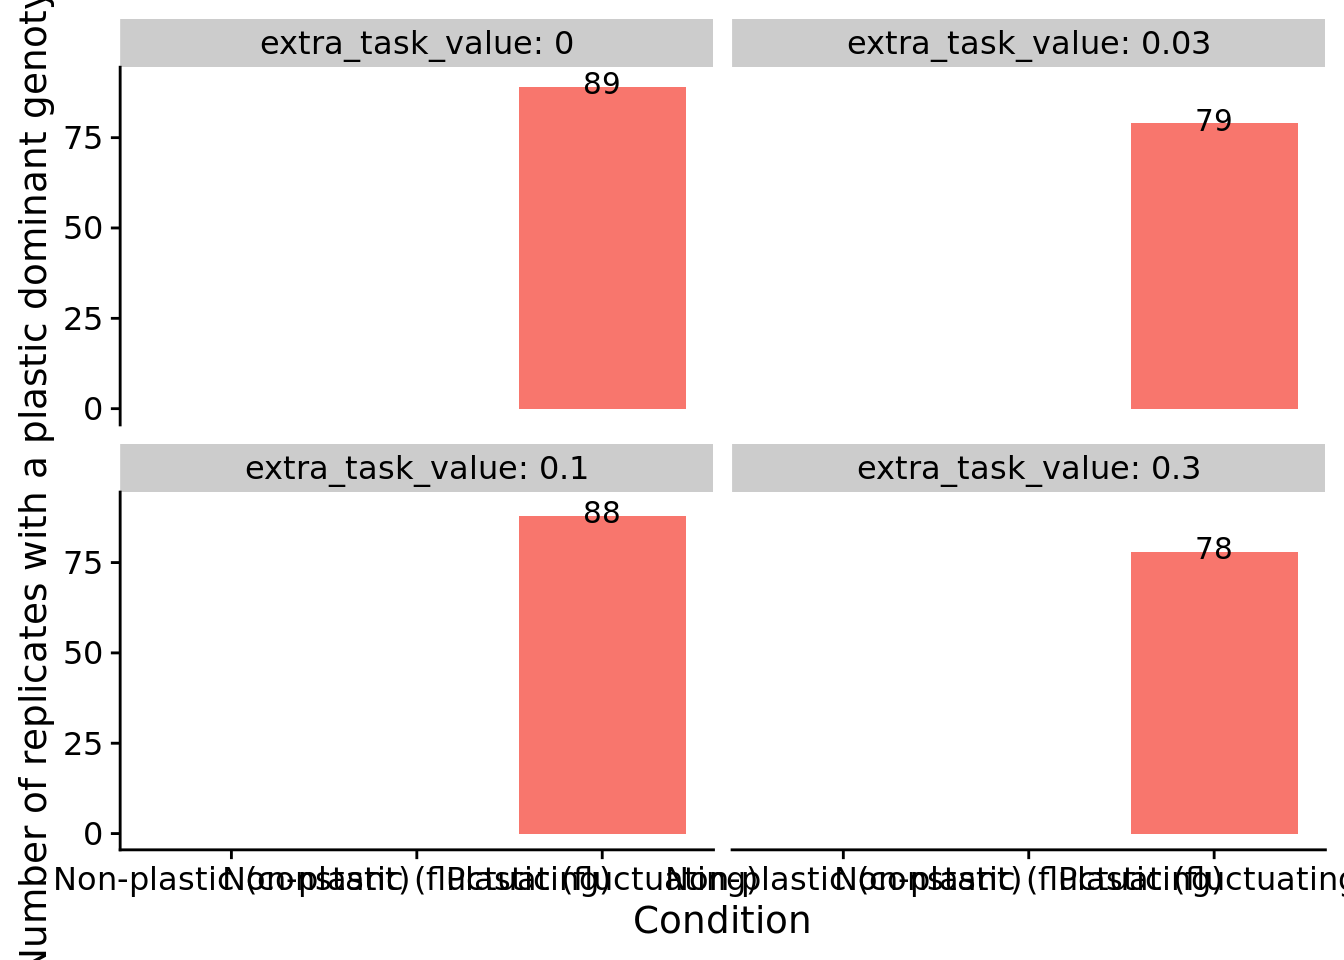
\includegraphics{supplemental-material_files/figure-latex/unnamed-chunk-31-1.pdf}

\begin{Shaded}
\begin{Highlighting}[]
\KeywordTok{paste0}\NormalTok{(}
  \StringTok{"PLASTIC: "}\NormalTok{,}
  \KeywordTok{median}\NormalTok{(}\KeywordTok{filter}\NormalTok{(summary_data, condition}\OperatorTok{==}\StringTok{"PLASTIC"}\NormalTok{)}\OperatorTok{$}\NormalTok{mutations_per_lineage_step)}
\NormalTok{)}
\end{Highlighting}
\end{Shaded}

\begin{verbatim}
## [1] "PLASTIC: 1.0328599144651"
\end{verbatim}

\begin{Shaded}
\begin{Highlighting}[]
\KeywordTok{paste0}\NormalTok{(}
  \StringTok{"STATIC: "}\NormalTok{,}
  \KeywordTok{median}\NormalTok{(}\KeywordTok{filter}\NormalTok{(summary_data, condition}\OperatorTok{==}\StringTok{"STATIC"}\NormalTok{)}\OperatorTok{$}\NormalTok{mutations_per_lineage_step)}
\NormalTok{)}
\end{Highlighting}
\end{Shaded}

\begin{verbatim}
## [1] "STATIC: 1.03794597464116"
\end{verbatim}

\begin{Shaded}
\begin{Highlighting}[]
\KeywordTok{paste0}\NormalTok{(}
  \StringTok{"NON-PLASTIC: "}\NormalTok{,}
  \KeywordTok{median}\NormalTok{(}\KeywordTok{filter}\NormalTok{(summary_data, condition}\OperatorTok{==}\StringTok{"NON-PLASTIC"}\NormalTok{)}\OperatorTok{$}\NormalTok{mutations_per_lineage_step)}
\NormalTok{)}
\end{Highlighting}
\end{Shaded}

\begin{verbatim}
## [1] "NON-PLASTIC: 1.10048311715591"
\end{verbatim}

\begin{Shaded}
\begin{Highlighting}[]
\KeywordTok{kruskal.test}\NormalTok{(}
  \DataTypeTok{formula=}\NormalTok{mutations_per_lineage_step}\OperatorTok{~}\NormalTok{condition,}
  \DataTypeTok{data=}\NormalTok{summary_data}
\NormalTok{)}
\end{Highlighting}
\end{Shaded}

\begin{verbatim}
## 
##  Kruskal-Wallis rank sum test
## 
## data:  mutations_per_lineage_step by condition
## Kruskal-Wallis chi-squared = 178.92, df = 2, p-value < 2.2e-16
\end{verbatim}

\begin{Shaded}
\begin{Highlighting}[]
\KeywordTok{pairwise.wilcox.test}\NormalTok{(}
  \DataTypeTok{x=}\NormalTok{summary_data}\OperatorTok{$}\NormalTok{mutations_per_lineage_step,}
  \DataTypeTok{g=}\NormalTok{summary_data}\OperatorTok{$}\NormalTok{condition,}
  \DataTypeTok{p.adjust.method=}\StringTok{"bonferroni"}\NormalTok{,}
\NormalTok{)}
\end{Highlighting}
\end{Shaded}

\begin{verbatim}
## 
##  Pairwise comparisons using Wilcoxon rank sum test with continuity correction 
## 
## data:  summary_data$mutations_per_lineage_step and summary_data$condition 
## 
##         NON-PLASTIC PLASTIC
## PLASTIC <2e-16      -      
## STATIC  <2e-16      0.0034 
## 
## P value adjustment method: bonferroni
\end{verbatim}

\hypertarget{genotypic-fidelity}{%
\subsection{Genotypic fidelity}\label{genotypic-fidelity}}

The frequency that an offspring's genotype is the same as a parent's genotype.

\begin{Shaded}
\begin{Highlighting}[]
\NormalTok{summary_data}\OperatorTok{$}\NormalTok{dominant_lineage_genotypic_fidelity <-}\StringTok{ }\NormalTok{(summary_data}\OperatorTok{$}\NormalTok{dominant_generation_born }\OperatorTok{-}\StringTok{ }\NormalTok{summary_data}\OperatorTok{$}\NormalTok{dominant_lineage_num_mut_steps) }\OperatorTok{/}\StringTok{ }\NormalTok{summary_data}\OperatorTok{$}\NormalTok{dominant_generation_born}

\KeywordTok{ggplot}\NormalTok{(summary_data, }\KeywordTok{aes}\NormalTok{(}\DataTypeTok{x=}\NormalTok{condition, }\DataTypeTok{y=}\NormalTok{dominant_lineage_genotypic_fidelity, }\DataTypeTok{fill=}\NormalTok{condition)) }\OperatorTok{+}
\StringTok{  }\KeywordTok{geom_flat_violin}\NormalTok{(}
    \DataTypeTok{position =} \KeywordTok{position_nudge}\NormalTok{(}\DataTypeTok{x =} \FloatTok{.2}\NormalTok{, }\DataTypeTok{y =} \DecValTok{0}\NormalTok{),}
    \DataTypeTok{alpha =} \FloatTok{.8}
\NormalTok{  ) }\OperatorTok{+}
\StringTok{  }\KeywordTok{geom_point}\NormalTok{(}
    \DataTypeTok{mapping=}\KeywordTok{aes}\NormalTok{(}\DataTypeTok{color=}\NormalTok{condition),}
    \DataTypeTok{position =} \KeywordTok{position_jitter}\NormalTok{(}\DataTypeTok{width =} \FloatTok{.15}\NormalTok{),}
    \DataTypeTok{size =} \FloatTok{.5}\NormalTok{,}
    \DataTypeTok{alpha =} \FloatTok{0.8}
\NormalTok{  ) }\OperatorTok{+}
\StringTok{  }\KeywordTok{geom_boxplot}\NormalTok{(}
    \DataTypeTok{width =} \FloatTok{.1}\NormalTok{,}
    \DataTypeTok{outlier.shape =} \OtherTok{NA}\NormalTok{,}
    \DataTypeTok{alpha =} \FloatTok{0.5}
\NormalTok{  ) }\OperatorTok{+}
\StringTok{  }\KeywordTok{scale_x_discrete}\NormalTok{(}
    \DataTypeTok{name=}\StringTok{"Condition"}\NormalTok{,}
    \DataTypeTok{limits=}\NormalTok{condition_order}
\NormalTok{  ) }\OperatorTok{+}
\StringTok{  }\KeywordTok{theme}\NormalTok{(}
    \DataTypeTok{legend.position=}\StringTok{"none"}
\NormalTok{  )}
\end{Highlighting}
\end{Shaded}

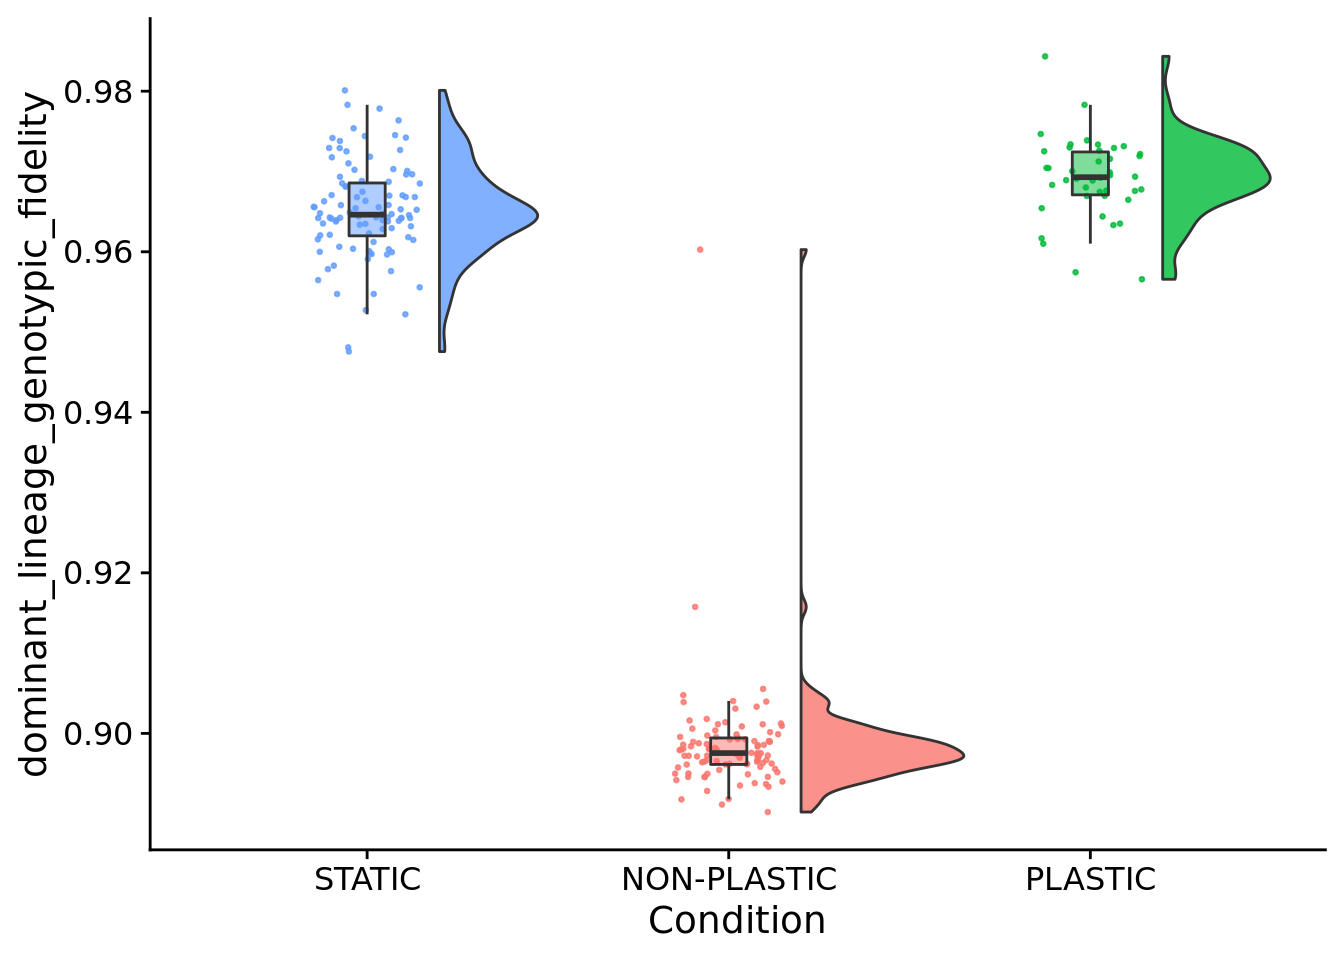
\includegraphics{supplemental-material_files/figure-latex/unnamed-chunk-33-1.pdf}

\begin{Shaded}
\begin{Highlighting}[]
\KeywordTok{paste0}\NormalTok{(}
  \StringTok{"PLASTIC: "}\NormalTok{,}
  \KeywordTok{median}\NormalTok{(}\KeywordTok{filter}\NormalTok{(summary_data, condition}\OperatorTok{==}\StringTok{"PLASTIC"}\NormalTok{)}\OperatorTok{$}\NormalTok{dominant_lineage_genotypic_fidelity)}
\NormalTok{)}
\end{Highlighting}
\end{Shaded}

\begin{verbatim}
## [1] "PLASTIC: 0.969286906891951"
\end{verbatim}

\begin{Shaded}
\begin{Highlighting}[]
\KeywordTok{paste0}\NormalTok{(}
  \StringTok{"STATIC: "}\NormalTok{,}
  \KeywordTok{median}\NormalTok{(}\KeywordTok{filter}\NormalTok{(summary_data, condition}\OperatorTok{==}\StringTok{"STATIC"}\NormalTok{)}\OperatorTok{$}\NormalTok{dominant_lineage_genotypic_fidelity)}
\NormalTok{)}
\end{Highlighting}
\end{Shaded}

\begin{verbatim}
## [1] "STATIC: 0.964620594632577"
\end{verbatim}

\begin{Shaded}
\begin{Highlighting}[]
\KeywordTok{paste0}\NormalTok{(}
  \StringTok{"NON-PLASTIC: "}\NormalTok{,}
  \KeywordTok{median}\NormalTok{(}\KeywordTok{filter}\NormalTok{(summary_data, condition}\OperatorTok{==}\StringTok{"NON-PLASTIC"}\NormalTok{)}\OperatorTok{$}\NormalTok{dominant_lineage_genotypic_fidelity)}
\NormalTok{)}
\end{Highlighting}
\end{Shaded}

\begin{verbatim}
## [1] "NON-PLASTIC: 0.89754902563783"
\end{verbatim}

\begin{Shaded}
\begin{Highlighting}[]
\KeywordTok{kruskal.test}\NormalTok{(}
  \DataTypeTok{formula=}\NormalTok{dominant_lineage_genotypic_fidelity}\OperatorTok{~}\NormalTok{condition,}
  \DataTypeTok{data=}\NormalTok{summary_data}
\NormalTok{)}
\end{Highlighting}
\end{Shaded}

\begin{verbatim}
## 
##  Kruskal-Wallis rank sum test
## 
## data:  dominant_lineage_genotypic_fidelity by condition
## Kruskal-Wallis chi-squared = 179.86, df = 2, p-value < 2.2e-16
\end{verbatim}

\begin{Shaded}
\begin{Highlighting}[]
\KeywordTok{pairwise.wilcox.test}\NormalTok{(}
  \DataTypeTok{x=}\NormalTok{summary_data}\OperatorTok{$}\NormalTok{dominant_lineage_genotypic_fidelity,}
  \DataTypeTok{g=}\NormalTok{summary_data}\OperatorTok{$}\NormalTok{condition,}
  \DataTypeTok{p.adjust.method=}\StringTok{"bonferroni"}\NormalTok{,}
\NormalTok{)}
\end{Highlighting}
\end{Shaded}

\begin{verbatim}
## 
##  Pairwise comparisons using Wilcoxon rank sum test with continuity correction 
## 
## data:  summary_data$dominant_lineage_genotypic_fidelity and summary_data$condition 
## 
##         NON-PLASTIC PLASTIC
## PLASTIC <2e-16      -      
## STATIC  <2e-16      2e-04  
## 
## P value adjustment method: bonferroni
\end{verbatim}

\hypertarget{characterizing-variation-along-lineages}{%
\subsection{Characterizing variation along lineages}\label{characterizing-variation-along-lineages}}

\hypertarget{how-many-mutation-steps-along-the-lineage-result-in-phenotypic-changes}{%
\subsubsection{How many mutation-steps along the lineage result in phenotypic changes?}\label{how-many-mutation-steps-along-the-lineage-result-in-phenotypic-changes}}

\begin{Shaded}
\begin{Highlighting}[]
\NormalTok{summary_data}\OperatorTok{$}\NormalTok{frac_phenotype_changing_mut_steps <-}\StringTok{ }\NormalTok{summary_data}\OperatorTok{$}\NormalTok{dominant_lineage_num_mut_steps_that_change_aggregate_phenotype }\OperatorTok{/}\StringTok{ }\NormalTok{summary_data}\OperatorTok{$}\NormalTok{dominant_lineage_num_mut_steps}

\KeywordTok{ggplot}\NormalTok{(}\KeywordTok{filter}\NormalTok{(summary_data, dominant_lineage_num_mut_steps }\OperatorTok{>}\StringTok{ }\DecValTok{0}\NormalTok{), }\KeywordTok{aes}\NormalTok{(}\DataTypeTok{x=}\NormalTok{frac_phenotype_changing_mut_steps)) }\OperatorTok{+}
\StringTok{  }\KeywordTok{geom_density}\NormalTok{() }\OperatorTok{+}
\StringTok{  }\KeywordTok{facet_wrap}\NormalTok{(}
    \OperatorTok{~}\NormalTok{condition,}
    \DataTypeTok{nrow=}\DecValTok{3}\NormalTok{,}
    \DataTypeTok{labeller=}\NormalTok{label_both}

\NormalTok{  ) }\OperatorTok{+}
\StringTok{  }\KeywordTok{xlim}\NormalTok{(}\DecValTok{0}\NormalTok{, }\FloatTok{1.0}\NormalTok{) }\OperatorTok{+}
\StringTok{  }\KeywordTok{theme}\NormalTok{(}
    \DataTypeTok{legend.position=}\StringTok{"none"}
\NormalTok{  )}
\end{Highlighting}
\end{Shaded}

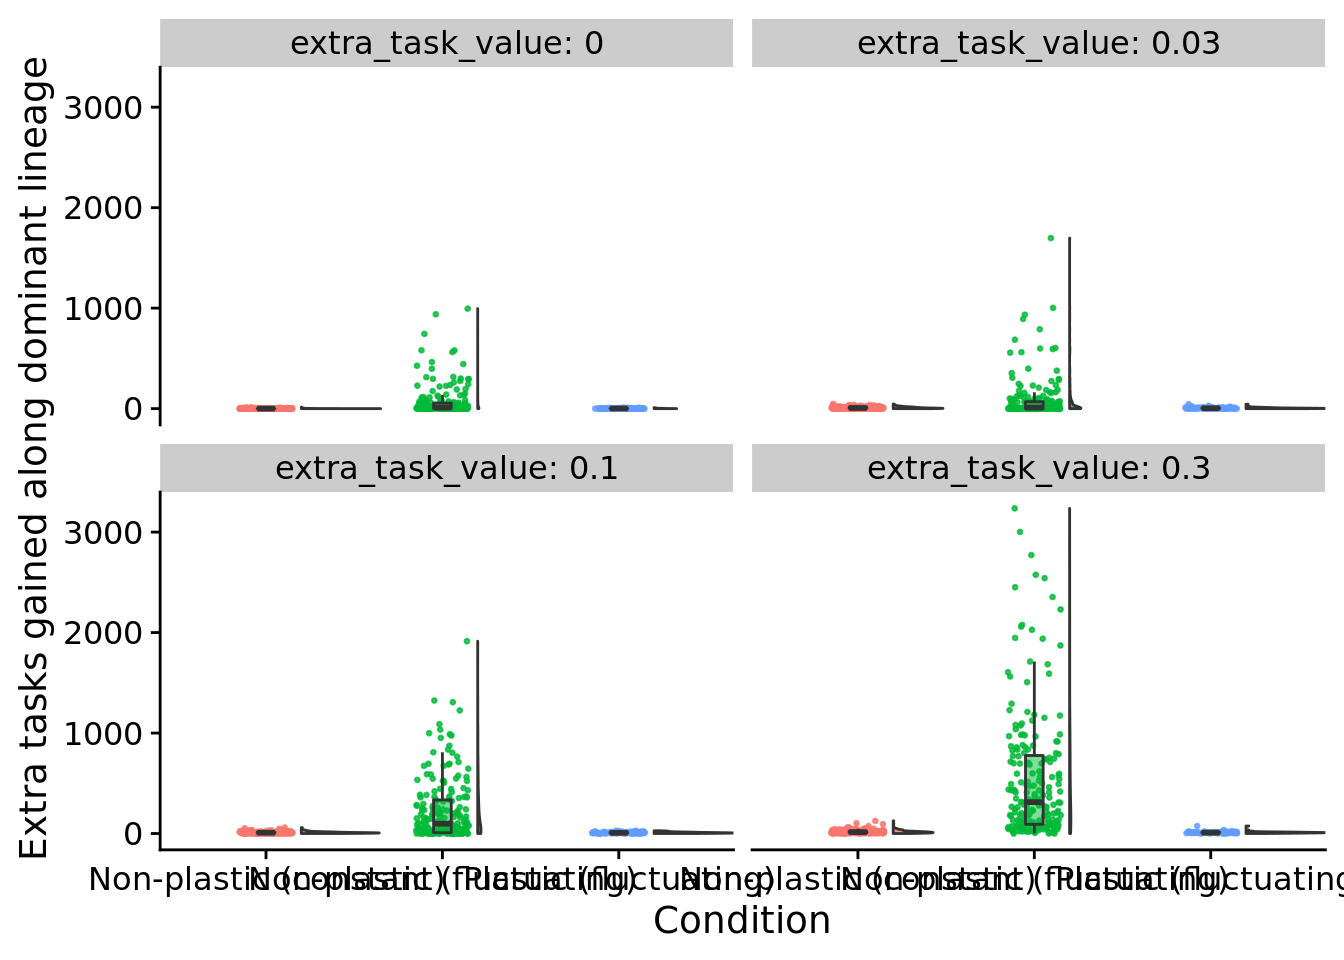
\includegraphics{supplemental-material_files/figure-latex/unnamed-chunk-35-1.pdf}

\begin{Shaded}
\begin{Highlighting}[]
\KeywordTok{ggplot}\NormalTok{(summary_data, }\KeywordTok{aes}\NormalTok{(}\DataTypeTok{x=}\NormalTok{condition, }\DataTypeTok{y=}\NormalTok{frac_phenotype_changing_mut_steps, }\DataTypeTok{fill=}\NormalTok{condition)) }\OperatorTok{+}
\StringTok{  }\KeywordTok{geom_flat_violin}\NormalTok{(}
    \DataTypeTok{position =} \KeywordTok{position_nudge}\NormalTok{(}\DataTypeTok{x =} \FloatTok{.2}\NormalTok{, }\DataTypeTok{y =} \DecValTok{0}\NormalTok{),}
    \DataTypeTok{alpha =} \FloatTok{.8}
\NormalTok{  ) }\OperatorTok{+}
\StringTok{  }\KeywordTok{geom_point}\NormalTok{(}
    \DataTypeTok{mapping=}\KeywordTok{aes}\NormalTok{(}\DataTypeTok{color=}\NormalTok{condition),}
    \DataTypeTok{position =} \KeywordTok{position_jitter}\NormalTok{(}\DataTypeTok{width =} \FloatTok{.15}\NormalTok{),}
    \DataTypeTok{size =} \FloatTok{.5}\NormalTok{,}
    \DataTypeTok{alpha =} \FloatTok{0.8}
\NormalTok{  ) }\OperatorTok{+}
\StringTok{  }\KeywordTok{geom_boxplot}\NormalTok{(}
    \DataTypeTok{width =} \FloatTok{.1}\NormalTok{,}
    \DataTypeTok{outlier.shape =} \OtherTok{NA}\NormalTok{,}
    \DataTypeTok{alpha =} \FloatTok{0.5}
\NormalTok{  ) }\OperatorTok{+}
\StringTok{  }\KeywordTok{scale_x_discrete}\NormalTok{(}
    \DataTypeTok{name=}\StringTok{"Condition"}\NormalTok{,}
    \DataTypeTok{limits=}\NormalTok{condition_order}
\NormalTok{  ) }\OperatorTok{+}
\StringTok{  }\KeywordTok{theme}\NormalTok{(}
    \DataTypeTok{legend.position=}\StringTok{"none"}
\NormalTok{  )}
\end{Highlighting}
\end{Shaded}

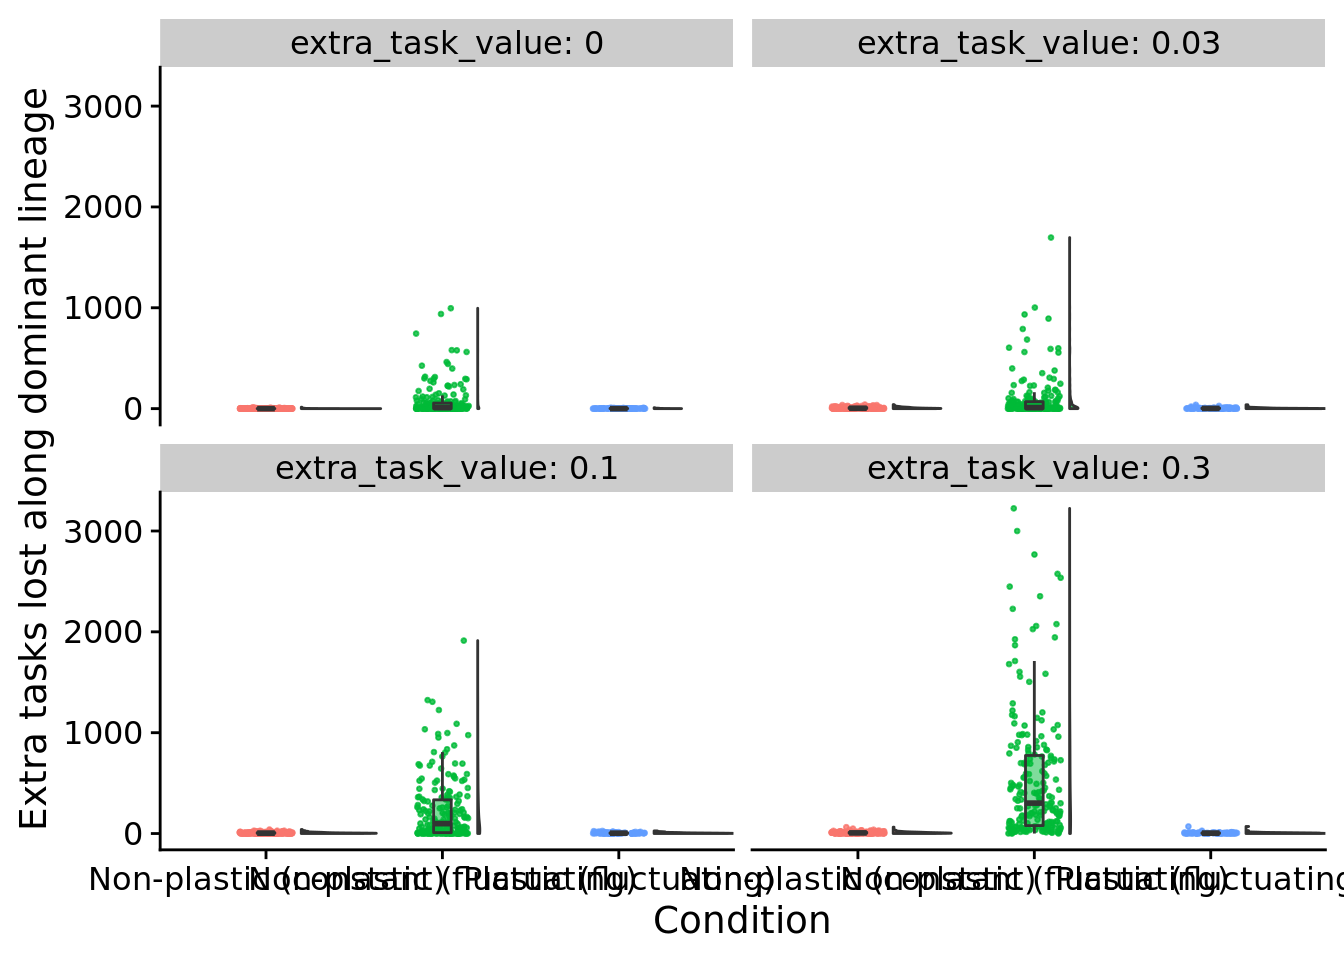
\includegraphics{supplemental-material_files/figure-latex/unnamed-chunk-36-1.pdf}

\begin{Shaded}
\begin{Highlighting}[]
\KeywordTok{paste0}\NormalTok{(}
  \StringTok{"PLASTIC: "}\NormalTok{,}
  \KeywordTok{median}\NormalTok{(}\KeywordTok{filter}\NormalTok{(summary_data, condition}\OperatorTok{==}\StringTok{"PLASTIC"}\NormalTok{)}\OperatorTok{$}\NormalTok{frac_phenotype_changing_mut_steps)}
\NormalTok{)}
\end{Highlighting}
\end{Shaded}

\begin{verbatim}
## [1] "PLASTIC: 0.00224941742616098"
\end{verbatim}

\begin{Shaded}
\begin{Highlighting}[]
\KeywordTok{paste0}\NormalTok{(}
  \StringTok{"STATIC: "}\NormalTok{,}
  \KeywordTok{median}\NormalTok{(}\KeywordTok{filter}\NormalTok{(summary_data, condition}\OperatorTok{==}\StringTok{"STATIC"}\NormalTok{)}\OperatorTok{$}\NormalTok{frac_phenotype_changing_mut_steps)}
\NormalTok{)}
\end{Highlighting}
\end{Shaded}

\begin{verbatim}
## [1] "STATIC: 0"
\end{verbatim}

\begin{Shaded}
\begin{Highlighting}[]
\KeywordTok{paste0}\NormalTok{(}
  \StringTok{"NON-PLASTIC: "}\NormalTok{,}
  \KeywordTok{median}\NormalTok{(}\KeywordTok{filter}\NormalTok{(summary_data, condition}\OperatorTok{==}\StringTok{"NON-PLASTIC"}\NormalTok{)}\OperatorTok{$}\NormalTok{frac_phenotype_changing_mut_steps)}
\NormalTok{)}
\end{Highlighting}
\end{Shaded}

\begin{verbatim}
## [1] "NON-PLASTIC: 0.437583018324547"
\end{verbatim}

\begin{Shaded}
\begin{Highlighting}[]
\KeywordTok{kruskal.test}\NormalTok{(}
  \DataTypeTok{formula=}\NormalTok{frac_phenotype_changing_mut_steps}\OperatorTok{~}\NormalTok{condition,}
  \DataTypeTok{data=}\NormalTok{summary_data}
\NormalTok{)}
\end{Highlighting}
\end{Shaded}

\begin{verbatim}
## 
##  Kruskal-Wallis rank sum test
## 
## data:  frac_phenotype_changing_mut_steps by condition
## Kruskal-Wallis chi-squared = 191.23, df = 2, p-value < 2.2e-16
\end{verbatim}

\begin{Shaded}
\begin{Highlighting}[]
\KeywordTok{pairwise.wilcox.test}\NormalTok{(}
  \DataTypeTok{x=}\NormalTok{summary_data}\OperatorTok{$}\NormalTok{frac_phenotype_changing_mut_steps,}
  \DataTypeTok{g=}\NormalTok{summary_data}\OperatorTok{$}\NormalTok{condition,}
  \DataTypeTok{p.adjust.method=}\StringTok{"bonferroni"}\NormalTok{,}
\NormalTok{)}
\end{Highlighting}
\end{Shaded}

\begin{verbatim}
## 
##  Pairwise comparisons using Wilcoxon rank sum test with continuity correction 
## 
## data:  summary_data$frac_phenotype_changing_mut_steps and summary_data$condition 
## 
##         NON-PLASTIC PLASTIC
## PLASTIC < 2e-16     -      
## STATIC  < 2e-16     2.3e-07
## 
## P value adjustment method: bonferroni
\end{verbatim}

\hypertarget{for-plastic-populations-what-fraction-of-phenotype-altering-mutations-affect-the-unexpressed-phenotype}{%
\subsubsection{For PLASTIC populations, what fraction of phenotype-altering mutations affect the unexpressed phenotype?}\label{for-plastic-populations-what-fraction-of-phenotype-altering-mutations-affect-the-unexpressed-phenotype}}

\begin{Shaded}
\begin{Highlighting}[]
\NormalTok{summary_data}\OperatorTok{$}\NormalTok{frac_unexpressed_mut_steps <-}\StringTok{ }\NormalTok{summary_data}\OperatorTok{$}\NormalTok{dominant_lineage_num_mut_steps_that_change_unexpressed_phenotype }\OperatorTok{/}\StringTok{ }\NormalTok{summary_data}\OperatorTok{$}\NormalTok{dominant_lineage_num_mut_steps_that_change_aggregate_phenotype}
\NormalTok{summary_data}\OperatorTok{$}\NormalTok{frac_expressed_mut_steps <-}\StringTok{ }\NormalTok{summary_data}\OperatorTok{$}\NormalTok{dominant_lineage_num_mut_steps_that_change_expressed_phenotype }\OperatorTok{/}\StringTok{ }\NormalTok{summary_data}\OperatorTok{$}\NormalTok{dominant_lineage_num_mut_steps_that_change_aggregate_phenotype}

\KeywordTok{ggplot}\NormalTok{(}\KeywordTok{filter}\NormalTok{(summary_data, condition}\OperatorTok{==}\StringTok{"PLASTIC"} \OperatorTok{&}\StringTok{ }\NormalTok{dominant_lineage_num_mut_steps_that_change_aggregate_phenotype }\OperatorTok{>}\StringTok{ }\DecValTok{0}\NormalTok{), }\KeywordTok{aes}\NormalTok{(}\DataTypeTok{x=}\NormalTok{frac_unexpressed_mut_steps)) }\OperatorTok{+}
\StringTok{  }\KeywordTok{geom_density}\NormalTok{() }\OperatorTok{+}
\StringTok{  }\KeywordTok{theme}\NormalTok{(}
    \DataTypeTok{legend.position=}\StringTok{"none"}
\NormalTok{  )}
\end{Highlighting}
\end{Shaded}

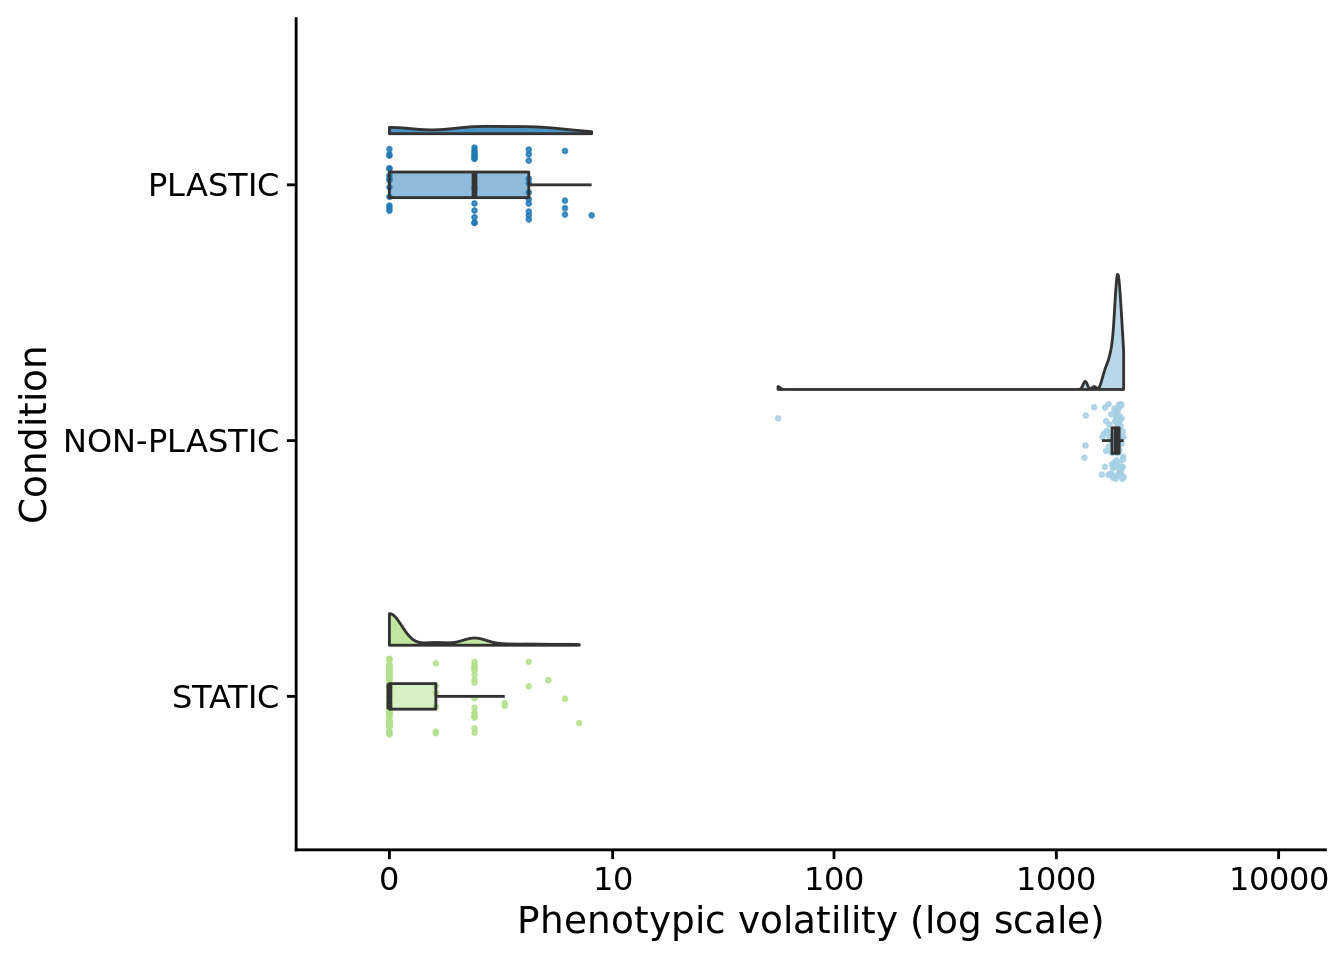
\includegraphics{supplemental-material_files/figure-latex/unnamed-chunk-39-1.pdf}

\begin{Shaded}
\begin{Highlighting}[]
\KeywordTok{print}\NormalTok{(}\KeywordTok{paste0}\NormalTok{(}\StringTok{"PLASTIC - Mean with bootstrapped 95% CI"}\NormalTok{))}
\end{Highlighting}
\end{Shaded}

\begin{verbatim}
## [1] "PLASTIC - Mean with bootstrapped 95% CI"
\end{verbatim}

\begin{Shaded}
\begin{Highlighting}[]
\NormalTok{bo <-}\StringTok{ }\KeywordTok{boot}\NormalTok{(}\KeywordTok{filter}\NormalTok{(summary_data, condition}\OperatorTok{==}\StringTok{"PLASTIC"} \OperatorTok{&}\StringTok{ }\NormalTok{dominant_lineage_num_mut_steps_that_change_aggregate_phenotype }\OperatorTok{>}\StringTok{ }\DecValTok{0}\NormalTok{)}\OperatorTok{$}\NormalTok{frac_unexpressed_mut_steps, }\DataTypeTok{statistic=}\NormalTok{samplemean, }\DataTypeTok{R=}\DecValTok{10000}\NormalTok{)}
\KeywordTok{print}\NormalTok{(bo)}
\end{Highlighting}
\end{Shaded}

\begin{verbatim}
## 
## ORDINARY NONPARAMETRIC BOOTSTRAP
## 
## 
## Call:
## boot(data = filter(summary_data, condition == "PLASTIC" & dominant_lineage_num_mut_steps_that_change_aggregate_phenotype > 
##     0)$frac_unexpressed_mut_steps, statistic = samplemean, R = 10000)
## 
## 
## Bootstrap Statistics :
##      original        bias    std. error
## t1* 0.8247126 -0.0003258621   0.0404859
\end{verbatim}

\begin{Shaded}
\begin{Highlighting}[]
\KeywordTok{print}\NormalTok{(}\KeywordTok{boot.ci}\NormalTok{(bo, }\DataTypeTok{conf=}\FloatTok{0.95}\NormalTok{, }\DataTypeTok{type=}\StringTok{"perc"}\NormalTok{))}
\end{Highlighting}
\end{Shaded}

\begin{verbatim}
## BOOTSTRAP CONFIDENCE INTERVAL CALCULATIONS
## Based on 10000 bootstrap replicates
## 
## CALL : 
## boot.ci(boot.out = bo, conf = 0.95, type = "perc")
## 
## Intervals : 
## Level     Percentile     
## 95%   ( 0.7414,  0.8994 )  
## Calculations and Intervals on Original Scale
\end{verbatim}

\begin{Shaded}
\begin{Highlighting}[]
\NormalTok{plastic_summary_data <-}\StringTok{ }\KeywordTok{filter}\NormalTok{(summary_data, condition}\OperatorTok{==}\StringTok{"PLASTIC"}\NormalTok{)}
\NormalTok{aggregate_frac_mut_steps_that_change_unexpressed_phenotype <-}\StringTok{ }\KeywordTok{sum}\NormalTok{(plastic_summary_data}\OperatorTok{$}\NormalTok{dominant_lineage_num_mut_steps_that_change_unexpressed_phenotype) }\OperatorTok{/}\StringTok{ }\KeywordTok{sum}\NormalTok{(plastic_summary_data}\OperatorTok{$}\NormalTok{dominant_lineage_num_mut_steps_that_change_aggregate_phenotype)}
\KeywordTok{sum}\NormalTok{(plastic_summary_data}\OperatorTok{$}\NormalTok{dominant_lineage_num_mut_steps_that_change_unexpressed_phenotype)}
\end{Highlighting}
\end{Shaded}

\begin{verbatim}
## [1] 83
\end{verbatim}

\begin{Shaded}
\begin{Highlighting}[]
\KeywordTok{sum}\NormalTok{(plastic_summary_data}\OperatorTok{$}\NormalTok{dominant_lineage_num_mut_steps_that_change_aggregate_phenotype)}
\end{Highlighting}
\end{Shaded}

\begin{verbatim}
## [1] 102
\end{verbatim}

\begin{Shaded}
\begin{Highlighting}[]
\NormalTok{aggregate_frac_mut_steps_that_change_unexpressed_phenotype}
\end{Highlighting}
\end{Shaded}

\begin{verbatim}
## [1] 0.8137255
\end{verbatim}

83 / 102 (0.8137255)

\hypertarget{for-plastic-populations-what-fraction-of-mutations-that-affect-the-unexpressed-phenotype-are-deleterious-versus-beneficial}{%
\subsubsection{For PLASTIC populations, what fraction of mutations that affect the unexpressed phenotype are deleterious versus beneficial?}\label{for-plastic-populations-what-fraction-of-mutations-that-affect-the-unexpressed-phenotype-are-deleterious-versus-beneficial}}

\begin{Shaded}
\begin{Highlighting}[]
\NormalTok{aggregate_frac_unexpressed_deleterious_mut_steps <-}\StringTok{ }\KeywordTok{sum}\NormalTok{(plastic_summary_data}\OperatorTok{$}\NormalTok{dominant_lineage_num_mut_steps_that_change_unexpressed_phenotype_deleterious) }\OperatorTok{/}\StringTok{ }\KeywordTok{sum}\NormalTok{(plastic_summary_data}\OperatorTok{$}\NormalTok{dominant_lineage_num_mut_steps_that_change_unexpressed_phenotype)}
\NormalTok{aggregate_frac_unexpressed_beneficial_mut_steps <-}\StringTok{ }\KeywordTok{sum}\NormalTok{(plastic_summary_data}\OperatorTok{$}\NormalTok{dominant_lineage_num_mut_steps_that_change_unexpressed_phenotype_beneficial) }\OperatorTok{/}\StringTok{ }\KeywordTok{sum}\NormalTok{(plastic_summary_data}\OperatorTok{$}\NormalTok{dominant_lineage_num_mut_steps_that_change_unexpressed_phenotype)}
\end{Highlighting}
\end{Shaded}

Deleterious

\begin{Shaded}
\begin{Highlighting}[]
\NormalTok{summary_data}\OperatorTok{$}\NormalTok{frac_unexpressed_deleterious_mut_steps <-}\StringTok{ }\NormalTok{summary_data}\OperatorTok{$}\NormalTok{dominant_lineage_num_mut_steps_that_change_unexpressed_phenotype_deleterious }\OperatorTok{/}\StringTok{ }\NormalTok{summary_data}\OperatorTok{$}\NormalTok{dominant_lineage_num_mut_steps_that_change_unexpressed_phenotype}

\KeywordTok{ggplot}\NormalTok{(}
  \KeywordTok{filter}\NormalTok{(summary_data, condition}\OperatorTok{==}\StringTok{"PLASTIC"} \OperatorTok{&}\StringTok{ }\NormalTok{dominant_lineage_num_mut_steps_that_change_unexpressed_phenotype }\OperatorTok{>}\StringTok{ }\DecValTok{0}\NormalTok{),}
  \KeywordTok{aes}\NormalTok{(}\DataTypeTok{x=}\NormalTok{frac_unexpressed_deleterious_mut_steps)}
\NormalTok{  ) }\OperatorTok{+}
\StringTok{  }\KeywordTok{geom_density}\NormalTok{() }\OperatorTok{+}
\StringTok{  }\KeywordTok{theme}\NormalTok{(}
    \DataTypeTok{legend.position=}\StringTok{"none"}
\NormalTok{  )}
\end{Highlighting}
\end{Shaded}

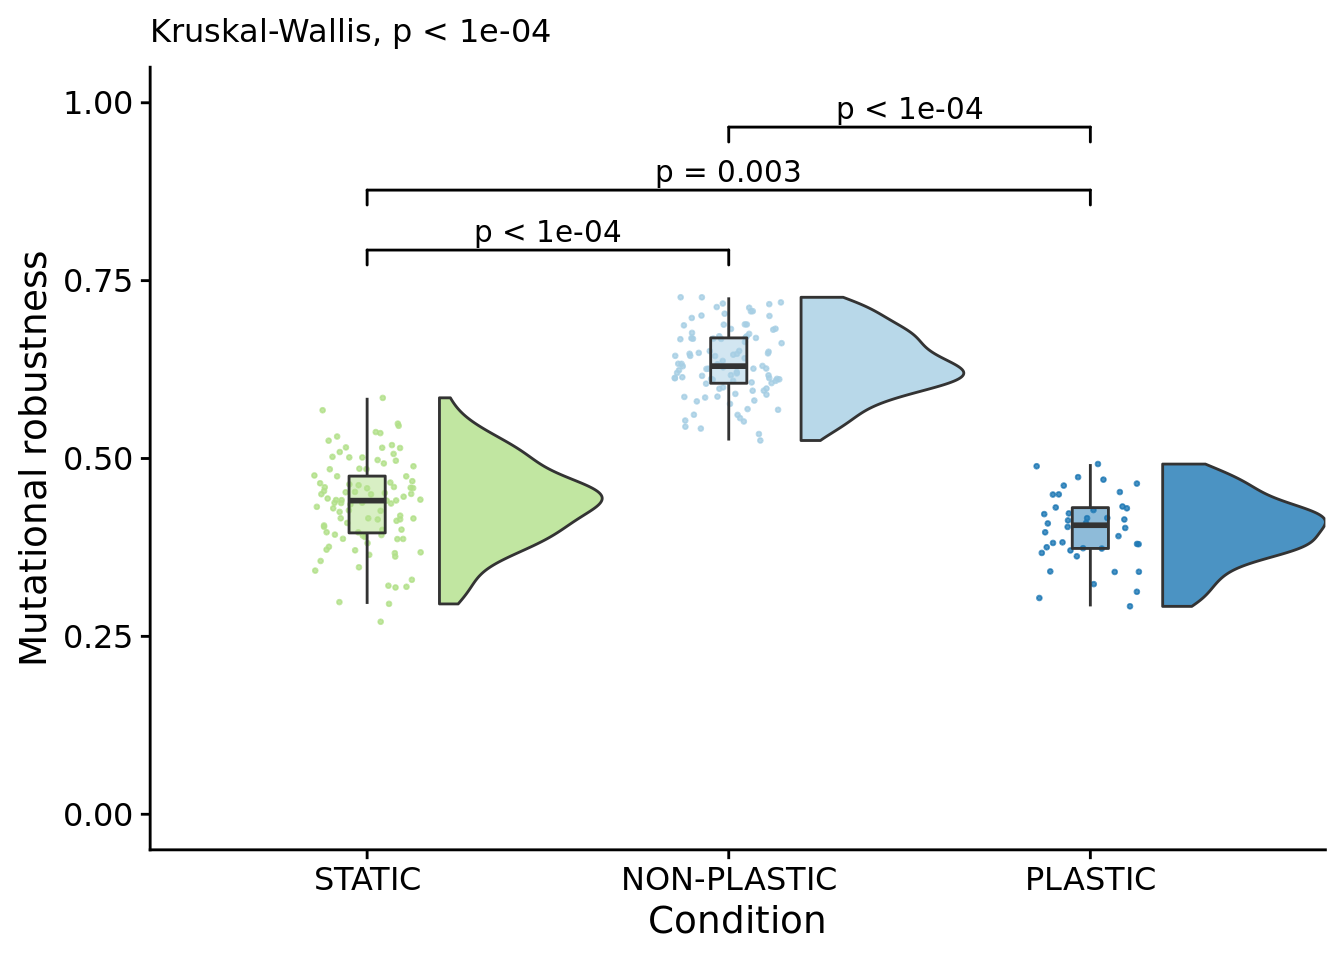
\includegraphics{supplemental-material_files/figure-latex/unnamed-chunk-42-1.pdf}

\begin{Shaded}
\begin{Highlighting}[]
\NormalTok{bo <-}\StringTok{ }\KeywordTok{boot}\NormalTok{(}\KeywordTok{filter}\NormalTok{(summary_data, condition}\OperatorTok{==}\StringTok{"PLASTIC"} \OperatorTok{&}\StringTok{ }\NormalTok{dominant_lineage_num_mut_steps_that_change_aggregate_phenotype }\OperatorTok{>}\StringTok{ }\DecValTok{0}\NormalTok{)}\OperatorTok{$}\NormalTok{frac_unexpressed_deleterious_mut_steps, }\DataTypeTok{statistic=}\NormalTok{samplemean, }\DataTypeTok{R=}\DecValTok{10000}\NormalTok{)}
\KeywordTok{print}\NormalTok{(bo)}
\end{Highlighting}
\end{Shaded}

\begin{verbatim}
## 
## ORDINARY NONPARAMETRIC BOOTSTRAP
## 
## 
## Call:
## boot(data = filter(summary_data, condition == "PLASTIC" & dominant_lineage_num_mut_steps_that_change_aggregate_phenotype > 
##     0)$frac_unexpressed_deleterious_mut_steps, statistic = samplemean, 
##     R = 10000)
## 
## 
## Bootstrap Statistics :
##      original        bias    std. error
## t1* 0.5172414 -0.0005206897  0.03977468
\end{verbatim}

\begin{Shaded}
\begin{Highlighting}[]
\KeywordTok{print}\NormalTok{(}\KeywordTok{boot.ci}\NormalTok{(bo, }\DataTypeTok{conf=}\FloatTok{0.95}\NormalTok{, }\DataTypeTok{type=}\StringTok{"perc"}\NormalTok{))}
\end{Highlighting}
\end{Shaded}

\begin{verbatim}
## BOOTSTRAP CONFIDENCE INTERVAL CALCULATIONS
## Based on 10000 bootstrap replicates
## 
## CALL : 
## boot.ci(boot.out = bo, conf = 0.95, type = "perc")
## 
## Intervals : 
## Level     Percentile     
## 95%   ( 0.4403,  0.5966 )  
## Calculations and Intervals on Original Scale
\end{verbatim}

Beneficial

\begin{Shaded}
\begin{Highlighting}[]
\NormalTok{summary_data}\OperatorTok{$}\NormalTok{frac_unexpressed_beneficial_mut_steps <-}\StringTok{ }\NormalTok{summary_data}\OperatorTok{$}\NormalTok{dominant_lineage_num_mut_steps_that_change_unexpressed_phenotype_beneficial }\OperatorTok{/}\StringTok{ }\NormalTok{summary_data}\OperatorTok{$}\NormalTok{dominant_lineage_num_mut_steps_that_change_unexpressed_phenotype}

\KeywordTok{ggplot}\NormalTok{(}
  \KeywordTok{filter}\NormalTok{(summary_data, condition}\OperatorTok{==}\StringTok{"PLASTIC"} \OperatorTok{&}\StringTok{ }\NormalTok{dominant_lineage_num_mut_steps_that_change_unexpressed_phenotype }\OperatorTok{>}\StringTok{ }\DecValTok{0}\NormalTok{),}
  \KeywordTok{aes}\NormalTok{(}\DataTypeTok{x=}\NormalTok{frac_unexpressed_beneficial_mut_steps)}
\NormalTok{  ) }\OperatorTok{+}
\StringTok{  }\KeywordTok{geom_density}\NormalTok{() }\OperatorTok{+}
\StringTok{  }\KeywordTok{theme}\NormalTok{(}
    \DataTypeTok{legend.position=}\StringTok{"none"}
\NormalTok{  )}
\end{Highlighting}
\end{Shaded}

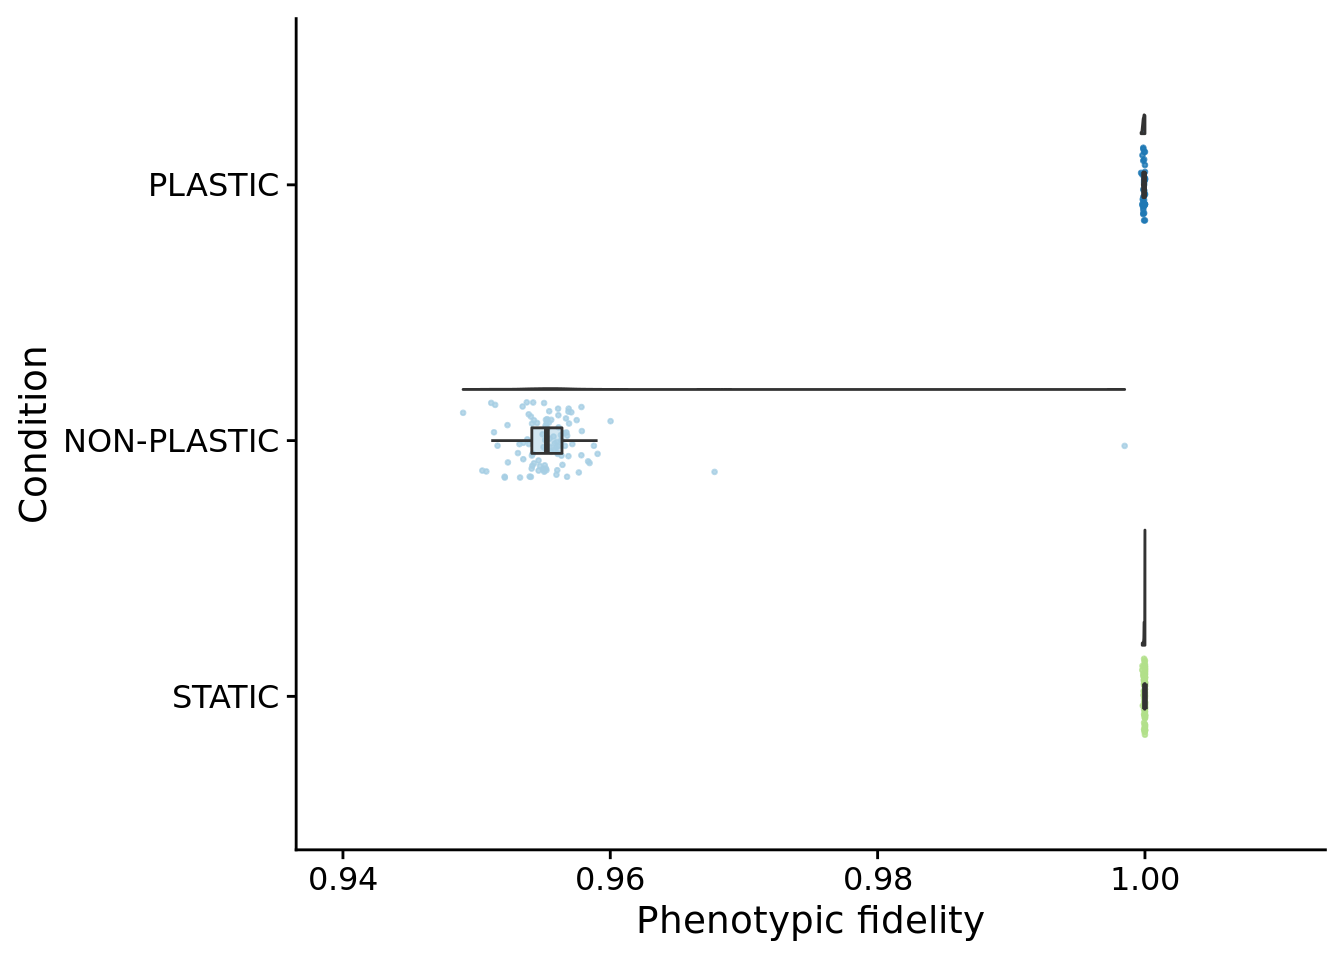
\includegraphics{supplemental-material_files/figure-latex/unnamed-chunk-43-1.pdf}

\begin{Shaded}
\begin{Highlighting}[]
\NormalTok{bo <-}\StringTok{ }\KeywordTok{boot}\NormalTok{(}\KeywordTok{filter}\NormalTok{(summary_data, condition}\OperatorTok{==}\StringTok{"PLASTIC"} \OperatorTok{&}\StringTok{ }\NormalTok{dominant_lineage_num_mut_steps_that_change_aggregate_phenotype }\OperatorTok{>}\StringTok{ }\DecValTok{0}\NormalTok{)}\OperatorTok{$}\NormalTok{frac_unexpressed_beneficial_mut_steps, }\DataTypeTok{statistic=}\NormalTok{samplemean, }\DataTypeTok{R=}\DecValTok{10000}\NormalTok{)}
\KeywordTok{print}\NormalTok{(bo)}
\end{Highlighting}
\end{Shaded}

\begin{verbatim}
## 
## ORDINARY NONPARAMETRIC BOOTSTRAP
## 
## 
## Call:
## boot(data = filter(summary_data, condition == "PLASTIC" & dominant_lineage_num_mut_steps_that_change_aggregate_phenotype > 
##     0)$frac_unexpressed_beneficial_mut_steps, statistic = samplemean, 
##     R = 10000)
## 
## 
## Bootstrap Statistics :
##      original      bias    std. error
## t1* 0.4827586 0.000111954  0.03932112
\end{verbatim}

\begin{Shaded}
\begin{Highlighting}[]
\KeywordTok{print}\NormalTok{(}\KeywordTok{boot.ci}\NormalTok{(bo, }\DataTypeTok{conf=}\FloatTok{0.95}\NormalTok{, }\DataTypeTok{type=}\StringTok{"perc"}\NormalTok{))}
\end{Highlighting}
\end{Shaded}

\begin{verbatim}
## BOOTSTRAP CONFIDENCE INTERVAL CALCULATIONS
## Based on 10000 bootstrap replicates
## 
## CALL : 
## boot.ci(boot.out = bo, conf = 0.95, type = "perc")
## 
## Intervals : 
## Level     Percentile     
## 95%   ( 0.4046,  0.5598 )  
## Calculations and Intervals on Original Scale
\end{verbatim}

\hypertarget{depth-of-mrca}{%
\section{Depth of MRCA}\label{depth-of-mrca}}

\begin{Shaded}
\begin{Highlighting}[]
\KeywordTok{ggplot}\NormalTok{(summary_data, }\KeywordTok{aes}\NormalTok{(}\DataTypeTok{x=}\NormalTok{condition, }\DataTypeTok{y=}\NormalTok{phylo_mrca_depth, }\DataTypeTok{fill=}\NormalTok{condition)) }\OperatorTok{+}
\StringTok{  }\KeywordTok{geom_flat_violin}\NormalTok{(}
    \DataTypeTok{position =} \KeywordTok{position_nudge}\NormalTok{(}\DataTypeTok{x =} \FloatTok{.2}\NormalTok{, }\DataTypeTok{y =} \DecValTok{0}\NormalTok{),}
    \DataTypeTok{alpha =} \FloatTok{.8}
\NormalTok{  ) }\OperatorTok{+}
\StringTok{  }\KeywordTok{geom_point}\NormalTok{(}
    \DataTypeTok{mapping=}\KeywordTok{aes}\NormalTok{(}\DataTypeTok{color=}\NormalTok{condition),}
    \DataTypeTok{position =} \KeywordTok{position_jitter}\NormalTok{(}\DataTypeTok{width =} \FloatTok{.15}\NormalTok{),}
    \DataTypeTok{size =} \FloatTok{.5}\NormalTok{,}
    \DataTypeTok{alpha =} \FloatTok{0.8}
\NormalTok{  ) }\OperatorTok{+}
\StringTok{  }\KeywordTok{geom_boxplot}\NormalTok{(}
    \DataTypeTok{width =} \FloatTok{.1}\NormalTok{,}
    \DataTypeTok{outlier.shape =} \OtherTok{NA}\NormalTok{,}
    \DataTypeTok{alpha =} \FloatTok{0.5}
\NormalTok{  ) }\OperatorTok{+}
\StringTok{  }\KeywordTok{scale_x_discrete}\NormalTok{(}
    \DataTypeTok{name=}\StringTok{"Condition"}\NormalTok{,}
    \DataTypeTok{limits=}\NormalTok{condition_order}
\NormalTok{  ) }\OperatorTok{+}
\StringTok{  }\KeywordTok{ylab}\NormalTok{(}\StringTok{"MRCA Depth"}\NormalTok{) }\OperatorTok{+}
\StringTok{  }\KeywordTok{theme}\NormalTok{(}
    \DataTypeTok{legend.position=}\StringTok{"none"}
\NormalTok{  )}
\end{Highlighting}
\end{Shaded}

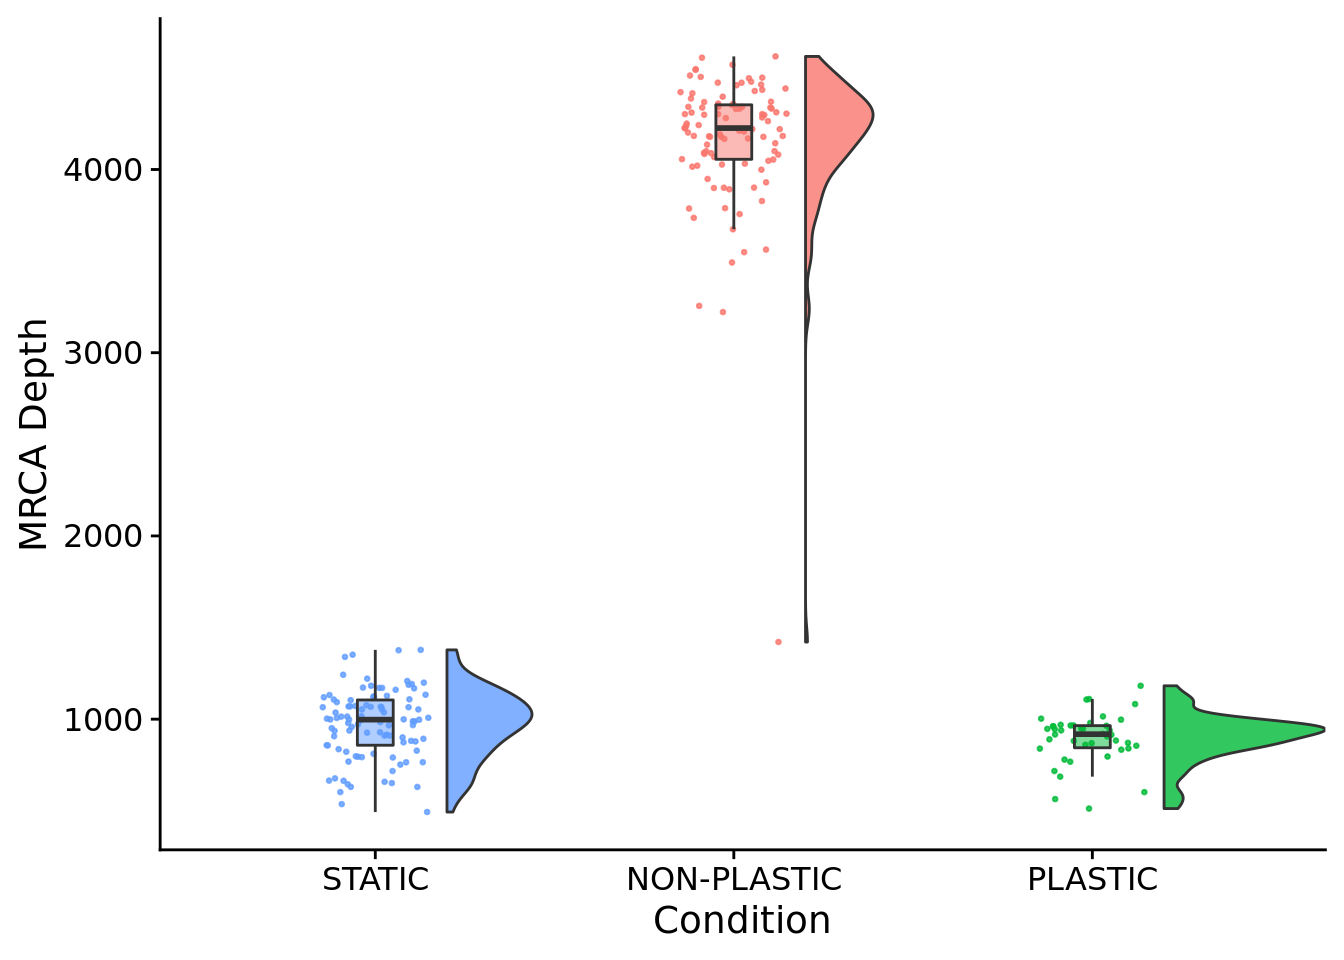
\includegraphics{supplemental-material_files/figure-latex/unnamed-chunk-44-1.pdf}

\hypertarget{manuscript-figures}{%
\section{Manuscript figures}\label{manuscript-figures}}

Figures styled for the paper.

\hypertarget{evolutionary-change-panel}{%
\subsection{Evolutionary change panel}\label{evolutionary-change-panel}}

Selective sweeps, mutation accumulation, phenotypic volatility.

Mutation accumulation:

\begin{Shaded}
\begin{Highlighting}[]
\CommentTok{# dominant_lineage_total_mut_cnt or mutations_per_lineage_step?}
\NormalTok{mutation_count_fig <-}\StringTok{ }\KeywordTok{ggplot}\NormalTok{(}
\NormalTok{    summary_data,}
    \KeywordTok{aes}\NormalTok{(}\DataTypeTok{x=}\NormalTok{condition, }\DataTypeTok{y=}\NormalTok{dominant_lineage_total_mut_cnt, }\DataTypeTok{fill=}\NormalTok{condition)}
\NormalTok{  ) }\OperatorTok{+}
\StringTok{  }\KeywordTok{geom_flat_violin}\NormalTok{(}
    \DataTypeTok{position =} \KeywordTok{position_nudge}\NormalTok{(}\DataTypeTok{x =} \FloatTok{.2}\NormalTok{, }\DataTypeTok{y =} \DecValTok{0}\NormalTok{),}
    \DataTypeTok{alpha =} \FloatTok{.8}
\NormalTok{  ) }\OperatorTok{+}
\StringTok{  }\KeywordTok{geom_point}\NormalTok{(}
    \DataTypeTok{mapping=}\KeywordTok{aes}\NormalTok{(}\DataTypeTok{color=}\NormalTok{condition),}
    \DataTypeTok{position =} \KeywordTok{position_jitter}\NormalTok{(}\DataTypeTok{width =} \FloatTok{.15}\NormalTok{),}
    \DataTypeTok{size =} \FloatTok{.5}\NormalTok{,}
    \DataTypeTok{alpha =} \FloatTok{0.8}
\NormalTok{  ) }\OperatorTok{+}
\StringTok{  }\KeywordTok{geom_boxplot}\NormalTok{(}
    \DataTypeTok{width =} \FloatTok{.1}\NormalTok{,}
    \DataTypeTok{outlier.shape =} \OtherTok{NA}\NormalTok{,}
    \DataTypeTok{alpha =} \FloatTok{0.5}
\NormalTok{  ) }\OperatorTok{+}
\StringTok{  }\KeywordTok{scale_x_discrete}\NormalTok{(}
    \DataTypeTok{name=}\StringTok{"Condition"}\NormalTok{,}
    \DataTypeTok{limits=}\NormalTok{condition_order,}
    \DataTypeTok{labels=}\NormalTok{condition_order}
\NormalTok{  ) }\OperatorTok{+}
\StringTok{  }\KeywordTok{scale_y_continuous}\NormalTok{(}
    \DataTypeTok{name=}\StringTok{"Mutations accumulated (log scale)"}\NormalTok{,}
    \DataTypeTok{trans=}\StringTok{"log10"}\NormalTok{,}
    \DataTypeTok{breaks=}\KeywordTok{c}\NormalTok{(}\DecValTok{100}\NormalTok{, }\DecValTok{1000}\NormalTok{, }\DecValTok{10000}\NormalTok{),}
    \DataTypeTok{limits=}\KeywordTok{c}\NormalTok{(}\DecValTok{100}\NormalTok{, }\DecValTok{10000}\NormalTok{)}
\NormalTok{  ) }\OperatorTok{+}
\StringTok{  }\KeywordTok{scale_fill_brewer}\NormalTok{(}
    \DataTypeTok{palette=}\StringTok{"Paired"}
\NormalTok{  ) }\OperatorTok{+}
\StringTok{  }\KeywordTok{scale_color_brewer}\NormalTok{(}
    \DataTypeTok{palette=}\StringTok{"Paired"}
\NormalTok{  ) }\OperatorTok{+}
\StringTok{  }\KeywordTok{coord_flip}\NormalTok{() }\OperatorTok{+}
\StringTok{  }\KeywordTok{theme}\NormalTok{(}
    \DataTypeTok{legend.position=}\StringTok{"none"}
\NormalTok{  ) }\OperatorTok{+}
\StringTok{  }\KeywordTok{ggsave}\NormalTok{(}
    \KeywordTok{paste0}\NormalTok{(working_directory, }\StringTok{"plots/"}\NormalTok{, }\StringTok{"mutation-accumulation.pdf"}\NormalTok{),}
    \DataTypeTok{width=}\DecValTok{5}\NormalTok{,}
    \DataTypeTok{height=}\DecValTok{4}
\NormalTok{  )}
\NormalTok{mutation_count_fig}
\end{Highlighting}
\end{Shaded}

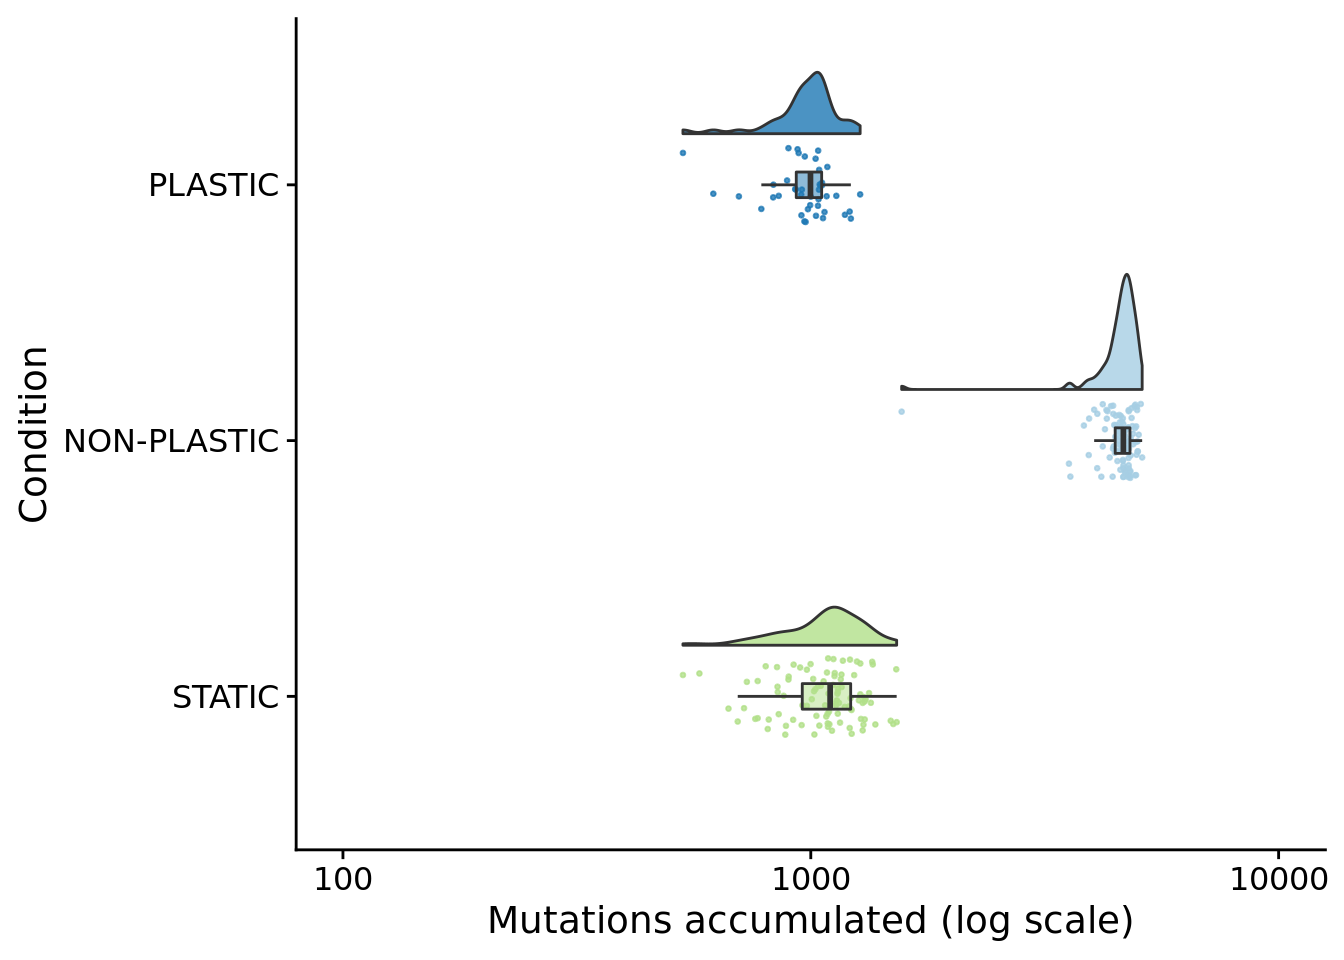
\includegraphics{supplemental-material_files/figure-latex/unnamed-chunk-45-1.pdf}

Phenotypic volatility:

\begin{Shaded}
\begin{Highlighting}[]
\NormalTok{phenotypic_volatility_fig <-}\StringTok{ }\KeywordTok{ggplot}\NormalTok{(}
\NormalTok{    summary_data,}
    \KeywordTok{aes}\NormalTok{(}\DataTypeTok{x=}\NormalTok{condition, }\DataTypeTok{y=}\NormalTok{dominant_lineage_trait_volatility, }\DataTypeTok{fill=}\NormalTok{condition)}
\NormalTok{  ) }\OperatorTok{+}
\StringTok{  }\KeywordTok{geom_flat_violin}\NormalTok{(}
    \DataTypeTok{position =} \KeywordTok{position_nudge}\NormalTok{(}\DataTypeTok{x =} \FloatTok{.2}\NormalTok{, }\DataTypeTok{y =} \DecValTok{0}\NormalTok{),}
    \DataTypeTok{alpha =} \FloatTok{.8}
\NormalTok{  ) }\OperatorTok{+}
\StringTok{  }\KeywordTok{geom_point}\NormalTok{(}
    \DataTypeTok{mapping=}\KeywordTok{aes}\NormalTok{(}\DataTypeTok{color=}\NormalTok{condition),}
    \DataTypeTok{position =} \KeywordTok{position_jitter}\NormalTok{(}\DataTypeTok{width =} \FloatTok{.15}\NormalTok{),}
    \DataTypeTok{size =} \FloatTok{.5}\NormalTok{,}
    \DataTypeTok{alpha =} \FloatTok{0.8}
\NormalTok{  ) }\OperatorTok{+}
\StringTok{  }\KeywordTok{geom_boxplot}\NormalTok{(}
    \DataTypeTok{width =} \FloatTok{.1}\NormalTok{,}
    \DataTypeTok{outlier.shape =} \OtherTok{NA}\NormalTok{,}
    \DataTypeTok{alpha =} \FloatTok{0.5}
\NormalTok{  ) }\OperatorTok{+}
\StringTok{  }\KeywordTok{scale_x_discrete}\NormalTok{(}
    \DataTypeTok{name=}\StringTok{"Condition"}\NormalTok{,}
    \DataTypeTok{limits=}\NormalTok{condition_order,}
    \DataTypeTok{labels=}\NormalTok{condition_order}
\NormalTok{  ) }\OperatorTok{+}
\StringTok{  }\KeywordTok{scale_y_continuous}\NormalTok{(}
    \DataTypeTok{name=}\StringTok{"Phenotypic volatility (log scale)"}\NormalTok{,}
    \DataTypeTok{trans=}\StringTok{"pseudo_log"}\NormalTok{,}
    \DataTypeTok{breaks=}\KeywordTok{c}\NormalTok{(}\DecValTok{0}\NormalTok{, }\DecValTok{10}\NormalTok{, }\DecValTok{100}\NormalTok{, }\DecValTok{1000}\NormalTok{, }\DecValTok{10000}\NormalTok{),}
    \DataTypeTok{limits=}\KeywordTok{c}\NormalTok{(}\OperatorTok{-}\DecValTok{1}\NormalTok{,}\DecValTok{10000}\NormalTok{)}
\NormalTok{  ) }\OperatorTok{+}
\StringTok{  }\KeywordTok{scale_fill_brewer}\NormalTok{(}
    \DataTypeTok{palette=}\StringTok{"Paired"}
\NormalTok{  ) }\OperatorTok{+}
\StringTok{  }\KeywordTok{scale_color_brewer}\NormalTok{(}
    \DataTypeTok{palette=}\StringTok{"Paired"}
\NormalTok{  ) }\OperatorTok{+}
\StringTok{  }\KeywordTok{coord_flip}\NormalTok{() }\OperatorTok{+}
\StringTok{  }\KeywordTok{theme}\NormalTok{(}
    \DataTypeTok{legend.position=}\StringTok{"none"}
\NormalTok{  ) }\OperatorTok{+}
\StringTok{  }\KeywordTok{ggsave}\NormalTok{(}
    \KeywordTok{paste0}\NormalTok{(working_directory, }\StringTok{"plots/"}\NormalTok{, }\StringTok{"phenotypic-volatility.pdf"}\NormalTok{),}
    \DataTypeTok{width=}\DecValTok{4}\NormalTok{,}
    \DataTypeTok{height=}\DecValTok{4}
\NormalTok{  )}

\NormalTok{phenotypic_volatility_fig}
\end{Highlighting}
\end{Shaded}

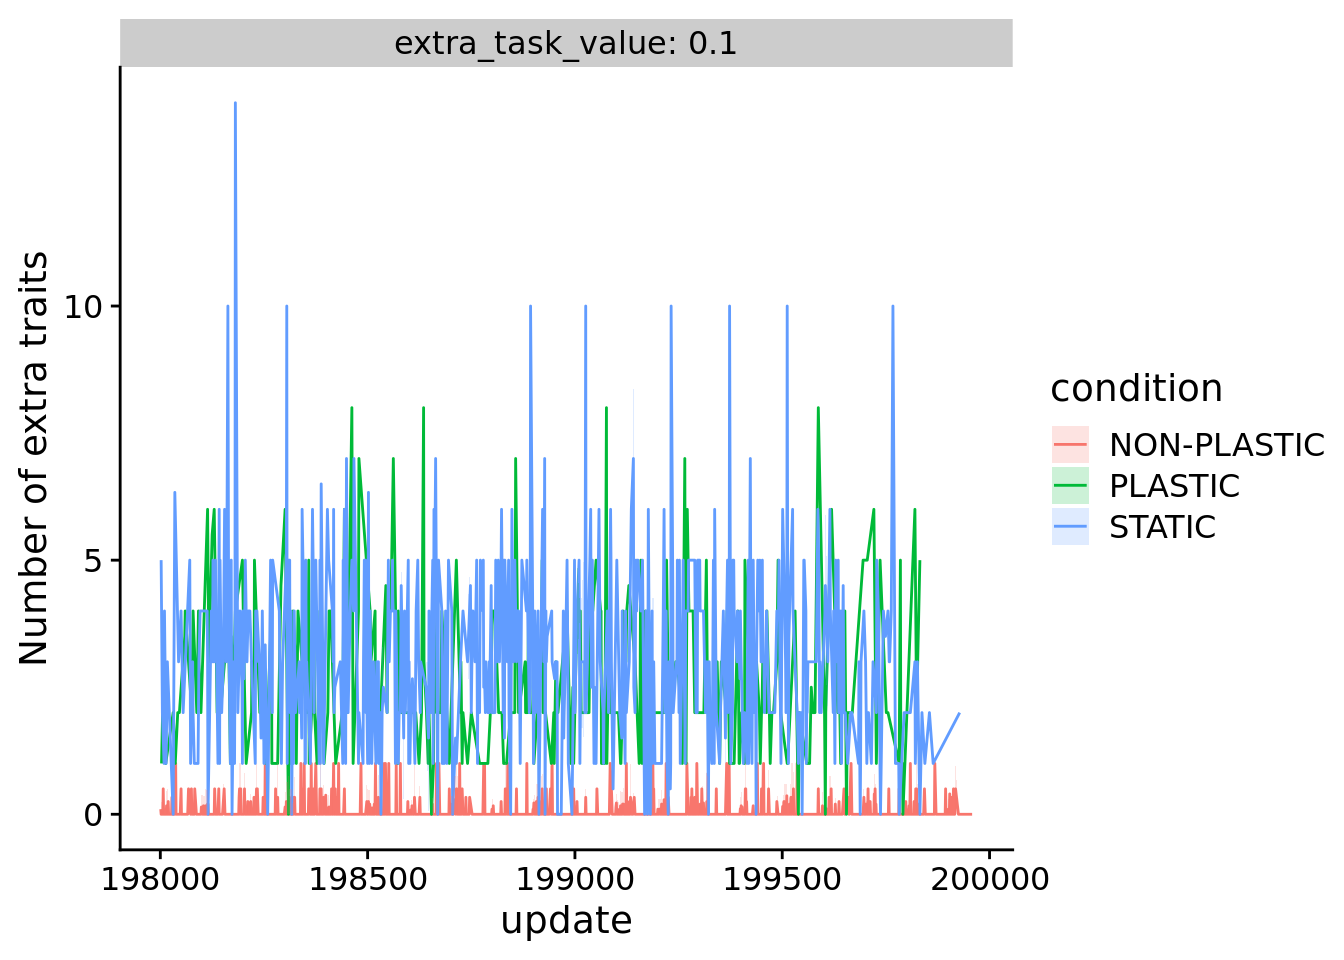
\includegraphics{supplemental-material_files/figure-latex/unnamed-chunk-46-1.pdf}

Selective sweeps:

\begin{Shaded}
\begin{Highlighting}[]
\NormalTok{selective_sweeps_fig <-}\StringTok{ }\KeywordTok{ggplot}\NormalTok{(}
\NormalTok{    summary_data,}
    \KeywordTok{aes}\NormalTok{(}\DataTypeTok{x=}\NormalTok{condition, }\DataTypeTok{y=}\NormalTok{phylo_mrca_changes, }\DataTypeTok{fill=}\NormalTok{condition)}
\NormalTok{  ) }\OperatorTok{+}
\StringTok{  }\KeywordTok{geom_flat_violin}\NormalTok{(}
    \DataTypeTok{position =} \KeywordTok{position_nudge}\NormalTok{(}\DataTypeTok{x =} \FloatTok{.2}\NormalTok{, }\DataTypeTok{y =} \DecValTok{0}\NormalTok{),}
    \DataTypeTok{alpha =} \FloatTok{.8}
\NormalTok{  ) }\OperatorTok{+}
\StringTok{  }\KeywordTok{geom_point}\NormalTok{(}
    \DataTypeTok{mapping=}\KeywordTok{aes}\NormalTok{(}\DataTypeTok{color=}\NormalTok{condition),}
    \DataTypeTok{position =} \KeywordTok{position_jitter}\NormalTok{(}\DataTypeTok{width =} \FloatTok{.15}\NormalTok{),}
    \DataTypeTok{size =} \FloatTok{.5}\NormalTok{,}
    \DataTypeTok{alpha =} \FloatTok{0.8}
\NormalTok{  ) }\OperatorTok{+}
\StringTok{  }\KeywordTok{geom_boxplot}\NormalTok{(}
    \DataTypeTok{width =} \FloatTok{.1}\NormalTok{,}
    \DataTypeTok{outlier.shape =} \OtherTok{NA}\NormalTok{,}
    \DataTypeTok{alpha =} \FloatTok{0.5}
\NormalTok{  ) }\OperatorTok{+}
\StringTok{  }\KeywordTok{scale_x_discrete}\NormalTok{(}
    \DataTypeTok{name=}\StringTok{"Condition"}\NormalTok{,}
    \DataTypeTok{limits=}\NormalTok{condition_order,}
    \DataTypeTok{labels=}\NormalTok{condition_order}
\NormalTok{  ) }\OperatorTok{+}
\StringTok{  }\KeywordTok{scale_y_continuous}\NormalTok{(}
    \DataTypeTok{name=}\StringTok{"Coalescence Events (log scale)"}\NormalTok{,}
    \DataTypeTok{trans=}\StringTok{"log10"}\NormalTok{,}
    \DataTypeTok{breaks=}\KeywordTok{c}\NormalTok{(}\DecValTok{10}\NormalTok{, }\DecValTok{100}\NormalTok{, }\DecValTok{1000}\NormalTok{),}
    \DataTypeTok{limits=}\KeywordTok{c}\NormalTok{(}\DecValTok{10}\NormalTok{, }\DecValTok{1000}\NormalTok{)}
\NormalTok{  ) }\OperatorTok{+}
\StringTok{  }\KeywordTok{scale_fill_brewer}\NormalTok{(}
    \DataTypeTok{palette=}\StringTok{"Paired"}
\NormalTok{  ) }\OperatorTok{+}
\StringTok{  }\KeywordTok{scale_color_brewer}\NormalTok{(}
    \DataTypeTok{palette=}\StringTok{"Paired"}
\NormalTok{  ) }\OperatorTok{+}
\StringTok{  }\KeywordTok{coord_flip}\NormalTok{() }\OperatorTok{+}
\StringTok{  }\KeywordTok{theme}\NormalTok{(}
    \DataTypeTok{legend.position=}\StringTok{"none"}
\NormalTok{  ) }\OperatorTok{+}
\StringTok{  }\KeywordTok{ggsave}\NormalTok{(}
    \KeywordTok{paste0}\NormalTok{(working_directory, }\StringTok{"plots/"}\NormalTok{, }\StringTok{"selective-sweeps.pdf"}\NormalTok{),}
    \DataTypeTok{width=}\DecValTok{4}\NormalTok{,}
    \DataTypeTok{height=}\DecValTok{4}
\NormalTok{  )}

\NormalTok{selective_sweeps_fig}
\end{Highlighting}
\end{Shaded}

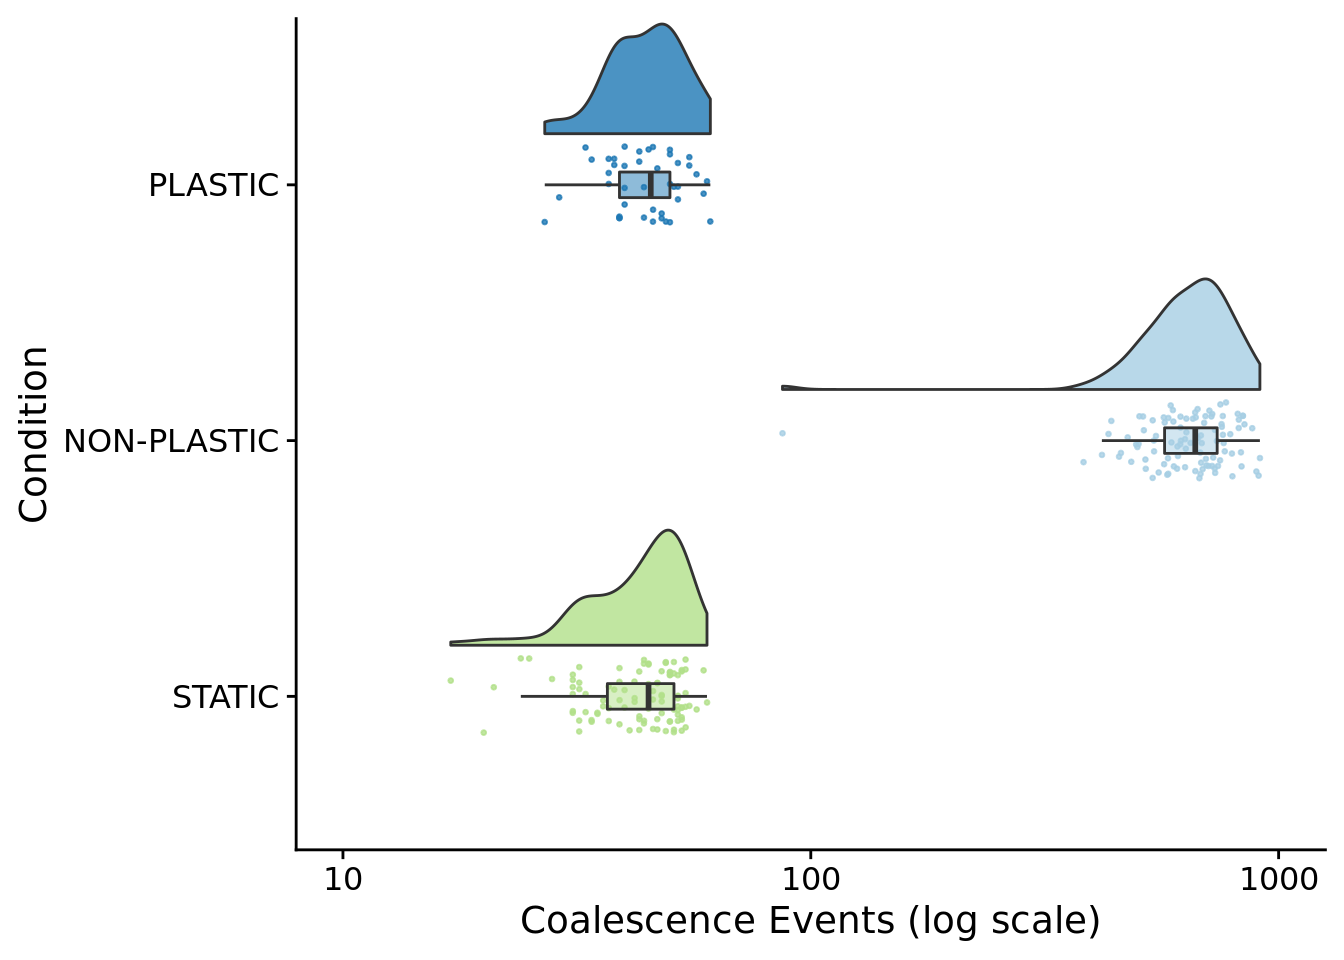
\includegraphics{supplemental-material_files/figure-latex/unnamed-chunk-47-1.pdf}

All together:

\begin{Shaded}
\begin{Highlighting}[]
\NormalTok{grid <-}\StringTok{ }\KeywordTok{plot_grid}\NormalTok{(}
\NormalTok{  selective_sweeps_fig }\OperatorTok{+}\StringTok{ }\KeywordTok{theme}\NormalTok{(}
    \DataTypeTok{legend.position=}\StringTok{"none"}
\NormalTok{  ),}
\NormalTok{  mutation_count_fig }\OperatorTok{+}\StringTok{ }\KeywordTok{theme}\NormalTok{(}
    \DataTypeTok{legend.position=}\StringTok{"none"}\NormalTok{,}
    \DataTypeTok{axis.ticks.y=}\KeywordTok{element_blank}\NormalTok{(),}
    \DataTypeTok{axis.text.y=}\KeywordTok{element_blank}\NormalTok{(),}
    \DataTypeTok{axis.title.y=}\KeywordTok{element_blank}\NormalTok{()}
\NormalTok{  ),}
\NormalTok{  phenotypic_volatility_fig }\OperatorTok{+}\StringTok{ }\KeywordTok{theme}\NormalTok{(}
    \DataTypeTok{legend.position=}\StringTok{"none"}\NormalTok{,}
    \DataTypeTok{axis.ticks.y=}\KeywordTok{element_blank}\NormalTok{(),}
    \DataTypeTok{axis.text.y=}\KeywordTok{element_blank}\NormalTok{(),}
    \DataTypeTok{axis.title.y=}\KeywordTok{element_blank}\NormalTok{()}
\NormalTok{  ),}
  \DataTypeTok{nrow=}\DecValTok{1}\NormalTok{,}
  \DataTypeTok{align=}\StringTok{"v"}\NormalTok{,}
  \DataTypeTok{labels=}\StringTok{"auto"}
\NormalTok{)}
\NormalTok{grid}
\end{Highlighting}
\end{Shaded}

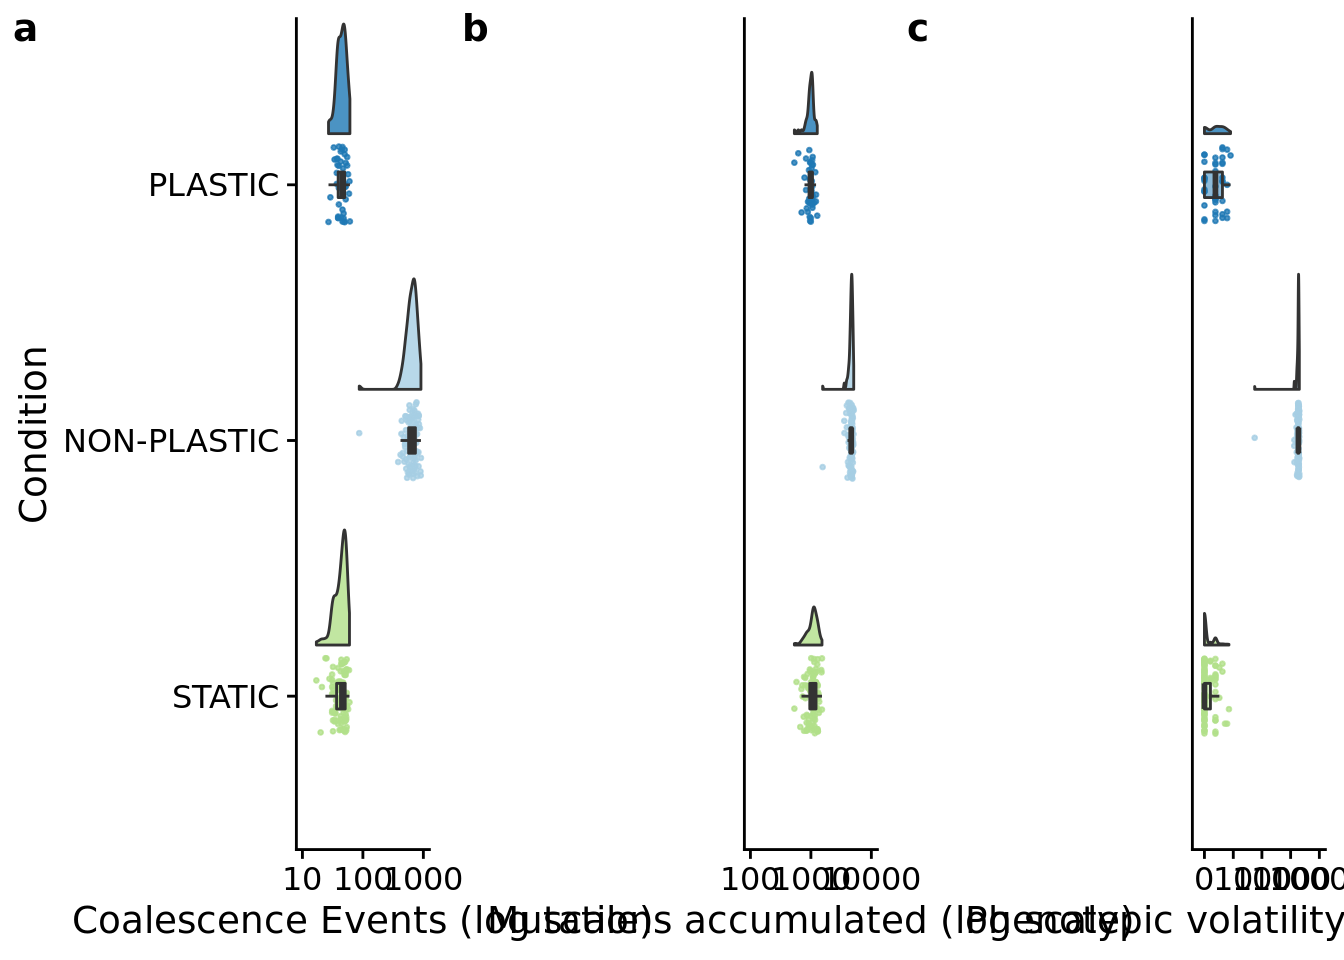
\includegraphics{supplemental-material_files/figure-latex/unnamed-chunk-48-1.pdf}

\begin{Shaded}
\begin{Highlighting}[]
\KeywordTok{save_plot}\NormalTok{(}
   \KeywordTok{paste0}\NormalTok{(working_directory, }\StringTok{"plots/"}\NormalTok{, }\StringTok{"evolutionary-dynamics.pdf"}\NormalTok{),}
\NormalTok{   grid,}
   \DataTypeTok{base_height=}\DecValTok{6}\NormalTok{,}
   \DataTypeTok{base_asp=}\FloatTok{2.5}
\NormalTok{)}
\end{Highlighting}
\end{Shaded}

\hypertarget{evolution-and-maintenance-of-novel-traits}{%
\chapter{Evolution and maintenance of novel traits}\label{evolution-and-maintenance-of-novel-traits}}

The effect of adaptive phenotypic plasticity on the evolution and maintenance of novel traits.

\hypertarget{overview-2}{%
\section{Overview}\label{overview-2}}

\begin{Shaded}
\begin{Highlighting}[]
\NormalTok{total_updates <-}\StringTok{ }\DecValTok{200000}
\NormalTok{replicates <-}\StringTok{ }\DecValTok{100}

\NormalTok{focal_traits <-}\StringTok{ }\KeywordTok{c}\NormalTok{(}\StringTok{"not"}\NormalTok{,}\StringTok{"nand"}\NormalTok{,}\StringTok{"and"}\NormalTok{,}\StringTok{"ornot"}\NormalTok{,}\StringTok{"or"}\NormalTok{,}\StringTok{"andnot"}\NormalTok{)}
\NormalTok{traits_set_a <-}\StringTok{ }\KeywordTok{c}\NormalTok{(}\StringTok{"not"}\NormalTok{, }\StringTok{"and"}\NormalTok{, }\StringTok{"or"}\NormalTok{)}
\NormalTok{traits_set_b <-}\StringTok{ }\KeywordTok{c}\NormalTok{(}\StringTok{"nand"}\NormalTok{, }\StringTok{"ornot"}\NormalTok{, }\StringTok{"andnot"}\NormalTok{)}
\NormalTok{extra_traits <-}\StringTok{ }\KeywordTok{c}\NormalTok{(}
  \StringTok{"nor"}\NormalTok{,}\StringTok{"xor"}\NormalTok{,}\StringTok{"equals"}\NormalTok{,}
  \StringTok{"logic_3aa"}\NormalTok{,}\StringTok{"logic_3ab"}\NormalTok{,}\StringTok{"logic_3ac"}\NormalTok{,}
  \StringTok{"logic_3ad"}\NormalTok{,}\StringTok{"logic_3ae"}\NormalTok{,}\StringTok{"logic_3af"}\NormalTok{,}
  \StringTok{"logic_3ag"}\NormalTok{,}\StringTok{"logic_3ah"}\NormalTok{,}\StringTok{"logic_3ai"}\NormalTok{,}
  \StringTok{"logic_3aj"}\NormalTok{,}\StringTok{"logic_3ak"}\NormalTok{,}\StringTok{"logic_3al"}\NormalTok{,}
  \StringTok{"logic_3am"}\NormalTok{,}\StringTok{"logic_3an"}\NormalTok{,}\StringTok{"logic_3ao"}\NormalTok{,}
  \StringTok{"logic_3ap"}\NormalTok{,}\StringTok{"logic_3aq"}\NormalTok{,}\StringTok{"logic_3ar"}\NormalTok{,}
  \StringTok{"logic_3as"}\NormalTok{,}\StringTok{"logic_3at"}\NormalTok{,}\StringTok{"logic_3au"}\NormalTok{,}
  \StringTok{"logic_3av"}\NormalTok{,}\StringTok{"logic_3aw"}\NormalTok{,}\StringTok{"logic_3ax"}\NormalTok{,}
  \StringTok{"logic_3ay"}\NormalTok{,}\StringTok{"logic_3az"}\NormalTok{,}\StringTok{"logic_3ba"}\NormalTok{,}
  \StringTok{"logic_3bb"}\NormalTok{,}\StringTok{"logic_3bc"}\NormalTok{,}\StringTok{"logic_3bd"}\NormalTok{,}
  \StringTok{"logic_3be"}\NormalTok{,}\StringTok{"logic_3bf"}\NormalTok{,}\StringTok{"logic_3bg"}\NormalTok{,}
  \StringTok{"logic_3bh"}\NormalTok{,}\StringTok{"logic_3bi"}\NormalTok{,}\StringTok{"logic_3bj"}\NormalTok{,}
  \StringTok{"logic_3bk"}\NormalTok{,}\StringTok{"logic_3bl"}\NormalTok{,}\StringTok{"logic_3bm"}\NormalTok{,}
  \StringTok{"logic_3bn"}\NormalTok{,}\StringTok{"logic_3bo"}\NormalTok{,}\StringTok{"logic_3bp"}\NormalTok{,}
  \StringTok{"logic_3bq"}\NormalTok{,}\StringTok{"logic_3br"}\NormalTok{,}\StringTok{"logic_3bs"}\NormalTok{,}
  \StringTok{"logic_3bt"}\NormalTok{,}\StringTok{"logic_3bu"}\NormalTok{,}\StringTok{"logic_3bv"}\NormalTok{,}
  \StringTok{"logic_3bw"}\NormalTok{,}\StringTok{"logic_3bx"}\NormalTok{,}\StringTok{"logic_3by"}\NormalTok{,}
  \StringTok{"logic_3bz"}\NormalTok{,}\StringTok{"logic_3ca"}\NormalTok{,}\StringTok{"logic_3cb"}\NormalTok{,}
  \StringTok{"logic_3cc"}\NormalTok{,}\StringTok{"logic_3cd"}\NormalTok{,}\StringTok{"logic_3ce"}\NormalTok{,}
  \StringTok{"logic_3cf"}\NormalTok{,}\StringTok{"logic_3cg"}\NormalTok{,}\StringTok{"logic_3ch"}\NormalTok{,}
  \StringTok{"logic_3ci"}\NormalTok{,}\StringTok{"logic_3cj"}\NormalTok{,}\StringTok{"logic_3ck"}\NormalTok{,}
  \StringTok{"logic_3cl"}\NormalTok{,}\StringTok{"logic_3cm"}\NormalTok{,}\StringTok{"logic_3cn"}\NormalTok{,}
  \StringTok{"logic_3co"}\NormalTok{,}\StringTok{"logic_3cp"}
\NormalTok{)}

\CommentTok{# Relative location of data.}
\NormalTok{working_directory <-}\StringTok{ "experiments/2021-01-31-complex-features/analysis/"} \CommentTok{# << For bookdown}
\CommentTok{# working_directory <- "./"}
\end{Highlighting}
\end{Shaded}

\hypertarget{analysis-dependencies-2}{%
\section{Analysis dependencies}\label{analysis-dependencies-2}}

Load all required R libraries.

\begin{Shaded}
\begin{Highlighting}[]
\KeywordTok{library}\NormalTok{(ggplot2)}
\KeywordTok{library}\NormalTok{(tidyverse)}
\KeywordTok{library}\NormalTok{(cowplot)}
\KeywordTok{library}\NormalTok{(RColorBrewer)}
\KeywordTok{library}\NormalTok{(Hmisc)}
\KeywordTok{library}\NormalTok{(boot)}
\KeywordTok{source}\NormalTok{(}\StringTok{"https://gist.githubusercontent.com/benmarwick/2a1bb0133ff568cbe28d/raw/fb53bd97121f7f9ce947837ef1a4c65a73bffb3f/geom_flat_violin.R"}\NormalTok{)}
\end{Highlighting}
\end{Shaded}

These analyses were conducted/knitted with the following computing environment:

\begin{Shaded}
\begin{Highlighting}[]
\KeywordTok{print}\NormalTok{(version)}
\end{Highlighting}
\end{Shaded}

\begin{verbatim}
##                _                           
## platform       x86_64-pc-linux-gnu         
## arch           x86_64                      
## os             linux-gnu                   
## system         x86_64, linux-gnu           
## status                                     
## major          4                           
## minor          0.4                         
## year           2021                        
## month          02                          
## day            15                          
## svn rev        80002                       
## language       R                           
## version.string R version 4.0.4 (2021-02-15)
## nickname       Lost Library Book
\end{verbatim}

\hypertarget{setup-2}{%
\section{Setup}\label{setup-2}}

\begin{Shaded}
\begin{Highlighting}[]
\CommentTok{####### summary data #######}
\NormalTok{summary_data_loc <-}\StringTok{ }\KeywordTok{paste0}\NormalTok{(working_directory, }\StringTok{"data/aggregate.csv"}\NormalTok{)}
\NormalTok{summary_data <-}\StringTok{ }\KeywordTok{read.csv}\NormalTok{(summary_data_loc, }\DataTypeTok{na.strings=}\StringTok{"NONE"}\NormalTok{)}

\NormalTok{summary_data}\OperatorTok{$}\NormalTok{DISABLE_REACTION_SENSORS <-}\StringTok{ }\KeywordTok{as.factor}\NormalTok{(summary_data}\OperatorTok{$}\NormalTok{DISABLE_REACTION_SENSORS)}
\NormalTok{summary_data}\OperatorTok{$}\NormalTok{chg_env <-}\StringTok{ }\NormalTok{summary_data}\OperatorTok{$}\NormalTok{chg_env }\OperatorTok{==}\StringTok{ "True"}
\NormalTok{summary_data}\OperatorTok{$}\NormalTok{dominant_plastic_odd_even <-}\StringTok{ }\KeywordTok{as.factor}\NormalTok{(summary_data}\OperatorTok{$}\NormalTok{dominant_plastic_odd_even)}
\NormalTok{summary_data}\OperatorTok{$}\NormalTok{sensors <-}\StringTok{ }\NormalTok{summary_data}\OperatorTok{$}\NormalTok{DISABLE_REACTION_SENSORS }\OperatorTok{==}\StringTok{ "0"}
\NormalTok{summary_data}\OperatorTok{$}\NormalTok{is_plastic <-}\StringTok{ }\NormalTok{summary_data}\OperatorTok{$}\NormalTok{dominant_plastic_odd_even }\OperatorTok{==}\StringTok{ "True"}
\NormalTok{summary_data}\OperatorTok{$}\NormalTok{extra_task_value <-}\StringTok{ }\KeywordTok{as.factor}\NormalTok{(summary_data}\OperatorTok{$}\NormalTok{extra_task_value)}
\NormalTok{summary_data <-}\StringTok{ }\KeywordTok{filter}\NormalTok{(summary_data, extra_task_value }\OperatorTok{==}\StringTok{ }\FloatTok{0.1}\NormalTok{)}

\NormalTok{env_label_fun <-}\StringTok{ }\ControlFlowTok{function}\NormalTok{(chg_env) \{}
  \ControlFlowTok{if}\NormalTok{ (chg_env) \{}
    \KeywordTok{return}\NormalTok{(}\StringTok{"Fluctuating"}\NormalTok{)}
\NormalTok{  \} }\ControlFlowTok{else}\NormalTok{ \{}
    \KeywordTok{return}\NormalTok{(}\StringTok{"Constant"}\NormalTok{)}
\NormalTok{  \}}
\NormalTok{\}}

\NormalTok{sensors_label_fun <-}\StringTok{ }\ControlFlowTok{function}\NormalTok{(has_sensors) \{}
  \ControlFlowTok{if}\NormalTok{ (has_sensors) \{}
    \KeywordTok{return}\NormalTok{(}\StringTok{"Sensors"}\NormalTok{)}
\NormalTok{  \} }\ControlFlowTok{else}\NormalTok{ \{}
    \KeywordTok{return}\NormalTok{(}\StringTok{"No sensors"}\NormalTok{)}
\NormalTok{  \}}
\NormalTok{\}}

\NormalTok{condition_label_fun <-}\StringTok{ }\ControlFlowTok{function}\NormalTok{(has_sensors, env_chg) \{}
  \ControlFlowTok{if}\NormalTok{ (has_sensors }\OperatorTok{&&}\StringTok{ }\NormalTok{env_chg) \{}
    \KeywordTok{return}\NormalTok{(}\StringTok{"PLASTIC"}\NormalTok{)}
\NormalTok{  \} }\ControlFlowTok{else} \ControlFlowTok{if}\NormalTok{ (env_chg) \{}
    \KeywordTok{return}\NormalTok{(}\StringTok{"NON-PLASTIC"}\NormalTok{)}
\NormalTok{  \} }\ControlFlowTok{else}\NormalTok{ \{}
    \KeywordTok{return}\NormalTok{(}\StringTok{"STATIC"}\NormalTok{)}
\NormalTok{  \}}
\NormalTok{\}}

\NormalTok{summary_data}\OperatorTok{$}\NormalTok{env_label <-}\StringTok{ }\KeywordTok{mapply}\NormalTok{(}
\NormalTok{  env_label_fun,}
\NormalTok{  summary_data}\OperatorTok{$}\NormalTok{chg_env}
\NormalTok{)}
\NormalTok{summary_data}\OperatorTok{$}\NormalTok{sensors_label <-}\StringTok{ }\KeywordTok{mapply}\NormalTok{(}
\NormalTok{  sensors_label_fun,}
\NormalTok{  summary_data}\OperatorTok{$}\NormalTok{sensors}
\NormalTok{)}
\NormalTok{summary_data}\OperatorTok{$}\NormalTok{condition <-}\StringTok{ }\KeywordTok{mapply}\NormalTok{(}
\NormalTok{  condition_label_fun,}
\NormalTok{  summary_data}\OperatorTok{$}\NormalTok{sensors,}
\NormalTok{  summary_data}\OperatorTok{$}\NormalTok{chg_env}
\NormalTok{)}

\NormalTok{condition_order =}\StringTok{ }\KeywordTok{c}\NormalTok{(}
  \StringTok{"STATIC"}\NormalTok{,}
  \StringTok{"NON-PLASTIC"}\NormalTok{,}
  \StringTok{"PLASTIC"}
\NormalTok{)}

\CommentTok{###### time series #####}
\NormalTok{lineage_time_series_data_loc <-}\StringTok{ }\KeywordTok{paste0}\NormalTok{(working_directory, }\StringTok{"data/lineage_series.csv"}\NormalTok{)}
\NormalTok{lineage_time_series_data <-}\StringTok{ }\KeywordTok{read.csv}\NormalTok{(lineage_time_series_data_loc)}

\NormalTok{lineage_time_series_data}\OperatorTok{$}\NormalTok{DISABLE_REACTION_SENSORS <-}\StringTok{ }\KeywordTok{as.factor}\NormalTok{(lineage_time_series_data}\OperatorTok{$}\NormalTok{DISABLE_REACTION_SENSORS)}
\NormalTok{lineage_time_series_data}\OperatorTok{$}\NormalTok{chg_env <-}\StringTok{ }\NormalTok{lineage_time_series_data}\OperatorTok{$}\NormalTok{chg_env }\OperatorTok{==}\StringTok{ "True"}
\NormalTok{lineage_time_series_data}\OperatorTok{$}\NormalTok{sensors <-}\StringTok{ }\NormalTok{lineage_time_series_data}\OperatorTok{$}\NormalTok{DISABLE_REACTION_SENSORS }\OperatorTok{==}\StringTok{ "0"}
\NormalTok{lineage_time_series_data}\OperatorTok{$}\NormalTok{extra_task_value <-}\StringTok{ }\KeywordTok{as.factor}\NormalTok{(lineage_time_series_data}\OperatorTok{$}\NormalTok{extra_task_value)}

\NormalTok{lineage_time_series_data}\OperatorTok{$}\NormalTok{env_label <-}\StringTok{ }\KeywordTok{mapply}\NormalTok{(}
\NormalTok{  env_label_fun,}
\NormalTok{  lineage_time_series_data}\OperatorTok{$}\NormalTok{chg_env}
\NormalTok{)}
\NormalTok{lineage_time_series_data}\OperatorTok{$}\NormalTok{sensors_label <-}\StringTok{ }\KeywordTok{mapply}\NormalTok{(}
\NormalTok{  sensors_label_fun,}
\NormalTok{  lineage_time_series_data}\OperatorTok{$}\NormalTok{sensors}
\NormalTok{)}
\NormalTok{lineage_time_series_data}\OperatorTok{$}\NormalTok{condition <-}\StringTok{ }\KeywordTok{mapply}\NormalTok{(}
\NormalTok{  condition_label_fun,}
\NormalTok{  lineage_time_series_data}\OperatorTok{$}\NormalTok{sensors,}
\NormalTok{  lineage_time_series_data}\OperatorTok{$}\NormalTok{chg_env}
\NormalTok{)}

\CommentTok{####### misc #######}
\CommentTok{# Configure our default graphing theme}
\KeywordTok{theme_set}\NormalTok{(}\KeywordTok{theme_cowplot}\NormalTok{())}
\KeywordTok{dir.create}\NormalTok{(}\KeywordTok{paste0}\NormalTok{(working_directory, }\StringTok{"plots"}\NormalTok{), }\DataTypeTok{showWarnings=}\OtherTok{FALSE}\NormalTok{)}
\end{Highlighting}
\end{Shaded}

\hypertarget{evolution-of-phenotypic-plasticity-2}{%
\section{Evolution of phenotypic plasticity}\label{evolution-of-phenotypic-plasticity-2}}

For sensor-enabled populations in fluctuating environments, we only transfered populations containing an optimally plastic genotype to phase two.

\begin{Shaded}
\begin{Highlighting}[]
\NormalTok{summary_data_grouped =}\StringTok{ }\NormalTok{dplyr}\OperatorTok{::}\KeywordTok{group_by}\NormalTok{(summary_data, sensors, env_label, condition, extra_task_value)}
\NormalTok{summary_data_group_counts =}\StringTok{ }\NormalTok{dplyr}\OperatorTok{::}\KeywordTok{summarize}\NormalTok{(summary_data_grouped, }\DataTypeTok{n=}\NormalTok{dplyr}\OperatorTok{::}\KeywordTok{n}\NormalTok{())}

\KeywordTok{ggplot}\NormalTok{(summary_data_group_counts, }\KeywordTok{aes}\NormalTok{(}\DataTypeTok{x=}\NormalTok{condition, }\DataTypeTok{y=}\NormalTok{n, }\DataTypeTok{fill=}\NormalTok{condition)) }\OperatorTok{+}
\StringTok{  }\KeywordTok{geom_col}\NormalTok{(}\DataTypeTok{position=}\KeywordTok{position_dodge}\NormalTok{(}\FloatTok{0.9}\NormalTok{)) }\OperatorTok{+}
\StringTok{  }\KeywordTok{geom_text}\NormalTok{(}\KeywordTok{aes}\NormalTok{(}\DataTypeTok{label=}\NormalTok{n, }\DataTypeTok{y=}\NormalTok{n}\OperatorTok{+}\DecValTok{2}\NormalTok{)) }\OperatorTok{+}
\StringTok{  }\KeywordTok{scale_x_discrete}\NormalTok{(}
    \DataTypeTok{name=}\StringTok{"Condition"}\NormalTok{,}
    \DataTypeTok{limits=}\NormalTok{condition_order}
\NormalTok{  ) }\OperatorTok{+}
\StringTok{  }\KeywordTok{ylab}\NormalTok{(}\StringTok{"Number of replicates in phase two"}\NormalTok{) }\OperatorTok{+}
\StringTok{  }\KeywordTok{facet_wrap}\NormalTok{(}\OperatorTok{~}\NormalTok{extra_task_value, }\DataTypeTok{labeller=}\NormalTok{label_both) }\OperatorTok{+}
\StringTok{  }\KeywordTok{theme}\NormalTok{(}
    \DataTypeTok{legend.position=}\StringTok{"none"}
\NormalTok{  )}
\end{Highlighting}
\end{Shaded}

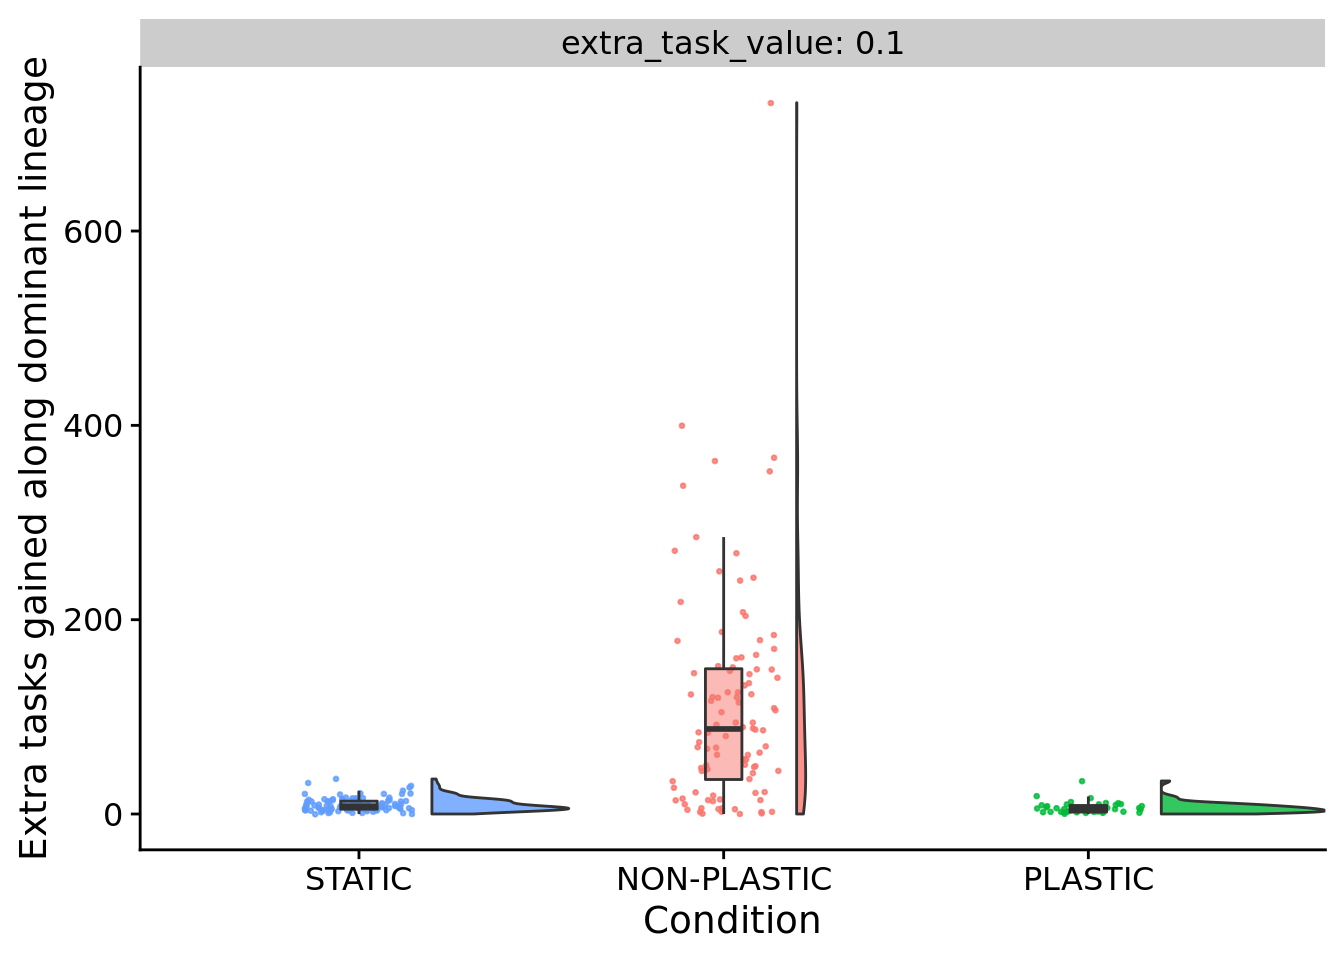
\includegraphics{supplemental-material_files/figure-latex/unnamed-chunk-53-1.pdf}

We can confirm our expectation that the dominant genotypes in non-plastic conditions are not phenotypically plastic.

\begin{Shaded}
\begin{Highlighting}[]
\NormalTok{summary_data_grouped =}\StringTok{ }\NormalTok{dplyr}\OperatorTok{::}\KeywordTok{group_by}\NormalTok{(summary_data, condition, is_plastic, extra_task_value)}
\NormalTok{summary_data_group_counts =}\StringTok{ }\NormalTok{dplyr}\OperatorTok{::}\KeywordTok{summarize}\NormalTok{(summary_data_grouped, }\DataTypeTok{n=}\NormalTok{dplyr}\OperatorTok{::}\KeywordTok{n}\NormalTok{())}
\KeywordTok{ggplot}\NormalTok{(}\KeywordTok{filter}\NormalTok{(summary_data_group_counts, is_plastic), }\KeywordTok{aes}\NormalTok{(}\DataTypeTok{x=}\NormalTok{condition, }\DataTypeTok{y=}\NormalTok{n, }\DataTypeTok{fill=}\NormalTok{condition)) }\OperatorTok{+}
\StringTok{  }\KeywordTok{geom_col}\NormalTok{(}\DataTypeTok{position=}\KeywordTok{position_dodge}\NormalTok{(}\FloatTok{0.9}\NormalTok{)) }\OperatorTok{+}
\StringTok{  }\KeywordTok{scale_x_discrete}\NormalTok{(}
    \DataTypeTok{name=}\StringTok{"Condition"}\NormalTok{,}
    \DataTypeTok{limits=}\NormalTok{condition_order}
\NormalTok{  ) }\OperatorTok{+}
\StringTok{  }\KeywordTok{ylim}\NormalTok{(}\DecValTok{0}\NormalTok{, }\DecValTok{100}\NormalTok{) }\OperatorTok{+}
\StringTok{  }\KeywordTok{geom_text}\NormalTok{(}\KeywordTok{aes}\NormalTok{(}\DataTypeTok{label=}\NormalTok{n, }\DataTypeTok{y=}\NormalTok{n}\OperatorTok{+}\DecValTok{1}\NormalTok{)) }\OperatorTok{+}
\StringTok{  }\KeywordTok{ylab}\NormalTok{(}\StringTok{"Number of replicates with a plastic dominant genotype"}\NormalTok{) }\OperatorTok{+}
\StringTok{  }\KeywordTok{facet_wrap}\NormalTok{(}\OperatorTok{~}\NormalTok{extra_task_value, }\DataTypeTok{labeller=}\NormalTok{label_both) }\OperatorTok{+}
\StringTok{  }\KeywordTok{theme}\NormalTok{(}
    \DataTypeTok{legend.position=}\StringTok{"none"}
\NormalTok{  )}
\end{Highlighting}
\end{Shaded}

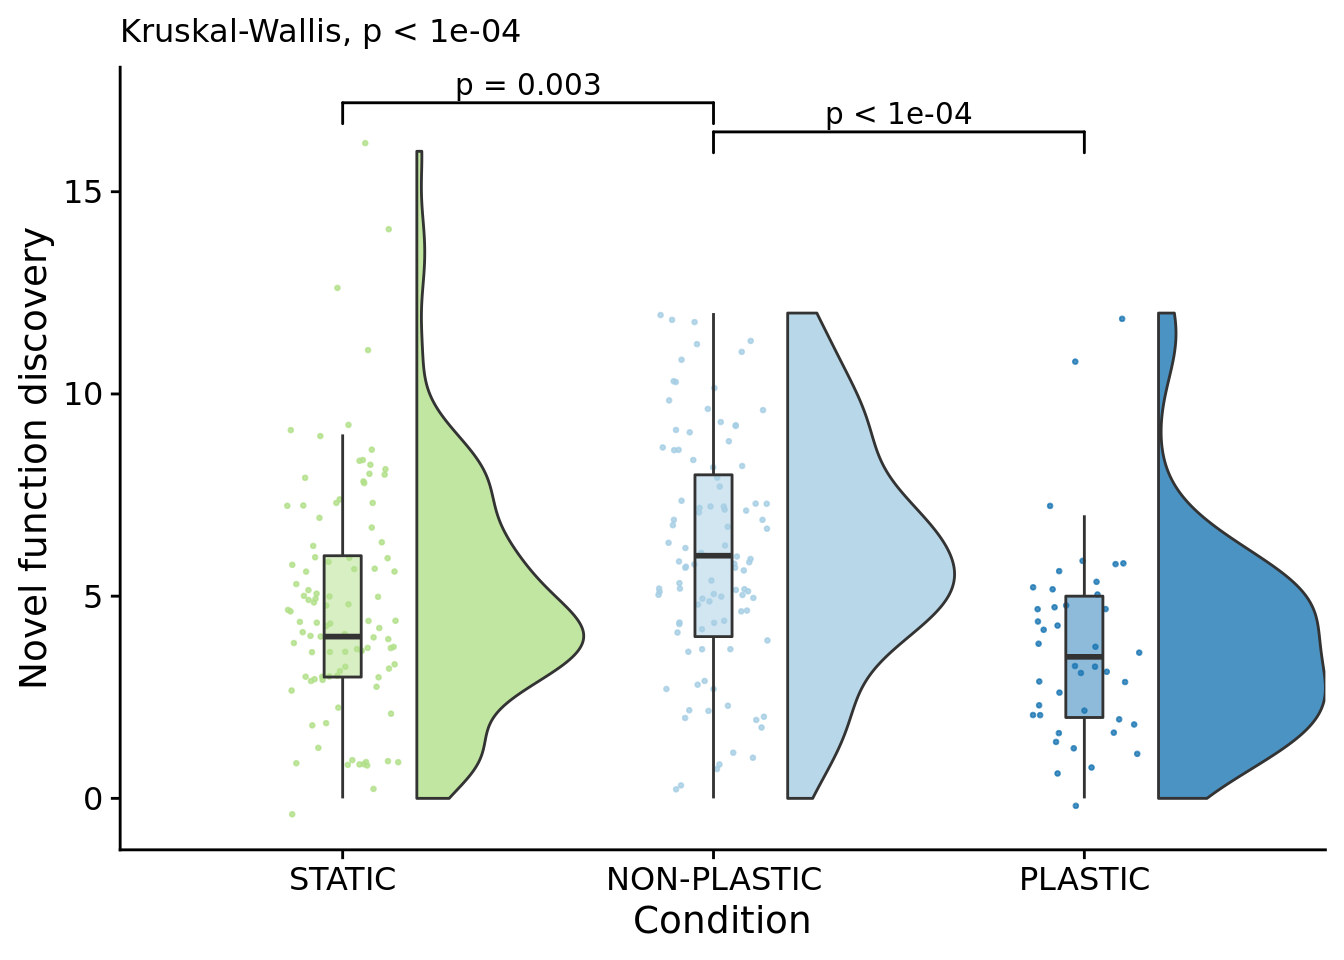
\includegraphics{supplemental-material_files/figure-latex/unnamed-chunk-54-1.pdf}

\hypertarget{final-dominant-novel-task-performance}{%
\section{Final dominant novel task performance}\label{final-dominant-novel-task-performance}}

How many novel tasks do final dominant genotypes perform?

\begin{Shaded}
\begin{Highlighting}[]
\KeywordTok{ggplot}\NormalTok{(summary_data, }\KeywordTok{aes}\NormalTok{(}\DataTypeTok{x=}\NormalTok{condition, }\DataTypeTok{y=}\NormalTok{dominant_extra_tasks, }\DataTypeTok{fill=}\NormalTok{condition)) }\OperatorTok{+}
\StringTok{  }\KeywordTok{geom_flat_violin}\NormalTok{(}
    \DataTypeTok{position =} \KeywordTok{position_nudge}\NormalTok{(}\DataTypeTok{x =} \FloatTok{.2}\NormalTok{, }\DataTypeTok{y =} \DecValTok{0}\NormalTok{),}
    \DataTypeTok{alpha =} \FloatTok{.8}
\NormalTok{  ) }\OperatorTok{+}
\StringTok{  }\KeywordTok{geom_point}\NormalTok{(}
    \DataTypeTok{mapping=}\KeywordTok{aes}\NormalTok{(}\DataTypeTok{color=}\NormalTok{condition),}
    \DataTypeTok{position =} \KeywordTok{position_jitter}\NormalTok{(}\DataTypeTok{width =} \FloatTok{.15}\NormalTok{),}
    \DataTypeTok{size =} \FloatTok{.5}\NormalTok{,}
    \DataTypeTok{alpha =} \FloatTok{0.8}
\NormalTok{  ) }\OperatorTok{+}
\StringTok{  }\KeywordTok{geom_boxplot}\NormalTok{(}
    \DataTypeTok{width =} \FloatTok{.1}\NormalTok{,}
    \DataTypeTok{outlier.shape =} \OtherTok{NA}\NormalTok{,}
    \DataTypeTok{alpha =} \FloatTok{0.5}
\NormalTok{  ) }\OperatorTok{+}
\StringTok{  }\KeywordTok{scale_x_discrete}\NormalTok{(}
    \DataTypeTok{name=}\StringTok{"Condition"}\NormalTok{,}
    \DataTypeTok{limits=}\NormalTok{condition_order}
\NormalTok{  ) }\OperatorTok{+}
\StringTok{  }\KeywordTok{ylab}\NormalTok{(}\StringTok{"Novel tasks performed by final dominant"}\NormalTok{) }\OperatorTok{+}
\StringTok{  }\KeywordTok{facet_wrap}\NormalTok{(}
    \OperatorTok{~}\NormalTok{extra_task_value,}
    \DataTypeTok{labeller=}\NormalTok{label_both}
\NormalTok{  ) }\OperatorTok{+}
\StringTok{  }\KeywordTok{theme}\NormalTok{(}
    \DataTypeTok{legend.position=}\StringTok{"none"}
\NormalTok{  ) }\OperatorTok{+}
\StringTok{  }\KeywordTok{ggsave}\NormalTok{(}
    \KeywordTok{paste0}\NormalTok{(working_directory, }\StringTok{"plots/dominant-extra-tasks.pdf"}\NormalTok{),}
    \DataTypeTok{width=}\DecValTok{15}\NormalTok{,}
    \DataTypeTok{height=}\DecValTok{10}
\NormalTok{  )}
\end{Highlighting}
\end{Shaded}

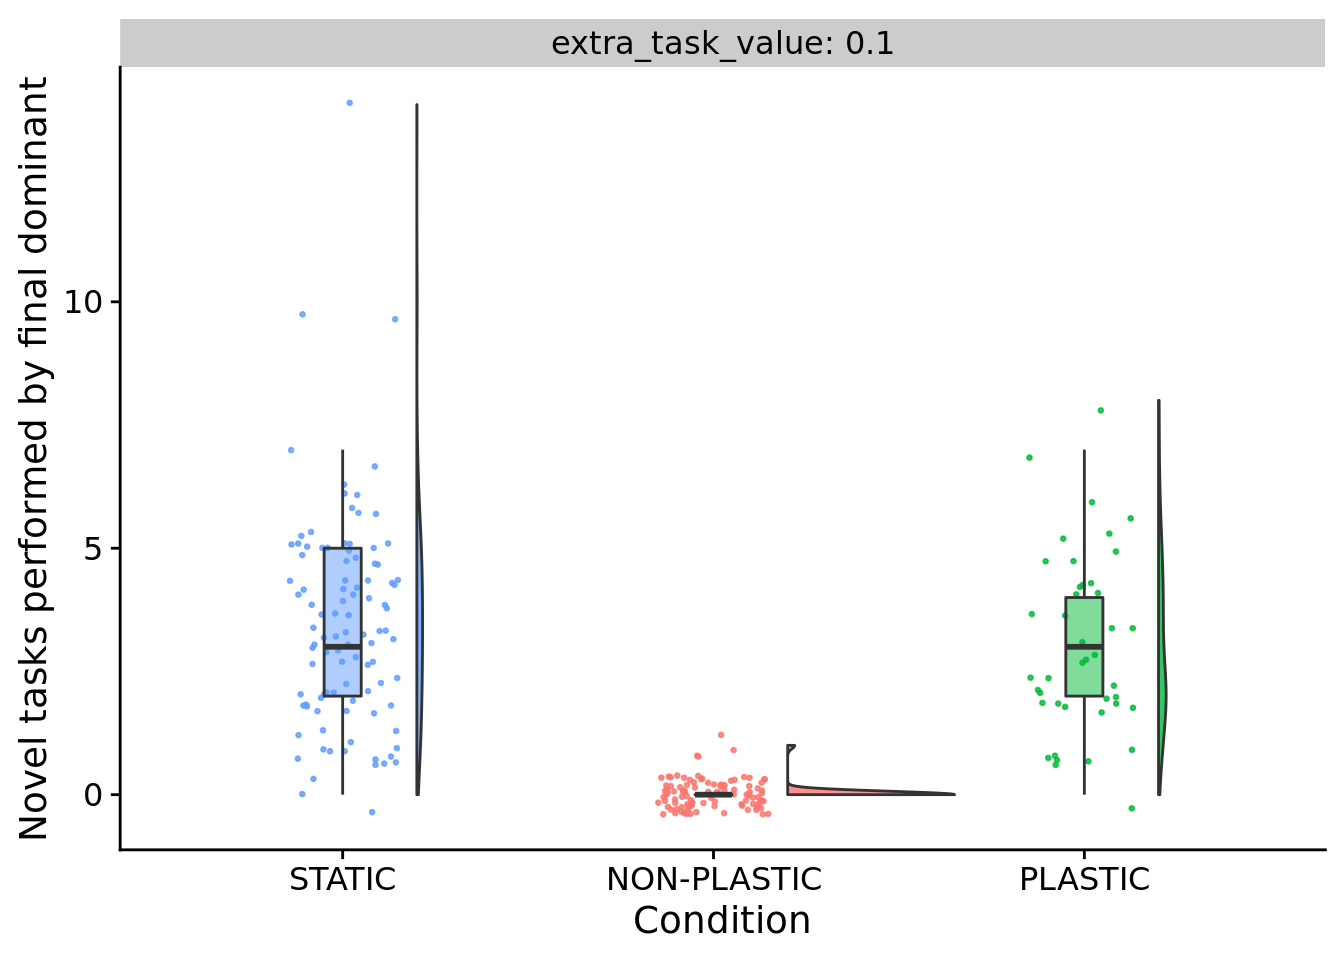
\includegraphics{supplemental-material_files/figure-latex/unnamed-chunk-55-1.pdf}

\begin{Shaded}
\begin{Highlighting}[]
\KeywordTok{paste0}\NormalTok{(}
  \StringTok{"PLASTIC median: "}\NormalTok{,}
  \KeywordTok{median}\NormalTok{(}\KeywordTok{filter}\NormalTok{(summary_data, condition}\OperatorTok{==}\StringTok{"PLASTIC"}\NormalTok{)}\OperatorTok{$}\NormalTok{dominant_extra_tasks)}
\NormalTok{)}
\end{Highlighting}
\end{Shaded}

\begin{verbatim}
## [1] "PLASTIC median: 3"
\end{verbatim}

\begin{Shaded}
\begin{Highlighting}[]
\KeywordTok{paste0}\NormalTok{(}
  \StringTok{"STATIC median: "}\NormalTok{,}
  \KeywordTok{median}\NormalTok{(}\KeywordTok{filter}\NormalTok{(summary_data, condition}\OperatorTok{==}\StringTok{"STATIC"}\NormalTok{)}\OperatorTok{$}\NormalTok{dominant_extra_tasks)}
\NormalTok{)}
\end{Highlighting}
\end{Shaded}

\begin{verbatim}
## [1] "STATIC median: 3"
\end{verbatim}

\begin{Shaded}
\begin{Highlighting}[]
\KeywordTok{paste0}\NormalTok{(}
  \StringTok{"NON-PLASTIC median: "}\NormalTok{,}
  \KeywordTok{median}\NormalTok{(}\KeywordTok{filter}\NormalTok{(summary_data, condition}\OperatorTok{==}\StringTok{"NON-PLASTIC"}\NormalTok{)}\OperatorTok{$}\NormalTok{dominant_extra_tasks)}
\NormalTok{)}
\end{Highlighting}
\end{Shaded}

\begin{verbatim}
## [1] "NON-PLASTIC median: 0"
\end{verbatim}

\begin{Shaded}
\begin{Highlighting}[]
\NormalTok{reward_level <-}\StringTok{ }\FloatTok{0.1}
\NormalTok{dom_task_data <-}\StringTok{ }\KeywordTok{filter}\NormalTok{(summary_data, extra_task_value}\OperatorTok{==}\NormalTok{reward_level)}
\KeywordTok{kruskal.test}\NormalTok{(}
  \DataTypeTok{formula=}\NormalTok{dominant_extra_tasks}\OperatorTok{~}\NormalTok{condition,}
  \DataTypeTok{data=}\NormalTok{dom_task_data}
\NormalTok{)}
\end{Highlighting}
\end{Shaded}

\begin{verbatim}
## 
##  Kruskal-Wallis rank sum test
## 
## data:  dominant_extra_tasks by condition
## Kruskal-Wallis chi-squared = 177.17, df = 2, p-value < 2.2e-16
\end{verbatim}

\begin{Shaded}
\begin{Highlighting}[]
\KeywordTok{pairwise.wilcox.test}\NormalTok{(}
  \DataTypeTok{x=}\NormalTok{dom_task_data}\OperatorTok{$}\NormalTok{dominant_extra_tasks,}
  \DataTypeTok{g=}\NormalTok{dom_task_data}\OperatorTok{$}\NormalTok{condition,}
  \DataTypeTok{p.adjust.method=}\StringTok{"bonferroni"}\NormalTok{,}
  \DataTypeTok{conf.int=}\OtherTok{TRUE}\NormalTok{,}
  \DataTypeTok{conf.level=}\FloatTok{0.95}
\NormalTok{)}
\end{Highlighting}
\end{Shaded}

\begin{verbatim}
## 
##  Pairwise comparisons using Wilcoxon rank sum test with continuity correction 
## 
## data:  dom_task_data$dominant_extra_tasks and dom_task_data$condition 
## 
##         NON-PLASTIC PLASTIC
## PLASTIC <2e-16      -      
## STATIC  <2e-16      0.9    
## 
## P value adjustment method: bonferroni
\end{verbatim}

\hypertarget{final-population-novel-task-performance}{%
\section{Final population novel task performance}\label{final-population-novel-task-performance}}

How many novel tasks are performed across the final population (1\% of organisms must perform to count)?

\begin{Shaded}
\begin{Highlighting}[]
\KeywordTok{ggplot}\NormalTok{(summary_data, }\KeywordTok{aes}\NormalTok{(}\DataTypeTok{x=}\NormalTok{condition, }\DataTypeTok{y=}\NormalTok{final_pop_extra_tasks_}\FloatTok{0.01}\NormalTok{, }\DataTypeTok{fill=}\NormalTok{condition)) }\OperatorTok{+}
\StringTok{  }\KeywordTok{geom_flat_violin}\NormalTok{(}
    \DataTypeTok{position =} \KeywordTok{position_nudge}\NormalTok{(}\DataTypeTok{x =} \FloatTok{.2}\NormalTok{, }\DataTypeTok{y =} \DecValTok{0}\NormalTok{),}
    \DataTypeTok{alpha =} \FloatTok{.8}
\NormalTok{  ) }\OperatorTok{+}
\StringTok{  }\KeywordTok{geom_point}\NormalTok{(}
    \DataTypeTok{mapping=}\KeywordTok{aes}\NormalTok{(}\DataTypeTok{color=}\NormalTok{condition),}
    \DataTypeTok{position =} \KeywordTok{position_jitter}\NormalTok{(}\DataTypeTok{width =} \FloatTok{.15}\NormalTok{),}
    \DataTypeTok{size =} \FloatTok{.5}\NormalTok{,}
    \DataTypeTok{alpha =} \FloatTok{0.8}
\NormalTok{  ) }\OperatorTok{+}
\StringTok{  }\KeywordTok{geom_boxplot}\NormalTok{(}
    \DataTypeTok{width =} \FloatTok{.1}\NormalTok{,}
    \DataTypeTok{outlier.shape =} \OtherTok{NA}\NormalTok{,}
    \DataTypeTok{alpha =} \FloatTok{0.5}
\NormalTok{  ) }\OperatorTok{+}
\StringTok{  }\KeywordTok{scale_x_discrete}\NormalTok{(}
    \DataTypeTok{name=}\StringTok{"Condition"}\NormalTok{,}
    \DataTypeTok{limits=}\NormalTok{condition_order}
\NormalTok{  ) }\OperatorTok{+}
\StringTok{  }\KeywordTok{facet_wrap}\NormalTok{(}
    \OperatorTok{~}\NormalTok{extra_task_value,}
    \DataTypeTok{labeller=}\NormalTok{label_both}
\NormalTok{  ) }\OperatorTok{+}
\StringTok{  }\KeywordTok{theme}\NormalTok{(}
    \DataTypeTok{legend.position=}\StringTok{"none"}
\NormalTok{  )}
\end{Highlighting}
\end{Shaded}

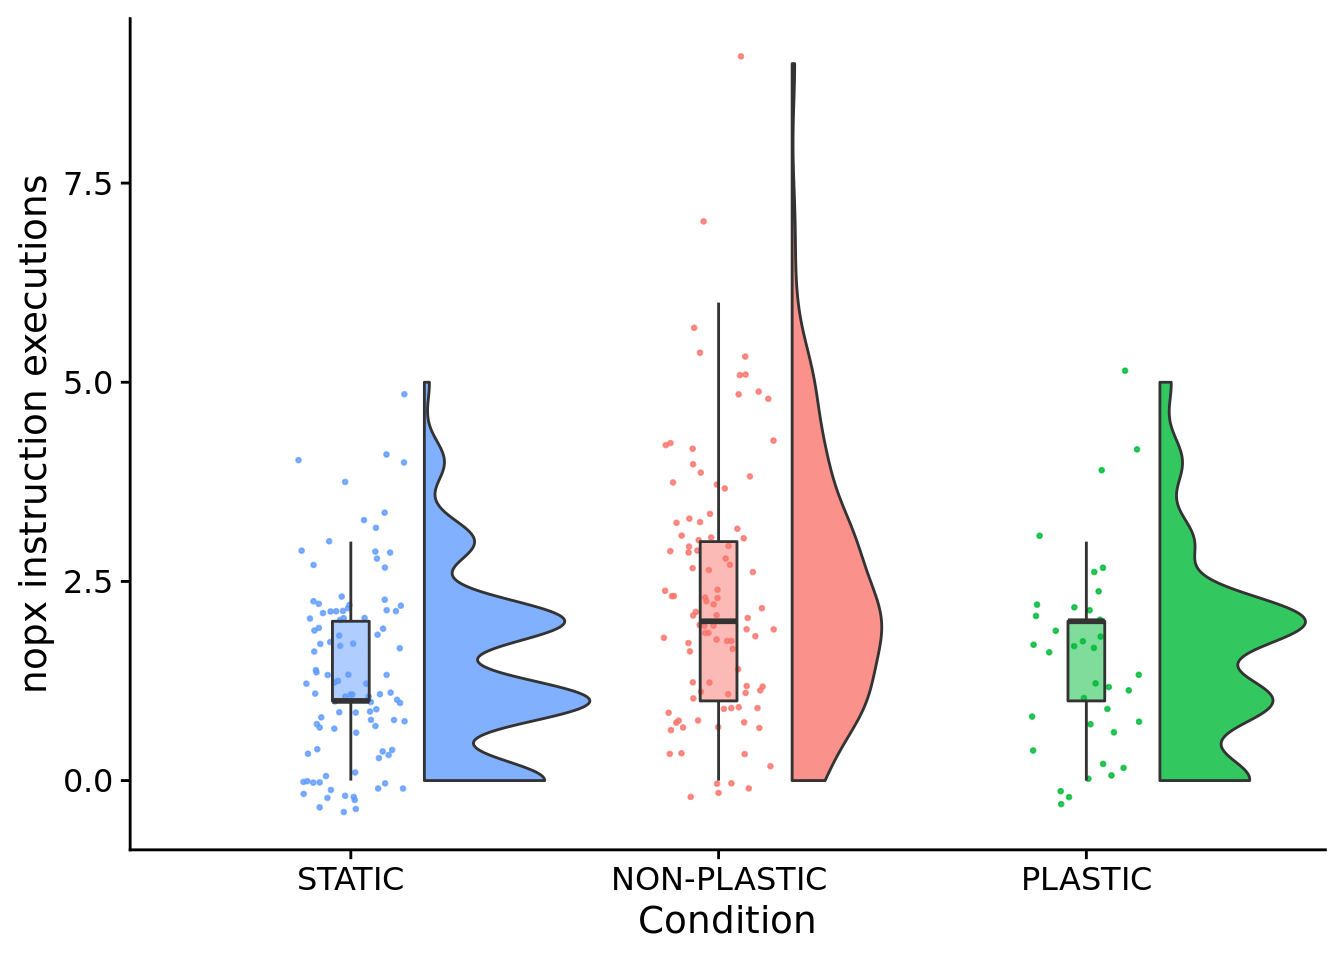
\includegraphics{supplemental-material_files/figure-latex/unnamed-chunk-57-1.pdf}

\begin{Shaded}
\begin{Highlighting}[]
\KeywordTok{paste0}\NormalTok{(}
  \StringTok{"PLASTIC median: "}\NormalTok{,}
  \KeywordTok{median}\NormalTok{(}\KeywordTok{filter}\NormalTok{(summary_data, condition}\OperatorTok{==}\StringTok{"PLASTIC"}\NormalTok{)}\OperatorTok{$}\NormalTok{final_pop_extra_tasks_}\FloatTok{0.01}\NormalTok{)}
\NormalTok{)}
\end{Highlighting}
\end{Shaded}

\begin{verbatim}
## [1] "PLASTIC median: 3"
\end{verbatim}

\begin{Shaded}
\begin{Highlighting}[]
\KeywordTok{paste0}\NormalTok{(}
  \StringTok{"STATIC median: "}\NormalTok{,}
  \KeywordTok{median}\NormalTok{(}\KeywordTok{filter}\NormalTok{(summary_data, condition}\OperatorTok{==}\StringTok{"STATIC"}\NormalTok{)}\OperatorTok{$}\NormalTok{final_pop_extra_tasks_}\FloatTok{0.01}\NormalTok{)}
\NormalTok{)}
\end{Highlighting}
\end{Shaded}

\begin{verbatim}
## [1] "STATIC median: 4"
\end{verbatim}

\begin{Shaded}
\begin{Highlighting}[]
\KeywordTok{paste0}\NormalTok{(}
  \StringTok{"NON-PLASTIC median: "}\NormalTok{,}
  \KeywordTok{median}\NormalTok{(}\KeywordTok{filter}\NormalTok{(summary_data, condition}\OperatorTok{==}\StringTok{"NON-PLASTIC"}\NormalTok{)}\OperatorTok{$}\NormalTok{final_pop_extra_tasks_}\FloatTok{0.01}\NormalTok{)}
\NormalTok{)}
\end{Highlighting}
\end{Shaded}

\begin{verbatim}
## [1] "NON-PLASTIC median: 0"
\end{verbatim}

\begin{Shaded}
\begin{Highlighting}[]
\NormalTok{reward_level <-}\StringTok{ }\FloatTok{0.1}
\NormalTok{dom_task_data <-}\StringTok{ }\KeywordTok{filter}\NormalTok{(summary_data, extra_task_value}\OperatorTok{==}\NormalTok{reward_level)}
\KeywordTok{kruskal.test}\NormalTok{(}
  \DataTypeTok{formula=}\NormalTok{final_pop_extra_tasks_}\FloatTok{0.01}\OperatorTok{~}\NormalTok{condition,}
  \DataTypeTok{data=}\NormalTok{dom_task_data}
\NormalTok{)}
\end{Highlighting}
\end{Shaded}

\begin{verbatim}
## 
##  Kruskal-Wallis rank sum test
## 
## data:  final_pop_extra_tasks_0.01 by condition
## Kruskal-Wallis chi-squared = 169.47, df = 2, p-value < 2.2e-16
\end{verbatim}

\begin{Shaded}
\begin{Highlighting}[]
\KeywordTok{pairwise.wilcox.test}\NormalTok{(}
  \DataTypeTok{x=}\NormalTok{dom_task_data}\OperatorTok{$}\NormalTok{final_pop_extra_tasks_}\FloatTok{0.01}\NormalTok{,}
  \DataTypeTok{g=}\NormalTok{dom_task_data}\OperatorTok{$}\NormalTok{condition,}
  \DataTypeTok{p.adjust.method=}\StringTok{"bonferroni"}\NormalTok{,}
  \DataTypeTok{conf.int=}\OtherTok{TRUE}\NormalTok{,}
  \DataTypeTok{conf.level=}\FloatTok{0.95}
\NormalTok{)}
\end{Highlighting}
\end{Shaded}

\begin{verbatim}
## 
##  Pairwise comparisons using Wilcoxon rank sum test with continuity correction 
## 
## data:  dom_task_data$final_pop_extra_tasks_0.01 and dom_task_data$condition 
## 
##         NON-PLASTIC PLASTIC
## PLASTIC < 2e-16     -      
## STATIC  < 2e-16     0.00016
## 
## P value adjustment method: bonferroni
\end{verbatim}

\hypertarget{population-level-novel-tasks-discovered}{%
\section{Population-level novel tasks discovered}\label{population-level-novel-tasks-discovered}}

\begin{Shaded}
\begin{Highlighting}[]
\KeywordTok{ggplot}\NormalTok{(summary_data, }\KeywordTok{aes}\NormalTok{(}\DataTypeTok{x=}\NormalTok{condition, }\DataTypeTok{y=}\NormalTok{discovered_extra_tasks_}\FloatTok{0.01}\NormalTok{, }\DataTypeTok{fill=}\NormalTok{condition)) }\OperatorTok{+}
\StringTok{  }\KeywordTok{geom_flat_violin}\NormalTok{(}
    \DataTypeTok{position =} \KeywordTok{position_nudge}\NormalTok{(}\DataTypeTok{x =} \FloatTok{.2}\NormalTok{, }\DataTypeTok{y =} \DecValTok{0}\NormalTok{),}
    \DataTypeTok{alpha =} \FloatTok{.8}
\NormalTok{  ) }\OperatorTok{+}
\StringTok{  }\KeywordTok{geom_point}\NormalTok{(}
    \DataTypeTok{mapping=}\KeywordTok{aes}\NormalTok{(}\DataTypeTok{color=}\NormalTok{condition),}
    \DataTypeTok{position =} \KeywordTok{position_jitter}\NormalTok{(}\DataTypeTok{width =} \FloatTok{.15}\NormalTok{),}
    \DataTypeTok{size =} \FloatTok{.5}\NormalTok{,}
    \DataTypeTok{alpha =} \FloatTok{0.8}
\NormalTok{  ) }\OperatorTok{+}
\StringTok{  }\KeywordTok{geom_boxplot}\NormalTok{(}
    \DataTypeTok{width =} \FloatTok{.1}\NormalTok{,}
    \DataTypeTok{outlier.shape =} \OtherTok{NA}\NormalTok{,}
    \DataTypeTok{alpha =} \FloatTok{0.5}
\NormalTok{  ) }\OperatorTok{+}
\StringTok{  }\KeywordTok{scale_x_discrete}\NormalTok{(}
    \DataTypeTok{name=}\StringTok{"Condition"}\NormalTok{,}
    \DataTypeTok{limits=}\NormalTok{condition_order}
\NormalTok{  ) }\OperatorTok{+}
\StringTok{  }\KeywordTok{facet_wrap}\NormalTok{(}
    \OperatorTok{~}\NormalTok{extra_task_value,}
    \DataTypeTok{labeller=}\NormalTok{label_both}
\NormalTok{  ) }\OperatorTok{+}
\StringTok{  }\KeywordTok{theme}\NormalTok{(}
    \DataTypeTok{legend.position=}\StringTok{"none"}
\NormalTok{  )}
\end{Highlighting}
\end{Shaded}

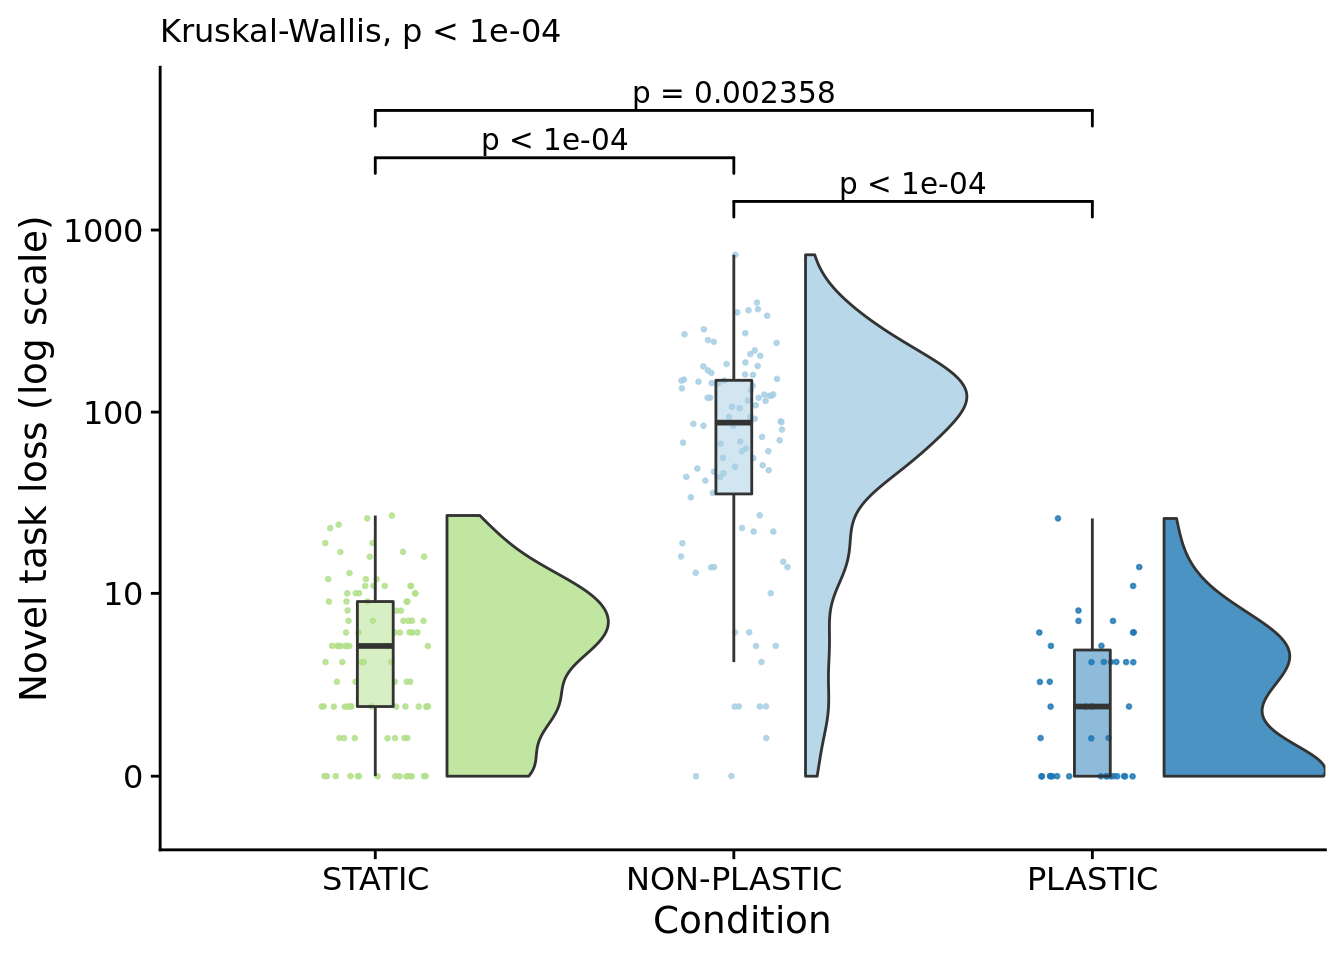
\includegraphics{supplemental-material_files/figure-latex/unnamed-chunk-59-1.pdf}

\begin{Shaded}
\begin{Highlighting}[]
\KeywordTok{paste0}\NormalTok{(}
  \StringTok{"PLASTIC median: "}\NormalTok{,}
  \KeywordTok{median}\NormalTok{(}\KeywordTok{filter}\NormalTok{(summary_data, condition}\OperatorTok{==}\StringTok{"PLASTIC"}\NormalTok{)}\OperatorTok{$}\NormalTok{discovered_extra_tasks_}\FloatTok{0.01}\NormalTok{)}
\NormalTok{)}
\end{Highlighting}
\end{Shaded}

\begin{verbatim}
## [1] "PLASTIC median: 8"
\end{verbatim}

\begin{Shaded}
\begin{Highlighting}[]
\KeywordTok{paste0}\NormalTok{(}
  \StringTok{"STATIC median: "}\NormalTok{,}
  \KeywordTok{median}\NormalTok{(}\KeywordTok{filter}\NormalTok{(summary_data, condition}\OperatorTok{==}\StringTok{"STATIC"}\NormalTok{)}\OperatorTok{$}\NormalTok{discovered_extra_tasks_}\FloatTok{0.01}\NormalTok{)}
\NormalTok{)}
\end{Highlighting}
\end{Shaded}

\begin{verbatim}
## [1] "STATIC median: 9"
\end{verbatim}

\begin{Shaded}
\begin{Highlighting}[]
\KeywordTok{paste0}\NormalTok{(}
  \StringTok{"NON-PLASTIC median: "}\NormalTok{,}
  \KeywordTok{median}\NormalTok{(}\KeywordTok{filter}\NormalTok{(summary_data, condition}\OperatorTok{==}\StringTok{"NON-PLASTIC"}\NormalTok{)}\OperatorTok{$}\NormalTok{discovered_extra_tasks_}\FloatTok{0.01}\NormalTok{)}
\NormalTok{)}
\end{Highlighting}
\end{Shaded}

\begin{verbatim}
## [1] "NON-PLASTIC median: 13"
\end{verbatim}

\begin{Shaded}
\begin{Highlighting}[]
\NormalTok{reward_level <-}\StringTok{ }\FloatTok{0.1}
\NormalTok{dom_task_data <-}\StringTok{ }\KeywordTok{filter}\NormalTok{(summary_data, extra_task_value}\OperatorTok{==}\NormalTok{reward_level)}
\KeywordTok{kruskal.test}\NormalTok{(}
  \DataTypeTok{formula=}\NormalTok{discovered_extra_tasks_}\FloatTok{0.01}\OperatorTok{~}\NormalTok{condition,}
  \DataTypeTok{data=}\NormalTok{dom_task_data}
\NormalTok{)}
\end{Highlighting}
\end{Shaded}

\begin{verbatim}
## 
##  Kruskal-Wallis rank sum test
## 
## data:  discovered_extra_tasks_0.01 by condition
## Kruskal-Wallis chi-squared = 24.271, df = 2, p-value = 5.365e-06
\end{verbatim}

\begin{Shaded}
\begin{Highlighting}[]
\KeywordTok{pairwise.wilcox.test}\NormalTok{(}
  \DataTypeTok{x=}\NormalTok{dom_task_data}\OperatorTok{$}\NormalTok{discovered_extra_tasks_}\FloatTok{0.01}\NormalTok{,}
  \DataTypeTok{g=}\NormalTok{dom_task_data}\OperatorTok{$}\NormalTok{condition,}
  \DataTypeTok{p.adjust.method=}\StringTok{"bonferroni"}\NormalTok{,}
  \DataTypeTok{conf.int=}\OtherTok{TRUE}\NormalTok{,}
  \DataTypeTok{conf.level=}\FloatTok{0.95}
\NormalTok{)}
\end{Highlighting}
\end{Shaded}

\begin{verbatim}
## 
##  Pairwise comparisons using Wilcoxon rank sum test with continuity correction 
## 
## data:  dom_task_data$discovered_extra_tasks_0.01 and dom_task_data$condition 
## 
##         NON-PLASTIC PLASTIC
## PLASTIC 2.4e-05     -      
## STATIC  0.00035     1.00000
## 
## P value adjustment method: bonferroni
\end{verbatim}

\hypertarget{novel-tasks-along-lineage-of-final-dominant-genotype}{%
\section{Novel tasks along lineage of final dominant genotype}\label{novel-tasks-along-lineage-of-final-dominant-genotype}}

\hypertarget{novel-tasks-discovered}{%
\subsection{Novel tasks discovered}\label{novel-tasks-discovered}}

\begin{Shaded}
\begin{Highlighting}[]
\KeywordTok{ggplot}\NormalTok{(summary_data, }\KeywordTok{aes}\NormalTok{(}\DataTypeTok{x=}\NormalTok{condition, }\DataTypeTok{y=}\NormalTok{dominant_lineage_extra_traits_discovered, }\DataTypeTok{fill=}\NormalTok{condition)) }\OperatorTok{+}
\StringTok{  }\KeywordTok{geom_flat_violin}\NormalTok{(}
    \DataTypeTok{position =} \KeywordTok{position_nudge}\NormalTok{(}\DataTypeTok{x =} \FloatTok{.2}\NormalTok{, }\DataTypeTok{y =} \DecValTok{0}\NormalTok{),}
    \DataTypeTok{alpha =} \FloatTok{.8}
\NormalTok{  ) }\OperatorTok{+}
\StringTok{  }\KeywordTok{geom_point}\NormalTok{(}
    \DataTypeTok{mapping=}\KeywordTok{aes}\NormalTok{(}\DataTypeTok{color=}\NormalTok{condition),}
    \DataTypeTok{position =} \KeywordTok{position_jitter}\NormalTok{(}\DataTypeTok{width =} \FloatTok{.15}\NormalTok{),}
    \DataTypeTok{size =} \FloatTok{.5}\NormalTok{,}
    \DataTypeTok{alpha =} \FloatTok{0.8}
\NormalTok{  ) }\OperatorTok{+}
\StringTok{  }\KeywordTok{geom_boxplot}\NormalTok{(}
    \DataTypeTok{width =} \FloatTok{.1}\NormalTok{,}
    \DataTypeTok{outlier.shape =} \OtherTok{NA}\NormalTok{,}
    \DataTypeTok{alpha =} \FloatTok{0.5}
\NormalTok{  ) }\OperatorTok{+}
\StringTok{  }\KeywordTok{scale_x_discrete}\NormalTok{(}
    \DataTypeTok{name=}\StringTok{"Condition"}\NormalTok{,}
    \DataTypeTok{limits=}\NormalTok{condition_order}
\NormalTok{  ) }\OperatorTok{+}
\StringTok{  }\KeywordTok{ylab}\NormalTok{(}\StringTok{"Extra tasks discovered along dominant lineage"}\NormalTok{) }\OperatorTok{+}
\StringTok{  }\KeywordTok{facet_wrap}\NormalTok{(}
    \OperatorTok{~}\NormalTok{extra_task_value,}
    \DataTypeTok{labeller=}\NormalTok{label_both}
\NormalTok{  ) }\OperatorTok{+}
\StringTok{  }\KeywordTok{theme}\NormalTok{(}
    \DataTypeTok{legend.position=}\StringTok{"none"}
\NormalTok{  ) }\OperatorTok{+}
\StringTok{  }\KeywordTok{ggsave}\NormalTok{(}
    \KeywordTok{paste0}\NormalTok{(working_directory, }\StringTok{"plots/dominant-lineage-extra-tasks-discovered.pdf"}\NormalTok{),}
    \DataTypeTok{width=}\DecValTok{15}\NormalTok{,}
    \DataTypeTok{height=}\DecValTok{10}
\NormalTok{  )}
\end{Highlighting}
\end{Shaded}

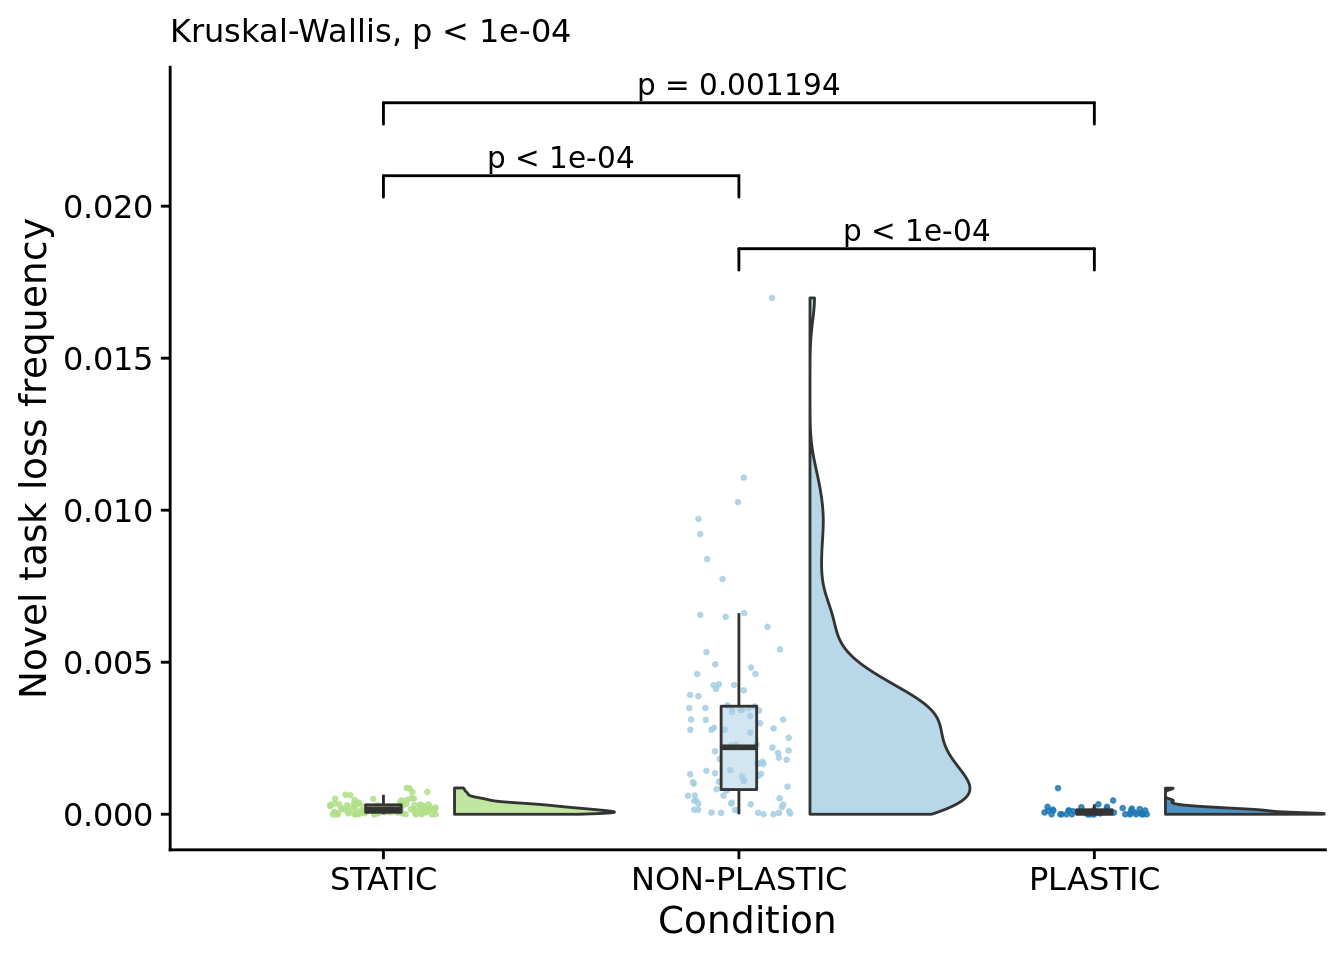
\includegraphics{supplemental-material_files/figure-latex/unnamed-chunk-61-1.pdf}

\begin{Shaded}
\begin{Highlighting}[]
\KeywordTok{paste0}\NormalTok{(}
  \StringTok{"PLASTIC median: "}\NormalTok{,}
  \KeywordTok{median}\NormalTok{(}\KeywordTok{filter}\NormalTok{(summary_data, condition}\OperatorTok{==}\StringTok{"PLASTIC"}\NormalTok{)}\OperatorTok{$}\NormalTok{dominant_lineage_extra_traits_discovered)}
\NormalTok{)}
\end{Highlighting}
\end{Shaded}

\begin{verbatim}
## [1] "PLASTIC median: 3.5"
\end{verbatim}

\begin{Shaded}
\begin{Highlighting}[]
\KeywordTok{paste0}\NormalTok{(}
  \StringTok{"STATIC median: "}\NormalTok{,}
  \KeywordTok{median}\NormalTok{(}\KeywordTok{filter}\NormalTok{(summary_data, condition}\OperatorTok{==}\StringTok{"STATIC"}\NormalTok{)}\OperatorTok{$}\NormalTok{dominant_lineage_extra_traits_discovered)}
\NormalTok{)}
\end{Highlighting}
\end{Shaded}

\begin{verbatim}
## [1] "STATIC median: 4"
\end{verbatim}

\begin{Shaded}
\begin{Highlighting}[]
\KeywordTok{paste0}\NormalTok{(}
  \StringTok{"NON-PLASTIC median: "}\NormalTok{,}
  \KeywordTok{median}\NormalTok{(}\KeywordTok{filter}\NormalTok{(summary_data, condition}\OperatorTok{==}\StringTok{"NON-PLASTIC"}\NormalTok{)}\OperatorTok{$}\NormalTok{dominant_lineage_extra_traits_discovered)}
\NormalTok{)}
\end{Highlighting}
\end{Shaded}

\begin{verbatim}
## [1] "NON-PLASTIC median: 6"
\end{verbatim}

\begin{Shaded}
\begin{Highlighting}[]
\NormalTok{reward_level <-}\StringTok{ }\FloatTok{0.1}
\NormalTok{dom_task_data <-}\StringTok{ }\KeywordTok{filter}\NormalTok{(summary_data, extra_task_value}\OperatorTok{==}\NormalTok{reward_level)}
\KeywordTok{kruskal.test}\NormalTok{(}
  \DataTypeTok{formula=}\NormalTok{dominant_lineage_extra_traits_discovered}\OperatorTok{~}\NormalTok{condition,}
  \DataTypeTok{data=}\NormalTok{dom_task_data}
\NormalTok{)}
\end{Highlighting}
\end{Shaded}

\begin{verbatim}
## 
##  Kruskal-Wallis rank sum test
## 
## data:  dominant_lineage_extra_traits_discovered by condition
## Kruskal-Wallis chi-squared = 24.099, df = 2, p-value = 5.846e-06
\end{verbatim}

\begin{Shaded}
\begin{Highlighting}[]
\KeywordTok{pairwise.wilcox.test}\NormalTok{(}
  \DataTypeTok{x=}\NormalTok{dom_task_data}\OperatorTok{$}\NormalTok{dominant_lineage_extra_traits_discovered,}
  \DataTypeTok{g=}\NormalTok{dom_task_data}\OperatorTok{$}\NormalTok{condition,}
  \DataTypeTok{p.adjust.method=}\StringTok{"bonferroni"}\NormalTok{,}
  \DataTypeTok{conf.int=}\OtherTok{TRUE}\NormalTok{,}
  \DataTypeTok{conf.level=}\FloatTok{0.95}
\NormalTok{)}
\end{Highlighting}
\end{Shaded}

\begin{verbatim}
## 
##  Pairwise comparisons using Wilcoxon rank sum test with continuity correction 
## 
## data:  dom_task_data$dominant_lineage_extra_traits_discovered and dom_task_data$condition 
## 
##         NON-PLASTIC PLASTIC
## PLASTIC 1.7e-05     -      
## STATIC  0.0035      0.0561 
## 
## P value adjustment method: bonferroni
\end{verbatim}

\hypertarget{novel-traits-discovered-per-step}{%
\subsubsection{Novel traits discovered per step}\label{novel-traits-discovered-per-step}}

This isn't totally fair to non-plastic lineages because they're continuously re-adapting, so they have
more genotypes along lineage.

\begin{Shaded}
\begin{Highlighting}[]
\NormalTok{summary_data}\OperatorTok{$}\NormalTok{dominant_lineage_extra_traits_discovered_per_step <-}\StringTok{ }\NormalTok{summary_data}\OperatorTok{$}\NormalTok{dominant_lineage_extra_traits_discovered }\OperatorTok{/}\StringTok{ }\NormalTok{summary_data}\OperatorTok{$}\NormalTok{dominant_lineage_length_genotypes}
\KeywordTok{ggplot}\NormalTok{(summary_data, }\KeywordTok{aes}\NormalTok{(}\DataTypeTok{x=}\NormalTok{condition, }\DataTypeTok{y=}\NormalTok{dominant_lineage_extra_traits_discovered_per_step, }\DataTypeTok{fill=}\NormalTok{condition)) }\OperatorTok{+}
\StringTok{  }\KeywordTok{geom_flat_violin}\NormalTok{(}
    \DataTypeTok{position =} \KeywordTok{position_nudge}\NormalTok{(}\DataTypeTok{x =} \FloatTok{.2}\NormalTok{, }\DataTypeTok{y =} \DecValTok{0}\NormalTok{),}
    \DataTypeTok{alpha =} \FloatTok{.8}
\NormalTok{  ) }\OperatorTok{+}
\StringTok{  }\KeywordTok{geom_point}\NormalTok{(}
    \DataTypeTok{mapping=}\KeywordTok{aes}\NormalTok{(}\DataTypeTok{color=}\NormalTok{condition),}
    \DataTypeTok{position =} \KeywordTok{position_jitter}\NormalTok{(}\DataTypeTok{width =} \FloatTok{.15}\NormalTok{),}
    \DataTypeTok{size =} \FloatTok{.5}\NormalTok{,}
    \DataTypeTok{alpha =} \FloatTok{0.8}
\NormalTok{  ) }\OperatorTok{+}
\StringTok{  }\KeywordTok{geom_boxplot}\NormalTok{(}
    \DataTypeTok{width =} \FloatTok{.1}\NormalTok{,}
    \DataTypeTok{outlier.shape =} \OtherTok{NA}\NormalTok{,}
    \DataTypeTok{alpha =} \FloatTok{0.5}
\NormalTok{  ) }\OperatorTok{+}
\StringTok{  }\KeywordTok{scale_x_discrete}\NormalTok{(}
    \DataTypeTok{name=}\StringTok{"Condition"}\NormalTok{,}
    \DataTypeTok{limits=}\NormalTok{condition_order}
\NormalTok{  ) }\OperatorTok{+}
\StringTok{  }\KeywordTok{ylab}\NormalTok{(}\StringTok{"Lineage task discovery (per step)"}\NormalTok{) }\OperatorTok{+}
\StringTok{  }\KeywordTok{facet_wrap}\NormalTok{(}
    \OperatorTok{~}\NormalTok{extra_task_value,}
    \DataTypeTok{labeller=}\NormalTok{label_both}
\NormalTok{  ) }\OperatorTok{+}
\StringTok{  }\KeywordTok{theme}\NormalTok{(}
    \DataTypeTok{legend.position=}\StringTok{"none"}
\NormalTok{  )}
\end{Highlighting}
\end{Shaded}

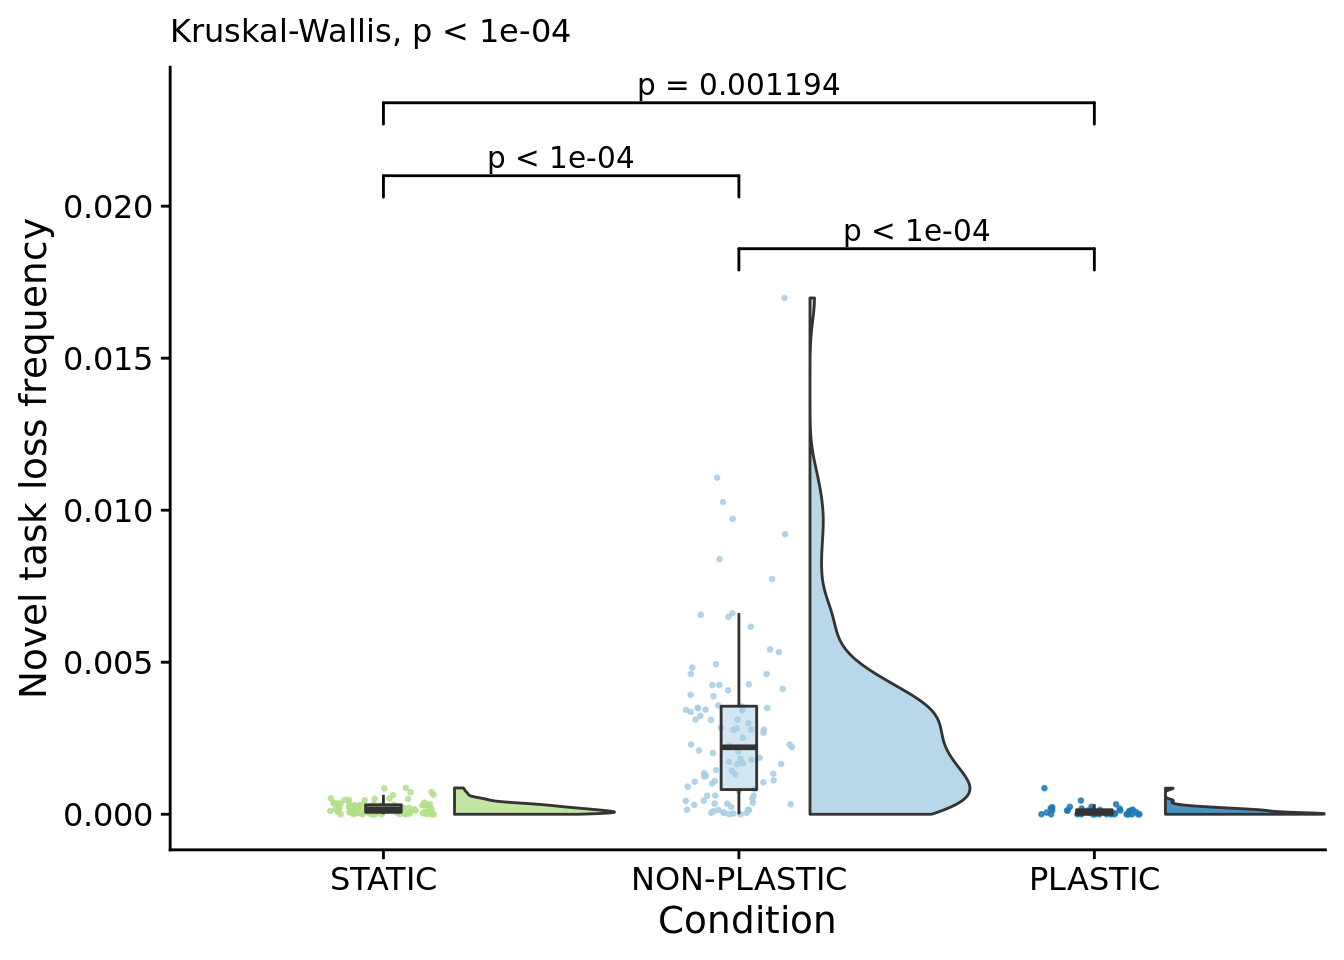
\includegraphics{supplemental-material_files/figure-latex/unnamed-chunk-63-1.pdf}

\begin{Shaded}
\begin{Highlighting}[]
\KeywordTok{paste0}\NormalTok{(}
  \StringTok{"PLASTIC median: "}\NormalTok{,}
  \KeywordTok{median}\NormalTok{(}\KeywordTok{filter}\NormalTok{(summary_data, condition}\OperatorTok{==}\StringTok{"PLASTIC"}\NormalTok{)}\OperatorTok{$}\NormalTok{dominant_lineage_extra_traits_discovered_per_step)}
\NormalTok{)}
\end{Highlighting}
\end{Shaded}

\begin{verbatim}
## [1] "PLASTIC median: 0.00484428434398198"
\end{verbatim}

\begin{Shaded}
\begin{Highlighting}[]
\KeywordTok{paste0}\NormalTok{(}
  \StringTok{"STATIC median: "}\NormalTok{,}
  \KeywordTok{median}\NormalTok{(}\KeywordTok{filter}\NormalTok{(summary_data, condition}\OperatorTok{==}\StringTok{"STATIC"}\NormalTok{)}\OperatorTok{$}\NormalTok{dominant_lineage_extra_traits_discovered_per_step)}
\NormalTok{)}
\end{Highlighting}
\end{Shaded}

\begin{verbatim}
## [1] "STATIC median: 0.00480194844967106"
\end{verbatim}

\begin{Shaded}
\begin{Highlighting}[]
\KeywordTok{paste0}\NormalTok{(}
  \StringTok{"NON-PLASTIC median: "}\NormalTok{,}
  \KeywordTok{median}\NormalTok{(}\KeywordTok{filter}\NormalTok{(summary_data, condition}\OperatorTok{==}\StringTok{"NON-PLASTIC"}\NormalTok{)}\OperatorTok{$}\NormalTok{dominant_lineage_extra_traits_discovered_per_step)}
\NormalTok{)}
\end{Highlighting}
\end{Shaded}

\begin{verbatim}
## [1] "NON-PLASTIC median: 0.00139827576402932"
\end{verbatim}

\begin{Shaded}
\begin{Highlighting}[]
\NormalTok{reward_level <-}\StringTok{ }\FloatTok{0.1}
\NormalTok{dom_task_data <-}\StringTok{ }\KeywordTok{filter}\NormalTok{(summary_data, extra_task_value}\OperatorTok{==}\NormalTok{reward_level)}
\KeywordTok{kruskal.test}\NormalTok{(}
  \DataTypeTok{formula=}\NormalTok{dominant_lineage_extra_traits_discovered_per_step}\OperatorTok{~}\NormalTok{condition,}
  \DataTypeTok{data=}\NormalTok{dom_task_data}
\NormalTok{)}
\end{Highlighting}
\end{Shaded}

\begin{verbatim}
## 
##  Kruskal-Wallis rank sum test
## 
## data:  dominant_lineage_extra_traits_discovered_per_step by condition
## Kruskal-Wallis chi-squared = 106.72, df = 2, p-value < 2.2e-16
\end{verbatim}

\begin{Shaded}
\begin{Highlighting}[]
\KeywordTok{pairwise.wilcox.test}\NormalTok{(}
  \DataTypeTok{x=}\NormalTok{dom_task_data}\OperatorTok{$}\NormalTok{dominant_lineage_extra_traits_discovered_per_step,}
  \DataTypeTok{g=}\NormalTok{dom_task_data}\OperatorTok{$}\NormalTok{condition,}
  \DataTypeTok{p.adjust.method=}\StringTok{"bonferroni"}\NormalTok{,}
  \DataTypeTok{conf.int=}\OtherTok{TRUE}\NormalTok{,}
  \DataTypeTok{conf.level=}\FloatTok{0.95}
\NormalTok{)}
\end{Highlighting}
\end{Shaded}

\begin{verbatim}
## 
##  Pairwise comparisons using Wilcoxon rank sum test with continuity correction 
## 
## data:  dom_task_data$dominant_lineage_extra_traits_discovered_per_step and dom_task_data$condition 
## 
##         NON-PLASTIC PLASTIC
## PLASTIC 9.7e-11     -      
## STATIC  < 2e-16     0.67   
## 
## P value adjustment method: bonferroni
\end{verbatim}

\hypertarget{novel-tasks-discovered-per-generation}{%
\subsection{Novel tasks discovered per generation}\label{novel-tasks-discovered-per-generation}}

\begin{Shaded}
\begin{Highlighting}[]
\NormalTok{summary_data}\OperatorTok{$}\NormalTok{dominant_lineage_extra_traits_discovered_per_generation <-}\StringTok{ }\NormalTok{summary_data}\OperatorTok{$}\NormalTok{dominant_lineage_extra_traits_discovered }\OperatorTok{/}\StringTok{ }\NormalTok{summary_data}\OperatorTok{$}\NormalTok{dominant_generation_born}
\KeywordTok{ggplot}\NormalTok{(summary_data, }\KeywordTok{aes}\NormalTok{(}\DataTypeTok{x=}\NormalTok{condition, }\DataTypeTok{y=}\NormalTok{dominant_lineage_extra_traits_discovered_per_generation, }\DataTypeTok{fill=}\NormalTok{condition)) }\OperatorTok{+}
\StringTok{  }\KeywordTok{geom_flat_violin}\NormalTok{(}
    \DataTypeTok{position =} \KeywordTok{position_nudge}\NormalTok{(}\DataTypeTok{x =} \FloatTok{.2}\NormalTok{, }\DataTypeTok{y =} \DecValTok{0}\NormalTok{),}
    \DataTypeTok{alpha =} \FloatTok{.8}
\NormalTok{  ) }\OperatorTok{+}
\StringTok{  }\KeywordTok{geom_point}\NormalTok{(}
    \DataTypeTok{mapping=}\KeywordTok{aes}\NormalTok{(}\DataTypeTok{color=}\NormalTok{condition),}
    \DataTypeTok{position =} \KeywordTok{position_jitter}\NormalTok{(}\DataTypeTok{width =} \FloatTok{.15}\NormalTok{),}
    \DataTypeTok{size =} \FloatTok{.5}\NormalTok{,}
    \DataTypeTok{alpha =} \FloatTok{0.8}
\NormalTok{  ) }\OperatorTok{+}
\StringTok{  }\KeywordTok{geom_boxplot}\NormalTok{(}
    \DataTypeTok{width =} \FloatTok{.1}\NormalTok{,}
    \DataTypeTok{outlier.shape =} \OtherTok{NA}\NormalTok{,}
    \DataTypeTok{alpha =} \FloatTok{0.5}
\NormalTok{  ) }\OperatorTok{+}
\StringTok{  }\KeywordTok{scale_x_discrete}\NormalTok{(}
    \DataTypeTok{name=}\StringTok{"Condition"}\NormalTok{,}
    \DataTypeTok{limits=}\NormalTok{condition_order}
\NormalTok{  ) }\OperatorTok{+}
\StringTok{  }\KeywordTok{ylab}\NormalTok{(}\StringTok{"Lineage task discovery (per generation)"}\NormalTok{) }\OperatorTok{+}
\StringTok{  }\KeywordTok{facet_wrap}\NormalTok{(}
    \OperatorTok{~}\NormalTok{extra_task_value,}
    \DataTypeTok{labeller=}\NormalTok{label_both}
\NormalTok{  ) }\OperatorTok{+}
\StringTok{  }\KeywordTok{theme}\NormalTok{(}
    \DataTypeTok{legend.position=}\StringTok{"none"}
\NormalTok{  )}
\end{Highlighting}
\end{Shaded}

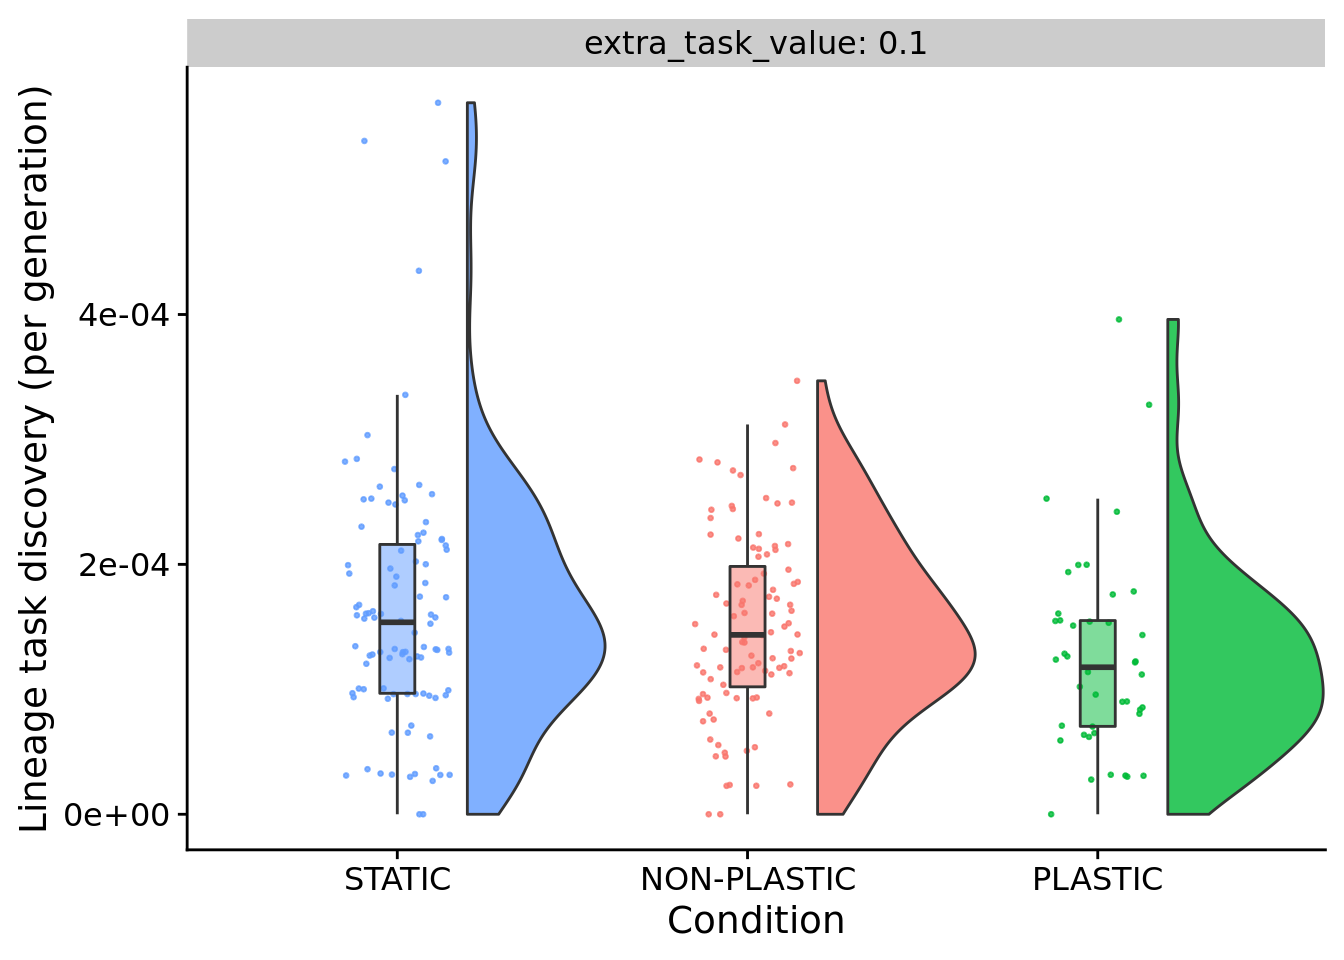
\includegraphics{supplemental-material_files/figure-latex/unnamed-chunk-65-1.pdf}

\begin{Shaded}
\begin{Highlighting}[]
\KeywordTok{paste0}\NormalTok{(}
  \StringTok{"PLASTIC median: "}\NormalTok{,}
  \KeywordTok{median}\NormalTok{(}\KeywordTok{filter}\NormalTok{(summary_data, condition}\OperatorTok{==}\StringTok{"PLASTIC"}\NormalTok{)}\OperatorTok{$}\NormalTok{dominant_lineage_extra_traits_discovered_per_generation)}
\NormalTok{)}
\end{Highlighting}
\end{Shaded}

\begin{verbatim}
## [1] "PLASTIC median: 0.000117695011124939"
\end{verbatim}

\begin{Shaded}
\begin{Highlighting}[]
\KeywordTok{paste0}\NormalTok{(}
  \StringTok{"STATIC median: "}\NormalTok{,}
  \KeywordTok{median}\NormalTok{(}\KeywordTok{filter}\NormalTok{(summary_data, condition}\OperatorTok{==}\StringTok{"STATIC"}\NormalTok{)}\OperatorTok{$}\NormalTok{dominant_lineage_extra_traits_discovered_per_generation)}
\NormalTok{)}
\end{Highlighting}
\end{Shaded}

\begin{verbatim}
## [1] "STATIC median: 0.00015363220504867"
\end{verbatim}

\begin{Shaded}
\begin{Highlighting}[]
\KeywordTok{paste0}\NormalTok{(}
  \StringTok{"NON-PLASTIC median: "}\NormalTok{,}
  \KeywordTok{median}\NormalTok{(}\KeywordTok{filter}\NormalTok{(summary_data, condition}\OperatorTok{==}\StringTok{"NON-PLASTIC"}\NormalTok{)}\OperatorTok{$}\NormalTok{dominant_lineage_extra_traits_discovered_per_generation)}
\NormalTok{)}
\end{Highlighting}
\end{Shaded}

\begin{verbatim}
## [1] "NON-PLASTIC median: 0.00014358046266055"
\end{verbatim}

\begin{Shaded}
\begin{Highlighting}[]
\NormalTok{reward_level <-}\StringTok{ }\FloatTok{0.1}
\NormalTok{dom_task_data <-}\StringTok{ }\KeywordTok{filter}\NormalTok{(summary_data, extra_task_value}\OperatorTok{==}\NormalTok{reward_level)}
\KeywordTok{kruskal.test}\NormalTok{(}
  \DataTypeTok{formula=}\NormalTok{dominant_lineage_extra_traits_discovered_per_generation}\OperatorTok{~}\NormalTok{condition,}
  \DataTypeTok{data=}\NormalTok{dom_task_data}
\NormalTok{)}
\end{Highlighting}
\end{Shaded}

\begin{verbatim}
## 
##  Kruskal-Wallis rank sum test
## 
## data:  dominant_lineage_extra_traits_discovered_per_generation by condition
## Kruskal-Wallis chi-squared = 7.1465, df = 2, p-value = 0.02806
\end{verbatim}

\begin{Shaded}
\begin{Highlighting}[]
\KeywordTok{pairwise.wilcox.test}\NormalTok{(}
  \DataTypeTok{x=}\NormalTok{dom_task_data}\OperatorTok{$}\NormalTok{dominant_lineage_extra_traits_discovered_per_generation,}
  \DataTypeTok{g=}\NormalTok{dom_task_data}\OperatorTok{$}\NormalTok{condition,}
  \DataTypeTok{p.adjust.method=}\StringTok{"bonferroni"}\NormalTok{,}
  \DataTypeTok{conf.int=}\OtherTok{TRUE}\NormalTok{,}
  \DataTypeTok{conf.level=}\FloatTok{0.95}
\NormalTok{)}
\end{Highlighting}
\end{Shaded}

\begin{verbatim}
## 
##  Pairwise comparisons using Wilcoxon rank sum test with continuity correction 
## 
## data:  dom_task_data$dominant_lineage_extra_traits_discovered_per_generation and dom_task_data$condition 
## 
##         NON-PLASTIC PLASTIC
## PLASTIC 0.092       -      
## STATIC  1.000       0.025  
## 
## P value adjustment method: bonferroni
\end{verbatim}

\hypertarget{novel-tasks-gained}{%
\subsection{Novel tasks gained}\label{novel-tasks-gained}}

\begin{Shaded}
\begin{Highlighting}[]
\KeywordTok{ggplot}\NormalTok{(summary_data, }\KeywordTok{aes}\NormalTok{(}\DataTypeTok{x=}\NormalTok{condition, }\DataTypeTok{y=}\NormalTok{dominant_lineage_extra_traits_gained, }\DataTypeTok{fill=}\NormalTok{condition)) }\OperatorTok{+}
\StringTok{  }\KeywordTok{geom_flat_violin}\NormalTok{(}
    \DataTypeTok{position =} \KeywordTok{position_nudge}\NormalTok{(}\DataTypeTok{x =} \FloatTok{.2}\NormalTok{, }\DataTypeTok{y =} \DecValTok{0}\NormalTok{),}
    \DataTypeTok{alpha =} \FloatTok{.8}
\NormalTok{  ) }\OperatorTok{+}
\StringTok{  }\KeywordTok{geom_point}\NormalTok{(}
    \DataTypeTok{mapping=}\KeywordTok{aes}\NormalTok{(}\DataTypeTok{color=}\NormalTok{condition),}
    \DataTypeTok{position =} \KeywordTok{position_jitter}\NormalTok{(}\DataTypeTok{width =} \FloatTok{.15}\NormalTok{),}
    \DataTypeTok{size =} \FloatTok{.5}\NormalTok{,}
    \DataTypeTok{alpha =} \FloatTok{0.8}
\NormalTok{  ) }\OperatorTok{+}
\StringTok{  }\KeywordTok{geom_boxplot}\NormalTok{(}
    \DataTypeTok{width =} \FloatTok{.1}\NormalTok{,}
    \DataTypeTok{outlier.shape =} \OtherTok{NA}\NormalTok{,}
    \DataTypeTok{alpha =} \FloatTok{0.5}
\NormalTok{  ) }\OperatorTok{+}
\StringTok{  }\KeywordTok{scale_x_discrete}\NormalTok{(}
    \DataTypeTok{name=}\StringTok{"Condition"}\NormalTok{,}
    \DataTypeTok{limits=}\NormalTok{condition_order}
\NormalTok{  ) }\OperatorTok{+}
\StringTok{  }\KeywordTok{ylab}\NormalTok{(}\StringTok{"Extra tasks gained along dominant lineage"}\NormalTok{) }\OperatorTok{+}
\StringTok{  }\KeywordTok{facet_wrap}\NormalTok{(}
    \OperatorTok{~}\NormalTok{extra_task_value,}
    \DataTypeTok{labeller=}\NormalTok{label_both}
\NormalTok{  ) }\OperatorTok{+}
\StringTok{  }\KeywordTok{theme}\NormalTok{(}
    \DataTypeTok{legend.position=}\StringTok{"none"}
\NormalTok{  ) }\OperatorTok{+}
\StringTok{  }\KeywordTok{ggsave}\NormalTok{(}
    \KeywordTok{paste0}\NormalTok{(working_directory, }\StringTok{"plots/dominant-lineage-extra-tasks-gained.pdf"}\NormalTok{),}
    \DataTypeTok{width=}\DecValTok{15}\NormalTok{,}
    \DataTypeTok{height=}\DecValTok{10}
\NormalTok{  )}
\end{Highlighting}
\end{Shaded}

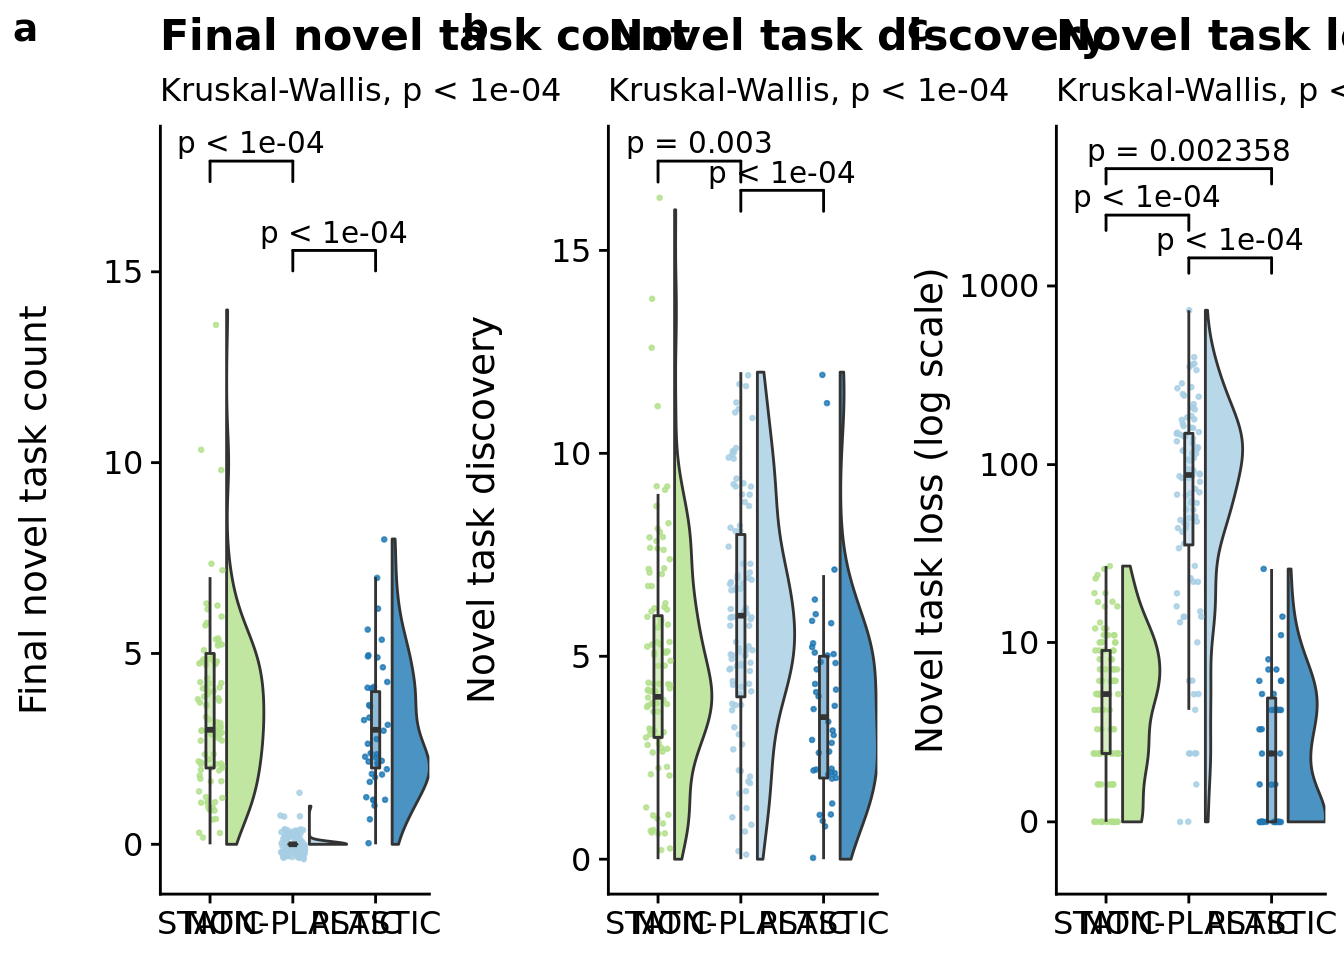
\includegraphics{supplemental-material_files/figure-latex/unnamed-chunk-67-1.pdf}

\hypertarget{novel-tasks-lost}{%
\subsection{Novel tasks lost}\label{novel-tasks-lost}}

\begin{Shaded}
\begin{Highlighting}[]
\KeywordTok{ggplot}\NormalTok{(summary_data, }\KeywordTok{aes}\NormalTok{(}\DataTypeTok{x=}\NormalTok{condition, }\DataTypeTok{y=}\NormalTok{dominant_lineage_extra_traits_lost, }\DataTypeTok{fill=}\NormalTok{condition)) }\OperatorTok{+}
\StringTok{  }\KeywordTok{geom_flat_violin}\NormalTok{(}
    \DataTypeTok{position =} \KeywordTok{position_nudge}\NormalTok{(}\DataTypeTok{x =} \FloatTok{.2}\NormalTok{, }\DataTypeTok{y =} \DecValTok{0}\NormalTok{),}
    \DataTypeTok{alpha =} \FloatTok{.8}
\NormalTok{  ) }\OperatorTok{+}
\StringTok{  }\KeywordTok{geom_point}\NormalTok{(}
    \DataTypeTok{mapping=}\KeywordTok{aes}\NormalTok{(}\DataTypeTok{color=}\NormalTok{condition),}
    \DataTypeTok{position =} \KeywordTok{position_jitter}\NormalTok{(}\DataTypeTok{width =} \FloatTok{.15}\NormalTok{),}
    \DataTypeTok{size =} \FloatTok{.5}\NormalTok{,}
    \DataTypeTok{alpha =} \FloatTok{0.8}
\NormalTok{  ) }\OperatorTok{+}
\StringTok{  }\KeywordTok{geom_boxplot}\NormalTok{(}
    \DataTypeTok{width =} \FloatTok{.1}\NormalTok{,}
    \DataTypeTok{outlier.shape =} \OtherTok{NA}\NormalTok{,}
    \DataTypeTok{alpha =} \FloatTok{0.5}
\NormalTok{  ) }\OperatorTok{+}
\StringTok{  }\KeywordTok{scale_x_discrete}\NormalTok{(}
    \DataTypeTok{name=}\StringTok{"Condition"}\NormalTok{,}
    \DataTypeTok{limits=}\NormalTok{condition_order}
\NormalTok{  ) }\OperatorTok{+}
\StringTok{  }\KeywordTok{ylab}\NormalTok{(}\StringTok{"Extra tasks lost along dominant lineage"}\NormalTok{) }\OperatorTok{+}
\StringTok{  }\KeywordTok{facet_wrap}\NormalTok{(}
    \OperatorTok{~}\NormalTok{extra_task_value,}
    \DataTypeTok{labeller=}\NormalTok{label_both}
\NormalTok{  ) }\OperatorTok{+}
\StringTok{  }\KeywordTok{theme}\NormalTok{(}
    \DataTypeTok{legend.position=}\StringTok{"none"}
\NormalTok{  ) }\OperatorTok{+}
\StringTok{  }\KeywordTok{ggsave}\NormalTok{(}
    \KeywordTok{paste0}\NormalTok{(working_directory, }\StringTok{"plots/dominant-lineage-extra-tasks-lost.pdf"}\NormalTok{),}
    \DataTypeTok{width=}\DecValTok{15}\NormalTok{,}
    \DataTypeTok{height=}\DecValTok{10}
\NormalTok{  )}
\end{Highlighting}
\end{Shaded}

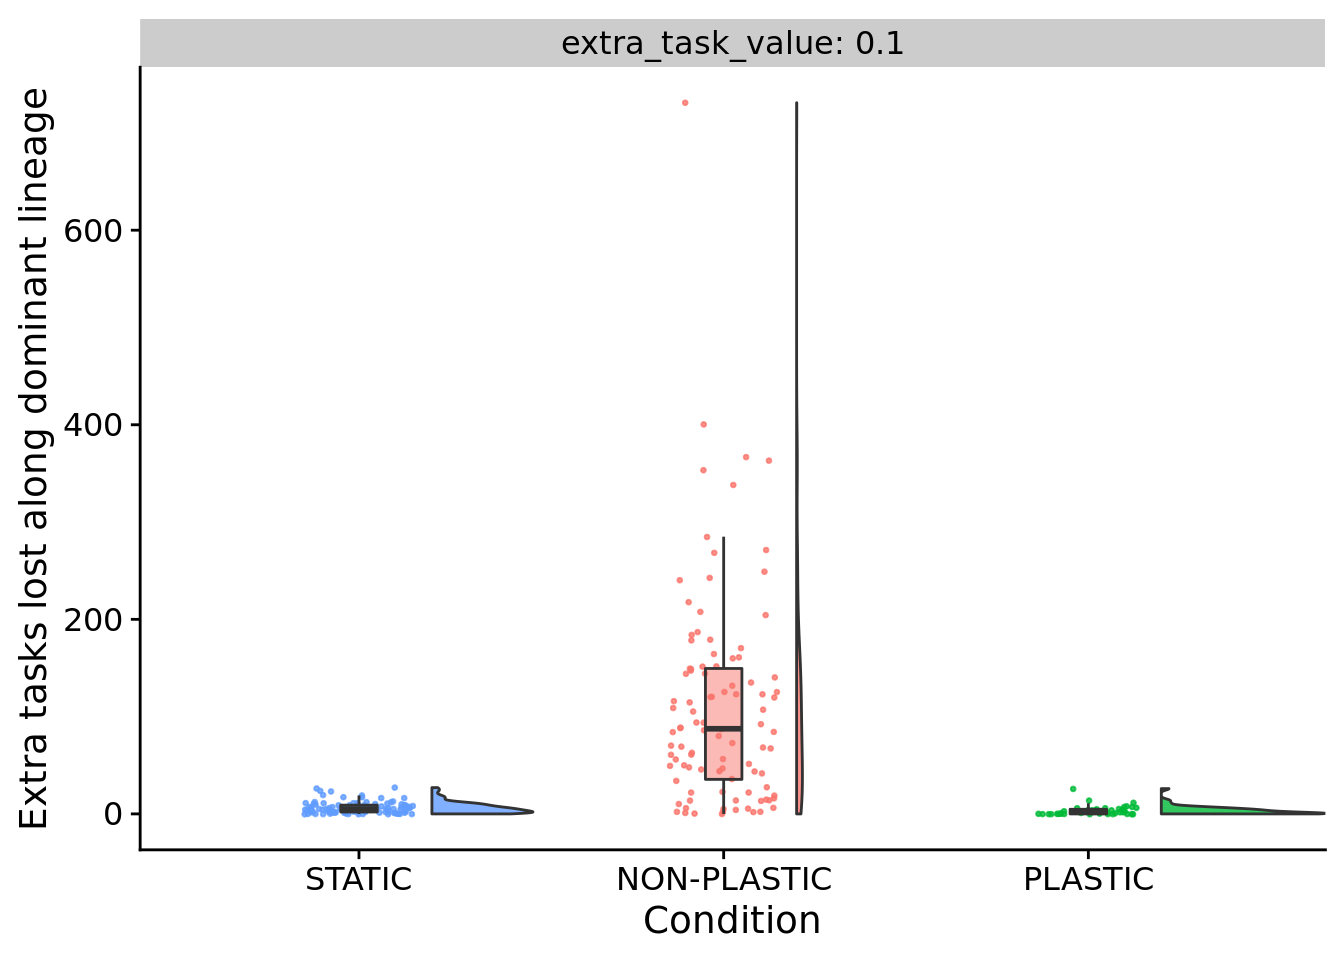
\includegraphics{supplemental-material_files/figure-latex/unnamed-chunk-68-1.pdf}

\begin{Shaded}
\begin{Highlighting}[]
\KeywordTok{paste0}\NormalTok{(}
  \StringTok{"PLASTIC median: "}\NormalTok{,}
  \KeywordTok{median}\NormalTok{(}\KeywordTok{filter}\NormalTok{(summary_data, condition}\OperatorTok{==}\StringTok{"PLASTIC"}\NormalTok{)}\OperatorTok{$}\NormalTok{dominant_lineage_extra_traits_lost)}
\NormalTok{)}
\end{Highlighting}
\end{Shaded}

\begin{verbatim}
## [1] "PLASTIC median: 2"
\end{verbatim}

\begin{Shaded}
\begin{Highlighting}[]
\KeywordTok{paste0}\NormalTok{(}
  \StringTok{"STATIC median: "}\NormalTok{,}
  \KeywordTok{median}\NormalTok{(}\KeywordTok{filter}\NormalTok{(summary_data, condition}\OperatorTok{==}\StringTok{"STATIC"}\NormalTok{)}\OperatorTok{$}\NormalTok{dominant_lineage_extra_traits_lost)}
\NormalTok{)}
\end{Highlighting}
\end{Shaded}

\begin{verbatim}
## [1] "STATIC median: 5"
\end{verbatim}

\begin{Shaded}
\begin{Highlighting}[]
\KeywordTok{paste0}\NormalTok{(}
  \StringTok{"NON-PLASTIC median: "}\NormalTok{,}
  \KeywordTok{median}\NormalTok{(}\KeywordTok{filter}\NormalTok{(summary_data, condition}\OperatorTok{==}\StringTok{"NON-PLASTIC"}\NormalTok{)}\OperatorTok{$}\NormalTok{dominant_lineage_extra_traits_lost)}
\NormalTok{)}
\end{Highlighting}
\end{Shaded}

\begin{verbatim}
## [1] "NON-PLASTIC median: 87.5"
\end{verbatim}

\begin{Shaded}
\begin{Highlighting}[]
\NormalTok{reward_level <-}\StringTok{ }\FloatTok{0.1}
\NormalTok{dom_task_data <-}\StringTok{ }\KeywordTok{filter}\NormalTok{(summary_data, extra_task_value}\OperatorTok{==}\NormalTok{reward_level)}
\KeywordTok{kruskal.test}\NormalTok{(}
  \DataTypeTok{formula=}\NormalTok{dominant_lineage_extra_traits_lost}\OperatorTok{~}\NormalTok{condition,}
  \DataTypeTok{data=}\NormalTok{dom_task_data}
\NormalTok{)}
\end{Highlighting}
\end{Shaded}

\begin{verbatim}
## 
##  Kruskal-Wallis rank sum test
## 
## data:  dominant_lineage_extra_traits_lost by condition
## Kruskal-Wallis chi-squared = 129.06, df = 2, p-value < 2.2e-16
\end{verbatim}

\begin{Shaded}
\begin{Highlighting}[]
\KeywordTok{pairwise.wilcox.test}\NormalTok{(}
  \DataTypeTok{x=}\NormalTok{dom_task_data}\OperatorTok{$}\NormalTok{dominant_lineage_extra_traits_lost,}
  \DataTypeTok{g=}\NormalTok{dom_task_data}\OperatorTok{$}\NormalTok{condition,}
  \DataTypeTok{p.adjust.method=}\StringTok{"bonferroni"}\NormalTok{,}
  \DataTypeTok{conf.int=}\OtherTok{TRUE}\NormalTok{,}
  \DataTypeTok{conf.level=}\FloatTok{0.95}
\NormalTok{)}
\end{Highlighting}
\end{Shaded}

\begin{verbatim}
## 
##  Pairwise comparisons using Wilcoxon rank sum test with continuity correction 
## 
## data:  dom_task_data$dominant_lineage_extra_traits_lost and dom_task_data$condition 
## 
##         NON-PLASTIC PLASTIC
## PLASTIC 2.7e-16     -      
## STATIC  < 2e-16     0.0024 
## 
## P value adjustment method: bonferroni
\end{verbatim}

\hypertarget{novel-traits-lost-per-step}{%
\subsubsection{Novel traits lost per step}\label{novel-traits-lost-per-step}}

Again, not totally fair to non-plastic lineages.

\begin{Shaded}
\begin{Highlighting}[]
\NormalTok{summary_data}\OperatorTok{$}\NormalTok{dominant_lineage_extra_traits_lost_per_step <-}\StringTok{ }\NormalTok{summary_data}\OperatorTok{$}\NormalTok{dominant_lineage_extra_traits_lost }\OperatorTok{/}\StringTok{ }\NormalTok{summary_data}\OperatorTok{$}\NormalTok{dominant_lineage_length_genotypes}
\KeywordTok{ggplot}\NormalTok{(summary_data, }\KeywordTok{aes}\NormalTok{(}\DataTypeTok{x=}\NormalTok{condition, }\DataTypeTok{y=}\NormalTok{dominant_lineage_extra_traits_lost_per_step, }\DataTypeTok{fill=}\NormalTok{condition)) }\OperatorTok{+}
\StringTok{  }\KeywordTok{geom_flat_violin}\NormalTok{(}
    \DataTypeTok{position =} \KeywordTok{position_nudge}\NormalTok{(}\DataTypeTok{x =} \FloatTok{.2}\NormalTok{, }\DataTypeTok{y =} \DecValTok{0}\NormalTok{),}
    \DataTypeTok{alpha =} \FloatTok{.8}
\NormalTok{  ) }\OperatorTok{+}
\StringTok{  }\KeywordTok{geom_point}\NormalTok{(}
    \DataTypeTok{mapping=}\KeywordTok{aes}\NormalTok{(}\DataTypeTok{color=}\NormalTok{condition),}
    \DataTypeTok{position =} \KeywordTok{position_jitter}\NormalTok{(}\DataTypeTok{width =} \FloatTok{.15}\NormalTok{),}
    \DataTypeTok{size =} \FloatTok{.5}\NormalTok{,}
    \DataTypeTok{alpha =} \FloatTok{0.8}
\NormalTok{  ) }\OperatorTok{+}
\StringTok{  }\KeywordTok{geom_boxplot}\NormalTok{(}
    \DataTypeTok{width =} \FloatTok{.1}\NormalTok{,}
    \DataTypeTok{outlier.shape =} \OtherTok{NA}\NormalTok{,}
    \DataTypeTok{alpha =} \FloatTok{0.5}
\NormalTok{  ) }\OperatorTok{+}
\StringTok{  }\KeywordTok{scale_x_discrete}\NormalTok{(}
    \DataTypeTok{name=}\StringTok{"Condition"}\NormalTok{,}
    \DataTypeTok{limits=}\NormalTok{condition_order}
\NormalTok{  ) }\OperatorTok{+}
\StringTok{  }\KeywordTok{ylab}\NormalTok{(}\StringTok{"Extra tasks lost along dominant lineage (per step)"}\NormalTok{) }\OperatorTok{+}
\StringTok{  }\KeywordTok{facet_wrap}\NormalTok{(}
    \OperatorTok{~}\NormalTok{extra_task_value,}
    \DataTypeTok{labeller=}\NormalTok{label_both}
\NormalTok{  ) }\OperatorTok{+}
\StringTok{  }\KeywordTok{theme}\NormalTok{(}
    \DataTypeTok{legend.position=}\StringTok{"none"}
\NormalTok{  )}
\end{Highlighting}
\end{Shaded}

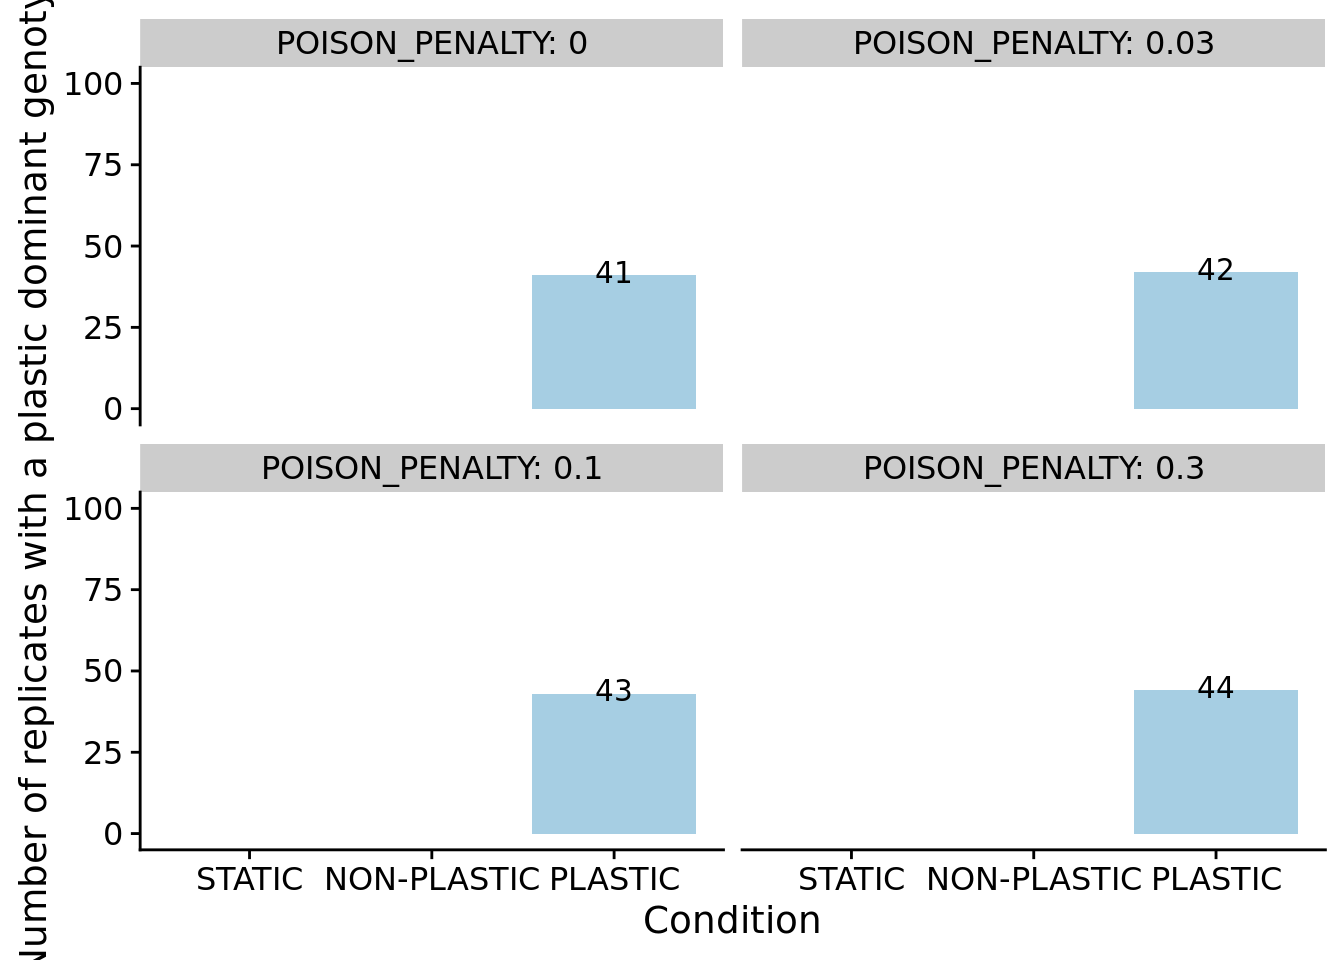
\includegraphics{supplemental-material_files/figure-latex/unnamed-chunk-70-1.pdf}

\begin{Shaded}
\begin{Highlighting}[]
\KeywordTok{paste0}\NormalTok{(}
  \StringTok{"PLASTIC median: "}\NormalTok{,}
  \KeywordTok{median}\NormalTok{(}\KeywordTok{filter}\NormalTok{(summary_data, condition}\OperatorTok{==}\StringTok{"PLASTIC"}\NormalTok{)}\OperatorTok{$}\NormalTok{dominant_lineage_extra_traits_lost_per_step)}
\NormalTok{)}
\end{Highlighting}
\end{Shaded}

\begin{verbatim}
## [1] "PLASTIC median: 0.00238455242036334"
\end{verbatim}

\begin{Shaded}
\begin{Highlighting}[]
\KeywordTok{paste0}\NormalTok{(}
  \StringTok{"STATIC median: "}\NormalTok{,}
  \KeywordTok{median}\NormalTok{(}\KeywordTok{filter}\NormalTok{(summary_data, condition}\OperatorTok{==}\StringTok{"STATIC"}\NormalTok{)}\OperatorTok{$}\NormalTok{dominant_lineage_extra_traits_lost_per_step)}
\NormalTok{)}
\end{Highlighting}
\end{Shaded}

\begin{verbatim}
## [1] "STATIC median: 0.00544747485837901"
\end{verbatim}

\begin{Shaded}
\begin{Highlighting}[]
\KeywordTok{paste0}\NormalTok{(}
  \StringTok{"NON-PLASTIC median: "}\NormalTok{,}
  \KeywordTok{median}\NormalTok{(}\KeywordTok{filter}\NormalTok{(summary_data, condition}\OperatorTok{==}\StringTok{"NON-PLASTIC"}\NormalTok{)}\OperatorTok{$}\NormalTok{dominant_lineage_extra_traits_lost_per_step)}
\NormalTok{)}
\end{Highlighting}
\end{Shaded}

\begin{verbatim}
## [1] "NON-PLASTIC median: 0.0216427755153431"
\end{verbatim}

\begin{Shaded}
\begin{Highlighting}[]
\NormalTok{reward_level <-}\StringTok{ }\FloatTok{0.1}
\NormalTok{dom_task_data <-}\StringTok{ }\KeywordTok{filter}\NormalTok{(summary_data, extra_task_value}\OperatorTok{==}\NormalTok{reward_level)}
\KeywordTok{kruskal.test}\NormalTok{(}
  \DataTypeTok{formula=}\NormalTok{dominant_lineage_extra_traits_lost_per_step}\OperatorTok{~}\NormalTok{condition,}
  \DataTypeTok{data=}\NormalTok{dom_task_data}
\NormalTok{)}
\end{Highlighting}
\end{Shaded}

\begin{verbatim}
## 
##  Kruskal-Wallis rank sum test
## 
## data:  dominant_lineage_extra_traits_lost_per_step by condition
## Kruskal-Wallis chi-squared = 65.779, df = 2, p-value = 5.204e-15
\end{verbatim}

\begin{Shaded}
\begin{Highlighting}[]
\KeywordTok{pairwise.wilcox.test}\NormalTok{(}
  \DataTypeTok{x=}\NormalTok{dom_task_data}\OperatorTok{$}\NormalTok{dominant_lineage_extra_traits_lost_per_step,}
  \DataTypeTok{g=}\NormalTok{dom_task_data}\OperatorTok{$}\NormalTok{condition,}
  \DataTypeTok{p.adjust.method=}\StringTok{"bonferroni"}\NormalTok{,}
  \DataTypeTok{conf.int=}\OtherTok{TRUE}\NormalTok{,}
  \DataTypeTok{conf.level=}\FloatTok{0.95}
\NormalTok{)}
\end{Highlighting}
\end{Shaded}

\begin{verbatim}
## 
##  Pairwise comparisons using Wilcoxon rank sum test with continuity correction 
## 
## data:  dom_task_data$dominant_lineage_extra_traits_lost_per_step and dom_task_data$condition 
## 
##         NON-PLASTIC PLASTIC
## PLASTIC 1.3e-10     -      
## STATIC  1.7e-10     0.0092 
## 
## P value adjustment method: bonferroni
\end{verbatim}

\hypertarget{novel-traits-lost-per-generation}{%
\subsubsection{Novel traits lost per generation}\label{novel-traits-lost-per-generation}}

\begin{Shaded}
\begin{Highlighting}[]
\NormalTok{summary_data}\OperatorTok{$}\NormalTok{dominant_lineage_extra_traits_lost_per_generation <-}\StringTok{ }\NormalTok{summary_data}\OperatorTok{$}\NormalTok{dominant_lineage_extra_traits_lost }\OperatorTok{/}\StringTok{ }\NormalTok{summary_data}\OperatorTok{$}\NormalTok{dominant_generation_born}
\KeywordTok{ggplot}\NormalTok{(summary_data, }\KeywordTok{aes}\NormalTok{(}\DataTypeTok{x=}\NormalTok{condition, }\DataTypeTok{y=}\NormalTok{dominant_lineage_extra_traits_lost_per_generation, }\DataTypeTok{fill=}\NormalTok{condition)) }\OperatorTok{+}
\StringTok{  }\KeywordTok{geom_flat_violin}\NormalTok{(}
    \DataTypeTok{position =} \KeywordTok{position_nudge}\NormalTok{(}\DataTypeTok{x =} \FloatTok{.2}\NormalTok{, }\DataTypeTok{y =} \DecValTok{0}\NormalTok{),}
    \DataTypeTok{alpha =} \FloatTok{.8}
\NormalTok{  ) }\OperatorTok{+}
\StringTok{  }\KeywordTok{geom_point}\NormalTok{(}
    \DataTypeTok{mapping=}\KeywordTok{aes}\NormalTok{(}\DataTypeTok{color=}\NormalTok{condition),}
    \DataTypeTok{position =} \KeywordTok{position_jitter}\NormalTok{(}\DataTypeTok{width =} \FloatTok{.15}\NormalTok{),}
    \DataTypeTok{size =} \FloatTok{.5}\NormalTok{,}
    \DataTypeTok{alpha =} \FloatTok{0.8}
\NormalTok{  ) }\OperatorTok{+}
\StringTok{  }\KeywordTok{geom_boxplot}\NormalTok{(}
    \DataTypeTok{width =} \FloatTok{.1}\NormalTok{,}
    \DataTypeTok{outlier.shape =} \OtherTok{NA}\NormalTok{,}
    \DataTypeTok{alpha =} \FloatTok{0.5}
\NormalTok{  ) }\OperatorTok{+}
\StringTok{  }\KeywordTok{scale_x_discrete}\NormalTok{(}
    \DataTypeTok{name=}\StringTok{"Condition"}\NormalTok{,}
    \DataTypeTok{limits=}\NormalTok{condition_order}
\NormalTok{  ) }\OperatorTok{+}
\StringTok{  }\KeywordTok{ylab}\NormalTok{(}\StringTok{"Extra tasks lost along dominant lineage (per generation)"}\NormalTok{) }\OperatorTok{+}
\StringTok{  }\KeywordTok{facet_wrap}\NormalTok{(}
    \OperatorTok{~}\NormalTok{extra_task_value,}
    \DataTypeTok{labeller=}\NormalTok{label_both}
\NormalTok{  ) }\OperatorTok{+}
\StringTok{  }\KeywordTok{theme}\NormalTok{(}
    \DataTypeTok{legend.position=}\StringTok{"none"}
\NormalTok{  )}
\end{Highlighting}
\end{Shaded}

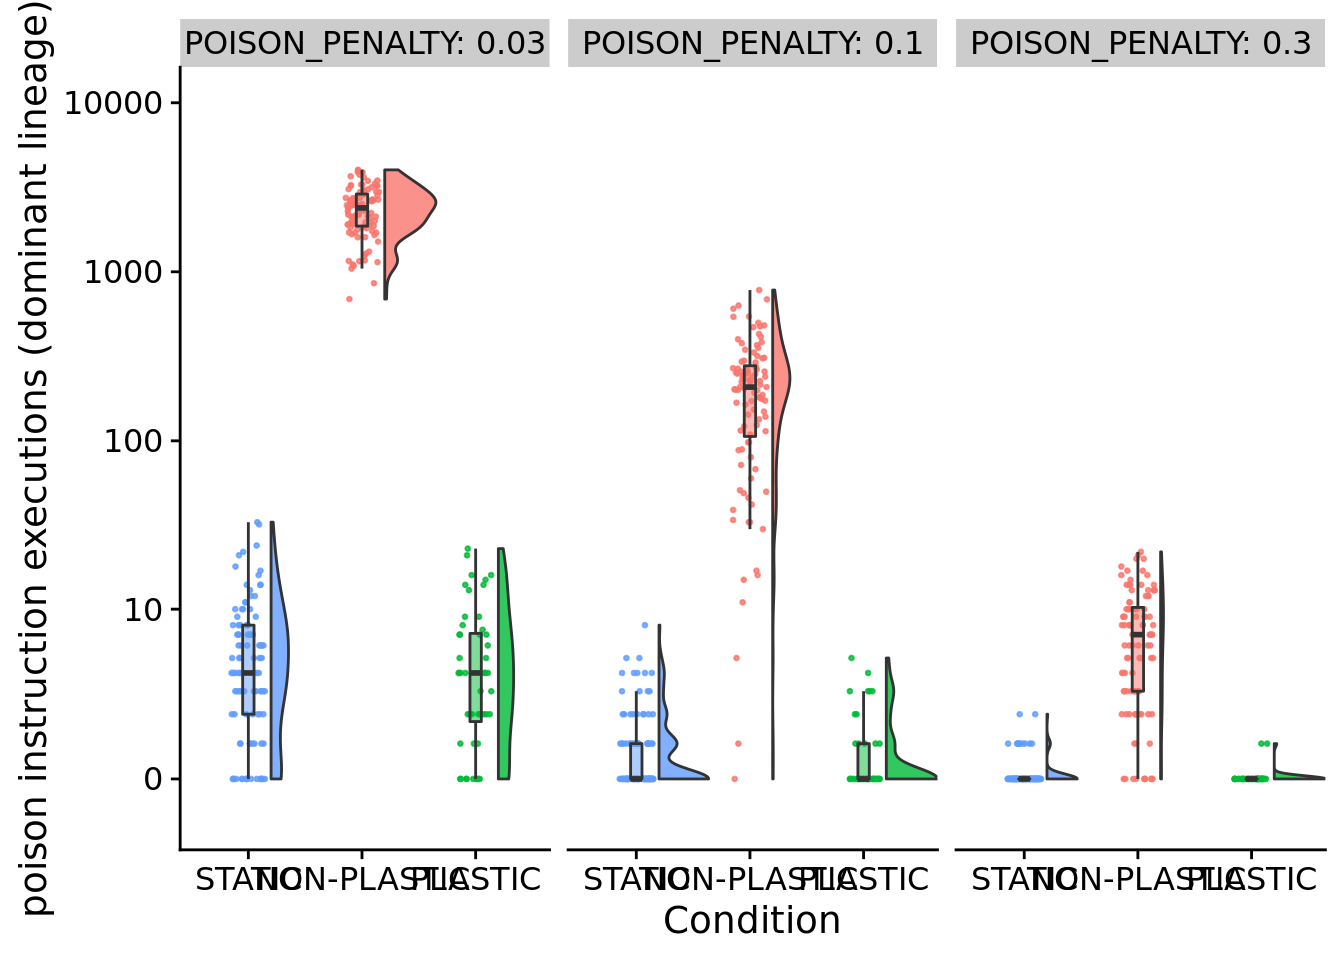
\includegraphics{supplemental-material_files/figure-latex/unnamed-chunk-72-1.pdf}

\begin{Shaded}
\begin{Highlighting}[]
\KeywordTok{paste0}\NormalTok{(}
  \StringTok{"PLASTIC median: "}\NormalTok{,}
  \KeywordTok{median}\NormalTok{(}\KeywordTok{filter}\NormalTok{(summary_data, condition}\OperatorTok{==}\StringTok{"PLASTIC"}\NormalTok{)}\OperatorTok{$}\NormalTok{dominant_lineage_extra_traits_lost_per_generation)}
\NormalTok{)}
\end{Highlighting}
\end{Shaded}

\begin{verbatim}
## [1] "PLASTIC median: 6.25141973661864e-05"
\end{verbatim}

\begin{Shaded}
\begin{Highlighting}[]
\KeywordTok{paste0}\NormalTok{(}
  \StringTok{"STATIC median: "}\NormalTok{,}
  \KeywordTok{median}\NormalTok{(}\KeywordTok{filter}\NormalTok{(summary_data, condition}\OperatorTok{==}\StringTok{"STATIC"}\NormalTok{)}\OperatorTok{$}\NormalTok{dominant_lineage_extra_traits_lost_per_generation)}
\NormalTok{)}
\end{Highlighting}
\end{Shaded}

\begin{verbatim}
## [1] "STATIC median: 0.000161396283669756"
\end{verbatim}

\begin{Shaded}
\begin{Highlighting}[]
\KeywordTok{paste0}\NormalTok{(}
  \StringTok{"NON-PLASTIC median: "}\NormalTok{,}
  \KeywordTok{median}\NormalTok{(}\KeywordTok{filter}\NormalTok{(summary_data, condition}\OperatorTok{==}\StringTok{"NON-PLASTIC"}\NormalTok{)}\OperatorTok{$}\NormalTok{dominant_lineage_extra_traits_lost_per_generation)}
\NormalTok{)}
\end{Highlighting}
\end{Shaded}

\begin{verbatim}
## [1] "NON-PLASTIC median: 0.0022026054610079"
\end{verbatim}

\begin{Shaded}
\begin{Highlighting}[]
\NormalTok{reward_level <-}\StringTok{ }\FloatTok{0.1}
\NormalTok{dom_task_data <-}\StringTok{ }\KeywordTok{filter}\NormalTok{(summary_data, extra_task_value}\OperatorTok{==}\NormalTok{reward_level)}
\KeywordTok{kruskal.test}\NormalTok{(}
  \DataTypeTok{formula=}\NormalTok{dominant_lineage_extra_traits_lost_per_generation}\OperatorTok{~}\NormalTok{condition,}
  \DataTypeTok{data=}\NormalTok{dom_task_data}
\NormalTok{)}
\end{Highlighting}
\end{Shaded}

\begin{verbatim}
## 
##  Kruskal-Wallis rank sum test
## 
## data:  dominant_lineage_extra_traits_lost_per_generation by condition
## Kruskal-Wallis chi-squared = 121.41, df = 2, p-value < 2.2e-16
\end{verbatim}

\begin{Shaded}
\begin{Highlighting}[]
\KeywordTok{pairwise.wilcox.test}\NormalTok{(}
  \DataTypeTok{x=}\NormalTok{dom_task_data}\OperatorTok{$}\NormalTok{dominant_lineage_extra_traits_lost_per_generation,}
  \DataTypeTok{g=}\NormalTok{dom_task_data}\OperatorTok{$}\NormalTok{condition,}
  \DataTypeTok{p.adjust.method=}\StringTok{"bonferroni"}\NormalTok{,}
  \DataTypeTok{conf.int=}\OtherTok{TRUE}\NormalTok{,}
  \DataTypeTok{conf.level=}\FloatTok{0.95}
\NormalTok{)}
\end{Highlighting}
\end{Shaded}

\begin{verbatim}
## 
##  Pairwise comparisons using Wilcoxon rank sum test with continuity correction 
## 
## data:  dom_task_data$dominant_lineage_extra_traits_lost_per_generation and dom_task_data$condition 
## 
##         NON-PLASTIC PLASTIC
## PLASTIC 1.1e-15     -      
## STATIC  < 2e-16     0.0012 
## 
## P value adjustment method: bonferroni
\end{verbatim}

\hypertarget{how-many-instances-of-novel-trait-loss-co-occur-with-changes-in-base-phenotype}{%
\subsubsection{How many instances of novel trait loss co-occur with changes in base phenotype?}\label{how-many-instances-of-novel-trait-loss-co-occur-with-changes-in-base-phenotype}}

Task loss linked with primary trait changes.

\begin{Shaded}
\begin{Highlighting}[]
\NormalTok{lost_traits_summary_data <-}\StringTok{ }\KeywordTok{filter}\NormalTok{(summary_data, extra_task_value}\OperatorTok{==}\FloatTok{0.1} \OperatorTok{&}\StringTok{ }\NormalTok{dominant_lineage_extra_traits_lost}\OperatorTok{>}\DecValTok{0}\NormalTok{)}
\NormalTok{lost_traits_summary_data}\OperatorTok{$}\NormalTok{frac_linked_extra_trait_loss <-}\StringTok{ }\NormalTok{lost_traits_summary_data}\OperatorTok{$}\NormalTok{dominant_lineage_extra_traits_lost_linked_to_primary_change }\OperatorTok{/}\StringTok{ }\NormalTok{lost_traits_summary_data}\OperatorTok{$}\NormalTok{dominant_lineage_extra_traits_lost}

\KeywordTok{ggplot}\NormalTok{(lost_traits_summary_data, }\KeywordTok{aes}\NormalTok{(}\DataTypeTok{x=}\NormalTok{frac_linked_extra_trait_loss)) }\OperatorTok{+}
\StringTok{  }\KeywordTok{geom_density}\NormalTok{() }\OperatorTok{+}
\StringTok{  }\KeywordTok{facet_grid}\NormalTok{(}
\NormalTok{    condition}\OperatorTok{~}\NormalTok{extra_task_value,}
    \DataTypeTok{labeller=}\NormalTok{label_both}
\NormalTok{  ) }\OperatorTok{+}
\StringTok{  }\KeywordTok{theme}\NormalTok{(}
    \DataTypeTok{legend.position=}\StringTok{"none"}
\NormalTok{  ) }\OperatorTok{+}
\StringTok{  }\KeywordTok{ggsave}\NormalTok{(}
    \KeywordTok{paste0}\NormalTok{(working_directory, }\StringTok{"plots/dominant-lineage-extra-tasks-lost-linkage.pdf"}\NormalTok{),}
    \DataTypeTok{width=}\DecValTok{15}\NormalTok{,}
    \DataTypeTok{height=}\DecValTok{10}
\NormalTok{  )}
\end{Highlighting}
\end{Shaded}

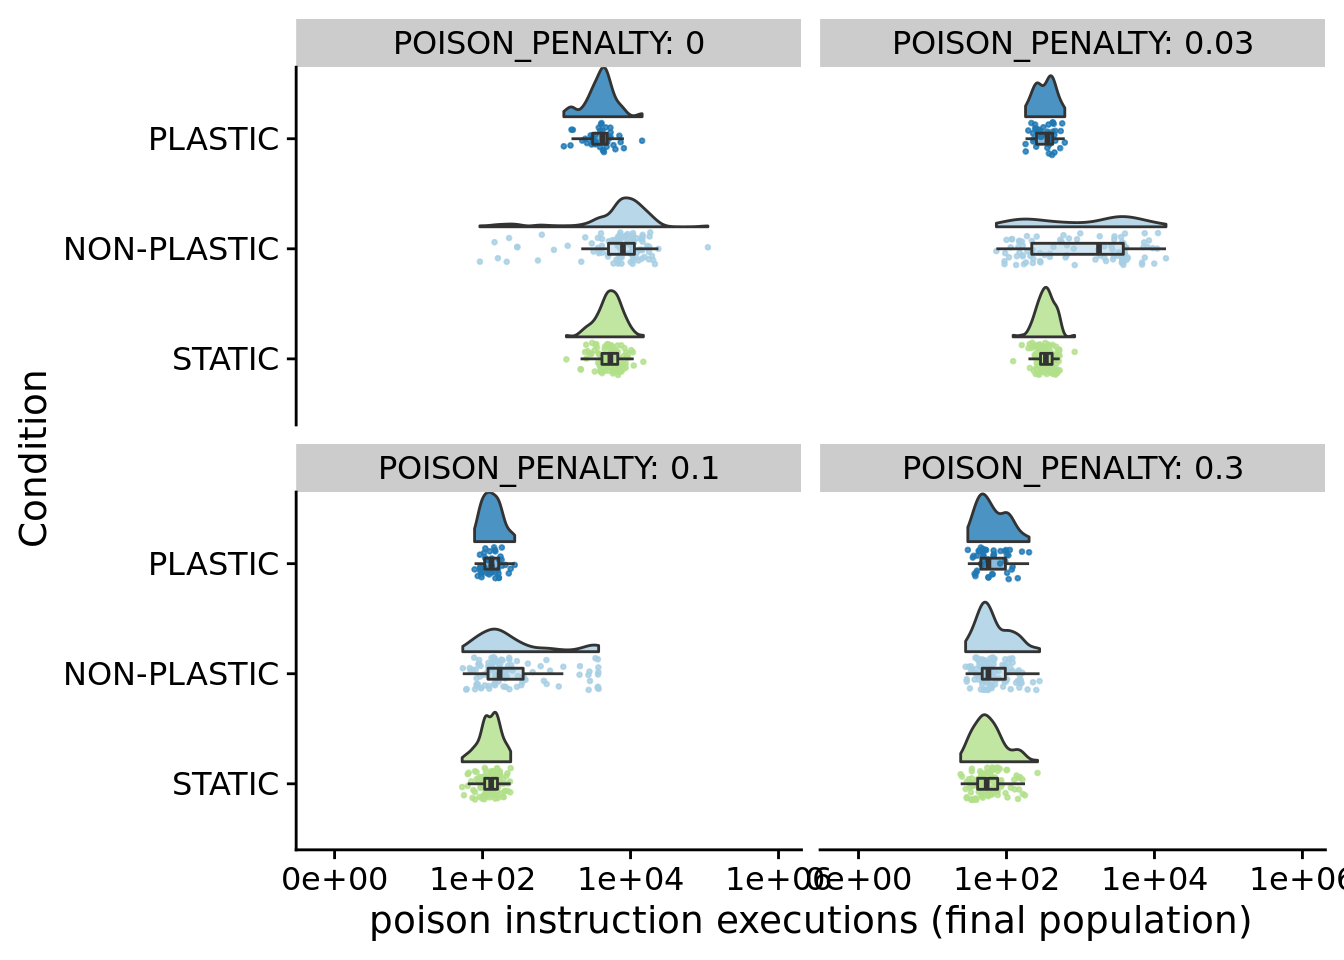
\includegraphics{supplemental-material_files/figure-latex/unnamed-chunk-74-1.pdf}

\begin{Shaded}
\begin{Highlighting}[]
\KeywordTok{ggplot}\NormalTok{(lost_traits_summary_data, }\KeywordTok{aes}\NormalTok{(}\DataTypeTok{x=}\NormalTok{condition, }\DataTypeTok{y=}\NormalTok{frac_linked_extra_trait_loss, }\DataTypeTok{fill=}\NormalTok{condition)) }\OperatorTok{+}
\StringTok{  }\KeywordTok{geom_flat_violin}\NormalTok{(}
    \DataTypeTok{position =} \KeywordTok{position_nudge}\NormalTok{(}\DataTypeTok{x =} \FloatTok{.2}\NormalTok{, }\DataTypeTok{y =} \DecValTok{0}\NormalTok{),}
    \DataTypeTok{alpha =} \FloatTok{.8}
\NormalTok{  ) }\OperatorTok{+}
\StringTok{  }\KeywordTok{geom_point}\NormalTok{(}
    \DataTypeTok{mapping=}\KeywordTok{aes}\NormalTok{(}\DataTypeTok{color=}\NormalTok{condition),}
    \DataTypeTok{position =} \KeywordTok{position_jitter}\NormalTok{(}\DataTypeTok{width =} \FloatTok{.15}\NormalTok{),}
    \DataTypeTok{size =} \FloatTok{.5}\NormalTok{,}
    \DataTypeTok{alpha =} \FloatTok{0.8}
\NormalTok{  ) }\OperatorTok{+}
\StringTok{  }\KeywordTok{geom_boxplot}\NormalTok{(}
    \DataTypeTok{width =} \FloatTok{.1}\NormalTok{,}
    \DataTypeTok{outlier.shape =} \OtherTok{NA}\NormalTok{,}
    \DataTypeTok{alpha =} \FloatTok{0.5}
\NormalTok{  ) }\OperatorTok{+}
\StringTok{  }\KeywordTok{scale_x_discrete}\NormalTok{(}
    \DataTypeTok{name=}\StringTok{"Condition"}\NormalTok{,}
    \DataTypeTok{limits=}\NormalTok{condition_order}
\NormalTok{  ) }\OperatorTok{+}
\StringTok{  }\KeywordTok{facet_wrap}\NormalTok{(}
    \OperatorTok{~}\NormalTok{extra_task_value,}
    \DataTypeTok{labeller=}\NormalTok{label_both}
\NormalTok{  ) }\OperatorTok{+}
\StringTok{  }\KeywordTok{theme}\NormalTok{(}
    \DataTypeTok{legend.position=}\StringTok{"none"}
\NormalTok{  )}
\end{Highlighting}
\end{Shaded}

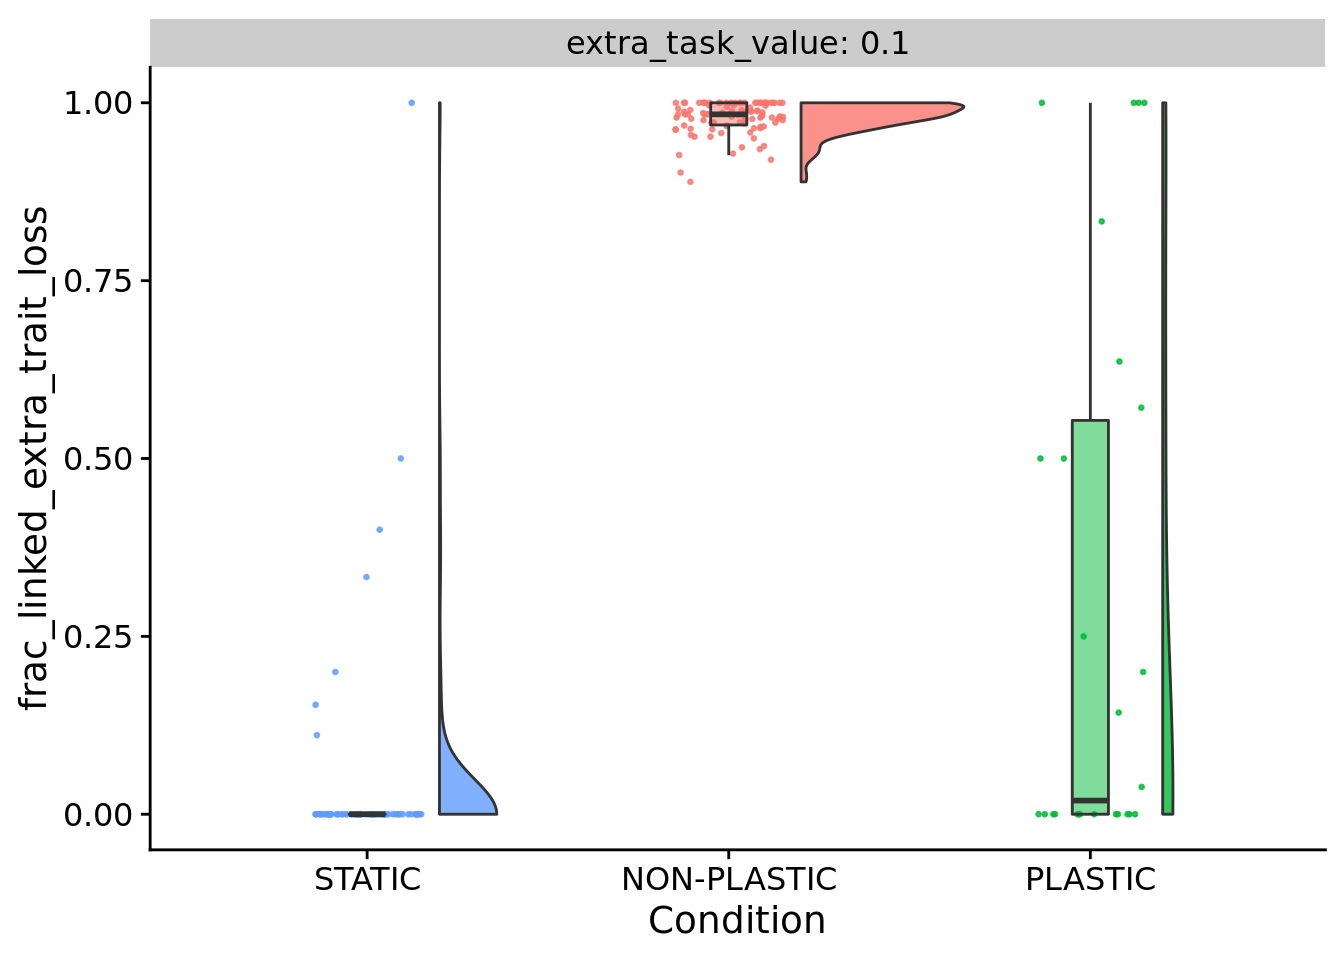
\includegraphics{supplemental-material_files/figure-latex/unnamed-chunk-75-1.pdf}

\begin{Shaded}
\begin{Highlighting}[]
\KeywordTok{paste0}\NormalTok{(}
  \StringTok{"PLASTIC median: "}\NormalTok{,}
  \KeywordTok{median}\NormalTok{(}\KeywordTok{filter}\NormalTok{(lost_traits_summary_data, condition}\OperatorTok{==}\StringTok{"PLASTIC"}\NormalTok{)}\OperatorTok{$}\NormalTok{frac_linked_extra_trait_loss)}
\NormalTok{)}
\end{Highlighting}
\end{Shaded}

\begin{verbatim}
## [1] "PLASTIC median: 0.0192307692307692"
\end{verbatim}

\begin{Shaded}
\begin{Highlighting}[]
\KeywordTok{paste0}\NormalTok{(}
  \StringTok{"STATIC median: "}\NormalTok{,}
  \KeywordTok{median}\NormalTok{(}\KeywordTok{filter}\NormalTok{(lost_traits_summary_data, condition}\OperatorTok{==}\StringTok{"STATIC"}\NormalTok{)}\OperatorTok{$}\NormalTok{frac_linked_extra_trait_loss)}
\NormalTok{)}
\end{Highlighting}
\end{Shaded}

\begin{verbatim}
## [1] "STATIC median: 0"
\end{verbatim}

\begin{Shaded}
\begin{Highlighting}[]
\KeywordTok{paste0}\NormalTok{(}
  \StringTok{"NON-PLASTIC median: "}\NormalTok{,}
  \KeywordTok{median}\NormalTok{(}\KeywordTok{filter}\NormalTok{(lost_traits_summary_data, condition}\OperatorTok{==}\StringTok{"NON-PLASTIC"}\NormalTok{)}\OperatorTok{$}\NormalTok{frac_linked_extra_trait_loss)}
\NormalTok{)}
\end{Highlighting}
\end{Shaded}

\begin{verbatim}
## [1] "NON-PLASTIC median: 0.983803278688525"
\end{verbatim}

\begin{Shaded}
\begin{Highlighting}[]
\KeywordTok{kruskal.test}\NormalTok{(}
  \DataTypeTok{formula=}\NormalTok{frac_linked_extra_trait_loss}\OperatorTok{~}\NormalTok{condition,}
  \DataTypeTok{data=}\NormalTok{lost_traits_summary_data}
\NormalTok{)}
\end{Highlighting}
\end{Shaded}

\begin{verbatim}
## 
##  Kruskal-Wallis rank sum test
## 
## data:  frac_linked_extra_trait_loss by condition
## Kruskal-Wallis chi-squared = 153.68, df = 2, p-value < 2.2e-16
\end{verbatim}

\begin{Shaded}
\begin{Highlighting}[]
\KeywordTok{pairwise.wilcox.test}\NormalTok{(}
  \DataTypeTok{x=}\NormalTok{lost_traits_summary_data}\OperatorTok{$}\NormalTok{frac_linked_extra_trait_loss,}
  \DataTypeTok{g=}\NormalTok{lost_traits_summary_data}\OperatorTok{$}\NormalTok{condition,}
  \DataTypeTok{p.adjust.method=}\StringTok{"bonferroni"}\NormalTok{,}
  \DataTypeTok{conf.int=}\OtherTok{TRUE}\NormalTok{,}
  \DataTypeTok{conf.level=}\FloatTok{0.95}
\NormalTok{)}
\end{Highlighting}
\end{Shaded}

\begin{verbatim}
## 
##  Pairwise comparisons using Wilcoxon rank sum test with continuity correction 
## 
## data:  lost_traits_summary_data$frac_linked_extra_trait_loss and lost_traits_summary_data$condition 
## 
##         NON-PLASTIC PLASTIC
## PLASTIC 1.9e-08     -      
## STATIC  < 2e-16     1.8e-06
## 
## P value adjustment method: bonferroni
\end{verbatim}

\begin{Shaded}
\begin{Highlighting}[]
\KeywordTok{sum}\NormalTok{(}\KeywordTok{filter}\NormalTok{(lost_traits_summary_data, condition}\OperatorTok{==}\StringTok{"NON-PLASTIC"}\NormalTok{)}\OperatorTok{$}\NormalTok{dominant_lineage_extra_traits_lost_linked_to_primary_change)}
\end{Highlighting}
\end{Shaded}

\begin{verbatim}
## [1] 10998
\end{verbatim}

\begin{Shaded}
\begin{Highlighting}[]
\KeywordTok{sum}\NormalTok{(}\KeywordTok{filter}\NormalTok{(lost_traits_summary_data, condition}\OperatorTok{==}\StringTok{"NON-PLASTIC"}\NormalTok{)}\OperatorTok{$}\NormalTok{dominant_lineage_extra_traits_lost)}
\end{Highlighting}
\end{Shaded}

\begin{verbatim}
## [1] 11229
\end{verbatim}

\begin{Shaded}
\begin{Highlighting}[]
\NormalTok{aggregate_frac_linked_extra_trait_loss_nonplastic <-}\StringTok{ }\KeywordTok{sum}\NormalTok{(}\KeywordTok{filter}\NormalTok{(lost_traits_summary_data, condition}\OperatorTok{==}\StringTok{"NON-PLASTIC"}\NormalTok{)}\OperatorTok{$}\NormalTok{dominant_lineage_extra_traits_lost_linked_to_primary_change) }\OperatorTok{/}\StringTok{ }\KeywordTok{sum}\NormalTok{(}\KeywordTok{filter}\NormalTok{(lost_traits_summary_data, condition}\OperatorTok{==}\StringTok{"NON-PLASTIC"}\NormalTok{)}\OperatorTok{$}\NormalTok{dominant_lineage_extra_traits_lost)}
\NormalTok{aggregate_frac_linked_extra_trait_loss_nonplastic}
\end{Highlighting}
\end{Shaded}

\begin{verbatim}
## [1] 0.9794283
\end{verbatim}

\begin{Shaded}
\begin{Highlighting}[]
\KeywordTok{sum}\NormalTok{(}\KeywordTok{filter}\NormalTok{(lost_traits_summary_data, condition}\OperatorTok{==}\StringTok{"PLASTIC"}\NormalTok{)}\OperatorTok{$}\NormalTok{dominant_lineage_extra_traits_lost_linked_to_primary_change)}
\end{Highlighting}
\end{Shaded}

\begin{verbatim}
## [1] 29
\end{verbatim}

\begin{Shaded}
\begin{Highlighting}[]
\KeywordTok{sum}\NormalTok{(}\KeywordTok{filter}\NormalTok{(lost_traits_summary_data, condition}\OperatorTok{==}\StringTok{"PLASTIC"}\NormalTok{)}\OperatorTok{$}\NormalTok{dominant_lineage_extra_traits_lost)}
\end{Highlighting}
\end{Shaded}

\begin{verbatim}
## [1] 142
\end{verbatim}

\begin{Shaded}
\begin{Highlighting}[]
\NormalTok{aggregate_frac_linked_extra_trait_loss_plastic <-}\StringTok{ }\KeywordTok{sum}\NormalTok{(}\KeywordTok{filter}\NormalTok{(lost_traits_summary_data, condition}\OperatorTok{==}\StringTok{"PLASTIC"}\NormalTok{)}\OperatorTok{$}\NormalTok{dominant_lineage_extra_traits_lost_linked_to_primary_change) }\OperatorTok{/}\StringTok{ }\KeywordTok{sum}\NormalTok{(}\KeywordTok{filter}\NormalTok{(lost_traits_summary_data, condition}\OperatorTok{==}\StringTok{"PLASTIC"}\NormalTok{)}\OperatorTok{$}\NormalTok{dominant_lineage_extra_traits_lost)}
\NormalTok{aggregate_frac_linked_extra_trait_loss_plastic}
\end{Highlighting}
\end{Shaded}

\begin{verbatim}
## [1] 0.2042254
\end{verbatim}

\begin{Shaded}
\begin{Highlighting}[]
\KeywordTok{sum}\NormalTok{(}\KeywordTok{filter}\NormalTok{(lost_traits_summary_data, condition}\OperatorTok{==}\StringTok{"STATIC"}\NormalTok{)}\OperatorTok{$}\NormalTok{dominant_lineage_extra_traits_lost_linked_to_primary_change)}
\end{Highlighting}
\end{Shaded}

\begin{verbatim}
## [1] 13
\end{verbatim}

\begin{Shaded}
\begin{Highlighting}[]
\KeywordTok{sum}\NormalTok{(}\KeywordTok{filter}\NormalTok{(lost_traits_summary_data, condition}\OperatorTok{==}\StringTok{"STATIC"}\NormalTok{)}\OperatorTok{$}\NormalTok{dominant_lineage_extra_traits_lost)}
\end{Highlighting}
\end{Shaded}

\begin{verbatim}
## [1] 631
\end{verbatim}

\begin{Shaded}
\begin{Highlighting}[]
\NormalTok{aggregate_frac_linked_extra_trait_loss_nonplastic <-}\StringTok{ }\KeywordTok{sum}\NormalTok{(}\KeywordTok{filter}\NormalTok{(lost_traits_summary_data, condition}\OperatorTok{==}\StringTok{"STATIC"}\NormalTok{)}\OperatorTok{$}\NormalTok{dominant_lineage_extra_traits_lost_linked_to_primary_change) }\OperatorTok{/}\StringTok{ }\KeywordTok{sum}\NormalTok{(}\KeywordTok{filter}\NormalTok{(lost_traits_summary_data, condition}\OperatorTok{==}\StringTok{"STATIC"}\NormalTok{)}\OperatorTok{$}\NormalTok{dominant_lineage_extra_traits_lost)}
\NormalTok{aggregate_frac_linked_extra_trait_loss_nonplastic}
\end{Highlighting}
\end{Shaded}

\begin{verbatim}
## [1] 0.02060222
\end{verbatim}

\hypertarget{extra-task-performance-over-time}{%
\section{Extra task performance over time}\label{extra-task-performance-over-time}}

Match score over time

\begin{Shaded}
\begin{Highlighting}[]
\NormalTok{lineage_reward10 <-}\StringTok{ }\KeywordTok{filter}\NormalTok{(lineage_time_series_data, extra_task_value}\OperatorTok{==}\StringTok{"0.1"}\NormalTok{)}

\KeywordTok{ggplot}\NormalTok{(}\KeywordTok{filter}\NormalTok{(lineage_reward10, update}\OperatorTok{>}\DecValTok{198000} \OperatorTok{&}\StringTok{ }\NormalTok{update}\OperatorTok{<=}\DecValTok{200000}\NormalTok{), }\KeywordTok{aes}\NormalTok{(}\DataTypeTok{x=}\NormalTok{update, }\DataTypeTok{y=}\NormalTok{match_score_even, }\DataTypeTok{color=}\NormalTok{condition, }\DataTypeTok{fill=}\NormalTok{condition)) }\OperatorTok{+}
\StringTok{  }\KeywordTok{stat_summary}\NormalTok{(}\DataTypeTok{fun=}\StringTok{"mean"}\NormalTok{, }\DataTypeTok{geom=}\StringTok{"line"}\NormalTok{) }\OperatorTok{+}
\StringTok{  }\KeywordTok{stat_summary}\NormalTok{(}
    \DataTypeTok{fun.data=}\StringTok{"mean_cl_boot"}\NormalTok{,}
    \DataTypeTok{fun.args=}\KeywordTok{list}\NormalTok{(}\DataTypeTok{conf.int=}\FloatTok{0.95}\NormalTok{),}
    \DataTypeTok{geom=}\StringTok{"ribbon"}\NormalTok{,}
    \DataTypeTok{alpha=}\FloatTok{0.2}\NormalTok{,}
    \DataTypeTok{linetype=}\DecValTok{0}
\NormalTok{  ) }\OperatorTok{+}
\StringTok{  }\KeywordTok{ylab}\NormalTok{(}\StringTok{"Match score (even environment)"}\NormalTok{) }\OperatorTok{+}
\StringTok{  }\KeywordTok{facet_wrap}\NormalTok{(}
    \OperatorTok{~}\NormalTok{extra_task_value,}
    \DataTypeTok{labeller=}\NormalTok{label_both}
\NormalTok{  ) }\OperatorTok{+}
\StringTok{  }\KeywordTok{ggsave}\NormalTok{(}
    \KeywordTok{paste0}\NormalTok{(working_directory, }\StringTok{"plots/dominant-lineage-match-score-even-val10.png"}\NormalTok{),}
    \DataTypeTok{width=}\DecValTok{15}\NormalTok{,}
    \DataTypeTok{height=}\DecValTok{10}
\NormalTok{  )}
\end{Highlighting}
\end{Shaded}

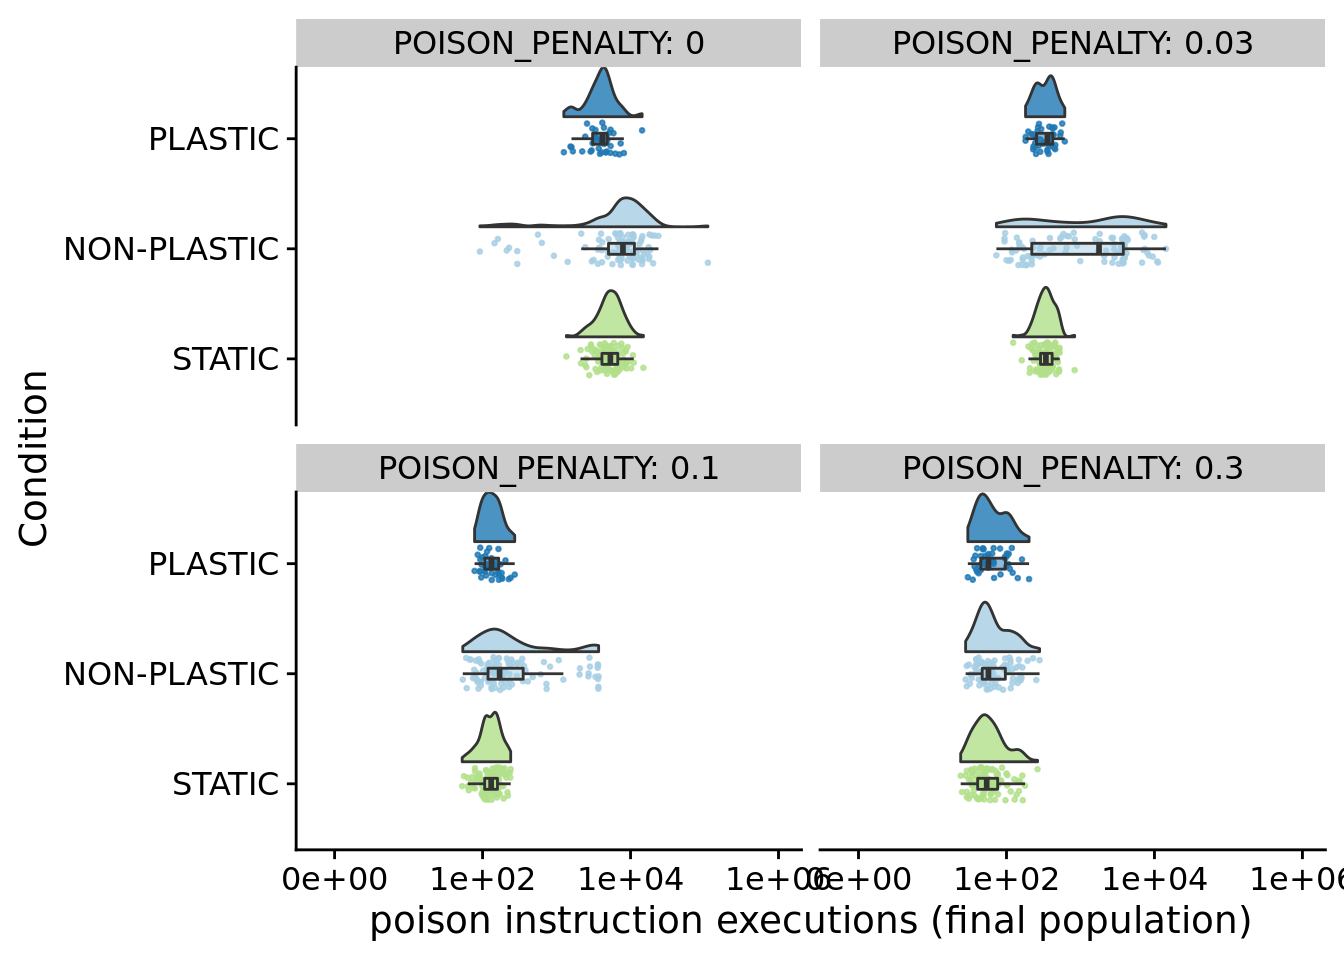
\includegraphics{supplemental-material_files/figure-latex/unnamed-chunk-79-1.pdf}

Extra tasks over time

\begin{Shaded}
\begin{Highlighting}[]
\KeywordTok{ggplot}\NormalTok{(}\KeywordTok{filter}\NormalTok{(lineage_reward10, update}\OperatorTok{>}\DecValTok{198000} \OperatorTok{&}\StringTok{ }\NormalTok{update}\OperatorTok{<=}\DecValTok{200000}\NormalTok{), }\KeywordTok{aes}\NormalTok{(}\DataTypeTok{x=}\NormalTok{update, }\DataTypeTok{y=}\NormalTok{extra_traits, }\DataTypeTok{color=}\NormalTok{condition, }\DataTypeTok{fill=}\NormalTok{condition)) }\OperatorTok{+}
\StringTok{  }\KeywordTok{stat_summary}\NormalTok{(}\DataTypeTok{fun=}\StringTok{"mean"}\NormalTok{, }\DataTypeTok{geom=}\StringTok{"line"}\NormalTok{) }\OperatorTok{+}
\StringTok{  }\KeywordTok{stat_summary}\NormalTok{(}
    \DataTypeTok{fun.data=}\StringTok{"mean_cl_boot"}\NormalTok{,}
    \DataTypeTok{fun.args=}\KeywordTok{list}\NormalTok{(}\DataTypeTok{conf.int=}\FloatTok{0.95}\NormalTok{),}
    \DataTypeTok{geom=}\StringTok{"ribbon"}\NormalTok{,}
    \DataTypeTok{alpha=}\FloatTok{0.2}\NormalTok{,}
    \DataTypeTok{linetype=}\DecValTok{0}
\NormalTok{  ) }\OperatorTok{+}
\StringTok{  }\KeywordTok{ylab}\NormalTok{(}\StringTok{"Number of extra traits"}\NormalTok{) }\OperatorTok{+}
\StringTok{  }\KeywordTok{facet_wrap}\NormalTok{(}
    \OperatorTok{~}\NormalTok{extra_task_value,}
    \DataTypeTok{labeller=}\NormalTok{label_both}
\NormalTok{  ) }\OperatorTok{+}
\StringTok{  }\KeywordTok{ggsave}\NormalTok{(}
    \KeywordTok{paste0}\NormalTok{(working_directory, }\StringTok{"plots/dominant-lineage-extra-traits-val10.png"}\NormalTok{),}
    \DataTypeTok{width=}\DecValTok{15}\NormalTok{,}
    \DataTypeTok{height=}\DecValTok{10}
\NormalTok{  )}
\end{Highlighting}
\end{Shaded}

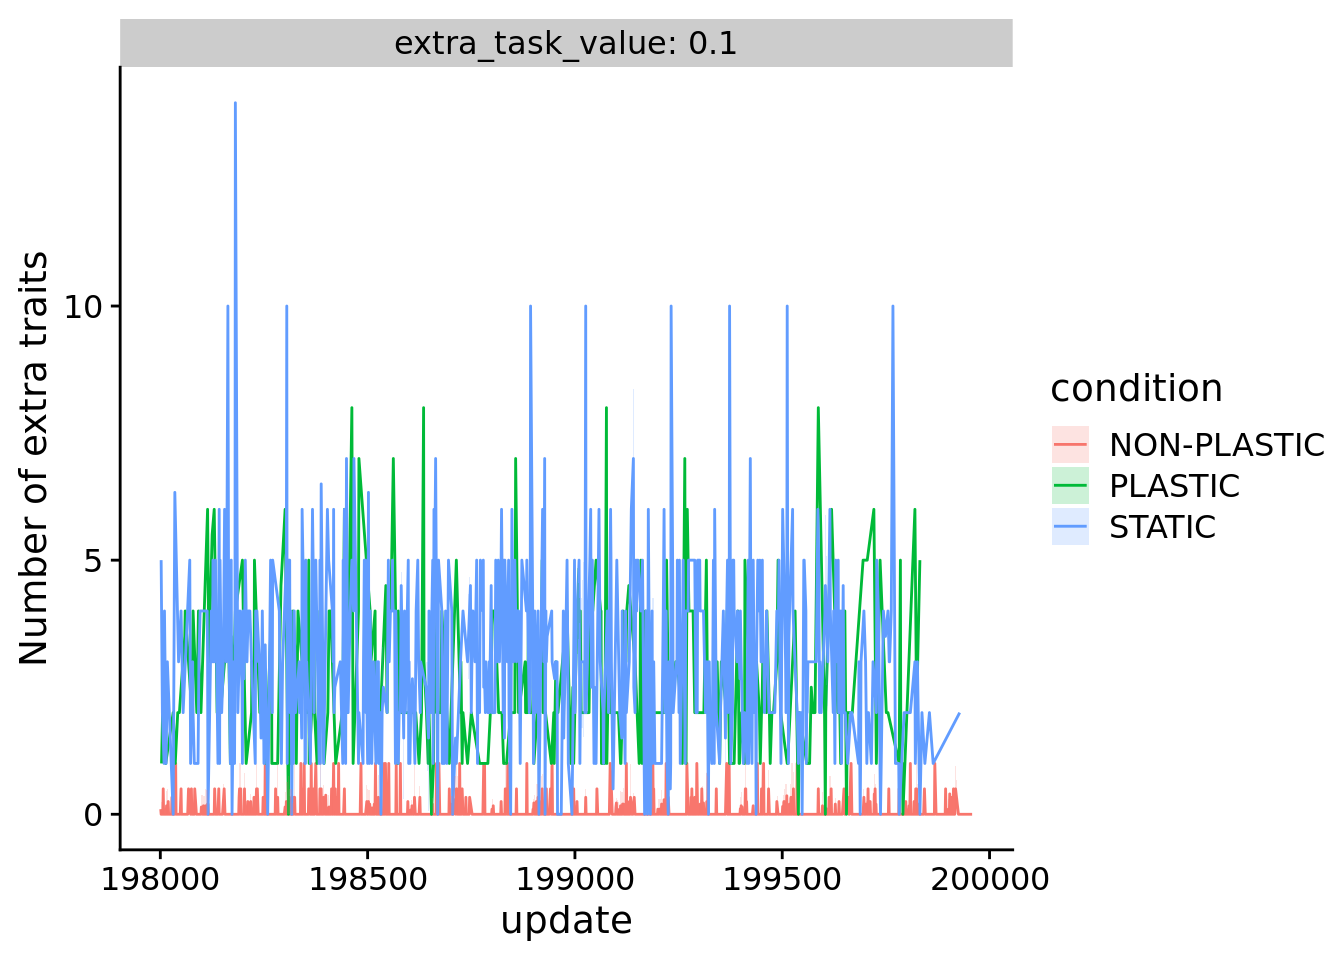
\includegraphics{supplemental-material_files/figure-latex/unnamed-chunk-80-1.pdf}

\hypertarget{manuscript-figures-1}{%
\section{Manuscript figures}\label{manuscript-figures-1}}

Final dominant extra tasks.

\begin{Shaded}
\begin{Highlighting}[]
\NormalTok{extra_task_reward_value=}\FloatTok{0.1}
\NormalTok{dominant_extra_tasks_fig <-}\StringTok{ }\KeywordTok{ggplot}\NormalTok{(}
    \KeywordTok{filter}\NormalTok{(summary_data, extra_task_value}\OperatorTok{==}\NormalTok{extra_task_reward_value),}
    \KeywordTok{aes}\NormalTok{(}\DataTypeTok{x=}\NormalTok{condition, }\DataTypeTok{y=}\NormalTok{dominant_extra_tasks, }\DataTypeTok{fill=}\NormalTok{condition)}
\NormalTok{  ) }\OperatorTok{+}
\StringTok{  }\KeywordTok{geom_flat_violin}\NormalTok{(}
    \DataTypeTok{position =} \KeywordTok{position_nudge}\NormalTok{(}\DataTypeTok{x =} \FloatTok{.2}\NormalTok{, }\DataTypeTok{y =} \DecValTok{0}\NormalTok{),}
    \DataTypeTok{alpha =} \FloatTok{.8}
\NormalTok{  ) }\OperatorTok{+}
\StringTok{  }\KeywordTok{geom_point}\NormalTok{(}
    \DataTypeTok{mapping=}\KeywordTok{aes}\NormalTok{(}\DataTypeTok{color=}\NormalTok{condition),}
    \DataTypeTok{position =} \KeywordTok{position_jitter}\NormalTok{(}\DataTypeTok{width =} \FloatTok{.15}\NormalTok{),}
    \DataTypeTok{size =} \FloatTok{.5}\NormalTok{,}
    \DataTypeTok{alpha =} \FloatTok{0.8}
\NormalTok{  ) }\OperatorTok{+}
\StringTok{  }\KeywordTok{geom_boxplot}\NormalTok{(}
    \DataTypeTok{width =} \FloatTok{.1}\NormalTok{,}
    \DataTypeTok{outlier.shape =} \OtherTok{NA}\NormalTok{,}
    \DataTypeTok{alpha =} \FloatTok{0.5}
\NormalTok{  ) }\OperatorTok{+}
\StringTok{  }\KeywordTok{scale_x_discrete}\NormalTok{(}
    \DataTypeTok{name=}\StringTok{"Condition"}\NormalTok{,}
    \DataTypeTok{limits=}\NormalTok{condition_order,}
    \DataTypeTok{labels=}\NormalTok{condition_order}
\NormalTok{  ) }\OperatorTok{+}
\StringTok{  }\KeywordTok{scale_y_continuous}\NormalTok{(}
    \DataTypeTok{name=}\StringTok{"Final dominant novel traits"}
\NormalTok{  ) }\OperatorTok{+}
\StringTok{  }\KeywordTok{scale_fill_brewer}\NormalTok{(}
    \DataTypeTok{palette=}\StringTok{"Paired"}
\NormalTok{  ) }\OperatorTok{+}
\StringTok{  }\KeywordTok{scale_color_brewer}\NormalTok{(}
    \DataTypeTok{palette=}\StringTok{"Paired"}
\NormalTok{  ) }\OperatorTok{+}
\StringTok{  }\KeywordTok{theme}\NormalTok{(}
    \DataTypeTok{legend.position=}\StringTok{"none"}
\NormalTok{  ) }\OperatorTok{+}
\StringTok{  }\KeywordTok{coord_flip}\NormalTok{()}
\NormalTok{dominant_extra_tasks_fig}
\end{Highlighting}
\end{Shaded}

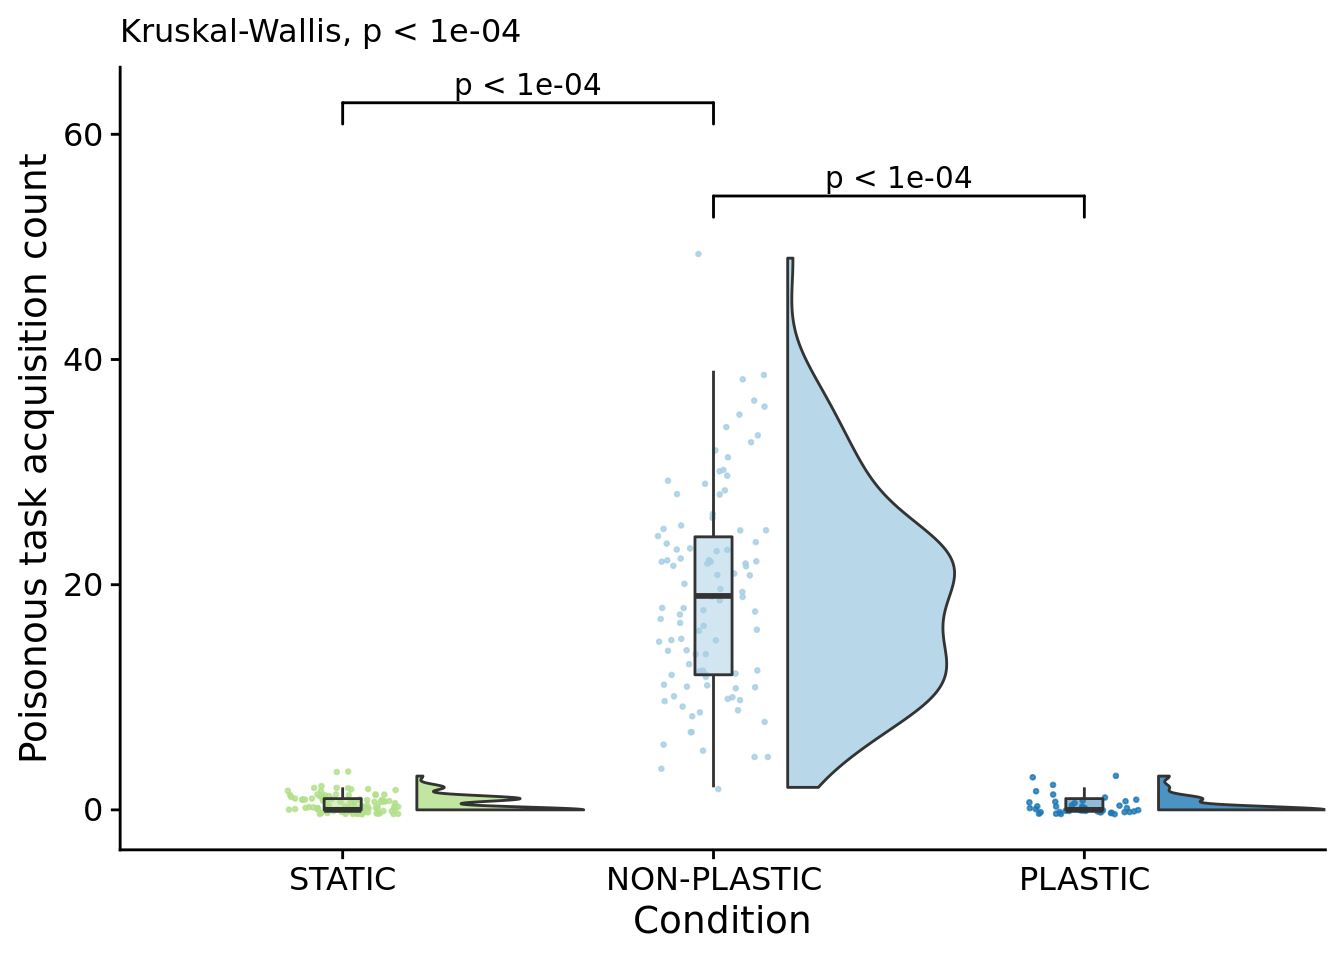
\includegraphics{supplemental-material_files/figure-latex/unnamed-chunk-81-1.pdf}

Final dominant lineage tasks discovered.

\begin{Shaded}
\begin{Highlighting}[]
\NormalTok{lineage_extra_tasks_discovered_fig <-}\StringTok{ }\KeywordTok{ggplot}\NormalTok{(}
    \KeywordTok{filter}\NormalTok{(summary_data, extra_task_value}\OperatorTok{==}\NormalTok{extra_task_reward_value),}
    \KeywordTok{aes}\NormalTok{(}\DataTypeTok{x=}\NormalTok{condition, }\DataTypeTok{y=}\NormalTok{dominant_lineage_extra_traits_discovered, }\DataTypeTok{fill=}\NormalTok{condition)}
\NormalTok{  ) }\OperatorTok{+}
\StringTok{  }\KeywordTok{geom_flat_violin}\NormalTok{(}
    \DataTypeTok{position =} \KeywordTok{position_nudge}\NormalTok{(}\DataTypeTok{x =} \FloatTok{.2}\NormalTok{, }\DataTypeTok{y =} \DecValTok{0}\NormalTok{),}
    \DataTypeTok{alpha =} \FloatTok{.8}
\NormalTok{  ) }\OperatorTok{+}
\StringTok{  }\KeywordTok{geom_point}\NormalTok{(}
    \DataTypeTok{mapping=}\KeywordTok{aes}\NormalTok{(}\DataTypeTok{color=}\NormalTok{condition),}
    \DataTypeTok{position =} \KeywordTok{position_jitter}\NormalTok{(}\DataTypeTok{width =} \FloatTok{.15}\NormalTok{),}
    \DataTypeTok{size =} \FloatTok{.5}\NormalTok{,}
    \DataTypeTok{alpha =} \FloatTok{0.8}
\NormalTok{  ) }\OperatorTok{+}
\StringTok{  }\KeywordTok{geom_boxplot}\NormalTok{(}
    \DataTypeTok{width =} \FloatTok{.1}\NormalTok{,}
    \DataTypeTok{outlier.shape =} \OtherTok{NA}\NormalTok{,}
    \DataTypeTok{alpha =} \FloatTok{0.5}
\NormalTok{  ) }\OperatorTok{+}
\StringTok{  }\KeywordTok{scale_x_discrete}\NormalTok{(}
    \DataTypeTok{name=}\StringTok{"Condition"}\NormalTok{,}
    \DataTypeTok{limits=}\NormalTok{condition_order,}
    \DataTypeTok{labels=}\NormalTok{condition_order}
\NormalTok{  ) }\OperatorTok{+}
\StringTok{  }\KeywordTok{scale_y_continuous}\NormalTok{(}
    \DataTypeTok{name=}\StringTok{"Novel traits discovered on lineage"}
\NormalTok{  ) }\OperatorTok{+}
\StringTok{  }\KeywordTok{scale_fill_brewer}\NormalTok{(}
    \DataTypeTok{palette=}\StringTok{"Paired"}
\NormalTok{  ) }\OperatorTok{+}
\StringTok{  }\KeywordTok{scale_color_brewer}\NormalTok{(}
    \DataTypeTok{palette=}\StringTok{"Paired"}
\NormalTok{  ) }\OperatorTok{+}
\StringTok{  }\KeywordTok{theme}\NormalTok{(}
    \DataTypeTok{legend.position=}\StringTok{"none"}
\NormalTok{  ) }\OperatorTok{+}
\StringTok{  }\KeywordTok{coord_flip}\NormalTok{()}
\NormalTok{lineage_extra_tasks_discovered_fig}
\end{Highlighting}
\end{Shaded}

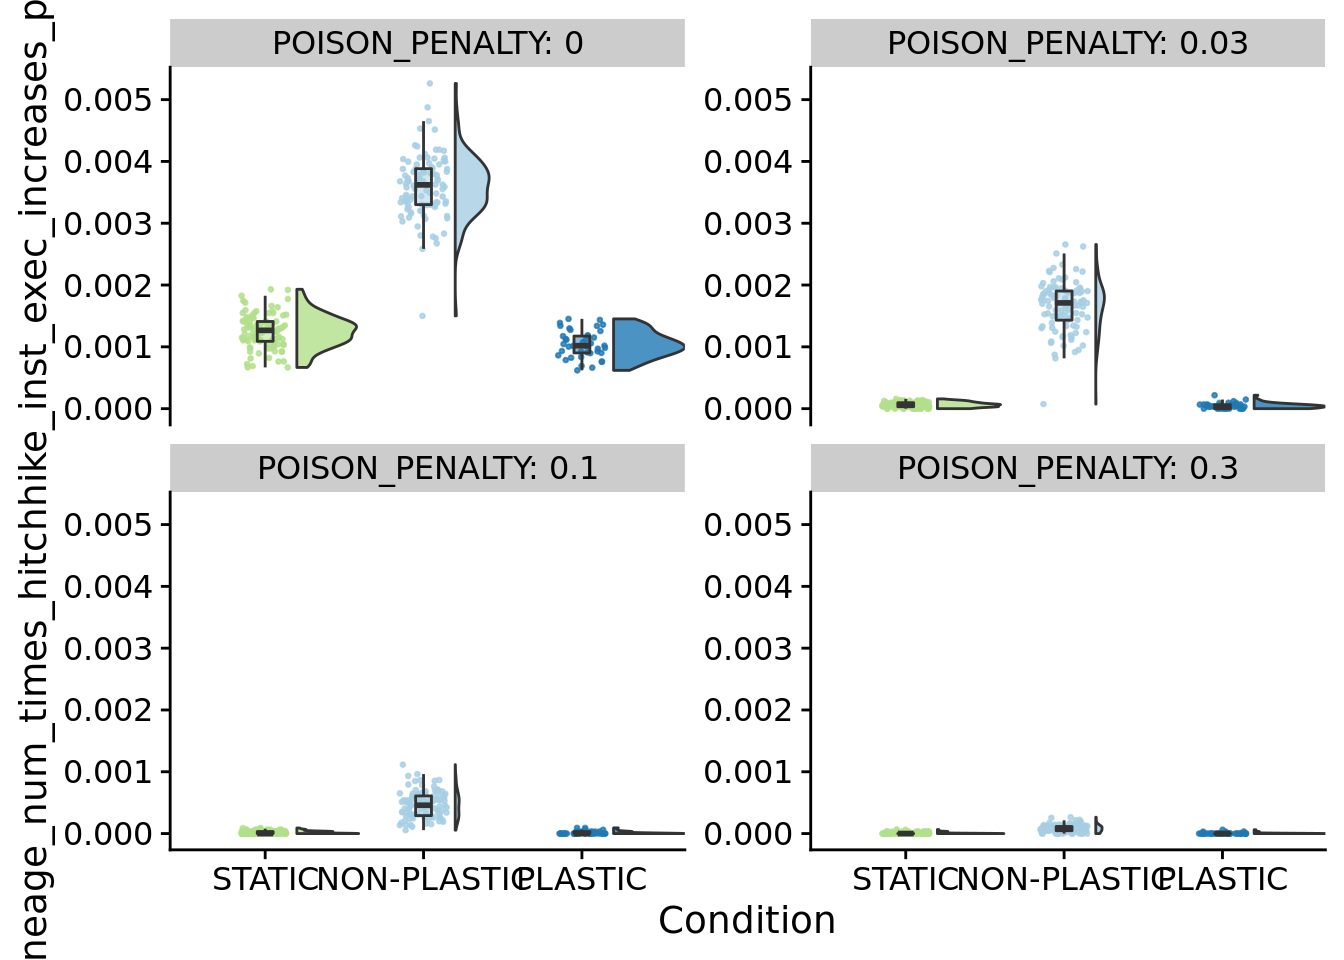
\includegraphics{supplemental-material_files/figure-latex/unnamed-chunk-82-1.pdf}

Final dominant lineage tasks lost.

\begin{Shaded}
\begin{Highlighting}[]
\NormalTok{lineage_extra_tasks_lost_fig <-}\StringTok{ }\KeywordTok{ggplot}\NormalTok{(}
    \KeywordTok{filter}\NormalTok{(summary_data, extra_task_value}\OperatorTok{==}\NormalTok{extra_task_reward_value),}
    \KeywordTok{aes}\NormalTok{(}\DataTypeTok{x=}\NormalTok{condition, }\DataTypeTok{y=}\NormalTok{dominant_lineage_extra_traits_lost, }\DataTypeTok{fill=}\NormalTok{condition)}
\NormalTok{  ) }\OperatorTok{+}
\StringTok{  }\KeywordTok{geom_flat_violin}\NormalTok{(}
    \DataTypeTok{position =} \KeywordTok{position_nudge}\NormalTok{(}\DataTypeTok{x =} \FloatTok{.2}\NormalTok{, }\DataTypeTok{y =} \DecValTok{0}\NormalTok{),}
    \DataTypeTok{alpha =} \FloatTok{.8}
\NormalTok{  ) }\OperatorTok{+}
\StringTok{  }\KeywordTok{geom_point}\NormalTok{(}
    \DataTypeTok{mapping=}\KeywordTok{aes}\NormalTok{(}\DataTypeTok{color=}\NormalTok{condition),}
    \DataTypeTok{position =} \KeywordTok{position_jitter}\NormalTok{(}\DataTypeTok{width =} \FloatTok{.15}\NormalTok{),}
    \DataTypeTok{size =} \FloatTok{.5}\NormalTok{,}
    \DataTypeTok{alpha =} \FloatTok{0.8}
\NormalTok{  ) }\OperatorTok{+}
\StringTok{  }\KeywordTok{geom_boxplot}\NormalTok{(}
    \DataTypeTok{width =} \FloatTok{.1}\NormalTok{,}
    \DataTypeTok{outlier.shape =} \OtherTok{NA}\NormalTok{,}
    \DataTypeTok{alpha =} \FloatTok{0.5}
\NormalTok{  ) }\OperatorTok{+}
\StringTok{  }\KeywordTok{scale_x_discrete}\NormalTok{(}
    \DataTypeTok{name=}\StringTok{"Condition"}\NormalTok{,}
    \DataTypeTok{limits=}\NormalTok{condition_order,}
    \DataTypeTok{labels=}\NormalTok{condition_order}
\NormalTok{  ) }\OperatorTok{+}
\StringTok{  }\KeywordTok{scale_y_continuous}\NormalTok{(}
    \DataTypeTok{name=}\StringTok{"Novel traits lost on lineage (log scale)"}\NormalTok{,}
    \DataTypeTok{trans=}\StringTok{"pseudo_log"}\NormalTok{,}
    \DataTypeTok{breaks=}\KeywordTok{c}\NormalTok{(}\DecValTok{0}\NormalTok{,}\DecValTok{10}\NormalTok{,}\DecValTok{100}\NormalTok{,}\DecValTok{1000}\NormalTok{),}
    \DataTypeTok{limits=}\KeywordTok{c}\NormalTok{(}\OperatorTok{-}\DecValTok{1}\NormalTok{,}\DecValTok{1000}\NormalTok{)}
\NormalTok{  ) }\OperatorTok{+}
\StringTok{  }\KeywordTok{scale_fill_brewer}\NormalTok{(}
    \DataTypeTok{palette=}\StringTok{"Paired"}
\NormalTok{  ) }\OperatorTok{+}
\StringTok{  }\KeywordTok{scale_color_brewer}\NormalTok{(}
    \DataTypeTok{palette=}\StringTok{"Paired"}
\NormalTok{  ) }\OperatorTok{+}
\StringTok{  }\KeywordTok{theme}\NormalTok{(}
    \DataTypeTok{legend.position=}\StringTok{"none"}
\NormalTok{  ) }\OperatorTok{+}
\StringTok{  }\KeywordTok{coord_flip}\NormalTok{()}

\NormalTok{lineage_extra_tasks_lost_fig}
\end{Highlighting}
\end{Shaded}

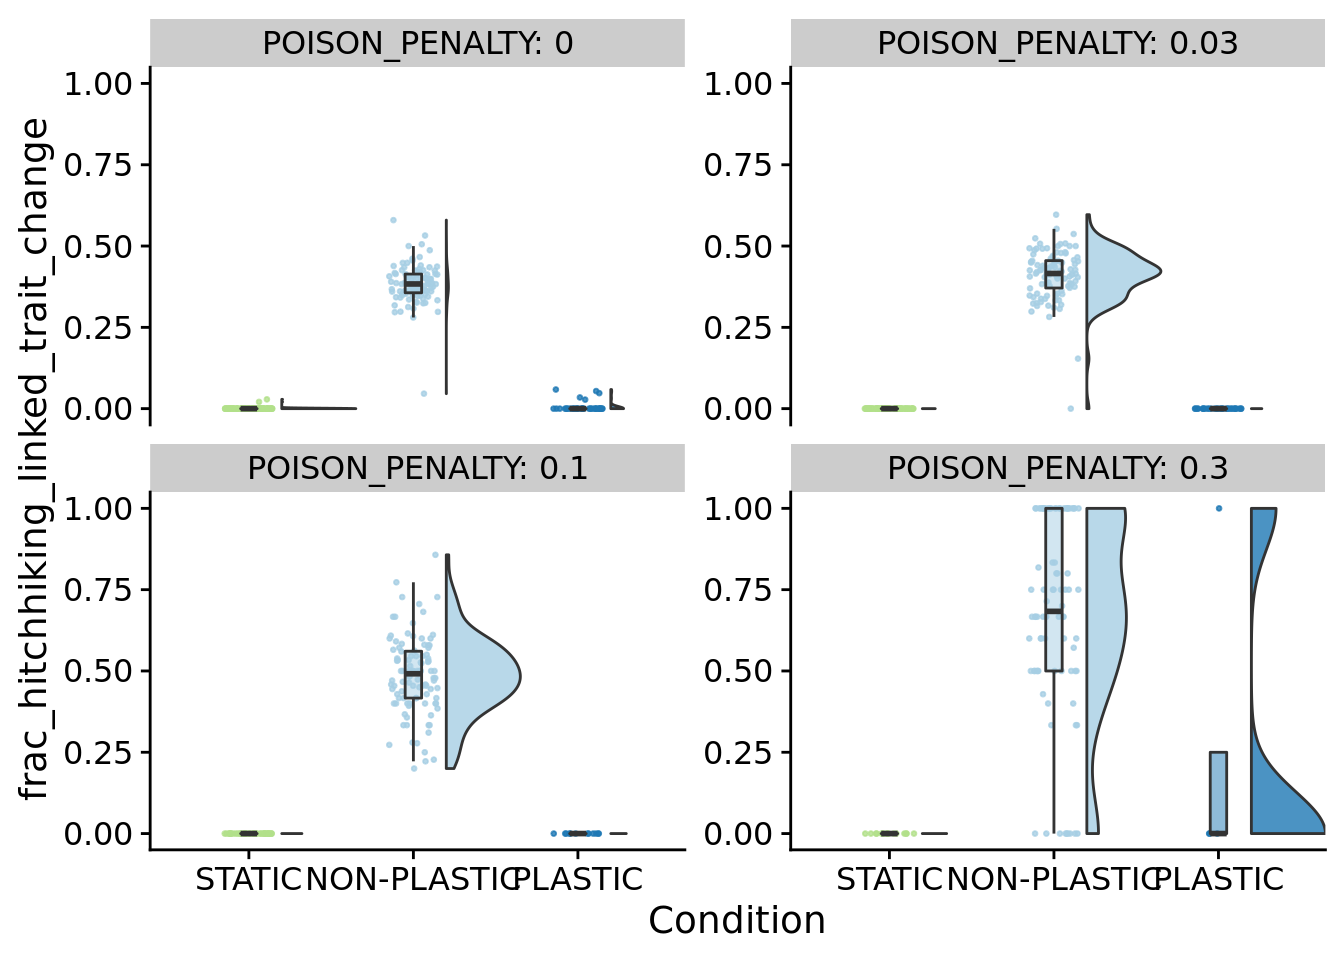
\includegraphics{supplemental-material_files/figure-latex/unnamed-chunk-83-1.pdf}

Pull it all together.

\begin{Shaded}
\begin{Highlighting}[]
\NormalTok{grid <-}\StringTok{ }\KeywordTok{plot_grid}\NormalTok{(}
\NormalTok{  dominant_extra_tasks_fig,}
\NormalTok{  lineage_extra_tasks_discovered_fig }\OperatorTok{+}\StringTok{ }\KeywordTok{theme}\NormalTok{(}\DataTypeTok{axis.ticks.y=}\KeywordTok{element_blank}\NormalTok{(),}\DataTypeTok{axis.text.y=}\KeywordTok{element_blank}\NormalTok{(),}\DataTypeTok{axis.title.y=}\KeywordTok{element_blank}\NormalTok{()),}
\NormalTok{  lineage_extra_tasks_lost_fig }\OperatorTok{+}\StringTok{ }\KeywordTok{theme}\NormalTok{(}\DataTypeTok{axis.ticks.y=}\KeywordTok{element_blank}\NormalTok{(),}\DataTypeTok{axis.text.y=}\KeywordTok{element_blank}\NormalTok{(),}\DataTypeTok{axis.title.y=}\KeywordTok{element_blank}\NormalTok{()),}
  \DataTypeTok{nrow=}\DecValTok{1}\NormalTok{,}
  \DataTypeTok{align=}\StringTok{"v"}\NormalTok{,}
  \DataTypeTok{labels=}\StringTok{"auto"}
\NormalTok{)}
\KeywordTok{save_plot}\NormalTok{(}
   \KeywordTok{paste0}\NormalTok{(working_directory, }\StringTok{"plots/"}\NormalTok{, }\StringTok{"complex-traits-panel.pdf"}\NormalTok{),}
\NormalTok{   grid,}
   \DataTypeTok{base_height=}\DecValTok{6}\NormalTok{,}
   \DataTypeTok{base_asp=}\FloatTok{2.5}
\NormalTok{)}
\NormalTok{grid}
\end{Highlighting}
\end{Shaded}

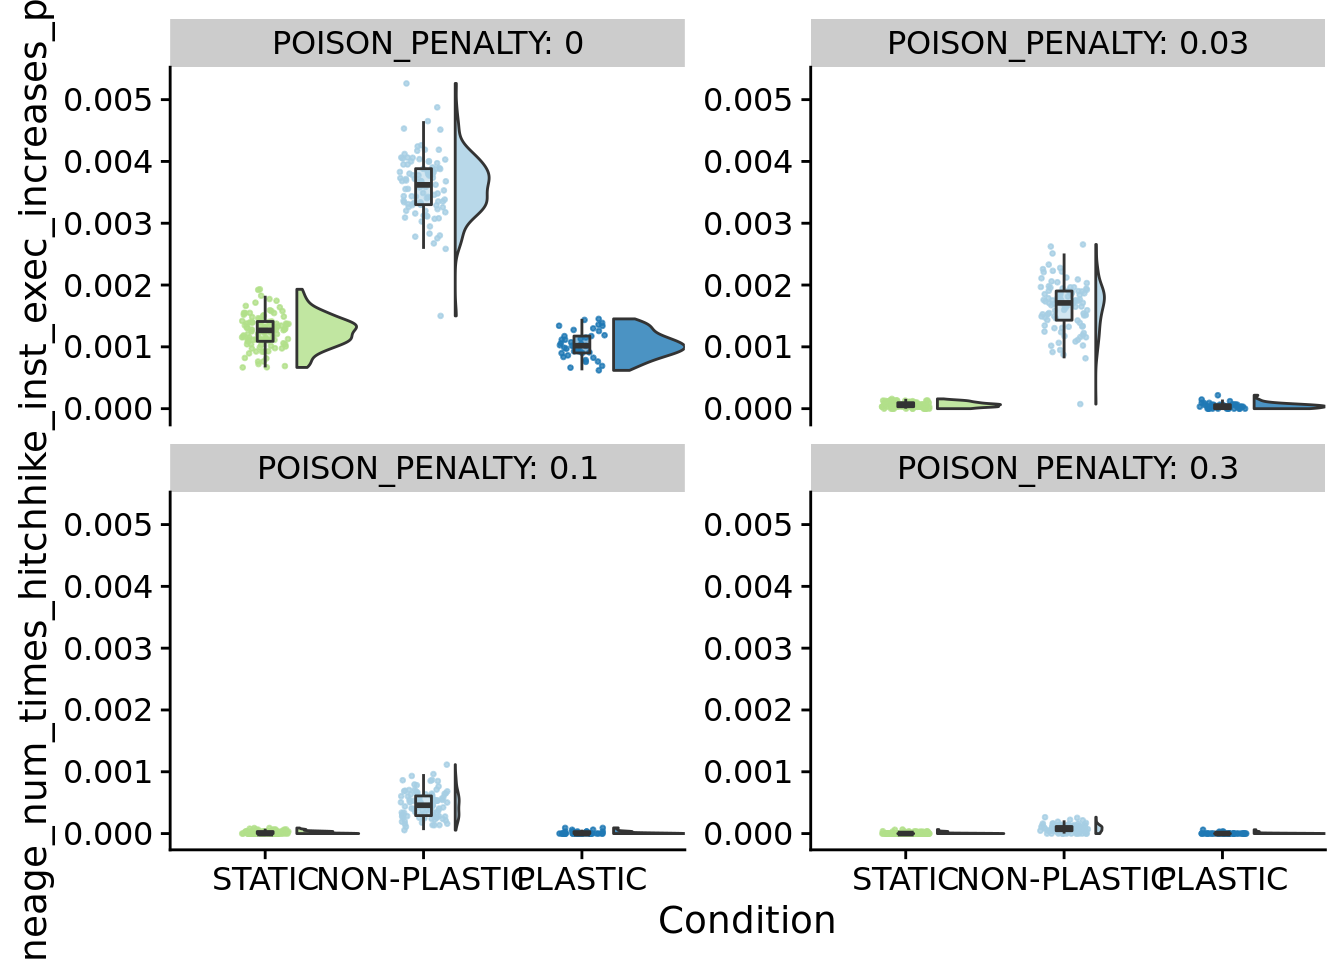
\includegraphics{supplemental-material_files/figure-latex/unnamed-chunk-84-1.pdf}

\hypertarget{genetic-hitchhiking}{%
\chapter{Genetic hitchhiking}\label{genetic-hitchhiking}}

The effect of adaptive phenotypic plasticity on (deleterious) genetic hitchhiking.

\hypertarget{overview-3}{%
\section{Overview}\label{overview-3}}

\begin{Shaded}
\begin{Highlighting}[]
\NormalTok{total_updates <-}\StringTok{ }\DecValTok{200000}
\NormalTok{replicates <-}\StringTok{ }\DecValTok{100}

\NormalTok{focal_traits <-}\StringTok{ }\KeywordTok{c}\NormalTok{(}\StringTok{"not"}\NormalTok{,}\StringTok{"nand"}\NormalTok{,}\StringTok{"and"}\NormalTok{,}\StringTok{"ornot"}\NormalTok{,}\StringTok{"or"}\NormalTok{,}\StringTok{"andnot"}\NormalTok{)}
\NormalTok{traits_set_a <-}\StringTok{ }\KeywordTok{c}\NormalTok{(}\StringTok{"not"}\NormalTok{, }\StringTok{"and"}\NormalTok{, }\StringTok{"or"}\NormalTok{)}
\NormalTok{traits_set_b <-}\StringTok{ }\KeywordTok{c}\NormalTok{(}\StringTok{"nand"}\NormalTok{, }\StringTok{"ornot"}\NormalTok{, }\StringTok{"andnot"}\NormalTok{)}

\CommentTok{# Relative location of data.}
\NormalTok{working_directory <-}\StringTok{ "experiments/2021-02-05-hitchhiking/analysis/"} \CommentTok{# << For bookdown}
\CommentTok{# working_directory <- "./"}
\end{Highlighting}
\end{Shaded}

\hypertarget{analysis-dependencies-3}{%
\section{Analysis dependencies}\label{analysis-dependencies-3}}

Load all required R libraries.

\begin{Shaded}
\begin{Highlighting}[]
\KeywordTok{library}\NormalTok{(RColorBrewer)}
\KeywordTok{library}\NormalTok{(ggplot2)}
\KeywordTok{library}\NormalTok{(tidyverse)}
\KeywordTok{library}\NormalTok{(cowplot)}
\KeywordTok{library}\NormalTok{(Hmisc)}
\KeywordTok{library}\NormalTok{(boot)}
\KeywordTok{library}\NormalTok{(fmsb)}
\KeywordTok{source}\NormalTok{(}\StringTok{"https://gist.githubusercontent.com/benmarwick/2a1bb0133ff568cbe28d/raw/fb53bd97121f7f9ce947837ef1a4c65a73bffb3f/geom_flat_violin.R"}\NormalTok{)}
\end{Highlighting}
\end{Shaded}

These analyses were conducted/knitted with the following computing environment:

\begin{Shaded}
\begin{Highlighting}[]
\KeywordTok{print}\NormalTok{(version)}
\end{Highlighting}
\end{Shaded}

\begin{verbatim}
##                _                           
## platform       x86_64-pc-linux-gnu         
## arch           x86_64                      
## os             linux-gnu                   
## system         x86_64, linux-gnu           
## status                                     
## major          4                           
## minor          0.4                         
## year           2021                        
## month          02                          
## day            15                          
## svn rev        80002                       
## language       R                           
## version.string R version 4.0.4 (2021-02-15)
## nickname       Lost Library Book
\end{verbatim}

\hypertarget{setup-3}{%
\section{Setup}\label{setup-3}}

\begin{Shaded}
\begin{Highlighting}[]
\CommentTok{####### summary data #######}
\NormalTok{summary_data_loc <-}\StringTok{ }\KeywordTok{paste0}\NormalTok{(working_directory, }\StringTok{"data/aggregate.csv"}\NormalTok{)}
\NormalTok{summary_data <-}\StringTok{ }\KeywordTok{read.csv}\NormalTok{(summary_data_loc, }\DataTypeTok{na.strings=}\StringTok{"NONE"}\NormalTok{)}

\NormalTok{summary_data}\OperatorTok{$}\NormalTok{DISABLE_REACTION_SENSORS <-}\StringTok{ }\KeywordTok{as.factor}\NormalTok{(summary_data}\OperatorTok{$}\NormalTok{DISABLE_REACTION_SENSORS)}
\NormalTok{summary_data}\OperatorTok{$}\NormalTok{chg_env <-}\StringTok{ }\NormalTok{summary_data}\OperatorTok{$}\NormalTok{chg_env }\OperatorTok{==}\StringTok{ "True"}
\NormalTok{summary_data}\OperatorTok{$}\NormalTok{dominant_plastic_odd_even <-}\StringTok{ }\KeywordTok{as.factor}\NormalTok{(summary_data}\OperatorTok{$}\NormalTok{dominant_plastic_odd_even)}
\NormalTok{summary_data}\OperatorTok{$}\NormalTok{sensors <-}\StringTok{ }\NormalTok{summary_data}\OperatorTok{$}\NormalTok{DISABLE_REACTION_SENSORS }\OperatorTok{==}\StringTok{ "0"}
\NormalTok{summary_data}\OperatorTok{$}\NormalTok{is_plastic <-}\StringTok{ }\NormalTok{summary_data}\OperatorTok{$}\NormalTok{dominant_plastic_odd_even }\OperatorTok{==}\StringTok{ "True"}
\NormalTok{summary_data}\OperatorTok{$}\NormalTok{POISON_PENALTY <-}\StringTok{ }\KeywordTok{as.factor}\NormalTok{(summary_data}\OperatorTok{$}\NormalTok{POISON_PENALTY)}

\NormalTok{env_label_fun <-}\StringTok{ }\ControlFlowTok{function}\NormalTok{(chg_env) \{}
  \ControlFlowTok{if}\NormalTok{ (chg_env) \{}
    \KeywordTok{return}\NormalTok{(}\StringTok{"Fluctuating"}\NormalTok{)}
\NormalTok{  \} }\ControlFlowTok{else}\NormalTok{ \{}
    \KeywordTok{return}\NormalTok{(}\StringTok{"Constant"}\NormalTok{)}
\NormalTok{  \}}
\NormalTok{\}}

\NormalTok{sensors_label_fun <-}\StringTok{ }\ControlFlowTok{function}\NormalTok{(has_sensors) \{}
  \ControlFlowTok{if}\NormalTok{ (has_sensors) \{}
    \KeywordTok{return}\NormalTok{(}\StringTok{"Sensors"}\NormalTok{)}
\NormalTok{  \} }\ControlFlowTok{else}\NormalTok{ \{}
    \KeywordTok{return}\NormalTok{(}\StringTok{"No sensors"}\NormalTok{)}
\NormalTok{  \}}
\NormalTok{\}}

\NormalTok{condition_label_fun <-}\StringTok{ }\ControlFlowTok{function}\NormalTok{(has_sensors, env_chg) \{}
  \ControlFlowTok{if}\NormalTok{ (has_sensors }\OperatorTok{&&}\StringTok{ }\NormalTok{env_chg) \{}
    \KeywordTok{return}\NormalTok{(}\StringTok{"PLASTIC"}\NormalTok{)}
\NormalTok{  \} }\ControlFlowTok{else} \ControlFlowTok{if}\NormalTok{ (env_chg) \{}
    \KeywordTok{return}\NormalTok{(}\StringTok{"NON-PLASTIC"}\NormalTok{)}
\NormalTok{  \} }\ControlFlowTok{else}\NormalTok{ \{}
    \KeywordTok{return}\NormalTok{(}\StringTok{"STATIC"}\NormalTok{)}
\NormalTok{  \}}
\NormalTok{\}}

\NormalTok{summary_data}\OperatorTok{$}\NormalTok{env_label <-}\StringTok{ }\KeywordTok{mapply}\NormalTok{(}
\NormalTok{  env_label_fun,}
\NormalTok{  summary_data}\OperatorTok{$}\NormalTok{chg_env}
\NormalTok{)}
\NormalTok{summary_data}\OperatorTok{$}\NormalTok{sensors_label <-}\StringTok{ }\KeywordTok{mapply}\NormalTok{(}
\NormalTok{  sensors_label_fun,}
\NormalTok{  summary_data}\OperatorTok{$}\NormalTok{sensors}
\NormalTok{)}
\NormalTok{summary_data}\OperatorTok{$}\NormalTok{condition <-}\StringTok{ }\KeywordTok{mapply}\NormalTok{(}
\NormalTok{  condition_label_fun,}
\NormalTok{  summary_data}\OperatorTok{$}\NormalTok{sensors,}
\NormalTok{  summary_data}\OperatorTok{$}\NormalTok{chg_env}
\NormalTok{)}

\NormalTok{condition_order =}\StringTok{ }\KeywordTok{c}\NormalTok{(}
  \StringTok{"STATIC"}\NormalTok{,}
  \StringTok{"NON-PLASTIC"}\NormalTok{,}
  \StringTok{"PLASTIC"}
\NormalTok{)}

\CommentTok{###### time series #####}
\NormalTok{lineage_time_series_data_loc <-}\StringTok{ }\KeywordTok{paste0}\NormalTok{(working_directory, }\StringTok{"data/lineage_series.csv"}\NormalTok{)}
\NormalTok{lineage_time_series_data <-}\StringTok{ }\KeywordTok{read.csv}\NormalTok{(lineage_time_series_data_loc)}

\NormalTok{lineage_time_series_data}\OperatorTok{$}\NormalTok{DISABLE_REACTION_SENSORS <-}\StringTok{ }\KeywordTok{as.factor}\NormalTok{(lineage_time_series_data}\OperatorTok{$}\NormalTok{DISABLE_REACTION_SENSORS)}
\NormalTok{lineage_time_series_data}\OperatorTok{$}\NormalTok{chg_env <-}\StringTok{ }\NormalTok{lineage_time_series_data}\OperatorTok{$}\NormalTok{chg_env }\OperatorTok{==}\StringTok{ "True"}
\NormalTok{lineage_time_series_data}\OperatorTok{$}\NormalTok{sensors <-}\StringTok{ }\NormalTok{lineage_time_series_data}\OperatorTok{$}\NormalTok{DISABLE_REACTION_SENSORS }\OperatorTok{==}\StringTok{ "0"}
\NormalTok{lineage_time_series_data}\OperatorTok{$}\NormalTok{POISON_PENALTY <-}\StringTok{ }\KeywordTok{as.factor}\NormalTok{(lineage_time_series_data}\OperatorTok{$}\NormalTok{POISON_VALUE)}

\NormalTok{lineage_time_series_data}\OperatorTok{$}\NormalTok{env_label <-}\StringTok{ }\KeywordTok{mapply}\NormalTok{(}
\NormalTok{  env_label_fun,}
\NormalTok{  lineage_time_series_data}\OperatorTok{$}\NormalTok{chg_env}
\NormalTok{)}
\NormalTok{lineage_time_series_data}\OperatorTok{$}\NormalTok{sensors_label <-}\StringTok{ }\KeywordTok{mapply}\NormalTok{(}
\NormalTok{  sensors_label_fun,}
\NormalTok{  lineage_time_series_data}\OperatorTok{$}\NormalTok{sensors}
\NormalTok{)}
\NormalTok{lineage_time_series_data}\OperatorTok{$}\NormalTok{condition <-}\StringTok{ }\KeywordTok{mapply}\NormalTok{(}
\NormalTok{  condition_label_fun,}
\NormalTok{  lineage_time_series_data}\OperatorTok{$}\NormalTok{sensors,}
\NormalTok{  lineage_time_series_data}\OperatorTok{$}\NormalTok{chg_env}
\NormalTok{)}

\CommentTok{####### misc #######}
\CommentTok{# Configure our default graphing theme}
\KeywordTok{theme_set}\NormalTok{(}\KeywordTok{theme_cowplot}\NormalTok{())}
\KeywordTok{dir.create}\NormalTok{(}\KeywordTok{paste0}\NormalTok{(working_directory, }\StringTok{"plots"}\NormalTok{), }\DataTypeTok{showWarnings=}\OtherTok{FALSE}\NormalTok{)}
\end{Highlighting}
\end{Shaded}

\hypertarget{evolution-of-phenotypic-plasticity-3}{%
\section{Evolution of phenotypic plasticity}\label{evolution-of-phenotypic-plasticity-3}}

For sensor-enabled populations in fluctuating environments, we only transfered populations containing an optimally plastic genotype to phase-two.

\begin{Shaded}
\begin{Highlighting}[]
\NormalTok{summary_data_grouped =}\StringTok{ }\NormalTok{dplyr}\OperatorTok{::}\KeywordTok{group_by}\NormalTok{(summary_data, sensors, env_label, condition, POISON_PENALTY)}
\NormalTok{summary_data_group_counts =}\StringTok{ }\NormalTok{dplyr}\OperatorTok{::}\KeywordTok{summarize}\NormalTok{(summary_data_grouped, }\DataTypeTok{n=}\NormalTok{dplyr}\OperatorTok{::}\KeywordTok{n}\NormalTok{())}

\KeywordTok{ggplot}\NormalTok{(summary_data_group_counts, }\KeywordTok{aes}\NormalTok{(}\DataTypeTok{x=}\NormalTok{condition, }\DataTypeTok{y=}\NormalTok{n, }\DataTypeTok{fill=}\NormalTok{condition)) }\OperatorTok{+}
\StringTok{  }\KeywordTok{geom_col}\NormalTok{(}\DataTypeTok{position=}\KeywordTok{position_dodge}\NormalTok{(}\FloatTok{0.9}\NormalTok{)) }\OperatorTok{+}
\StringTok{  }\KeywordTok{geom_text}\NormalTok{(}\KeywordTok{aes}\NormalTok{(}\DataTypeTok{label=}\NormalTok{n, }\DataTypeTok{y=}\NormalTok{n}\OperatorTok{+}\DecValTok{2}\NormalTok{)) }\OperatorTok{+}
\StringTok{  }\KeywordTok{scale_x_discrete}\NormalTok{(}
    \DataTypeTok{name=}\StringTok{"Condition"}\NormalTok{,}
    \DataTypeTok{limits=}\NormalTok{condition_order}
\NormalTok{  ) }\OperatorTok{+}
\StringTok{  }\KeywordTok{ylab}\NormalTok{(}\StringTok{"Number of replicates in phase two"}\NormalTok{) }\OperatorTok{+}
\StringTok{  }\KeywordTok{facet_wrap}\NormalTok{(}\OperatorTok{~}\NormalTok{POISON_PENALTY, }\DataTypeTok{labeller=}\NormalTok{label_both) }\OperatorTok{+}
\StringTok{  }\KeywordTok{theme}\NormalTok{(}
    \DataTypeTok{legend.position=}\StringTok{"none"}
\NormalTok{  )}
\end{Highlighting}
\end{Shaded}

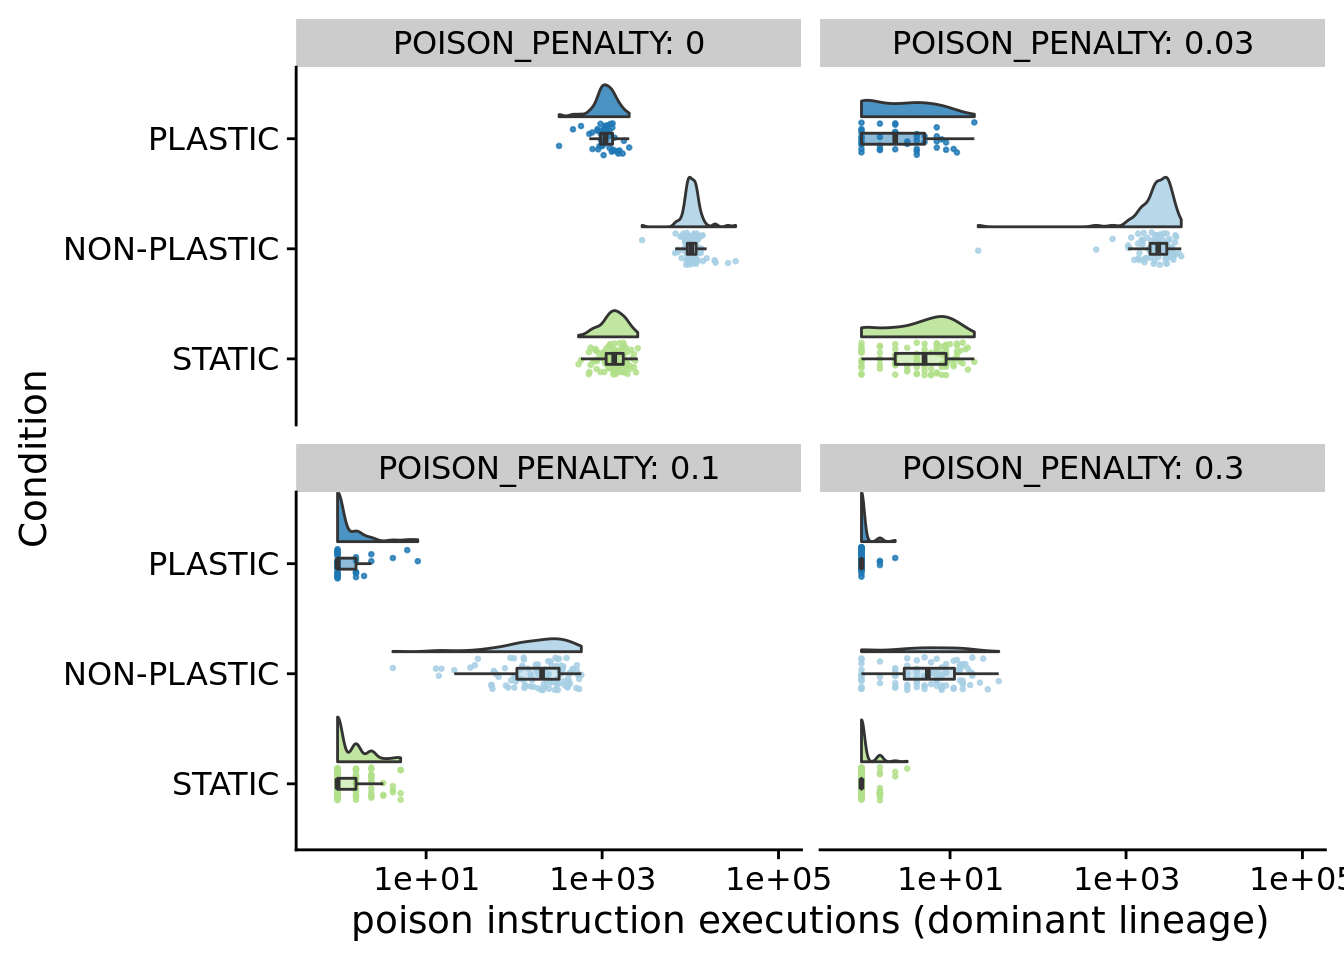
\includegraphics{supplemental-material_files/figure-latex/unnamed-chunk-89-1.pdf}

We can confirm our expectation that the dominant genotypes in non-plastic conditions are not phenotypically plastic.

\begin{Shaded}
\begin{Highlighting}[]
\NormalTok{summary_data_grouped =}\StringTok{ }\NormalTok{dplyr}\OperatorTok{::}\KeywordTok{group_by}\NormalTok{(summary_data, condition, is_plastic, POISON_PENALTY)}
\NormalTok{summary_data_group_counts =}\StringTok{ }\NormalTok{dplyr}\OperatorTok{::}\KeywordTok{summarize}\NormalTok{(summary_data_grouped, }\DataTypeTok{n=}\NormalTok{dplyr}\OperatorTok{::}\KeywordTok{n}\NormalTok{())}
\end{Highlighting}
\end{Shaded}

\begin{verbatim}
## `summarise()` has grouped output by 'condition', 'is_plastic'. You can override using the `.groups` argument.
\end{verbatim}

\begin{Shaded}
\begin{Highlighting}[]
\KeywordTok{ggplot}\NormalTok{(}\KeywordTok{filter}\NormalTok{(summary_data_group_counts, is_plastic), }\KeywordTok{aes}\NormalTok{(}\DataTypeTok{x=}\NormalTok{condition, }\DataTypeTok{y=}\NormalTok{n, }\DataTypeTok{fill=}\NormalTok{condition)) }\OperatorTok{+}
\StringTok{  }\KeywordTok{geom_col}\NormalTok{(}\DataTypeTok{position=}\KeywordTok{position_dodge}\NormalTok{(}\FloatTok{0.9}\NormalTok{)) }\OperatorTok{+}
\StringTok{  }\KeywordTok{scale_x_discrete}\NormalTok{(}
    \DataTypeTok{name=}\StringTok{"Condition"}\NormalTok{,}
    \DataTypeTok{limits=}\NormalTok{condition_order}
\NormalTok{  ) }\OperatorTok{+}
\StringTok{  }\KeywordTok{geom_text}\NormalTok{(}\KeywordTok{aes}\NormalTok{(}\DataTypeTok{label=}\NormalTok{n, }\DataTypeTok{y=}\NormalTok{n}\OperatorTok{+}\DecValTok{1}\NormalTok{)) }\OperatorTok{+}
\StringTok{  }\KeywordTok{ylab}\NormalTok{(}\StringTok{"Number of replicates with a plastic dominant genotype"}\NormalTok{) }\OperatorTok{+}
\StringTok{  }\KeywordTok{ylim}\NormalTok{(}\DecValTok{0}\NormalTok{, }\DecValTok{100}\NormalTok{) }\OperatorTok{+}
\StringTok{  }\KeywordTok{facet_wrap}\NormalTok{(}\OperatorTok{~}\NormalTok{POISON_PENALTY, }\DataTypeTok{labeller=}\NormalTok{label_both) }\OperatorTok{+}
\StringTok{  }\KeywordTok{theme}\NormalTok{(}
    \DataTypeTok{legend.position=}\StringTok{"none"}
\NormalTok{  )}
\end{Highlighting}
\end{Shaded}

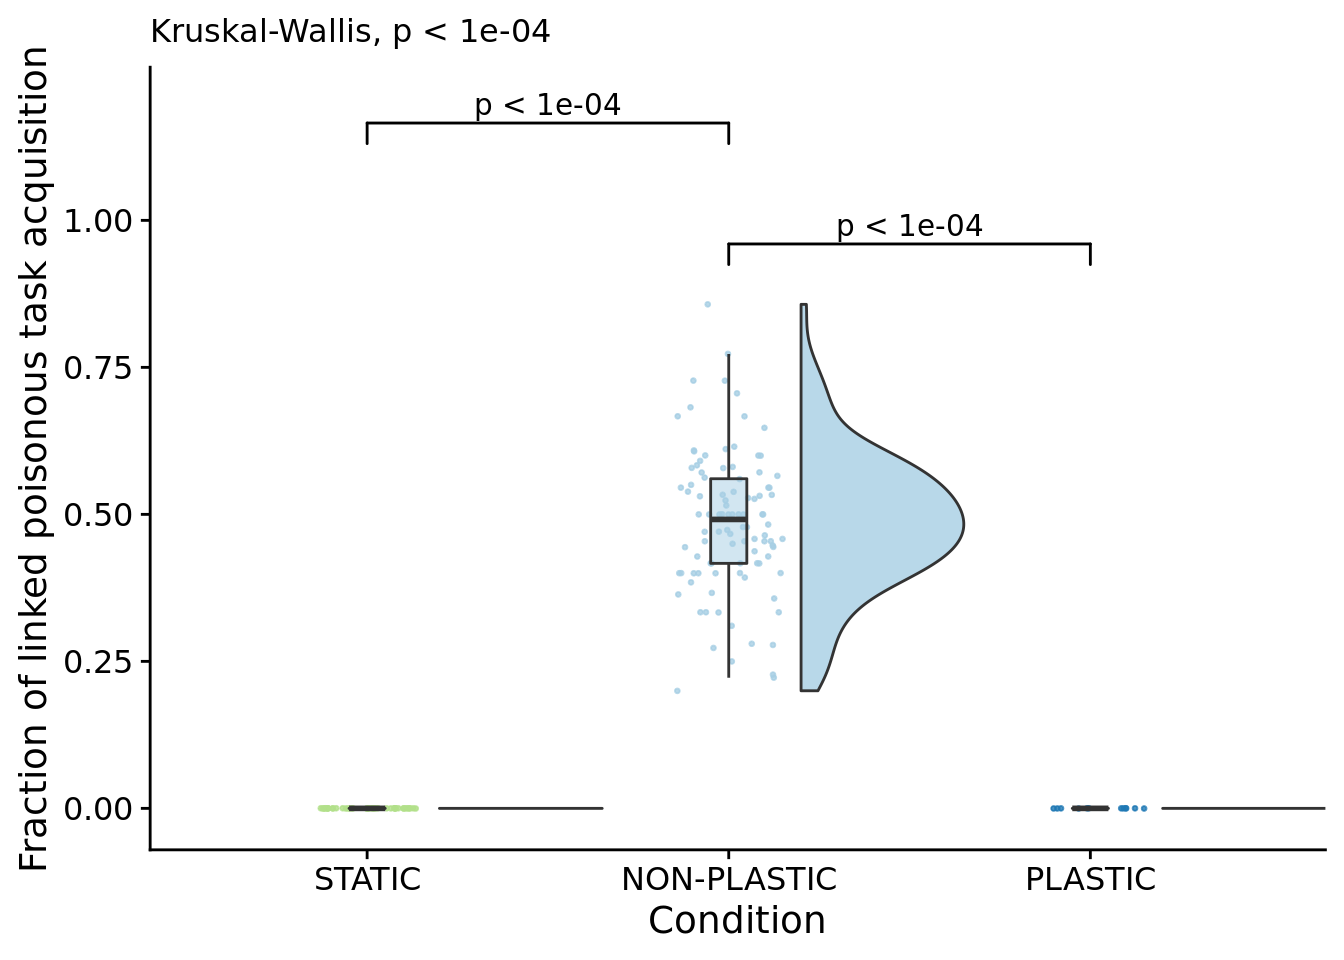
\includegraphics{supplemental-material_files/figure-latex/unnamed-chunk-90-1.pdf}

\hypertarget{hitchhiking-instruction-execution}{%
\section{Hitchhiking instruction execution}\label{hitchhiking-instruction-execution}}

\hypertarget{number-of-replicates-where-final-dominant-genotype-executes-hitchhiker-instruction}{%
\subsection{Number of replicates where final dominant genotype executes hitchhiker instruction}\label{number-of-replicates-where-final-dominant-genotype-executes-hitchhiker-instruction}}

\begin{Shaded}
\begin{Highlighting}[]
\NormalTok{hitchiker_penalty <-}\StringTok{ }\FloatTok{0.1}
\end{Highlighting}
\end{Shaded}

\begin{Shaded}
\begin{Highlighting}[]
\NormalTok{occurrences <-}\StringTok{ }\KeywordTok{c}\NormalTok{(}
  \KeywordTok{length}\NormalTok{(}\KeywordTok{filter}\NormalTok{(summary_data, POISON_PENALTY}\OperatorTok{==}\NormalTok{hitchiker_penalty }\OperatorTok{&}\StringTok{ }\NormalTok{condition}\OperatorTok{==}\StringTok{"NON-PLASTIC"} \OperatorTok{&}\StringTok{ }\NormalTok{dominant_times_poison_executed }\OperatorTok{>}\StringTok{ }\DecValTok{0}\NormalTok{)}\OperatorTok{$}\NormalTok{RANDOM_SEED),}
  \KeywordTok{length}\NormalTok{(}\KeywordTok{filter}\NormalTok{(summary_data, POISON_PENALTY}\OperatorTok{==}\NormalTok{hitchiker_penalty }\OperatorTok{&}\StringTok{ }\NormalTok{condition}\OperatorTok{==}\StringTok{"PLASTIC"} \OperatorTok{&}\StringTok{ }\NormalTok{dominant_times_poison_executed }\OperatorTok{>}\StringTok{ }\DecValTok{0}\NormalTok{)}\OperatorTok{$}\NormalTok{RANDOM_SEED),}
  \KeywordTok{length}\NormalTok{(}\KeywordTok{filter}\NormalTok{(summary_data, POISON_PENALTY}\OperatorTok{==}\NormalTok{hitchiker_penalty }\OperatorTok{&}\StringTok{ }\NormalTok{condition}\OperatorTok{==}\StringTok{"STATIC"} \OperatorTok{&}\StringTok{ }\NormalTok{dominant_times_poison_executed }\OperatorTok{>}\StringTok{ }\DecValTok{0}\NormalTok{)}\OperatorTok{$}\NormalTok{RANDOM_SEED)}
\NormalTok{)}
\NormalTok{trials <-}\StringTok{ }\KeywordTok{c}\NormalTok{(}
  \KeywordTok{length}\NormalTok{(}\KeywordTok{filter}\NormalTok{(summary_data, POISON_PENALTY}\OperatorTok{==}\NormalTok{hitchiker_penalty }\OperatorTok{&}\StringTok{ }\NormalTok{condition}\OperatorTok{==}\StringTok{"NON-PLASTIC"}\NormalTok{)}\OperatorTok{$}\NormalTok{RANDOM_SEED),}
  \KeywordTok{length}\NormalTok{(}\KeywordTok{filter}\NormalTok{(summary_data, POISON_PENALTY}\OperatorTok{==}\NormalTok{hitchiker_penalty }\OperatorTok{&}\StringTok{ }\NormalTok{condition}\OperatorTok{==}\StringTok{"PLASTIC"}\NormalTok{)}\OperatorTok{$}\NormalTok{RANDOM_SEED),}
  \KeywordTok{length}\NormalTok{(}\KeywordTok{filter}\NormalTok{(summary_data, POISON_PENALTY}\OperatorTok{==}\NormalTok{hitchiker_penalty }\OperatorTok{&}\StringTok{ }\NormalTok{condition}\OperatorTok{==}\StringTok{"STATIC"}\NormalTok{ )}\OperatorTok{$}\NormalTok{RANDOM_SEED)}
\NormalTok{)}
\KeywordTok{names}\NormalTok{(trials) <-}\StringTok{ }\KeywordTok{c}\NormalTok{(}
  \StringTok{"NON-PLASTIC"}\NormalTok{,}
  \StringTok{"PLASTIC"}\NormalTok{,}
  \StringTok{"STATIC"}
\NormalTok{)}
\KeywordTok{names}\NormalTok{(occurrences) <-}\StringTok{ }\KeywordTok{c}\NormalTok{(}
  \StringTok{"NON-PLASTIC"}\NormalTok{,}
  \StringTok{"PLASTIC"}\NormalTok{,}
  \StringTok{"STATIC"}
\NormalTok{)}

\KeywordTok{pairwise.fisher.test}\NormalTok{(}\DataTypeTok{x=}\NormalTok{occurrences, }\DataTypeTok{n=}\NormalTok{trials, }\DataTypeTok{p.adjust.method=}\StringTok{"bonferroni"}\NormalTok{)}
\end{Highlighting}
\end{Shaded}

\begin{verbatim}
## 
##  Pairwise comparisons using Pairwise comparison of proportions (Fisher) 
## 
## data:  occurrences out of trials 
## 
##         NON-PLASTIC PLASTIC
## PLASTIC 0.03212     -      
## STATIC  0.00022     1.00000
## 
## P value adjustment method: bonferroni
\end{verbatim}

\hypertarget{final-dominant-genotype-hitchhiker-execution}{%
\subsection{Final dominant genotype hitchhiker execution}\label{final-dominant-genotype-hitchhiker-execution}}

\begin{Shaded}
\begin{Highlighting}[]
\KeywordTok{ggplot}\NormalTok{(summary_data, }\KeywordTok{aes}\NormalTok{(}\DataTypeTok{x=}\NormalTok{condition, }\DataTypeTok{y=}\NormalTok{dominant_times_poison_executed, }\DataTypeTok{fill=}\NormalTok{condition)) }\OperatorTok{+}
\StringTok{  }\KeywordTok{geom_flat_violin}\NormalTok{(}
    \DataTypeTok{position =} \KeywordTok{position_nudge}\NormalTok{(}\DataTypeTok{x =} \FloatTok{.2}\NormalTok{, }\DataTypeTok{y =} \DecValTok{0}\NormalTok{),}
    \DataTypeTok{alpha =} \FloatTok{.8}
\NormalTok{  ) }\OperatorTok{+}
\StringTok{  }\KeywordTok{geom_point}\NormalTok{(}
    \DataTypeTok{mapping=}\KeywordTok{aes}\NormalTok{(}\DataTypeTok{color=}\NormalTok{condition),}
    \DataTypeTok{position =} \KeywordTok{position_jitter}\NormalTok{(}\DataTypeTok{width =} \FloatTok{.15}\NormalTok{),}
    \DataTypeTok{size =} \FloatTok{.5}\NormalTok{,}
    \DataTypeTok{alpha =} \FloatTok{0.8}
\NormalTok{  ) }\OperatorTok{+}
\StringTok{  }\KeywordTok{geom_boxplot}\NormalTok{(}
    \DataTypeTok{width =} \FloatTok{.1}\NormalTok{,}
    \DataTypeTok{outlier.shape =} \OtherTok{NA}\NormalTok{,}
    \DataTypeTok{alpha =} \FloatTok{0.5}
\NormalTok{  ) }\OperatorTok{+}
\StringTok{  }\KeywordTok{scale_x_discrete}\NormalTok{(}
    \DataTypeTok{name=}\StringTok{"Condition"}\NormalTok{,}
    \DataTypeTok{limits=}\NormalTok{condition_order}
\NormalTok{  ) }\OperatorTok{+}
\StringTok{  }\KeywordTok{ylab}\NormalTok{(}\StringTok{"poison instruction executions (final dominant)"}\NormalTok{) }\OperatorTok{+}
\StringTok{  }\KeywordTok{facet_wrap}\NormalTok{(}
    \OperatorTok{~}\NormalTok{POISON_PENALTY,}
    \DataTypeTok{labeller=}\NormalTok{label_both,}
    \DataTypeTok{scale=}\StringTok{"free_y"}
\NormalTok{  ) }\OperatorTok{+}
\StringTok{  }\KeywordTok{theme}\NormalTok{(}
    \DataTypeTok{legend.position=}\StringTok{"none"}
\NormalTok{  ) }\OperatorTok{+}
\StringTok{  }\KeywordTok{ggsave}\NormalTok{(}
    \KeywordTok{paste0}\NormalTok{(working_directory, }\StringTok{"plots/dominant-poison.pdf"}\NormalTok{),}
    \DataTypeTok{width=}\DecValTok{15}\NormalTok{,}
    \DataTypeTok{height=}\DecValTok{10}
\NormalTok{  )}
\end{Highlighting}
\end{Shaded}

\includegraphics{supplemental-material_files/figure-latex/unnamed-chunk-93-1.pdf}

\begin{Shaded}
\begin{Highlighting}[]
\NormalTok{penalties <-}\StringTok{ }\KeywordTok{levels}\NormalTok{(summary_data}\OperatorTok{$}\NormalTok{POISON_PENALTY)}
\ControlFlowTok{for}\NormalTok{ (penalty }\ControlFlowTok{in}\NormalTok{ penalties) \{}
\NormalTok{  stat_data <-}\StringTok{ }\KeywordTok{filter}\NormalTok{(summary_data, POISON_PENALTY}\OperatorTok{==}\NormalTok{penalty)}
  \KeywordTok{print}\NormalTok{(}
    \KeywordTok{paste0}\NormalTok{(}
      \StringTok{"PENALTY: "}\NormalTok{, penalty}
\NormalTok{    )}
\NormalTok{  )}
\NormalTok{  kt <-}\StringTok{ }\KeywordTok{kruskal.test}\NormalTok{(}
      \DataTypeTok{formula=}\NormalTok{dominant_times_poison_executed}\OperatorTok{~}\NormalTok{condition,}
      \DataTypeTok{data=}\NormalTok{stat_data}
\NormalTok{    )}
  \KeywordTok{print}\NormalTok{(}
\NormalTok{    kt}
\NormalTok{  )}
  \ControlFlowTok{if}\NormalTok{ (}\KeywordTok{is.na}\NormalTok{(kt}\OperatorTok{$}\NormalTok{p.value)) \{ }\ControlFlowTok{next}\NormalTok{ \}}
  \ControlFlowTok{if}\NormalTok{ (kt}\OperatorTok{$}\NormalTok{p.value }\OperatorTok{>}\StringTok{ }\FloatTok{0.05}\NormalTok{) \{ }\ControlFlowTok{next}\NormalTok{ \}}
  \KeywordTok{print}\NormalTok{(}
    \KeywordTok{pairwise.wilcox.test}\NormalTok{(}
      \DataTypeTok{x=}\NormalTok{stat_data}\OperatorTok{$}\NormalTok{dominant_times_poison_executed,}
      \DataTypeTok{g=}\NormalTok{stat_data}\OperatorTok{$}\NormalTok{condition,}
      \DataTypeTok{p.adjust.method=}\StringTok{"bonferroni"}
\NormalTok{    )}
\NormalTok{  )}
\NormalTok{\}}
\end{Highlighting}
\end{Shaded}

\begin{verbatim}
## [1] "PENALTY: 0"
## 
##  Kruskal-Wallis rank sum test
## 
## data:  dominant_times_poison_executed by condition
## Kruskal-Wallis chi-squared = 36.988, df = 2, p-value = 9.294e-09
## 
## 
##  Pairwise comparisons using Wilcoxon rank sum test with continuity correction 
## 
## data:  stat_data$dominant_times_poison_executed and stat_data$condition 
## 
##         NON-PLASTIC PLASTIC
## PLASTIC 2.8e-07     -      
## STATIC  0.00015     0.00198
## 
## P value adjustment method: bonferroni 
## [1] "PENALTY: 0.03"
## 
##  Kruskal-Wallis rank sum test
## 
## data:  dominant_times_poison_executed by condition
## Kruskal-Wallis chi-squared = 72.995, df = 2, p-value < 2.2e-16
## 
## 
##  Pairwise comparisons using Wilcoxon rank sum test with continuity correction 
## 
## data:  stat_data$dominant_times_poison_executed and stat_data$condition 
## 
##         NON-PLASTIC PLASTIC
## PLASTIC 2.0e-06     -      
## STATIC  2.8e-13     1      
## 
## P value adjustment method: bonferroni 
## [1] "PENALTY: 0.1"
## 
##  Kruskal-Wallis rank sum test
## 
## data:  dominant_times_poison_executed by condition
## Kruskal-Wallis chi-squared = 21.157, df = 2, p-value = 2.546e-05
## 
## 
##  Pairwise comparisons using Wilcoxon rank sum test with continuity correction 
## 
## data:  stat_data$dominant_times_poison_executed and stat_data$condition 
## 
##         NON-PLASTIC PLASTIC
## PLASTIC 0.02034     -      
## STATIC  0.00022     -      
## 
## P value adjustment method: bonferroni 
## [1] "PENALTY: 0.3"
## 
##  Kruskal-Wallis rank sum test
## 
## data:  dominant_times_poison_executed by condition
## Kruskal-Wallis chi-squared = NaN, df = 2, p-value = NA
\end{verbatim}

\hypertarget{hitchhiker-instruction-execution-in-final-population}{%
\subsection{Hitchhiker instruction execution in final population}\label{hitchhiker-instruction-execution-in-final-population}}

\begin{Shaded}
\begin{Highlighting}[]
\KeywordTok{ggplot}\NormalTok{(summary_data, }\KeywordTok{aes}\NormalTok{(}\DataTypeTok{x=}\NormalTok{condition, }\DataTypeTok{y=}\NormalTok{final_population_poison, }\DataTypeTok{fill=}\NormalTok{condition)) }\OperatorTok{+}
\StringTok{  }\KeywordTok{geom_flat_violin}\NormalTok{(}
    \DataTypeTok{position =} \KeywordTok{position_nudge}\NormalTok{(}\DataTypeTok{x =} \FloatTok{.2}\NormalTok{, }\DataTypeTok{y =} \DecValTok{0}\NormalTok{),}
    \DataTypeTok{alpha =} \FloatTok{.8}
\NormalTok{  ) }\OperatorTok{+}
\StringTok{  }\KeywordTok{geom_point}\NormalTok{(}
    \DataTypeTok{mapping=}\KeywordTok{aes}\NormalTok{(}\DataTypeTok{color=}\NormalTok{condition),}
    \DataTypeTok{position =} \KeywordTok{position_jitter}\NormalTok{(}\DataTypeTok{width =} \FloatTok{.15}\NormalTok{),}
    \DataTypeTok{size =} \FloatTok{.5}\NormalTok{,}
    \DataTypeTok{alpha =} \FloatTok{0.8}
\NormalTok{  ) }\OperatorTok{+}
\StringTok{  }\KeywordTok{geom_boxplot}\NormalTok{(}
    \DataTypeTok{width =} \FloatTok{.1}\NormalTok{,}
    \DataTypeTok{outlier.shape =} \OtherTok{NA}\NormalTok{,}
    \DataTypeTok{alpha =} \FloatTok{0.5}
\NormalTok{  ) }\OperatorTok{+}
\StringTok{  }\KeywordTok{scale_x_discrete}\NormalTok{(}
    \DataTypeTok{name=}\StringTok{"Condition"}\NormalTok{,}
    \DataTypeTok{limits=}\NormalTok{condition_order}
\NormalTok{  ) }\OperatorTok{+}
\StringTok{  }\KeywordTok{scale_y_continuous}\NormalTok{(}
    \DataTypeTok{name=}\StringTok{"poison instruction executions (final population)"}\NormalTok{,}
    \DataTypeTok{trans=}\StringTok{"pseudo_log"}\NormalTok{,}
    \DataTypeTok{breaks=}\KeywordTok{c}\NormalTok{(}\DecValTok{0}\NormalTok{,}\DecValTok{10}\NormalTok{,}\DecValTok{100}\NormalTok{,}\DecValTok{1000}\NormalTok{, }\DecValTok{10000}\NormalTok{, }\DecValTok{100000}\NormalTok{, }\DecValTok{1000000}\NormalTok{),}
    \DataTypeTok{limits=}\KeywordTok{c}\NormalTok{(}\OperatorTok{-}\DecValTok{1}\NormalTok{,}\DecValTok{1000000}\NormalTok{)}
\NormalTok{  ) }\OperatorTok{+}
\StringTok{  }\KeywordTok{facet_wrap}\NormalTok{(}
    \OperatorTok{~}\NormalTok{POISON_PENALTY,}
    \DataTypeTok{labeller=}\NormalTok{label_both}
\NormalTok{  ) }\OperatorTok{+}
\StringTok{  }\KeywordTok{theme}\NormalTok{(}
    \DataTypeTok{legend.position=}\StringTok{"none"}
\NormalTok{  ) }\OperatorTok{+}
\StringTok{  }\KeywordTok{ggsave}\NormalTok{(}
    \KeywordTok{paste0}\NormalTok{(working_directory, }\StringTok{"plots/final-population-poison-log.pdf"}\NormalTok{),}
    \DataTypeTok{width=}\DecValTok{15}\NormalTok{,}
    \DataTypeTok{height=}\DecValTok{10}
\NormalTok{  )}
\end{Highlighting}
\end{Shaded}

\includegraphics{supplemental-material_files/figure-latex/unnamed-chunk-95-1.pdf}

\begin{Shaded}
\begin{Highlighting}[]
\NormalTok{penalties <-}\StringTok{ }\KeywordTok{levels}\NormalTok{(summary_data}\OperatorTok{$}\NormalTok{POISON_PENALTY)}
\ControlFlowTok{for}\NormalTok{ (penalty }\ControlFlowTok{in}\NormalTok{ penalties) \{}
\NormalTok{  stat_data <-}\StringTok{ }\KeywordTok{filter}\NormalTok{(summary_data, POISON_PENALTY}\OperatorTok{==}\NormalTok{penalty)}
  \KeywordTok{print}\NormalTok{(}
    \KeywordTok{paste0}\NormalTok{(}
      \StringTok{"PENALTY: "}\NormalTok{, penalty}
\NormalTok{    )}
\NormalTok{  )}
\NormalTok{  kt <-}\StringTok{ }\KeywordTok{kruskal.test}\NormalTok{(}
      \DataTypeTok{formula=}\NormalTok{final_population_poison}\OperatorTok{~}\NormalTok{condition,}
      \DataTypeTok{data=}\NormalTok{stat_data}
\NormalTok{    )}
  \KeywordTok{print}\NormalTok{(}
\NormalTok{    kt}
\NormalTok{  )}
  \ControlFlowTok{if}\NormalTok{ (}\KeywordTok{is.na}\NormalTok{(kt}\OperatorTok{$}\NormalTok{p.value)) \{ }\ControlFlowTok{next}\NormalTok{ \}}
  \ControlFlowTok{if}\NormalTok{ (kt}\OperatorTok{$}\NormalTok{p.value }\OperatorTok{>}\StringTok{ }\FloatTok{0.05}\NormalTok{) \{ }\ControlFlowTok{next}\NormalTok{ \}}
  \KeywordTok{print}\NormalTok{(}
    \KeywordTok{pairwise.wilcox.test}\NormalTok{(}
      \DataTypeTok{x=}\NormalTok{stat_data}\OperatorTok{$}\NormalTok{final_population_poison,}
      \DataTypeTok{g=}\NormalTok{stat_data}\OperatorTok{$}\NormalTok{condition,}
      \DataTypeTok{p.adjust.method=}\StringTok{"bonferroni"}
\NormalTok{    )}
\NormalTok{  )}
\NormalTok{\}}
\end{Highlighting}
\end{Shaded}

\begin{verbatim}
## [1] "PENALTY: 0"
## 
##  Kruskal-Wallis rank sum test
## 
## data:  final_population_poison by condition
## Kruskal-Wallis chi-squared = 43.589, df = 2, p-value = 3.426e-10
## 
## 
##  Pairwise comparisons using Wilcoxon rank sum test with continuity correction 
## 
## data:  stat_data$final_population_poison and stat_data$condition 
## 
##         NON-PLASTIC PLASTIC
## PLASTIC 8.7e-07     -      
## STATIC  9.8e-07     0.00074
## 
## P value adjustment method: bonferroni 
## [1] "PENALTY: 0.03"
## 
##  Kruskal-Wallis rank sum test
## 
## data:  final_population_poison by condition
## Kruskal-Wallis chi-squared = 20.74, df = 2, p-value = 3.136e-05
## 
## 
##  Pairwise comparisons using Wilcoxon rank sum test with continuity correction 
## 
## data:  stat_data$final_population_poison and stat_data$condition 
## 
##         NON-PLASTIC PLASTIC
## PLASTIC 0.003       -      
## STATIC  1e-04       1.000  
## 
## P value adjustment method: bonferroni 
## [1] "PENALTY: 0.1"
## 
##  Kruskal-Wallis rank sum test
## 
## data:  final_population_poison by condition
## Kruskal-Wallis chi-squared = 20.608, df = 2, p-value = 3.35e-05
## 
## 
##  Pairwise comparisons using Wilcoxon rank sum test with continuity correction 
## 
## data:  stat_data$final_population_poison and stat_data$condition 
## 
##         NON-PLASTIC PLASTIC
## PLASTIC 0.0093      -      
## STATIC  4.9e-05     1.0000 
## 
## P value adjustment method: bonferroni 
## [1] "PENALTY: 0.3"
## 
##  Kruskal-Wallis rank sum test
## 
## data:  final_population_poison by condition
## Kruskal-Wallis chi-squared = 3.3994, df = 2, p-value = 0.1827
\end{verbatim}

\hypertarget{hitchhiker-instruction-execution-along-final-dominant-lineage-cummulative}{%
\subsection{Hitchhiker instruction execution along final dominant lineage (cummulative)}\label{hitchhiker-instruction-execution-along-final-dominant-lineage-cummulative}}

\begin{Shaded}
\begin{Highlighting}[]
\KeywordTok{ggplot}\NormalTok{(summary_data, }\KeywordTok{aes}\NormalTok{(}\DataTypeTok{x=}\NormalTok{condition, }\DataTypeTok{y=}\NormalTok{dominant_lineage_times_poison_executed, }\DataTypeTok{fill=}\NormalTok{condition)) }\OperatorTok{+}
\StringTok{  }\KeywordTok{geom_flat_violin}\NormalTok{(}
    \DataTypeTok{position =} \KeywordTok{position_nudge}\NormalTok{(}\DataTypeTok{x =} \FloatTok{.2}\NormalTok{, }\DataTypeTok{y =} \DecValTok{0}\NormalTok{),}
    \DataTypeTok{alpha =} \FloatTok{.8}
\NormalTok{  ) }\OperatorTok{+}
\StringTok{  }\KeywordTok{geom_point}\NormalTok{(}
    \DataTypeTok{mapping=}\KeywordTok{aes}\NormalTok{(}\DataTypeTok{color=}\NormalTok{condition),}
    \DataTypeTok{position =} \KeywordTok{position_jitter}\NormalTok{(}\DataTypeTok{width =} \FloatTok{.15}\NormalTok{),}
    \DataTypeTok{size =} \FloatTok{.5}\NormalTok{,}
    \DataTypeTok{alpha =} \FloatTok{0.8}
\NormalTok{  ) }\OperatorTok{+}
\StringTok{  }\KeywordTok{geom_boxplot}\NormalTok{(}
    \DataTypeTok{width =} \FloatTok{.1}\NormalTok{,}
    \DataTypeTok{outlier.shape =} \OtherTok{NA}\NormalTok{,}
    \DataTypeTok{alpha =} \FloatTok{0.5}
\NormalTok{  ) }\OperatorTok{+}
\StringTok{  }\KeywordTok{scale_x_discrete}\NormalTok{(}
    \DataTypeTok{name=}\StringTok{"Condition"}\NormalTok{,}
    \DataTypeTok{limits=}\NormalTok{condition_order}
\NormalTok{  ) }\OperatorTok{+}
\StringTok{  }\KeywordTok{scale_y_continuous}\NormalTok{(}
    \DataTypeTok{name=}\StringTok{"poison instruction executions (dominant lineage)"}\NormalTok{,}
    \DataTypeTok{trans=}\StringTok{"pseudo_log"}\NormalTok{,}
    \DataTypeTok{breaks=}\KeywordTok{c}\NormalTok{(}\DecValTok{0}\NormalTok{,}\DecValTok{10}\NormalTok{,}\DecValTok{100}\NormalTok{,}\DecValTok{1000}\NormalTok{,}\DecValTok{10000}\NormalTok{,}\DecValTok{100000}\NormalTok{),}
    \DataTypeTok{limits=}\KeywordTok{c}\NormalTok{(}\OperatorTok{-}\DecValTok{1}\NormalTok{,}\DecValTok{100000}\NormalTok{)}
\NormalTok{  ) }\OperatorTok{+}
\StringTok{  }\KeywordTok{facet_wrap}\NormalTok{(}
    \OperatorTok{~}\NormalTok{POISON_PENALTY,}
    \DataTypeTok{labeller=}\NormalTok{label_both}
\NormalTok{  ) }\OperatorTok{+}
\StringTok{  }\KeywordTok{theme}\NormalTok{(}
    \DataTypeTok{legend.position=}\StringTok{"none"}
\NormalTok{  ) }\OperatorTok{+}
\StringTok{  }\KeywordTok{ggsave}\NormalTok{(}
    \KeywordTok{paste0}\NormalTok{(working_directory, }\StringTok{"plots/final-dominant-lineage-poison-log.pdf"}\NormalTok{),}
    \DataTypeTok{width=}\DecValTok{15}\NormalTok{,}
    \DataTypeTok{height=}\DecValTok{10}
\NormalTok{  )}
\end{Highlighting}
\end{Shaded}

\includegraphics{supplemental-material_files/figure-latex/unnamed-chunk-97-1.pdf}

\begin{Shaded}
\begin{Highlighting}[]
\NormalTok{penalties <-}\StringTok{ }\KeywordTok{levels}\NormalTok{(summary_data}\OperatorTok{$}\NormalTok{POISON_PENALTY)}
\ControlFlowTok{for}\NormalTok{ (penalty }\ControlFlowTok{in}\NormalTok{ penalties) \{}
\NormalTok{  stat_data <-}\StringTok{ }\KeywordTok{filter}\NormalTok{(summary_data, POISON_PENALTY}\OperatorTok{==}\NormalTok{penalty)}
  \KeywordTok{print}\NormalTok{(}
    \KeywordTok{paste0}\NormalTok{(}
      \StringTok{"PENALTY: "}\NormalTok{, penalty}
\NormalTok{    )}
\NormalTok{  )}
\NormalTok{  kt <-}\StringTok{ }\KeywordTok{kruskal.test}\NormalTok{(}
      \DataTypeTok{formula=}\NormalTok{dominant_lineage_times_poison_executed}\OperatorTok{~}\NormalTok{condition,}
      \DataTypeTok{data=}\NormalTok{stat_data}
\NormalTok{    )}
  \KeywordTok{print}\NormalTok{(}
\NormalTok{    kt}
\NormalTok{  )}
  \ControlFlowTok{if}\NormalTok{ (}\KeywordTok{is.na}\NormalTok{(kt}\OperatorTok{$}\NormalTok{p.value)) \{ }\ControlFlowTok{next}\NormalTok{ \}}
  \ControlFlowTok{if}\NormalTok{ (kt}\OperatorTok{$}\NormalTok{p.value }\OperatorTok{>}\StringTok{ }\FloatTok{0.05}\NormalTok{) \{ }\ControlFlowTok{next}\NormalTok{ \}}
  \KeywordTok{print}\NormalTok{(}
    \KeywordTok{pairwise.wilcox.test}\NormalTok{(}
      \DataTypeTok{x=}\NormalTok{stat_data}\OperatorTok{$}\NormalTok{dominant_lineage_times_poison_executed,}
      \DataTypeTok{g=}\NormalTok{stat_data}\OperatorTok{$}\NormalTok{condition,}
      \DataTypeTok{p.adjust.method=}\StringTok{"bonferroni"}
\NormalTok{    )}
\NormalTok{  )}
\NormalTok{\}}
\end{Highlighting}
\end{Shaded}

\begin{verbatim}
## [1] "PENALTY: 0"
## 
##  Kruskal-Wallis rank sum test
## 
## data:  dominant_lineage_times_poison_executed by condition
## Kruskal-Wallis chi-squared = 178.84, df = 2, p-value < 2.2e-16
## 
## 
##  Pairwise comparisons using Wilcoxon rank sum test with continuity correction 
## 
## data:  stat_data$dominant_lineage_times_poison_executed and stat_data$condition 
## 
##         NON-PLASTIC PLASTIC
## PLASTIC <2e-16      -      
## STATIC  <2e-16      0.0018 
## 
## P value adjustment method: bonferroni 
## [1] "PENALTY: 0.03"
## 
##  Kruskal-Wallis rank sum test
## 
## data:  dominant_lineage_times_poison_executed by condition
## Kruskal-Wallis chi-squared = 178.62, df = 2, p-value < 2.2e-16
## 
## 
##  Pairwise comparisons using Wilcoxon rank sum test with continuity correction 
## 
## data:  stat_data$dominant_lineage_times_poison_executed and stat_data$condition 
## 
##         NON-PLASTIC PLASTIC
## PLASTIC <2e-16      -      
## STATIC  <2e-16      0.011  
## 
## P value adjustment method: bonferroni 
## [1] "PENALTY: 0.1"
## 
##  Kruskal-Wallis rank sum test
## 
## data:  dominant_lineage_times_poison_executed by condition
## Kruskal-Wallis chi-squared = 184.83, df = 2, p-value < 2.2e-16
## 
## 
##  Pairwise comparisons using Wilcoxon rank sum test with continuity correction 
## 
## data:  stat_data$dominant_lineage_times_poison_executed and stat_data$condition 
## 
##         NON-PLASTIC PLASTIC
## PLASTIC <2e-16      -      
## STATIC  <2e-16      0.21   
## 
## P value adjustment method: bonferroni 
## [1] "PENALTY: 0.3"
## 
##  Kruskal-Wallis rank sum test
## 
## data:  dominant_lineage_times_poison_executed by condition
## Kruskal-Wallis chi-squared = 149.48, df = 2, p-value < 2.2e-16
## 
## 
##  Pairwise comparisons using Wilcoxon rank sum test with continuity correction 
## 
## data:  stat_data$dominant_lineage_times_poison_executed and stat_data$condition 
## 
##         NON-PLASTIC PLASTIC
## PLASTIC 4.4e-16     -      
## STATIC  < 2e-16     0.84   
## 
## P value adjustment method: bonferroni
\end{verbatim}

\hypertarget{characterizing-mutations-that-increase-hitchhiker-instruction-execution}{%
\section{Characterizing mutations that increase hitchhiker instruction execution}\label{characterizing-mutations-that-increase-hitchhiker-instruction-execution}}

\hypertarget{number-of-offspring-along-dominant-lineage-with-increase-in-hitchiker-instruction-execution}{%
\subsection{Number of offspring along dominant lineage with increase in hitchiker instruction execution}\label{number-of-offspring-along-dominant-lineage-with-increase-in-hitchiker-instruction-execution}}

\begin{Shaded}
\begin{Highlighting}[]
\KeywordTok{ggplot}\NormalTok{(summary_data, }\KeywordTok{aes}\NormalTok{(}\DataTypeTok{x=}\NormalTok{condition, }\DataTypeTok{y=}\NormalTok{dominant_lineage_num_times_hitchhike_inst_exec_increases, }\DataTypeTok{fill=}\NormalTok{condition)) }\OperatorTok{+}
\StringTok{  }\KeywordTok{geom_flat_violin}\NormalTok{(}
    \DataTypeTok{position =} \KeywordTok{position_nudge}\NormalTok{(}\DataTypeTok{x =} \FloatTok{.2}\NormalTok{, }\DataTypeTok{y =} \DecValTok{0}\NormalTok{),}
    \DataTypeTok{alpha =} \FloatTok{.8}
\NormalTok{  ) }\OperatorTok{+}
\StringTok{  }\KeywordTok{geom_point}\NormalTok{(}
    \DataTypeTok{mapping=}\KeywordTok{aes}\NormalTok{(}\DataTypeTok{color=}\NormalTok{condition),}
    \DataTypeTok{position =} \KeywordTok{position_jitter}\NormalTok{(}\DataTypeTok{width =} \FloatTok{.15}\NormalTok{),}
    \DataTypeTok{size =} \FloatTok{.5}\NormalTok{,}
    \DataTypeTok{alpha =} \FloatTok{0.8}
\NormalTok{  ) }\OperatorTok{+}
\StringTok{  }\KeywordTok{geom_boxplot}\NormalTok{(}
    \DataTypeTok{width =} \FloatTok{.1}\NormalTok{,}
    \DataTypeTok{outlier.shape =} \OtherTok{NA}\NormalTok{,}
    \DataTypeTok{alpha =} \FloatTok{0.5}
\NormalTok{  ) }\OperatorTok{+}
\StringTok{  }\KeywordTok{scale_x_discrete}\NormalTok{(}
    \DataTypeTok{name=}\StringTok{"Condition"}\NormalTok{,}
    \DataTypeTok{limits=}\NormalTok{condition_order}
\NormalTok{  ) }\OperatorTok{+}
\StringTok{  }\KeywordTok{facet_wrap}\NormalTok{(}
    \OperatorTok{~}\NormalTok{POISON_PENALTY,}
    \DataTypeTok{labeller=}\NormalTok{label_both,}
    \DataTypeTok{scales=}\StringTok{"free_y"}
\NormalTok{  ) }\OperatorTok{+}
\StringTok{  }\KeywordTok{theme}\NormalTok{(}
    \DataTypeTok{legend.position=}\StringTok{"none"}
\NormalTok{  ) }\OperatorTok{+}
\StringTok{  }\KeywordTok{ggsave}\NormalTok{(}
    \KeywordTok{paste0}\NormalTok{(working_directory, }\StringTok{"plots/final-dominant-lineage-poison-increase-num-mutants-log.pdf"}\NormalTok{),}
    \DataTypeTok{width=}\DecValTok{15}\NormalTok{,}
    \DataTypeTok{height=}\DecValTok{10}
\NormalTok{  )}
\end{Highlighting}
\end{Shaded}

\includegraphics{supplemental-material_files/figure-latex/unnamed-chunk-99-1.pdf}

\begin{Shaded}
\begin{Highlighting}[]
\NormalTok{penalties <-}\StringTok{ }\KeywordTok{levels}\NormalTok{(summary_data}\OperatorTok{$}\NormalTok{POISON_PENALTY)}
\ControlFlowTok{for}\NormalTok{ (penalty }\ControlFlowTok{in}\NormalTok{ penalties) \{}
\NormalTok{  stat_data <-}\StringTok{ }\KeywordTok{filter}\NormalTok{(summary_data, POISON_PENALTY}\OperatorTok{==}\NormalTok{penalty)}
  \KeywordTok{print}\NormalTok{(}
    \KeywordTok{paste0}\NormalTok{(}
      \StringTok{"PENALTY: "}\NormalTok{, penalty}
\NormalTok{    )}
\NormalTok{  )}
\NormalTok{  kt <-}\StringTok{ }\KeywordTok{kruskal.test}\NormalTok{(}
      \DataTypeTok{formula=}\NormalTok{dominant_lineage_num_times_hitchhike_inst_exec_increases}\OperatorTok{~}\NormalTok{condition,}
      \DataTypeTok{data=}\NormalTok{stat_data}
\NormalTok{    )}
  \KeywordTok{print}\NormalTok{(}
\NormalTok{    kt}
\NormalTok{  )}
  \ControlFlowTok{if}\NormalTok{ (}\KeywordTok{is.na}\NormalTok{(kt}\OperatorTok{$}\NormalTok{p.value)) \{ }\ControlFlowTok{next}\NormalTok{ \}}
  \ControlFlowTok{if}\NormalTok{ (kt}\OperatorTok{$}\NormalTok{p.value }\OperatorTok{>}\StringTok{ }\FloatTok{0.05}\NormalTok{) \{ }\ControlFlowTok{next}\NormalTok{ \}}
  \KeywordTok{print}\NormalTok{(}
    \KeywordTok{pairwise.wilcox.test}\NormalTok{(}
      \DataTypeTok{x=}\NormalTok{stat_data}\OperatorTok{$}\NormalTok{dominant_lineage_num_times_hitchhike_inst_exec_increases,}
      \DataTypeTok{g=}\NormalTok{stat_data}\OperatorTok{$}\NormalTok{condition,}
      \DataTypeTok{p.adjust.method=}\StringTok{"bonferroni"}
\NormalTok{    )}
\NormalTok{  )}
\NormalTok{\}}
\end{Highlighting}
\end{Shaded}

\begin{verbatim}
## [1] "PENALTY: 0"
## 
##  Kruskal-Wallis rank sum test
## 
## data:  dominant_lineage_num_times_hitchhike_inst_exec_increases by condition
## Kruskal-Wallis chi-squared = 179.79, df = 2, p-value < 2.2e-16
## 
## 
##  Pairwise comparisons using Wilcoxon rank sum test with continuity correction 
## 
## data:  stat_data$dominant_lineage_num_times_hitchhike_inst_exec_increases and stat_data$condition 
## 
##         NON-PLASTIC PLASTIC
## PLASTIC < 2e-16     -      
## STATIC  < 2e-16     0.00046
## 
## P value adjustment method: bonferroni 
## [1] "PENALTY: 0.03"
## 
##  Kruskal-Wallis rank sum test
## 
## data:  dominant_lineage_num_times_hitchhike_inst_exec_increases by condition
## Kruskal-Wallis chi-squared = 179.35, df = 2, p-value < 2.2e-16
## 
## 
##  Pairwise comparisons using Wilcoxon rank sum test with continuity correction 
## 
## data:  stat_data$dominant_lineage_num_times_hitchhike_inst_exec_increases and stat_data$condition 
## 
##         NON-PLASTIC PLASTIC
## PLASTIC <2e-16      -      
## STATIC  <2e-16      0.03   
## 
## P value adjustment method: bonferroni 
## [1] "PENALTY: 0.1"
## 
##  Kruskal-Wallis rank sum test
## 
## data:  dominant_lineage_num_times_hitchhike_inst_exec_increases by condition
## Kruskal-Wallis chi-squared = 185.34, df = 2, p-value < 2.2e-16
## 
## 
##  Pairwise comparisons using Wilcoxon rank sum test with continuity correction 
## 
## data:  stat_data$dominant_lineage_num_times_hitchhike_inst_exec_increases and stat_data$condition 
## 
##         NON-PLASTIC PLASTIC
## PLASTIC <2e-16      -      
## STATIC  <2e-16      0.27   
## 
## P value adjustment method: bonferroni 
## [1] "PENALTY: 0.3"
## 
##  Kruskal-Wallis rank sum test
## 
## data:  dominant_lineage_num_times_hitchhike_inst_exec_increases by condition
## Kruskal-Wallis chi-squared = 146.35, df = 2, p-value < 2.2e-16
## 
## 
##  Pairwise comparisons using Wilcoxon rank sum test with continuity correction 
## 
## data:  stat_data$dominant_lineage_num_times_hitchhike_inst_exec_increases and stat_data$condition 
## 
##         NON-PLASTIC PLASTIC
## PLASTIC 7.8e-16     -      
## STATIC  < 2e-16     0.86   
## 
## P value adjustment method: bonferroni
\end{verbatim}

\begin{Shaded}
\begin{Highlighting}[]
\KeywordTok{sum}\NormalTok{(}\KeywordTok{filter}\NormalTok{(summary_data, condition}\OperatorTok{==}\StringTok{"NON-PLASTIC"} \OperatorTok{&}\StringTok{ }\NormalTok{POISON_PENALTY}\OperatorTok{==}\FloatTok{0.1}\NormalTok{)}\OperatorTok{$}\NormalTok{dominant_lineage_num_times_hitchhike_inst_exec_increases)}
\end{Highlighting}
\end{Shaded}

\begin{verbatim}
## [1] 1916
\end{verbatim}

\begin{Shaded}
\begin{Highlighting}[]
\KeywordTok{sum}\NormalTok{(}\KeywordTok{filter}\NormalTok{(summary_data, condition}\OperatorTok{==}\StringTok{"PLASTIC"} \OperatorTok{&}\StringTok{ }\NormalTok{POISON_PENALTY}\OperatorTok{==}\FloatTok{0.1}\NormalTok{)}\OperatorTok{$}\NormalTok{dominant_lineage_num_times_hitchhike_inst_exec_increases)}
\end{Highlighting}
\end{Shaded}

\begin{verbatim}
## [1] 18
\end{verbatim}

\begin{Shaded}
\begin{Highlighting}[]
\KeywordTok{sum}\NormalTok{(}\KeywordTok{filter}\NormalTok{(summary_data, condition}\OperatorTok{==}\StringTok{"STATIC"} \OperatorTok{&}\StringTok{ }\NormalTok{POISON_PENALTY}\OperatorTok{==}\FloatTok{0.1}\NormalTok{)}\OperatorTok{$}\NormalTok{dominant_lineage_num_times_hitchhike_inst_exec_increases)}
\end{Highlighting}
\end{Shaded}

\begin{verbatim}
## [1] 58
\end{verbatim}

\begin{Shaded}
\begin{Highlighting}[]
\CommentTok{# sum(filter(summary_data, condition=="NON-PLASTIC" & POISON_PENALTY==0.1)$dominant_lineage_trait_volatility)}
\CommentTok{# sum(filter(summary_data, condition=="PLASTIC" & POISON_PENALTY==0.1)$dominant_lineage_trait_volatility)}
\CommentTok{# sum(filter(summary_data, condition=="STATIC" & POISON_PENALTY==0.1)$dominant_lineage_trait_volatility)}
\end{Highlighting}
\end{Shaded}

\hypertarget{normalized-by-generations}{%
\subsubsection{Normalized by generations}\label{normalized-by-generations}}

\begin{Shaded}
\begin{Highlighting}[]
\NormalTok{summary_data}\OperatorTok{$}\NormalTok{dominant_lineage_num_times_hitchhike_inst_exec_increases_per_generation <-}\StringTok{ }\NormalTok{summary_data}\OperatorTok{$}\NormalTok{dominant_lineage_num_times_hitchhike_inst_exec_increases }\OperatorTok{/}\StringTok{ }\NormalTok{summary_data}\OperatorTok{$}\NormalTok{dominant_generation_born}
\KeywordTok{ggplot}\NormalTok{(summary_data, }\KeywordTok{aes}\NormalTok{(}\DataTypeTok{x=}\NormalTok{condition, }\DataTypeTok{y=}\NormalTok{dominant_lineage_num_times_hitchhike_inst_exec_increases_per_generation, }\DataTypeTok{fill=}\NormalTok{condition)) }\OperatorTok{+}
\StringTok{  }\KeywordTok{geom_flat_violin}\NormalTok{(}
    \DataTypeTok{position =} \KeywordTok{position_nudge}\NormalTok{(}\DataTypeTok{x =} \FloatTok{.2}\NormalTok{, }\DataTypeTok{y =} \DecValTok{0}\NormalTok{),}
    \DataTypeTok{alpha =} \FloatTok{.8}
\NormalTok{  ) }\OperatorTok{+}
\StringTok{  }\KeywordTok{geom_point}\NormalTok{(}
    \DataTypeTok{mapping=}\KeywordTok{aes}\NormalTok{(}\DataTypeTok{color=}\NormalTok{condition),}
    \DataTypeTok{position =} \KeywordTok{position_jitter}\NormalTok{(}\DataTypeTok{width =} \FloatTok{.15}\NormalTok{),}
    \DataTypeTok{size =} \FloatTok{.5}\NormalTok{,}
    \DataTypeTok{alpha =} \FloatTok{0.8}
\NormalTok{  ) }\OperatorTok{+}
\StringTok{  }\KeywordTok{geom_boxplot}\NormalTok{(}
    \DataTypeTok{width =} \FloatTok{.1}\NormalTok{,}
    \DataTypeTok{outlier.shape =} \OtherTok{NA}\NormalTok{,}
    \DataTypeTok{alpha =} \FloatTok{0.5}
\NormalTok{  ) }\OperatorTok{+}
\StringTok{  }\KeywordTok{scale_x_discrete}\NormalTok{(}
    \DataTypeTok{name=}\StringTok{"Condition"}\NormalTok{,}
    \DataTypeTok{limits=}\NormalTok{condition_order}
\NormalTok{  ) }\OperatorTok{+}
\StringTok{  }\KeywordTok{facet_wrap}\NormalTok{(}
    \OperatorTok{~}\NormalTok{POISON_PENALTY,}
    \DataTypeTok{labeller=}\NormalTok{label_both,}
    \DataTypeTok{scales=}\StringTok{"free_y"}
\NormalTok{  ) }\OperatorTok{+}
\StringTok{  }\KeywordTok{theme}\NormalTok{(}
    \DataTypeTok{legend.position=}\StringTok{"none"}
\NormalTok{  )}
\end{Highlighting}
\end{Shaded}

\includegraphics{supplemental-material_files/figure-latex/unnamed-chunk-101-1.pdf}

\begin{Shaded}
\begin{Highlighting}[]
\NormalTok{penalties <-}\StringTok{ }\KeywordTok{levels}\NormalTok{(summary_data}\OperatorTok{$}\NormalTok{POISON_PENALTY)}
\ControlFlowTok{for}\NormalTok{ (penalty }\ControlFlowTok{in}\NormalTok{ penalties) \{}
\NormalTok{  stat_data <-}\StringTok{ }\KeywordTok{filter}\NormalTok{(summary_data, POISON_PENALTY}\OperatorTok{==}\NormalTok{penalty)}
  \KeywordTok{print}\NormalTok{(}
    \KeywordTok{paste0}\NormalTok{(}
      \StringTok{"PENALTY: "}\NormalTok{, penalty}
\NormalTok{    )}
\NormalTok{  )}
\NormalTok{  kt <-}\StringTok{ }\KeywordTok{kruskal.test}\NormalTok{(}
      \DataTypeTok{formula=}\NormalTok{dominant_lineage_num_times_hitchhike_inst_exec_increases_per_generation}\OperatorTok{~}\NormalTok{condition,}
      \DataTypeTok{data=}\NormalTok{stat_data}
\NormalTok{    )}
  \KeywordTok{print}\NormalTok{(}
\NormalTok{    kt}
\NormalTok{  )}
  \ControlFlowTok{if}\NormalTok{ (}\KeywordTok{is.na}\NormalTok{(kt}\OperatorTok{$}\NormalTok{p.value)) \{ }\ControlFlowTok{next}\NormalTok{ \}}
  \ControlFlowTok{if}\NormalTok{ (kt}\OperatorTok{$}\NormalTok{p.value }\OperatorTok{>}\StringTok{ }\FloatTok{0.05}\NormalTok{) \{ }\ControlFlowTok{next}\NormalTok{ \}}
  \KeywordTok{print}\NormalTok{(}
    \KeywordTok{pairwise.wilcox.test}\NormalTok{(}
      \DataTypeTok{x=}\NormalTok{stat_data}\OperatorTok{$}\NormalTok{dominant_lineage_num_times_hitchhike_inst_exec_increases_per_generation,}
      \DataTypeTok{g=}\NormalTok{stat_data}\OperatorTok{$}\NormalTok{condition,}
      \DataTypeTok{p.adjust.method=}\StringTok{"bonferroni"}
\NormalTok{    )}
\NormalTok{  )}
\NormalTok{\}}
\end{Highlighting}
\end{Shaded}

\begin{verbatim}
## [1] "PENALTY: 0"
## 
##  Kruskal-Wallis rank sum test
## 
## data:  dominant_lineage_num_times_hitchhike_inst_exec_increases_per_generation by condition
## Kruskal-Wallis chi-squared = 180.05, df = 2, p-value < 2.2e-16
## 
## 
##  Pairwise comparisons using Wilcoxon rank sum test with continuity correction 
## 
## data:  stat_data$dominant_lineage_num_times_hitchhike_inst_exec_increases_per_generation and stat_data$condition 
## 
##         NON-PLASTIC PLASTIC
## PLASTIC < 2e-16     -      
## STATIC  < 2e-16     7.8e-05
## 
## P value adjustment method: bonferroni 
## [1] "PENALTY: 0.03"
## 
##  Kruskal-Wallis rank sum test
## 
## data:  dominant_lineage_num_times_hitchhike_inst_exec_increases_per_generation by condition
## Kruskal-Wallis chi-squared = 176.25, df = 2, p-value < 2.2e-16
## 
## 
##  Pairwise comparisons using Wilcoxon rank sum test with continuity correction 
## 
## data:  stat_data$dominant_lineage_num_times_hitchhike_inst_exec_increases_per_generation and stat_data$condition 
## 
##         NON-PLASTIC PLASTIC
## PLASTIC <2e-16      -      
## STATIC  <2e-16      0.019  
## 
## P value adjustment method: bonferroni 
## [1] "PENALTY: 0.1"
## 
##  Kruskal-Wallis rank sum test
## 
## data:  dominant_lineage_num_times_hitchhike_inst_exec_increases_per_generation by condition
## Kruskal-Wallis chi-squared = 184.17, df = 2, p-value < 2.2e-16
## 
## 
##  Pairwise comparisons using Wilcoxon rank sum test with continuity correction 
## 
## data:  stat_data$dominant_lineage_num_times_hitchhike_inst_exec_increases_per_generation and stat_data$condition 
## 
##         NON-PLASTIC PLASTIC
## PLASTIC <2e-16      -      
## STATIC  <2e-16      0.2    
## 
## P value adjustment method: bonferroni 
## [1] "PENALTY: 0.3"
## 
##  Kruskal-Wallis rank sum test
## 
## data:  dominant_lineage_num_times_hitchhike_inst_exec_increases_per_generation by condition
## Kruskal-Wallis chi-squared = 140.99, df = 2, p-value < 2.2e-16
## 
## 
##  Pairwise comparisons using Wilcoxon rank sum test with continuity correction 
## 
## data:  stat_data$dominant_lineage_num_times_hitchhike_inst_exec_increases_per_generation and stat_data$condition 
## 
##         NON-PLASTIC PLASTIC
## PLASTIC 2.2e-15     -      
## STATIC  < 2e-16     0.79   
## 
## P value adjustment method: bonferroni
\end{verbatim}

\hypertarget{what-fraction-of-mutations-that-increase-hitchhiker-instruction-execution-co-occur-with-base-trait-changes}{%
\subsection{What fraction of mutations that increase hitchhiker instruction execution co-occur with base trait changes?}\label{what-fraction-of-mutations-that-increase-hitchhiker-instruction-execution-co-occur-with-base-trait-changes}}

\begin{Shaded}
\begin{Highlighting}[]
\CommentTok{# Fraction of unexpressed vs expressed increases in hitchhiker instructions}
\NormalTok{summary_data}\OperatorTok{$}\NormalTok{frac_hitchhiking_linked_trait_change <-}\StringTok{ }\NormalTok{summary_data}\OperatorTok{$}\NormalTok{dominant_lineage_num_times_hitchhike_inst_exec_increases_with_primary_trait_change }\OperatorTok{/}\StringTok{ }\NormalTok{summary_data}\OperatorTok{$}\NormalTok{dominant_lineage_num_times_hitchhike_inst_exec_increases}

\KeywordTok{ggplot}\NormalTok{(}\KeywordTok{filter}\NormalTok{(summary_data, dominant_lineage_num_times_hitchhike_inst_exec_increases}\OperatorTok{>}\DecValTok{0}\NormalTok{ ), }\KeywordTok{aes}\NormalTok{(}\DataTypeTok{x=}\NormalTok{frac_hitchhiking_linked_trait_change)) }\OperatorTok{+}
\StringTok{  }\KeywordTok{geom_density}\NormalTok{() }\OperatorTok{+}
\StringTok{  }\KeywordTok{facet_grid}\NormalTok{(}
\NormalTok{    condition}\OperatorTok{~}\NormalTok{POISON_PENALTY,}
    \DataTypeTok{labeller=}\NormalTok{label_both,}
    \DataTypeTok{scales=}\StringTok{"free_y"}
\NormalTok{  ) }\OperatorTok{+}
\StringTok{  }\KeywordTok{theme}\NormalTok{(}
    \DataTypeTok{legend.position=}\StringTok{"none"}
\NormalTok{  ) }\OperatorTok{+}
\StringTok{  }\KeywordTok{ggsave}\NormalTok{(}
    \KeywordTok{paste0}\NormalTok{(working_directory, }\StringTok{"plots/dominant-lineage-frac_hitchhiking_linked_trait_change.pdf"}\NormalTok{),}
    \DataTypeTok{width=}\DecValTok{15}\NormalTok{,}
    \DataTypeTok{height=}\DecValTok{10}
\NormalTok{  )}
\end{Highlighting}
\end{Shaded}

\includegraphics{supplemental-material_files/figure-latex/unnamed-chunk-103-1.pdf}

\begin{Shaded}
\begin{Highlighting}[]
\KeywordTok{ggplot}\NormalTok{(}\KeywordTok{filter}\NormalTok{(summary_data, dominant_lineage_num_times_hitchhike_inst_exec_increases}\OperatorTok{>}\DecValTok{0}\NormalTok{ ), }\KeywordTok{aes}\NormalTok{(}\DataTypeTok{x=}\NormalTok{condition, }\DataTypeTok{y=}\NormalTok{frac_hitchhiking_linked_trait_change, }\DataTypeTok{fill=}\NormalTok{condition)) }\OperatorTok{+}
\StringTok{  }\KeywordTok{geom_flat_violin}\NormalTok{(}
    \DataTypeTok{position =} \KeywordTok{position_nudge}\NormalTok{(}\DataTypeTok{x =} \FloatTok{.2}\NormalTok{, }\DataTypeTok{y =} \DecValTok{0}\NormalTok{),}
    \DataTypeTok{alpha =} \FloatTok{.8}
\NormalTok{  ) }\OperatorTok{+}
\StringTok{  }\KeywordTok{geom_point}\NormalTok{(}
    \DataTypeTok{mapping=}\KeywordTok{aes}\NormalTok{(}\DataTypeTok{color=}\NormalTok{condition),}
    \DataTypeTok{position =} \KeywordTok{position_jitter}\NormalTok{(}\DataTypeTok{width =} \FloatTok{.15}\NormalTok{),}
    \DataTypeTok{size =} \FloatTok{.5}\NormalTok{,}
    \DataTypeTok{alpha =} \FloatTok{0.8}
\NormalTok{  ) }\OperatorTok{+}
\StringTok{  }\KeywordTok{geom_boxplot}\NormalTok{(}
    \DataTypeTok{width =} \FloatTok{.1}\NormalTok{,}
    \DataTypeTok{outlier.shape =} \OtherTok{NA}\NormalTok{,}
    \DataTypeTok{alpha =} \FloatTok{0.5}
\NormalTok{  ) }\OperatorTok{+}
\StringTok{  }\KeywordTok{scale_x_discrete}\NormalTok{(}
    \DataTypeTok{name=}\StringTok{"Condition"}\NormalTok{,}
    \DataTypeTok{limits=}\NormalTok{condition_order}
\NormalTok{  ) }\OperatorTok{+}
\StringTok{  }\KeywordTok{facet_wrap}\NormalTok{(}
    \OperatorTok{~}\NormalTok{POISON_PENALTY,}
    \DataTypeTok{labeller=}\NormalTok{label_both,}
    \DataTypeTok{scales=}\StringTok{"free_y"}
\NormalTok{  ) }\OperatorTok{+}
\StringTok{  }\KeywordTok{theme}\NormalTok{(}
    \DataTypeTok{legend.position=}\StringTok{"none"}
\NormalTok{  )}
\end{Highlighting}
\end{Shaded}

\includegraphics{supplemental-material_files/figure-latex/unnamed-chunk-103-2.pdf}

\begin{Shaded}
\begin{Highlighting}[]
\NormalTok{penalties <-}\StringTok{ }\KeywordTok{levels}\NormalTok{(summary_data}\OperatorTok{$}\NormalTok{POISON_PENALTY)}
\ControlFlowTok{for}\NormalTok{ (penalty }\ControlFlowTok{in}\NormalTok{ penalties) \{}
\NormalTok{  stat_data <-}\StringTok{ }\KeywordTok{filter}\NormalTok{(summary_data, POISON_PENALTY}\OperatorTok{==}\NormalTok{penalty }\OperatorTok{&}\StringTok{ }\NormalTok{dominant_lineage_num_times_hitchhike_inst_exec_increases}\OperatorTok{>}\DecValTok{0}\NormalTok{)}
  \KeywordTok{print}\NormalTok{(}
    \KeywordTok{paste0}\NormalTok{(}
      \StringTok{"PENALTY: "}\NormalTok{, penalty}
\NormalTok{    )}
\NormalTok{  )}
\NormalTok{  kt <-}\StringTok{ }\KeywordTok{kruskal.test}\NormalTok{(}
      \DataTypeTok{formula=}\NormalTok{frac_hitchhiking_linked_trait_change}\OperatorTok{~}\NormalTok{condition,}
      \DataTypeTok{data=}\NormalTok{stat_data}
\NormalTok{    )}
  \KeywordTok{print}\NormalTok{(}
\NormalTok{    kt}
\NormalTok{  )}
  \ControlFlowTok{if}\NormalTok{ (}\KeywordTok{is.na}\NormalTok{(kt}\OperatorTok{$}\NormalTok{p.value)) \{ }\ControlFlowTok{next}\NormalTok{ \}}
  \ControlFlowTok{if}\NormalTok{ (kt}\OperatorTok{$}\NormalTok{p.value }\OperatorTok{>}\StringTok{ }\FloatTok{0.05}\NormalTok{) \{ }\ControlFlowTok{next}\NormalTok{ \}}
  \KeywordTok{print}\NormalTok{(}
    \KeywordTok{pairwise.wilcox.test}\NormalTok{(}
      \DataTypeTok{x=}\NormalTok{stat_data}\OperatorTok{$}\NormalTok{frac_hitchhiking_linked_trait_change,}
      \DataTypeTok{g=}\NormalTok{stat_data}\OperatorTok{$}\NormalTok{condition,}
      \DataTypeTok{p.adjust.method=}\StringTok{"bonferroni"}\NormalTok{,}
      \DataTypeTok{exact=}\OtherTok{FALSE}
\NormalTok{    )}
\NormalTok{  )}
\NormalTok{\}}
\end{Highlighting}
\end{Shaded}

\begin{verbatim}
## [1] "PENALTY: 0"
## 
##  Kruskal-Wallis rank sum test
## 
## data:  frac_hitchhiking_linked_trait_change by condition
## Kruskal-Wallis chi-squared = 211.29, df = 2, p-value < 2.2e-16
## 
## 
##  Pairwise comparisons using Wilcoxon rank sum test with continuity correction 
## 
## data:  stat_data$frac_hitchhiking_linked_trait_change and stat_data$condition 
## 
##         NON-PLASTIC PLASTIC
## PLASTIC <2e-16      -      
## STATIC  <2e-16      0.031  
## 
## P value adjustment method: bonferroni 
## [1] "PENALTY: 0.03"
## 
##  Kruskal-Wallis rank sum test
## 
## data:  frac_hitchhiking_linked_trait_change by condition
## Kruskal-Wallis chi-squared = 186.88, df = 2, p-value < 2.2e-16
## 
## 
##  Pairwise comparisons using Wilcoxon rank sum test with continuity correction 
## 
## data:  stat_data$frac_hitchhiking_linked_trait_change and stat_data$condition 
## 
##         NON-PLASTIC PLASTIC
## PLASTIC 2.9e-16     -      
## STATIC  < 2e-16     -      
## 
## P value adjustment method: bonferroni 
## [1] "PENALTY: 0.1"
## 
##  Kruskal-Wallis rank sum test
## 
## data:  frac_hitchhiking_linked_trait_change by condition
## Kruskal-Wallis chi-squared = 113.72, df = 2, p-value < 2.2e-16
## 
## 
##  Pairwise comparisons using Wilcoxon rank sum test with continuity correction 
## 
## data:  stat_data$frac_hitchhiking_linked_trait_change and stat_data$condition 
## 
##         NON-PLASTIC PLASTIC
## PLASTIC 3.3e-08     -      
## STATIC  < 2e-16     -      
## 
## P value adjustment method: bonferroni 
## [1] "PENALTY: 0.3"
## 
##  Kruskal-Wallis rank sum test
## 
## data:  frac_hitchhiking_linked_trait_change by condition
## Kruskal-Wallis chi-squared = 34.791, df = 2, p-value = 2.788e-08
## 
## 
##  Pairwise comparisons using Wilcoxon rank sum test with continuity correction 
## 
## data:  stat_data$frac_hitchhiking_linked_trait_change and stat_data$condition 
## 
##         NON-PLASTIC PLASTIC
## PLASTIC 0.26        -      
## STATIC  2.4e-08     0.18   
## 
## P value adjustment method: bonferroni
\end{verbatim}

\begin{Shaded}
\begin{Highlighting}[]
\NormalTok{denom <-}\StringTok{ }\KeywordTok{sum}\NormalTok{(}\KeywordTok{filter}\NormalTok{(summary_data, condition}\OperatorTok{==}\StringTok{"NON-PLASTIC"} \OperatorTok{&}\StringTok{ }\NormalTok{POISON_PENALTY}\OperatorTok{==}\FloatTok{0.1}\NormalTok{)}\OperatorTok{$}\NormalTok{dominant_lineage_num_times_hitchhike_inst_exec_increases)}
\NormalTok{num <-}\StringTok{ }\KeywordTok{sum}\NormalTok{(}\KeywordTok{filter}\NormalTok{(summary_data, condition}\OperatorTok{==}\StringTok{"NON-PLASTIC"} \OperatorTok{&}\StringTok{ }\NormalTok{POISON_PENALTY}\OperatorTok{==}\FloatTok{0.1}\NormalTok{)}\OperatorTok{$}\NormalTok{dominant_lineage_num_times_hitchhike_inst_exec_increases_with_primary_trait_change)}
\KeywordTok{paste0}\NormalTok{(}\StringTok{"NON-PLASTIC: "}\NormalTok{, num}\OperatorTok{/}\NormalTok{denom, }\StringTok{"("}\NormalTok{, num, }\StringTok{"/"}\NormalTok{, denom, }\StringTok{")"}\NormalTok{)}
\end{Highlighting}
\end{Shaded}

\begin{verbatim}
## [1] "NON-PLASTIC: 0.498956158663883(956/1916)"
\end{verbatim}

\begin{Shaded}
\begin{Highlighting}[]
\NormalTok{denom <-}\StringTok{ }\KeywordTok{sum}\NormalTok{(}\KeywordTok{filter}\NormalTok{(summary_data, condition}\OperatorTok{==}\StringTok{"PLASTIC"} \OperatorTok{&}\StringTok{ }\NormalTok{POISON_PENALTY}\OperatorTok{==}\FloatTok{0.1}\NormalTok{)}\OperatorTok{$}\NormalTok{dominant_lineage_num_times_hitchhike_inst_exec_increases)}
\NormalTok{num <-}\StringTok{ }\KeywordTok{sum}\NormalTok{(}\KeywordTok{filter}\NormalTok{(summary_data, condition}\OperatorTok{==}\StringTok{"PLASTIC"} \OperatorTok{&}\StringTok{ }\NormalTok{POISON_PENALTY}\OperatorTok{==}\FloatTok{0.1}\NormalTok{)}\OperatorTok{$}\NormalTok{dominant_lineage_num_times_hitchhike_inst_exec_increases_with_primary_trait_change)}
\KeywordTok{paste0}\NormalTok{(}\StringTok{"PLASTIC: "}\NormalTok{, num}\OperatorTok{/}\NormalTok{denom, }\StringTok{" ("}\NormalTok{, num, }\StringTok{"/"}\NormalTok{, denom, }\StringTok{")"}\NormalTok{)}
\end{Highlighting}
\end{Shaded}

\begin{verbatim}
## [1] "PLASTIC: 0 (0/18)"
\end{verbatim}

\begin{Shaded}
\begin{Highlighting}[]
\NormalTok{denom <-}\StringTok{ }\KeywordTok{sum}\NormalTok{(}\KeywordTok{filter}\NormalTok{(summary_data, condition}\OperatorTok{==}\StringTok{"STATIC"} \OperatorTok{&}\StringTok{ }\NormalTok{POISON_PENALTY}\OperatorTok{==}\FloatTok{0.1}\NormalTok{)}\OperatorTok{$}\NormalTok{dominant_lineage_num_times_hitchhike_inst_exec_increases)}
\NormalTok{num <-}\StringTok{ }\KeywordTok{sum}\NormalTok{(}\KeywordTok{filter}\NormalTok{(summary_data, condition}\OperatorTok{==}\StringTok{"STATIC"} \OperatorTok{&}\StringTok{ }\NormalTok{POISON_PENALTY}\OperatorTok{==}\FloatTok{0.1}\NormalTok{)}\OperatorTok{$}\NormalTok{dominant_lineage_num_times_hitchhike_inst_exec_increases_with_primary_trait_change)}
\KeywordTok{paste0}\NormalTok{(}\StringTok{"STATIC: "}\NormalTok{, num}\OperatorTok{/}\NormalTok{denom, }\StringTok{" ("}\NormalTok{, num, }\StringTok{"/"}\NormalTok{, denom, }\StringTok{")"}\NormalTok{)}
\end{Highlighting}
\end{Shaded}

\begin{verbatim}
## [1] "STATIC: 0 (0/58)"
\end{verbatim}

\hypertarget{what-about-unexpressed-vs-expressed-trait-changes-in-plastic-populations}{%
\subsection{What about unexpressed vs expressed trait changes in plastic populations?}\label{what-about-unexpressed-vs-expressed-trait-changes-in-plastic-populations}}

\begin{Shaded}
\begin{Highlighting}[]
\NormalTok{summary_data}\OperatorTok{$}\NormalTok{frac_unexpressed_hitchhiker_inc <-}\StringTok{ }\NormalTok{summary_data}\OperatorTok{$}\NormalTok{dominant_lineage_num_times_hitchhike_inst_exec_increases_in_unexpressed_phenotype }\OperatorTok{/}\StringTok{ }\NormalTok{summary_data}\OperatorTok{$}\NormalTok{dominant_lineage_num_times_hitchhike_inst_exec_increases}
\NormalTok{summary_data}\OperatorTok{$}\NormalTok{frac_expressed_hitchiker_inc <-}\StringTok{ }\NormalTok{summary_data}\OperatorTok{$}\NormalTok{dominant_lineage_num_times_hitchhike_inst_exec_increases_in_expressed_phenotype }\OperatorTok{/}\StringTok{ }\NormalTok{summary_data}\OperatorTok{$}\NormalTok{dominant_lineage_num_times_hitchhike_inst_exec_increases}

\KeywordTok{ggplot}\NormalTok{(}\KeywordTok{filter}\NormalTok{(summary_data, dominant_lineage_num_times_hitchhike_inst_exec_increases}\OperatorTok{>}\DecValTok{0} \OperatorTok{&}\StringTok{ }\NormalTok{condition}\OperatorTok{==}\StringTok{"PLASTIC"}\NormalTok{), }\KeywordTok{aes}\NormalTok{(}\DataTypeTok{x=}\NormalTok{frac_unexpressed_hitchhiker_inc)) }\OperatorTok{+}
\StringTok{  }\KeywordTok{geom_density}\NormalTok{() }\OperatorTok{+}
\StringTok{  }\KeywordTok{facet_grid}\NormalTok{(}
\NormalTok{    condition}\OperatorTok{~}\NormalTok{POISON_PENALTY,}
    \DataTypeTok{labeller=}\NormalTok{label_both,}
    \DataTypeTok{scales=}\StringTok{"free_y"}
\NormalTok{  ) }\OperatorTok{+}
\StringTok{  }\KeywordTok{theme}\NormalTok{(}
    \DataTypeTok{legend.position=}\StringTok{"none"}
\NormalTok{  )}
\end{Highlighting}
\end{Shaded}

\includegraphics{supplemental-material_files/figure-latex/unnamed-chunk-105-1.pdf}

\begin{Shaded}
\begin{Highlighting}[]
\CommentTok{# ggplot(filter(summary_data, dominant_lineage_num_times_hitchhike_inst_exec_increases>0 & condition=="PLASTIC"), aes(x=frac_expressed_hitchiker_inc)) +}
\CommentTok{#   geom_density() +}
\CommentTok{#   facet_grid(}
\CommentTok{#     condition~POISON_PENALTY,}
\CommentTok{#     labeller=label_both,}
\CommentTok{#     scales="free_y"}
\CommentTok{#   ) +}
\CommentTok{#   theme(}
\CommentTok{#     legend.position="none"}
\CommentTok{#   )}
\end{Highlighting}
\end{Shaded}

\hypertarget{manuscript-figures-2}{%
\section{Manuscript figures}\label{manuscript-figures-2}}

\begin{Shaded}
\begin{Highlighting}[]
\NormalTok{hitchiker_penalty <-}\StringTok{ }\FloatTok{0.1}
\end{Highlighting}
\end{Shaded}

\begin{Shaded}
\begin{Highlighting}[]
\KeywordTok{ggplot}\NormalTok{(}\KeywordTok{filter}\NormalTok{(summary_data, POISON_PENALTY}\OperatorTok{==}\NormalTok{hitchiker_penalty }\OperatorTok{&}\StringTok{ }\NormalTok{condition}\OperatorTok{==}\StringTok{"NON-PLASTIC"} \OperatorTok{&}\StringTok{ }\NormalTok{dominant_times_poison_executed }\OperatorTok{>}\StringTok{ }\DecValTok{0}\NormalTok{), }\KeywordTok{aes}\NormalTok{(}\DataTypeTok{x=}\NormalTok{condition, }\DataTypeTok{fill=}\NormalTok{condition) ) }\OperatorTok{+}
\StringTok{  }\KeywordTok{geom_bar}\NormalTok{() }\OperatorTok{+}
\StringTok{  }\KeywordTok{geom_text}\NormalTok{(}
    \DataTypeTok{stat=}\StringTok{"count"}\NormalTok{,}
    \DataTypeTok{mapping=}\KeywordTok{aes}\NormalTok{(}\DataTypeTok{label=}\NormalTok{..count..),}
    \DataTypeTok{position=}\KeywordTok{position_dodge}\NormalTok{(}\FloatTok{0.9}\NormalTok{),}
    \DataTypeTok{vjust=}\DecValTok{0}
\NormalTok{  ) }\OperatorTok{+}
\StringTok{  }\KeywordTok{scale_y_continuous}\NormalTok{(}
    \DataTypeTok{name=}\StringTok{"Number of replicates where poison is executed by dominant genotype"}\NormalTok{,}
    \DataTypeTok{limits=}\KeywordTok{c}\NormalTok{(}\DecValTok{0}\NormalTok{, replicates}\OperatorTok{+}\DecValTok{2}\NormalTok{)}
\NormalTok{  ) }\OperatorTok{+}
\StringTok{  }\KeywordTok{scale_x_discrete}\NormalTok{(}
    \DataTypeTok{name=}\StringTok{"Condition"}\NormalTok{,}
    \DataTypeTok{limits=}\NormalTok{condition_order,}
    \DataTypeTok{labels=}\NormalTok{condition_order,}
    \DataTypeTok{breaks=}\NormalTok{condition_order}
\NormalTok{  ) }\OperatorTok{+}
\StringTok{  }\KeywordTok{scale_fill_brewer}\NormalTok{(}
    \DataTypeTok{palette=}\StringTok{"Paired"}
\NormalTok{  ) }\OperatorTok{+}
\StringTok{  }\KeywordTok{scale_color_brewer}\NormalTok{(}
    \DataTypeTok{palette=}\StringTok{"Paired"}
\NormalTok{  ) }\OperatorTok{+}
\StringTok{  }\KeywordTok{coord_flip}\NormalTok{() }\OperatorTok{+}
\StringTok{  }\KeywordTok{theme}\NormalTok{(}
    \DataTypeTok{legend.position=}\StringTok{"none"}
\NormalTok{  )}
\end{Highlighting}
\end{Shaded}

\includegraphics{supplemental-material_files/figure-latex/unnamed-chunk-107-1.pdf}

\begin{Shaded}
\begin{Highlighting}[]
\NormalTok{fig_data <-}\StringTok{ }\KeywordTok{data.frame}\NormalTok{(}
  \DataTypeTok{num_execute_poison=}\KeywordTok{c}\NormalTok{(}
    \KeywordTok{length}\NormalTok{(}\KeywordTok{filter}\NormalTok{(summary_data, POISON_PENALTY}\OperatorTok{==}\NormalTok{hitchiker_penalty }\OperatorTok{&}\StringTok{ }\NormalTok{condition}\OperatorTok{==}\StringTok{"NON-PLASTIC"} \OperatorTok{&}\StringTok{ }\NormalTok{dominant_times_poison_executed }\OperatorTok{>}\StringTok{ }\DecValTok{0}\NormalTok{)}\OperatorTok{$}\NormalTok{RANDOM_SEED),}
    \KeywordTok{length}\NormalTok{(}\KeywordTok{filter}\NormalTok{(summary_data, POISON_PENALTY}\OperatorTok{==}\NormalTok{hitchiker_penalty }\OperatorTok{&}\StringTok{ }\NormalTok{condition}\OperatorTok{==}\StringTok{"PLASTIC"} \OperatorTok{&}\StringTok{ }\NormalTok{dominant_times_poison_executed }\OperatorTok{>}\StringTok{ }\DecValTok{0}\NormalTok{)}\OperatorTok{$}\NormalTok{RANDOM_SEED),}
    \KeywordTok{length}\NormalTok{(}\KeywordTok{filter}\NormalTok{(summary_data, POISON_PENALTY}\OperatorTok{==}\NormalTok{hitchiker_penalty }\OperatorTok{&}\StringTok{ }\NormalTok{condition}\OperatorTok{==}\StringTok{"STATIC"} \OperatorTok{&}\StringTok{ }\NormalTok{dominant_times_poison_executed }\OperatorTok{>}\StringTok{ }\DecValTok{0}\NormalTok{)}\OperatorTok{$}\NormalTok{RANDOM_SEED)}
\NormalTok{  ),}
  \DataTypeTok{num_execute_no_poison=}\KeywordTok{c}\NormalTok{(}
    \KeywordTok{length}\NormalTok{(}\KeywordTok{filter}\NormalTok{(summary_data, POISON_PENALTY}\OperatorTok{==}\NormalTok{hitchiker_penalty }\OperatorTok{&}\StringTok{ }\NormalTok{condition}\OperatorTok{==}\StringTok{"NON-PLASTIC"} \OperatorTok{&}\StringTok{ }\NormalTok{dominant_times_poison_executed }\OperatorTok{==}\StringTok{ }\DecValTok{0}\NormalTok{)}\OperatorTok{$}\NormalTok{RANDOM_SEED),}
    \KeywordTok{length}\NormalTok{(}\KeywordTok{filter}\NormalTok{(summary_data, POISON_PENALTY}\OperatorTok{==}\NormalTok{hitchiker_penalty }\OperatorTok{&}\StringTok{ }\NormalTok{condition}\OperatorTok{==}\StringTok{"PLASTIC"} \OperatorTok{&}\StringTok{ }\NormalTok{dominant_times_poison_executed }\OperatorTok{==}\StringTok{ }\DecValTok{0}\NormalTok{)}\OperatorTok{$}\NormalTok{RANDOM_SEED),}
    \KeywordTok{length}\NormalTok{(}\KeywordTok{filter}\NormalTok{(summary_data, POISON_PENALTY}\OperatorTok{==}\NormalTok{hitchiker_penalty }\OperatorTok{&}\StringTok{ }\NormalTok{condition}\OperatorTok{==}\StringTok{"STATIC"} \OperatorTok{&}\StringTok{ }\NormalTok{dominant_times_poison_executed }\OperatorTok{==}\StringTok{ }\DecValTok{0}\NormalTok{)}\OperatorTok{$}\NormalTok{RANDOM_SEED)}
\NormalTok{  ),}
  \DataTypeTok{total=}\KeywordTok{c}\NormalTok{(}
    \KeywordTok{length}\NormalTok{(}\KeywordTok{filter}\NormalTok{(summary_data, POISON_PENALTY}\OperatorTok{==}\NormalTok{hitchiker_penalty }\OperatorTok{&}\StringTok{ }\NormalTok{condition}\OperatorTok{==}\StringTok{"NON-PLASTIC"}\NormalTok{)}\OperatorTok{$}\NormalTok{RANDOM_SEED),}
    \KeywordTok{length}\NormalTok{(}\KeywordTok{filter}\NormalTok{(summary_data, POISON_PENALTY}\OperatorTok{==}\NormalTok{hitchiker_penalty }\OperatorTok{&}\StringTok{ }\NormalTok{condition}\OperatorTok{==}\StringTok{"PLASTIC"}\NormalTok{)}\OperatorTok{$}\NormalTok{RANDOM_SEED),}
    \KeywordTok{length}\NormalTok{(}\KeywordTok{filter}\NormalTok{(summary_data, POISON_PENALTY}\OperatorTok{==}\NormalTok{hitchiker_penalty }\OperatorTok{&}\StringTok{ }\NormalTok{condition}\OperatorTok{==}\StringTok{"STATIC"}\NormalTok{ )}\OperatorTok{$}\NormalTok{RANDOM_SEED)}
\NormalTok{  ),}
  \DataTypeTok{condition=}\KeywordTok{c}\NormalTok{(}
    \StringTok{"NON-PLASTIC"}\NormalTok{,}
    \StringTok{"PLASTIC"}\NormalTok{,}
    \StringTok{"STATIC"}
\NormalTok{  )}
\NormalTok{)}

\KeywordTok{ggplot}\NormalTok{(fig_data, }\KeywordTok{aes}\NormalTok{(}\DataTypeTok{x=}\NormalTok{condition, }\DataTypeTok{y=}\NormalTok{num_execute_poison, }\DataTypeTok{fill=}\NormalTok{condition)) }\OperatorTok{+}
\StringTok{  }\KeywordTok{geom_col}\NormalTok{(}\DataTypeTok{position=}\KeywordTok{position_dodge}\NormalTok{(}\FloatTok{0.9}\NormalTok{)) }\OperatorTok{+}
\StringTok{  }\KeywordTok{geom_text}\NormalTok{(}\KeywordTok{aes}\NormalTok{(}\DataTypeTok{label=}\NormalTok{num_execute_poison, }\DataTypeTok{y=}\NormalTok{num_execute_poison}\FloatTok{+0.25}\NormalTok{)) }\OperatorTok{+}
\StringTok{  }\KeywordTok{scale_x_discrete}\NormalTok{(}
    \DataTypeTok{name=}\StringTok{"Condition"}\NormalTok{,}
    \DataTypeTok{limits=}\NormalTok{condition_order}
\NormalTok{  ) }\OperatorTok{+}
\StringTok{  }\KeywordTok{scale_fill_brewer}\NormalTok{(}
    \DataTypeTok{palette=}\StringTok{"Paired"}
\NormalTok{  ) }\OperatorTok{+}
\StringTok{  }\KeywordTok{scale_color_brewer}\NormalTok{(}
    \DataTypeTok{palette=}\StringTok{"Paired"}
\NormalTok{  ) }\OperatorTok{+}
\StringTok{  }\KeywordTok{theme}\NormalTok{(}
    \DataTypeTok{legend.position=}\StringTok{"none"}
\NormalTok{  )}
\end{Highlighting}
\end{Shaded}

\includegraphics{supplemental-material_files/figure-latex/unnamed-chunk-107-2.pdf}

Number of poison increases along lineage.

\begin{Shaded}
\begin{Highlighting}[]
\NormalTok{poison_increases_fig <-}\StringTok{ }\KeywordTok{ggplot}\NormalTok{(}
    \KeywordTok{filter}\NormalTok{(summary_data, POISON_PENALTY}\OperatorTok{==}\NormalTok{hitchiker_penalty),}
    \KeywordTok{aes}\NormalTok{(}\DataTypeTok{x=}\NormalTok{condition, }\DataTypeTok{y=}\NormalTok{dominant_lineage_num_times_hitchhike_inst_exec_increases, }\DataTypeTok{fill=}\NormalTok{condition)}
\NormalTok{  ) }\OperatorTok{+}
\StringTok{  }\KeywordTok{geom_flat_violin}\NormalTok{(}
    \DataTypeTok{position =} \KeywordTok{position_nudge}\NormalTok{(}\DataTypeTok{x =} \FloatTok{.2}\NormalTok{, }\DataTypeTok{y =} \DecValTok{0}\NormalTok{),}
    \DataTypeTok{alpha =} \FloatTok{.8}
\NormalTok{  ) }\OperatorTok{+}
\StringTok{  }\KeywordTok{geom_point}\NormalTok{(}
    \DataTypeTok{mapping=}\KeywordTok{aes}\NormalTok{(}\DataTypeTok{color=}\NormalTok{condition),}
    \DataTypeTok{position =} \KeywordTok{position_jitter}\NormalTok{(}\DataTypeTok{width =} \FloatTok{.15}\NormalTok{),}
    \DataTypeTok{size =} \FloatTok{.5}\NormalTok{,}
    \DataTypeTok{alpha =} \FloatTok{0.8}
\NormalTok{  ) }\OperatorTok{+}
\StringTok{  }\KeywordTok{geom_boxplot}\NormalTok{(}
    \DataTypeTok{width =} \FloatTok{.1}\NormalTok{,}
    \DataTypeTok{outlier.shape =} \OtherTok{NA}\NormalTok{,}
    \DataTypeTok{alpha =} \FloatTok{0.5}
\NormalTok{  ) }\OperatorTok{+}
\StringTok{  }\KeywordTok{scale_x_discrete}\NormalTok{(}
    \DataTypeTok{name=}\StringTok{"Condition"}\NormalTok{,}
    \DataTypeTok{limits=}\NormalTok{condition_order,}
    \DataTypeTok{labels=}\NormalTok{condition_order}
\NormalTok{  ) }\OperatorTok{+}
\StringTok{  }\KeywordTok{scale_y_continuous}\NormalTok{(}
    \DataTypeTok{name=}\StringTok{"Increases in poison instruction execution along lineage"}\NormalTok{,}
\NormalTok{  ) }\OperatorTok{+}
\StringTok{  }\KeywordTok{scale_fill_brewer}\NormalTok{(}
    \DataTypeTok{palette=}\StringTok{"Paired"}
\NormalTok{  ) }\OperatorTok{+}
\StringTok{  }\KeywordTok{scale_color_brewer}\NormalTok{(}
    \DataTypeTok{palette=}\StringTok{"Paired"}
\NormalTok{  ) }\OperatorTok{+}
\StringTok{  }\KeywordTok{theme}\NormalTok{(}
    \DataTypeTok{legend.position=}\StringTok{"none"}
\NormalTok{  ) }\OperatorTok{+}
\StringTok{  }\KeywordTok{coord_flip}\NormalTok{()}

\NormalTok{poison_increases_fig}
\end{Highlighting}
\end{Shaded}

\includegraphics{supplemental-material_files/figure-latex/unnamed-chunk-108-1.pdf}

\begin{Shaded}
\begin{Highlighting}[]
\NormalTok{poison_increases_per_gen_fig <-}\StringTok{ }\KeywordTok{ggplot}\NormalTok{(}
    \KeywordTok{filter}\NormalTok{(summary_data, POISON_PENALTY}\OperatorTok{==}\NormalTok{hitchiker_penalty),}
    \KeywordTok{aes}\NormalTok{(}\DataTypeTok{x=}\NormalTok{condition, }\DataTypeTok{y=}\NormalTok{dominant_lineage_num_times_hitchhike_inst_exec_increases_per_generation, }\DataTypeTok{fill=}\NormalTok{condition)}
\NormalTok{  ) }\OperatorTok{+}
\StringTok{  }\KeywordTok{geom_flat_violin}\NormalTok{(}
    \DataTypeTok{position =} \KeywordTok{position_nudge}\NormalTok{(}\DataTypeTok{x =} \FloatTok{.2}\NormalTok{, }\DataTypeTok{y =} \DecValTok{0}\NormalTok{),}
    \DataTypeTok{alpha =} \FloatTok{.8}
\NormalTok{  ) }\OperatorTok{+}
\StringTok{  }\KeywordTok{geom_point}\NormalTok{(}
    \DataTypeTok{mapping=}\KeywordTok{aes}\NormalTok{(}\DataTypeTok{color=}\NormalTok{condition),}
    \DataTypeTok{position =} \KeywordTok{position_jitter}\NormalTok{(}\DataTypeTok{width =} \FloatTok{.15}\NormalTok{),}
    \DataTypeTok{size =} \FloatTok{.5}\NormalTok{,}
    \DataTypeTok{alpha =} \FloatTok{0.8}
\NormalTok{  ) }\OperatorTok{+}
\StringTok{  }\KeywordTok{geom_boxplot}\NormalTok{(}
    \DataTypeTok{width =} \FloatTok{.1}\NormalTok{,}
    \DataTypeTok{outlier.shape =} \OtherTok{NA}\NormalTok{,}
    \DataTypeTok{alpha =} \FloatTok{0.5}
\NormalTok{  ) }\OperatorTok{+}
\StringTok{  }\KeywordTok{scale_x_discrete}\NormalTok{(}
    \DataTypeTok{name=}\StringTok{"Condition"}\NormalTok{,}
    \DataTypeTok{limits=}\NormalTok{condition_order,}
    \DataTypeTok{labels=}\NormalTok{condition_order}
\NormalTok{  ) }\OperatorTok{+}
\StringTok{  }\KeywordTok{scale_y_continuous}\NormalTok{(}
    \DataTypeTok{name=}\StringTok{"Increases in poison instruction execution along lineage (per generation)"}\NormalTok{,}
\NormalTok{  ) }\OperatorTok{+}
\StringTok{  }\KeywordTok{scale_fill_brewer}\NormalTok{(}
    \DataTypeTok{palette=}\StringTok{"Paired"}
\NormalTok{  ) }\OperatorTok{+}
\StringTok{  }\KeywordTok{scale_color_brewer}\NormalTok{(}
    \DataTypeTok{palette=}\StringTok{"Paired"}
\NormalTok{  ) }\OperatorTok{+}
\StringTok{  }\KeywordTok{theme}\NormalTok{(}
    \DataTypeTok{legend.position=}\StringTok{"none"}
\NormalTok{  ) }\OperatorTok{+}
\StringTok{  }\KeywordTok{coord_flip}\NormalTok{()}

\NormalTok{poison_increases_per_gen_fig}
\end{Highlighting}
\end{Shaded}

\includegraphics{supplemental-material_files/figure-latex/unnamed-chunk-109-1.pdf}

Pull it all together.

\begin{Shaded}
\begin{Highlighting}[]
\CommentTok{# grid <- plot_grid(}
\CommentTok{#   dominant_extra_tasks_fig,}
\CommentTok{#   lineage_extra_tasks_discovered_fig + theme(axis.ticks.y=element_blank(),axis.text.y=element_blank(),axis.title.y=element_blank()),}
\CommentTok{#   lineage_extra_tasks_lost_fig + theme(axis.ticks.y=element_blank(),axis.text.y=element_blank(),axis.title.y=element_blank()),}
\CommentTok{#   nrow=1,}
\CommentTok{#   align="v",}
\CommentTok{#   labels="auto"}
\CommentTok{# )}
\CommentTok{# save_plot(}
\CommentTok{#    paste0(working_directory, "plots/", "complex-traits-panel.pdf"),}
\CommentTok{#    grid,}
\CommentTok{#    base_height=6,}
\CommentTok{#    base_asp=2.5}
\CommentTok{# )}
\CommentTok{# grid}
\end{Highlighting}
\end{Shaded}

\bibliography{packages.bib,supplemental.bib}

\end{document}
